% !TeX document-id = {8ebe89f4-14fa-44c3-a184-4e485a4d4b1b}
% !TEX spellcheck = English (United States) (Aspell)
% !TEX TS-program = arara
%  arara: clean   : { extensions: [aux,bbl,bcf,blg,glg,glo,gls,idx,ilg,ind,ist,log,lof,lol,lot,out,ptc,toc,run.xml] }
%  arara: pdflatex: {               options: ['-file-line-error','-halt-on-error','-ini','"&pdflatex"','mylatexformat.ltx'] }
%  arara: pdflatex: {   draft: yes, options: ['-file-line-error','-halt-on-error','-fmt=mylatexformat'] }
%  arara: biber
%  arara: pdflatex: {   draft: yes, options: ['-file-line-error','-halt-on-error','-fmt=mylatexformat'] }
%  arara: pdflatex: { synctex: yes, options: ['-file-line-error','-halt-on-error','-fmt=mylatexformat'] }
%  arara: clean   : { extensions: [aux,bbl,bcf,blg,glg,glo,gls,idx,ilg,ind,ist,log,lof,lol,lot,out,ptc,toc,run.xml] }
\documentclass[crop=false,float=true,class=scrreprt]{standalone}

\providecommand{\main}{.}
% Preamble
 % meta tools
\usepackage{standalone}                 % allows for independent runs of subfiles. [includes currfile].
                                        % IMPORTANT: [realmainfile] option of currfile requires compiler option -recorder to be active.
                                        % IMPORTANT: standalone loads currfile package without options.  To configure currfile options:
                                        %            place them in \documentclass[options](standalone) options. 
                                        %      NOTE: Loading the currfile package with options will clash with the standalone package.
\usepackage{etoolbox}                   % allows if/else statements in code. [required for: standalone+nocite fix, equation numbering.]

% math
\usepackage{mathtools}                  % includes amsmath, supplements it.
\usepackage{subdepth}                   % allows manual vertical alignment for misaligned subscripts.

% font
\newcommand{\xLanguage}{american}       % do not remove: used in multiple locations.
\usepackage[\xLanguage]{babel}          % hyphenates words correctly, based on document language. [\xlanguage is defined immediately above.]
\usepackage{amssymb}                    % symbols. [permits use of \bigstar].
%\usepackage{mathptmx}                  % times new roman font. totally lame, but required by EB. [supercedes 'times' package].
\usepackage[T1]{fontenc}                % improves pdf reader's ability to copy    atypical text characters from output pdf file.
\usepackage[latin1]{inputenc}           % improves tex editor's ability to compile atypical text characters into output pdf file from tex file.

%\usepackage{verbatim}                  % [superceded by listings] improves verbatim environment. [includes comment package].
\usepackage{listings}                   % improved version of verbatim. imports script languages (with syntax coloring).

\usepackage{color}                      % color commands.
\usepackage[dvipsnames]{xcolor}         % additional color commands.

\usepackage{soul}                       % strikethrough commands.
\usepackage{transparent}                % transparent objects/font.

% layout: page/spacing/headings
\usepackage{geometry}                   % margin/page layout settings.
\usepackage{changepage}                 % allows adjustwidth, for figures larger than the margins.
\usepackage{pdflscape}                  % landscape page layout.
\usepackage{scrlayer-scrpage}           % improved header commands. [supercedes `fancyhdr' package].

\usepackage{eso-pic}                    % watermarks. [xwatermark is not compatible with scrpage. draftwatermark is not included with Tex Live.]

 \usepackage{setspace}                  % line spacing (allows \doublespacing). <-- not for urithesis
%\usepackage{parskip}                   % [superceded by KOMA]. tidies spacing. 

%\usepackage{titlesec}                  % [superceded by KOMA]. change style of all page      headers, etc.
%\usepackage{sectsty}                   % [superceded by KOMA]. change style of all sectional headers, etc.
\usepackage[toc,page]{appendix}         % appendices. [toc adds Appendices to TOC, page adds a page listed Appendices in the document.]

% references
\usepackage{chngcntr}                   % allows changes mid-document to section depth of equation counter reset.
\usepackage[titles]{tocloft}            % allows new lists such as \listofequations and \listoflistings.
                                        % Note: titles option permits header on table of contents and list of figures/tables/etc pages.
\usepackage{titletoc}                   % allows sub-[tables of contents]. allows increased margin between numbers and labels in toc.
                                        % IMPORTANT: [breaks \section* commands. use \setcounter{secnumdepth}{0} instead.]

% floats: figures/tables/lists
\usepackage{float}                      % improves floating objects (graphics/tables).

\usepackage{graphics}
\usepackage{graphicx}                   % graphics incorporation.
\usepackage{wrapfig}                    % allows text wrapping of figures.
\usepackage{subcaption}                 % allow captions with the subcaption command. [automatically loads caption package.]

\usepackage{tabu}                       % improved table commands.
\usepackage{longtable}                  % allows multipage tables.
\usepackage{multirow}                   % multirow command.
\usepackage{bigstrut}                   % bigstrut command. adds slight space up [t], down [b], or both. try next to \hline.
\usepackage{booktabs}                   % improved hline spacing commands in tables.

\usepackage{enumitem}                   % improved alterations to indent in enumerate/itemize. allows enumerate counter nesting.

% references
\usepackage{csquotes}                   % required for biblatex when using babel.
\usepackage{xpatch}                     % required for ieee-style @online no-date fix.

\usepackage[ backend      = biber       % supercedes bibtex
           , sorting      = none        % none: entries appear in order of \cite use
           , refsegment   = chapter     % restart numbering at beginning of each chapter
           , defernumbers = true,       % required for added global bibliography
           , style        = ieee        % ieee style
%          , doi          = false       % false for ieee style?
%          , isbn         = false       % false for ieee style?
           , citestyle    = numeric,    % \cite{REF:A, REF:B} => [1,2] instead of the default => [1], [2]
           , url          = true   ]
            {biblatex}                  % bibliographies (supercedes bibtex, biber, ...)

% hyperref                              % IMPORTANT: Always load hyperref last. It tends to break other packages when loaded first.
\usepackage[ hidelinks
           , linktoc   = all     ]
           {hyperref}                   % hyperlinks.












 %Setup Up Paths for Figures
\graphicspath{ %
             {\main/Figures/}                                % Directories for master file
             {\main/Figures/01-Intro/TitlePage/} 
             %
             {\main/Figures/02-Main/}
             {\main/Figures/02-Main/Verification/}
             %
             %
             }



 % Page size, margin, and header/footer settings:

% Enable "showframe" when editing margins
%\usepackage{showframe}                                            % Uncomment this to display header/footer/margins outlines.

% General margin settings:
 \newlength{\xhmargin   } \setlength  {\xhmargin   }{+1.000in    }
 \newlength{\xlmargin   } \setlength  {\xlmargin   }{\xhmargin   }
%                         \addtolength{\xlmargin   }{+0.500in    } % Include this row for additional margin for paper binding.
 \newlength{\xrmargin   } \setlength  {\xrmargin   }{\xhmargin   }
  
 \newlength{\xtmargin   } \setlength  {\xtmargin   }{+1.000in    } % Actual  tmargin = [\xtmargin - \xheadheight] = [0.500in] 
 \newlength{\xbmargin   } \setlength  {\xbmargin   }{+1.000in    } % Actual  bmargin = [\xbmargin - \xfootskip  ] = [0.500in] 

% Header  margin settings:
 \newlength{\xheadheight} \setlength  {\xheadheight}{+0.500in    } % May need to adjust tmargin in addition to this.
 \newlength{\xheadsep   } \setlength  {\xheadsep   }{+1.000em    }

% Footer  margin settings:
 \newlength{\xfootheight} \setlength  {\xfootheight}{+0.500in    } % May need to adjust bmargin in addition to this.
 \newlength{\xfootskip  } \setlength  {\xfootskip  }{\xfootheight} % Actual footskip = [\xfootheight - 1em + desired footsep] = [0.500in]
                          \addtolength{\xfootskip  }{-1.000em    } % <-- do not edit
                          \addtolength{\xfootskip  }{+1.000em    } % <-- do     edit: desired footsep



\KOMAoptions{headheight    = \xheadheight,
             footheight    = \xfootheight,
             DIV           = current,
             fontsize      = 10pt,
             parskip       = half-,
             toc           = chapterentrydotfill,
           % headings      = small,
           % headings      = openany,
             headings      = twolinechapter}

\geometry{letterpaper,
          tmargin       = \xtmargin,
          bmargin       = \xbmargin,
          lmargin       = \xlmargin,
          rmargin       = \xrmargin,
          headsep       = \xheadsep,
          footskip      = \xfootskip}

\savegeometry{default}




% Initialize double-spacing
\doublespacing




% Section headings

%\setkomafont{sectioning}   {\bfseries}
%\setkomafont{chapter}      {\nms}
%\setkomafont{section}      {\nms}
%\setkomafont{subsection}   {\nms}
%\setkomafont{subsubsection}{\nms}
%\setkomafont{paragraph}    {\nms}
%\setkomafont{subparagraph} {\nms}

\RedeclareSectionCommands[font       =  \nms,
                          beforeskip =  0pt,            % vspace before  chapter heading
                          innerskip  = -\parskip,       % vspace between chapter heading lines
                          afterskip  =  1\baselineskip] % vspace after   chapter heading
                         {chapter}
                         
\RedeclareSectionCommands[font       =  \nms,
                          afterskip  =  0.001em] % 0em puts the text inline with the heading. >.<
                          {section,subsection,subsubsection,paragraph,subparagraph}

% Make the word Chapter uppercase (but not the section heading label)
% Add a visible horizontal line
\renewcommand*{\chapterformat}{%
  \MakeUppercase{\chapappifchapterprefix{\nobreakspace}}\thechapter\autodot%
    \IfUsePrefixLine{%
        \par\nobreak\vspace*{-\parskip}\vspace*{-.6\baselineskip}%
        \rule{0.75\textwidth}{.5pt}%
}{\enskip}}%


\renewcommand\raggedchapter{\centering}


% Initialize headers and footers

\setkomafont{pageheadfoot}{\normalfont\normalcolor}

% Header: Center:
\chead{\fns}

% Footer: Center:
\cfoot{\thepage}

% Footer: Right-Side:
\ofoot{\fns}

% Header/footer enable/disable switch
\newpairofpagestyles{trueempty}{}
%  Enable: \pagestyle{scrheadings} [this is the default.]
% Disable: \pagestyle{trueempty}




% Watermark
 % Initialize watermark

\iffalse % <-- [ \iffalse: disabled | \iftrue: enabled ]
\AddToShipoutPictureFG{ 

\raisebox{.5\paperheight}{
\begin{minipage}[c][\paperheight][c]{\paperwidth}
\centering
\rotatebox[origin=c]{45}{ 
\scalebox{15}{ 
\transparent{0.35} \color{gray} D\sc{raft}
} } 
\end{minipage}
}

}
\fi


































% Floats:
 % Names of [float] and List of [float]

% Allow multiline captions to be centered.
\captionsetup{format=plain, justification=centering}




%-List of Contents
\expandafter\addto\csname captions\xLanguage\endcsname{% This line is needed when using the babel package.
  \renewcommand{\contentsname}{Table of Contents}%      % \xLanguage is defined in [1-packages.tex] near babel package.
                                                      }%  Renames Contents to List of Contents      

%-List of Code Listings
\renewcommand{\lstlistingname}    {Code Listing}              % Rename ``Listing'' floats to ``Code Listing'' floats.
\renewcommand{\lstlistlistingname}{List of \lstlistingname s \vspace{+0.40em}}








% Settings for importing scripts [listings package]


\lstset{ %
   backgroundcolor  = \color{white},     % choose the background color; you must add \usepackage{color} or \usepackage{xcolor}
   basicstyle       = \footnotesize,     % the size of the fonts that are used for the code
   breakatwhitespace= false,             % sets if automatic breaks should only happen at whitespace
   breaklines       = true,              % sets automatic line breaking
   captionpos       = tb,                % sets the caption-position
   commentstyle     = \color{Green},     % comment style
   deletekeywords   = {...},             % if you want to delete keywords from the given language
   escapeinside     = {\%*}{*)},         % if you want to add LaTeX within your code
   extendedchars    = true,              % lets you use non-ASCII characters; for 8-bits encodings only, does not work with UTF-8
   frame            = single,            % adds a frame around the code
   keepspaces       = true,              % keeps spaces in text, 
                                         %   useful for keeping indentation of code (possibly needs columns=flexible)
   keywordstyle     = \color{blue},      % keyword style
   language         = Matlab,            % the language of the code
   morekeywords     = {*,...},           % if you want to add more keywords to the set
   numbers          = left,              % where to put the line-numbers; possible values are (none, left, right)
   numbersep        = 5pt,               % how far the line-numbers are from the code
   numberstyle      = \tiny\color{gray}, % the style that is used for the line-numbers
   rulecolor        = \color{black},     % if not set, the frame-color may be changed on line-breaks within 
                                         %   not-black text (e.g. comments (green here))
   showspaces       = false,             % show spaces everywhere adding particular underscores; it overrides 'showstringspaces'
   showstringspaces = false,             % underline spaces within strings only
   showtabs         = false,             % show tabs within strings adding particular underscores
   stepnumber       = 1,                 % the step between two line-numbers. If it's 1, each line will be numbered
   stringstyle      = \color{purple},    % string literal style
   tabsize          = 2,                 % sets default tabsize to 2 spaces
   title            = \lstname           % show the filename of files included with \lstinputlisting; also try caption 
                                         %   instead of title
}















%% Sectioned Float Counters:

% Required Packages:
% - chngcntr
% - etoolbox
% - listings
% - titletoc


% Save a copy of the original float counters.
\let\xtheequationOriginal\theequation
\let\xthefigureOriginal\thefigure
\let\xthetableOriginal\thetable
\let\xthelstlistingOriginal\thelstlisting




% Command: Sectioned Counter

\newcommand{\sectionedCounter}     [1]
  % Input #1: section, subsection, subsubsection, paragraph, subparagraph, or \determineSection
  %
  %-This command configures all float counters to reset when switching to 
  %   a new section at (or above) a user-specified depth.
  % Reuse of the command overwrites the previous reset flags.
  %
  %-This command prepends all float counters with the current section number 
  %  (at the user-specified depth).
{
  \counterwithout*{equation}  {section} 
  \counterwithout*{figure}    {section}
  \counterwithout*{table}     {section}
  \counterwithout*{lstlisting}{section}
    
  \counterwithout*{equation}  {subsection} 
  \counterwithout*{figure}    {subsection}
  \counterwithout*{table}     {subsection}
  \counterwithout*{lstlisting}{subsection}
    
  \counterwithout*{equation}  {subsubsection} 
  \counterwithout*{figure}    {subsubsection}
  \counterwithout*{table}     {subsubsection}
  \counterwithout*{lstlisting}{subsubsection}
    
  \counterwithout*{equation}  {paragraph} 
  \counterwithout*{figure}    {paragraph}
  \counterwithout*{table}     {paragraph}
  \counterwithout*{lstlisting}{paragraph}
    
  \counterwithout*{equation}  {subparagraph} 
  \counterwithout*{figure}    {subparagraph}
  \counterwithout*{table}     {subparagraph}
  \counterwithout*{lstlisting}{subparagraph}

  \counterwithin*{equation}  {#1}   % Reset counter whenever there is a new \section
  \counterwithin*{figure}    {#1}
  \counterwithin*{table}     {#1}
  \counterwithin*{lstlisting}{#1}   % The listings counter is not actually defined until \AtBeginDocument. 
                                    % Thus, if using this command (including listings) within the preamble, 
                                    %   use ``\AtBeginDocument{\sectionedCounter{<input>}}'' instead.

  \renewcommand{\theequation  }{\sectionedCounterStyle{#1}{equation}}
  \renewcommand{\thefigure    }{\sectionedCounterStyle{#1}{figure}}
  \renewcommand{\thetable     }{\sectionedCounterStyle{#1}{table}}
  \renewcommand{\thelstlisting}{\sectionedCounterStyle{#1}{lstlisting}}  
}


\newcommand{\sectionedCounterStyle}[2]
% Input #1: section, subsection, subsubsection, paragraph, subparagraph
% Input #1: equation, lstlisting, table, figure
%
%-This command sets the syntax of float counters.
%
%-This command prepends the float counter number with a section number (at a user defined depth).
%-This command separates the float number and the section number with an en–dash.
%
%-This command takes <float> rather than \the<float> such that the input of \sectionedCounter may be used.
%
% Example:  Using \sectionedCounterStyle{subsection}{figure},
%           Figure~\ref{FIG:exampleFig} with the seventh figure in Section 1.3.4.5 outputs: Figure 1.3–7 .
{\csname the#1\endcsname--\arabic{#2}}

%{\csname the#1\endcsname--\ifnum\value{#2}<10 0\fi\arabic{#2}} <-- Method to zero pad the float number.



% Provide extra \hspace in Lists of <Float>s for the increased number of characters in the counters.
\newlength{\xtocmargin    } \setlength{\xtocmargin    }{3.5em}
\newlength{\xtoclabelwidth} \setlength{\xtoclabelwidth}{3.5em}
\newlength{\xlsttocmargin } \setlength{\xlsttocmargin }{0.0em} % Needs to be \xtoclabelwidth - \xtocmargin.


%\dottedcontents{section}[margin from leftmargin]{above-code}{label width}{leader width}
 \dottedcontents{figure}[\xtocmargin]{}{\xtoclabelwidth}{1pc}     % No spaces allowed.
 \dottedcontents {table}[\xtocmargin]{}{\xtoclabelwidth}{1pc}     % No spaces allowed.

\makeatletter
\renewcommand*{\l@lstlisting}[2]{\@dottedtocline{1}{\xlsttocmargin}{\xtoclabelwidth}{#1}{#2}}
\makeatother




% Set float counters to include their full section number.
\AtBeginDocument{\sectionedCounter{subsection}}

% Recall:
% The listings counter is not actually defined until \AtBeginDocument. 
% Thus, if using this command (including listings) within the preamble, 
%   use ``\AtBeginDocument{\sectionedCounter{<input>}}'' instead.

% Command: Determine Section
\newcommand{\determineSection}{%  [Provides full section counter of current section, independent of the section depth.]
  \ifnum\value{subsubsection} > 0%
  \ifnum\value{paragraph}     > 0% 
  \ifnum\value{subparagraph}  > 0 paragraph%
  \else subsubsection\fi%
  \else subsection\fi%
  \else section\fi%
}

































% Commands:
 % Command: Multicol / Multirow
\newcommand{\mc}	[3]	{\multicolumn{#1}{#2}{#3}}                 % Abbreviates multicolumn. [n.col][ alignments ][content]
\newcommand{\mr}	[3]	{\multirow{#1}{#2}{#3}}                    % Abbreviates multirow   . [n.row][width(use *)][content]

% Command: Font Changes
\newcommand{\Hgs}          {\Huge}                                   % Abbreviates Huge     size     font command.
\newcommand{\hgs}          {\huge}                                   % Abbreviates huge     size     font command.
\newcommand{\LGs}          {\LARGE}                                  % Abbreviates LARGE    size     font command.
\newcommand{\Lgs}          {\Large}                                  % Abbreviates Large    size     font command.
\newcommand{\lgs}          {\large}                                  % Abbreviates large    size     font command.

\newcommand{\nms}          {\normalsize}                             % Abbreviates normal   size     font command.
\newcommand{\sms}          {\small}                                  % Abbreviates small    size     font command.
\newcommand{\fns}          {\footnotesize}                           % Abbreviates footnote size     font command.
\newcommand{\scs}          {\scriptsize}                             % Abbreviates script   size     font command.

\newcommand{\tnf}	[1]	{\textnormal{#1}}                         % Abbreviates text   normal     font command.
\newcommand{\tbf}	[1]	{\textbf{#1}}                             % Abbreviates text   bold       font command.
\newcommand{\tif}	[1]	{\textit{#1}}                             % Abbreviates text   italics    font command.
\newcommand{\tuf}	[1]	{\ul{#1}}                                 % Abbreviates text   underline  font command.
\newcommand{\ttt}	[1]	{\texttt{#1}}                             % Abbreviates text   teletype   font command. [monospace font.]

\newcommand{\sbf}	[1]	{\boldsymbol{#1}}                         % Abbreviates symbol bold       font command.
\newcommand{\mbf}	[1]	{\mathbf{#1}}                             % Abbreviates math   bold       font command.
\newcommand{\mrm}	[1]	{\mathrm{#1}}                             % Abbreviates math   roman      font command.


































 % Section numbering: Table of contents and section depth
\newcounter{xTocdepth}    \setcounter{xTocdepth}   {2} % These are used in multiple locations.
\newcounter{xSecnumdepth} \setcounter{xSecnumdepth}{5} % These are used in multiple location.

\setcounter{tocdepth}    {\thexTocdepth}
\setcounter{secnumdepth} {\thexSecnumdepth}




% Command: Subsection 
% -[Interchange paragraph and subparagraph with their subsubsubparagraph and subsubsubsub paragraph equivalents].
\newcommand{\subsubsubsection}     [1] {                                \paragraph{#1}                                            }
\newcommand{\subsubsubsectionA}    [1] { \setcounter{secnumdepth}{0}    \paragraph{#1} \setcounter{secnumdepth}{\thexSecnumdepth} }
\newcommand{\paragraphA}           [1] { \setcounter{secnumdepth}{0}    \paragraph{#1} \setcounter{secnumdepth}{\thexSecnumdepth} }
\newcommand{\subsubsubsubsection}  [1] {                             \subparagraph{#1}                                            }
\newcommand{\subsubsubsubsectionA} [1] { \setcounter{secnumdepth}{0} \subparagraph{#1} \setcounter{secnumdepth}{\thexSecnumdepth} }
\newcommand{\subparagraphA}        [1] { \setcounter{secnumdepth}{0} \subparagraph{#1} \setcounter{secnumdepth}{\thexSecnumdepth} }


% Format paragraph and subparagraph exactly like subsection.
% -subsubsection is formatted like subsection by default.
\makeatletter

\renewcommand{\paragraph}               %
  {\@startsection{paragraph}{4}{\z@}    %
  {-2.5ex\@plus -1ex \@minus -.25ex}    %
  {1.25ex \@plus .25ex}                 %
  {\normalfont\sffamily\normalsize\bfseries}     }

\renewcommand{\subparagraph}            %
  {\@startsection{subparagraph}{5}{\z@} %
  {-2.5ex\@plus -1ex \@minus -.25ex}    %
  {1.25ex \@plus .25ex}                 %
  {\normalfont\sffamily\normalsize\bfseries}     }

\makeatother













 % Command: Change page size
\newcommand{\beginLargePage}[2]{
  %\pdfpagewidth  = 11in       % [\pdfpagewidth and \pdfpageheight are superceded by KOMAoptions].
  %\pdfpageheight = 17in
  \KOMAoptions{paper        = #1:#2        , % Inputs are measurements:
               pagesize                    , % Example A: \beginLargePage{11in}{17in}
               headheight   = \xheadheight , % Example B: \beginLargePage{08in}{14in}
               footheight   = \xfootheight ,
               DIV          = current      }
               
  \newgeometry{layoutwidth  = #1         ,
               layoutheight = #2         , 
               tmargin      = \xtmargin  ,
               bmargin      = \xbmargin  ,
               hmargin      = \xhmargin  ,
               headsep      = \xheadsep  ,
               footskip     = \xfootskip }
                            }




% Command: Revert page size
\newcommand{\stopLargePage}{
  %\pdfpagewidth  = 08.5in      % [\pdfpagewidth and \pdfpageheight are superceded by KOMAoptions].
  %\pdfpageheight = 11.0in
  \KOMAoptions{paper=8.5in:11in,pagesize,DIV=current}
  \restoregeometry
                           }

% Bug Fixes:
 \iffalse

% Allow \nocite with standalone package
\makeatletter
\def\@documentnocite#1{\@bsphack
  \@for\@citeb:=#1\do{%
    \edef\@citeb{\expandafter\@firstofone\@citeb}%
    \if@filesw\immediate\write\@auxout{\string\citation{\@citeb}}\fi
    \@ifundefined{b@\@citeb}{\G@refundefinedtrue
      \@latex@warning{Citation `\@citeb' undefined}}{}}%
  \@esphack}
\AtBeginDocument{\let\nocite\@documentnocite}
\makeatother
% [Ideally \nocite will be patched in a later distribution.]

\fi






































  % Preamble [document configuration]

\begin{document}

% 01-Intro
 \pagenumbering{roman}
 \setcounter{page}{0}
 \pagestyle{trueempty}
 
 %!!TEX root = ../../2016.02.08_Kando_Thesis.tex
% !TEX spellcheck = English
% !TEX TS-program = arara
%  arara: lmkclean
% !arara: pdflatex: {   draft: yes, options: '-file-line-error -halt-on-error' }
% !arara: bibtex
%  arara: pdflatex: {   draft: yes, options: '-file-line-error -halt-on-error' }
%  arara: pdflatex: { synctex: yes, options: '-file-line-error -halt-on-error' }
%  arara: lmkclean
\documentclass[crop=false,float=true,class=scrreprt]{standalone}

\providecommand{\main}{../..}
% Preamble
 % meta tools
\usepackage{standalone}                 % allows for independent runs of subfiles. [includes currfile].
                                        % IMPORTANT: [realmainfile] option of currfile requires compiler option -recorder to be active.
                                        % IMPORTANT: standalone loads currfile package without options.  To configure currfile options:
                                        %            place them in \documentclass[options](standalone) options. 
                                        %      NOTE: Loading the currfile package with options will clash with the standalone package.
\usepackage{etoolbox}                   % allows if/else statements in code. [required for: standalone+nocite fix, equation numbering.]

% math
\usepackage{mathtools}                  % includes amsmath, supplements it.
\usepackage{subdepth}                   % allows manual vertical alignment for misaligned subscripts.

% font
\newcommand{\xLanguage}{american}       % do not remove: used in multiple locations.
\usepackage[\xLanguage]{babel}          % hyphenates words correctly, based on document language. [\xlanguage is defined immediately above.]
\usepackage{amssymb}                    % symbols. [permits use of \bigstar].
%\usepackage{mathptmx}                  % times new roman font. totally lame, but required by EB. [supercedes 'times' package].
\usepackage[T1]{fontenc}                % improves pdf reader's ability to copy    atypical text characters from output pdf file.
\usepackage[latin1]{inputenc}           % improves tex editor's ability to compile atypical text characters into output pdf file from tex file.

%\usepackage{verbatim}                  % [superceded by listings] improves verbatim environment. [includes comment package].
\usepackage{listings}                   % improved version of verbatim. imports script languages (with syntax coloring).

\usepackage{color}                      % color commands.
\usepackage[dvipsnames]{xcolor}         % additional color commands.

\usepackage{soul}                       % strikethrough commands.
\usepackage{transparent}                % transparent objects/font.

% layout: page/spacing/headings
\usepackage{geometry}                   % margin/page layout settings.
\usepackage{changepage}                 % allows adjustwidth, for figures larger than the margins.
\usepackage{pdflscape}                  % landscape page layout.
\usepackage{scrlayer-scrpage}           % improved header commands. [supercedes `fancyhdr' package].

\usepackage{eso-pic}                    % watermarks. [xwatermark is not compatible with scrpage. draftwatermark is not included with Tex Live.]

 \usepackage{setspace}                  % line spacing (allows \doublespacing). <-- not for urithesis
%\usepackage{parskip}                   % [superceded by KOMA]. tidies spacing. 

%\usepackage{titlesec}                  % [superceded by KOMA]. change style of all page      headers, etc.
%\usepackage{sectsty}                   % [superceded by KOMA]. change style of all sectional headers, etc.
\usepackage[toc,page]{appendix}         % appendices. [toc adds Appendices to TOC, page adds a page listed Appendices in the document.]

% references
\usepackage{chngcntr}                   % allows changes mid-document to section depth of equation counter reset.
\usepackage[titles]{tocloft}            % allows new lists such as \listofequations and \listoflistings.
                                        % Note: titles option permits header on table of contents and list of figures/tables/etc pages.
\usepackage{titletoc}                   % allows sub-[tables of contents]. allows increased margin between numbers and labels in toc.
                                        % IMPORTANT: [breaks \section* commands. use \setcounter{secnumdepth}{0} instead.]

% floats: figures/tables/lists
\usepackage{float}                      % improves floating objects (graphics/tables).

\usepackage{graphics}
\usepackage{graphicx}                   % graphics incorporation.
\usepackage{wrapfig}                    % allows text wrapping of figures.
\usepackage{subcaption}                 % allow captions with the subcaption command. [automatically loads caption package.]

\usepackage{tabu}                       % improved table commands.
\usepackage{longtable}                  % allows multipage tables.
\usepackage{multirow}                   % multirow command.
\usepackage{bigstrut}                   % bigstrut command. adds slight space up [t], down [b], or both. try next to \hline.
\usepackage{booktabs}                   % improved hline spacing commands in tables.

\usepackage{enumitem}                   % improved alterations to indent in enumerate/itemize. allows enumerate counter nesting.

% references
\usepackage{csquotes}                   % required for biblatex when using babel.
\usepackage{xpatch}                     % required for ieee-style @online no-date fix.

\usepackage[ backend      = biber       % supercedes bibtex
           , sorting      = none        % none: entries appear in order of \cite use
           , refsegment   = chapter     % restart numbering at beginning of each chapter
           , defernumbers = true,       % required for added global bibliography
           , style        = ieee        % ieee style
%          , doi          = false       % false for ieee style?
%          , isbn         = false       % false for ieee style?
           , citestyle    = numeric,    % \cite{REF:A, REF:B} => [1,2] instead of the default => [1], [2]
           , url          = true   ]
            {biblatex}                  % bibliographies (supercedes bibtex, biber, ...)

% hyperref                              % IMPORTANT: Always load hyperref last. It tends to break other packages when loaded first.
\usepackage[ hidelinks
           , linktoc   = all     ]
           {hyperref}                   % hyperlinks.












 %Setup Up Paths for Figures
\graphicspath{ %
             {\main/Figures/}                                % Directories for master file
             {\main/Figures/01-Intro/TitlePage/} 
             %
             {\main/Figures/02-Main/}
             {\main/Figures/02-Main/Verification/}
             %
             %
             }



 % Page size, margin, and header/footer settings:

% Enable "showframe" when editing margins
%\usepackage{showframe}                                            % Uncomment this to display header/footer/margins outlines.

% General margin settings:
 \newlength{\xhmargin   } \setlength  {\xhmargin   }{+1.000in    }
 \newlength{\xlmargin   } \setlength  {\xlmargin   }{\xhmargin   }
%                         \addtolength{\xlmargin   }{+0.500in    } % Include this row for additional margin for paper binding.
 \newlength{\xrmargin   } \setlength  {\xrmargin   }{\xhmargin   }
  
 \newlength{\xtmargin   } \setlength  {\xtmargin   }{+1.000in    } % Actual  tmargin = [\xtmargin - \xheadheight] = [0.500in] 
 \newlength{\xbmargin   } \setlength  {\xbmargin   }{+1.000in    } % Actual  bmargin = [\xbmargin - \xfootskip  ] = [0.500in] 

% Header  margin settings:
 \newlength{\xheadheight} \setlength  {\xheadheight}{+0.500in    } % May need to adjust tmargin in addition to this.
 \newlength{\xheadsep   } \setlength  {\xheadsep   }{+1.000em    }

% Footer  margin settings:
 \newlength{\xfootheight} \setlength  {\xfootheight}{+0.500in    } % May need to adjust bmargin in addition to this.
 \newlength{\xfootskip  } \setlength  {\xfootskip  }{\xfootheight} % Actual footskip = [\xfootheight - 1em + desired footsep] = [0.500in]
                          \addtolength{\xfootskip  }{-1.000em    } % <-- do not edit
                          \addtolength{\xfootskip  }{+1.000em    } % <-- do     edit: desired footsep



\KOMAoptions{headheight    = \xheadheight,
             footheight    = \xfootheight,
             DIV           = current,
             fontsize      = 10pt,
             parskip       = half-,
             toc           = chapterentrydotfill,
           % headings      = small,
           % headings      = openany,
             headings      = twolinechapter}

\geometry{letterpaper,
          tmargin       = \xtmargin,
          bmargin       = \xbmargin,
          lmargin       = \xlmargin,
          rmargin       = \xrmargin,
          headsep       = \xheadsep,
          footskip      = \xfootskip}

\savegeometry{default}




% Initialize double-spacing
\doublespacing




% Section headings

%\setkomafont{sectioning}   {\bfseries}
%\setkomafont{chapter}      {\nms}
%\setkomafont{section}      {\nms}
%\setkomafont{subsection}   {\nms}
%\setkomafont{subsubsection}{\nms}
%\setkomafont{paragraph}    {\nms}
%\setkomafont{subparagraph} {\nms}

\RedeclareSectionCommands[font       =  \nms,
                          beforeskip =  0pt,            % vspace before  chapter heading
                          innerskip  = -\parskip,       % vspace between chapter heading lines
                          afterskip  =  1\baselineskip] % vspace after   chapter heading
                         {chapter}
                         
\RedeclareSectionCommands[font       =  \nms,
                          afterskip  =  0.001em] % 0em puts the text inline with the heading. >.<
                          {section,subsection,subsubsection,paragraph,subparagraph}

% Make the word Chapter uppercase (but not the section heading label)
% Add a visible horizontal line
\renewcommand*{\chapterformat}{%
  \MakeUppercase{\chapappifchapterprefix{\nobreakspace}}\thechapter\autodot%
    \IfUsePrefixLine{%
        \par\nobreak\vspace*{-\parskip}\vspace*{-.6\baselineskip}%
        \rule{0.75\textwidth}{.5pt}%
}{\enskip}}%


\renewcommand\raggedchapter{\centering}


% Initialize headers and footers

\setkomafont{pageheadfoot}{\normalfont\normalcolor}

% Header: Center:
\chead{\fns}

% Footer: Center:
\cfoot{\thepage}

% Footer: Right-Side:
\ofoot{\fns}

% Header/footer enable/disable switch
\newpairofpagestyles{trueempty}{}
%  Enable: \pagestyle{scrheadings} [this is the default.]
% Disable: \pagestyle{trueempty}




% Watermark
 % Initialize watermark

\iffalse % <-- [ \iffalse: disabled | \iftrue: enabled ]
\AddToShipoutPictureFG{ 

\raisebox{.5\paperheight}{
\begin{minipage}[c][\paperheight][c]{\paperwidth}
\centering
\rotatebox[origin=c]{45}{ 
\scalebox{15}{ 
\transparent{0.35} \color{gray} D\sc{raft}
} } 
\end{minipage}
}

}
\fi


































% Floats:
 % Names of [float] and List of [float]

% Allow multiline captions to be centered.
\captionsetup{format=plain, justification=centering}




%-List of Contents
\expandafter\addto\csname captions\xLanguage\endcsname{% This line is needed when using the babel package.
  \renewcommand{\contentsname}{Table of Contents}%      % \xLanguage is defined in [1-packages.tex] near babel package.
                                                      }%  Renames Contents to List of Contents      

%-List of Code Listings
\renewcommand{\lstlistingname}    {Code Listing}              % Rename ``Listing'' floats to ``Code Listing'' floats.
\renewcommand{\lstlistlistingname}{List of \lstlistingname s \vspace{+0.40em}}








% Settings for importing scripts [listings package]


\lstset{ %
   backgroundcolor  = \color{white},     % choose the background color; you must add \usepackage{color} or \usepackage{xcolor}
   basicstyle       = \footnotesize,     % the size of the fonts that are used for the code
   breakatwhitespace= false,             % sets if automatic breaks should only happen at whitespace
   breaklines       = true,              % sets automatic line breaking
   captionpos       = tb,                % sets the caption-position
   commentstyle     = \color{Green},     % comment style
   deletekeywords   = {...},             % if you want to delete keywords from the given language
   escapeinside     = {\%*}{*)},         % if you want to add LaTeX within your code
   extendedchars    = true,              % lets you use non-ASCII characters; for 8-bits encodings only, does not work with UTF-8
   frame            = single,            % adds a frame around the code
   keepspaces       = true,              % keeps spaces in text, 
                                         %   useful for keeping indentation of code (possibly needs columns=flexible)
   keywordstyle     = \color{blue},      % keyword style
   language         = Matlab,            % the language of the code
   morekeywords     = {*,...},           % if you want to add more keywords to the set
   numbers          = left,              % where to put the line-numbers; possible values are (none, left, right)
   numbersep        = 5pt,               % how far the line-numbers are from the code
   numberstyle      = \tiny\color{gray}, % the style that is used for the line-numbers
   rulecolor        = \color{black},     % if not set, the frame-color may be changed on line-breaks within 
                                         %   not-black text (e.g. comments (green here))
   showspaces       = false,             % show spaces everywhere adding particular underscores; it overrides 'showstringspaces'
   showstringspaces = false,             % underline spaces within strings only
   showtabs         = false,             % show tabs within strings adding particular underscores
   stepnumber       = 1,                 % the step between two line-numbers. If it's 1, each line will be numbered
   stringstyle      = \color{purple},    % string literal style
   tabsize          = 2,                 % sets default tabsize to 2 spaces
   title            = \lstname           % show the filename of files included with \lstinputlisting; also try caption 
                                         %   instead of title
}















%% Sectioned Float Counters:

% Required Packages:
% - chngcntr
% - etoolbox
% - listings
% - titletoc


% Save a copy of the original float counters.
\let\xtheequationOriginal\theequation
\let\xthefigureOriginal\thefigure
\let\xthetableOriginal\thetable
\let\xthelstlistingOriginal\thelstlisting




% Command: Sectioned Counter

\newcommand{\sectionedCounter}     [1]
  % Input #1: section, subsection, subsubsection, paragraph, subparagraph, or \determineSection
  %
  %-This command configures all float counters to reset when switching to 
  %   a new section at (or above) a user-specified depth.
  % Reuse of the command overwrites the previous reset flags.
  %
  %-This command prepends all float counters with the current section number 
  %  (at the user-specified depth).
{
  \counterwithout*{equation}  {section} 
  \counterwithout*{figure}    {section}
  \counterwithout*{table}     {section}
  \counterwithout*{lstlisting}{section}
    
  \counterwithout*{equation}  {subsection} 
  \counterwithout*{figure}    {subsection}
  \counterwithout*{table}     {subsection}
  \counterwithout*{lstlisting}{subsection}
    
  \counterwithout*{equation}  {subsubsection} 
  \counterwithout*{figure}    {subsubsection}
  \counterwithout*{table}     {subsubsection}
  \counterwithout*{lstlisting}{subsubsection}
    
  \counterwithout*{equation}  {paragraph} 
  \counterwithout*{figure}    {paragraph}
  \counterwithout*{table}     {paragraph}
  \counterwithout*{lstlisting}{paragraph}
    
  \counterwithout*{equation}  {subparagraph} 
  \counterwithout*{figure}    {subparagraph}
  \counterwithout*{table}     {subparagraph}
  \counterwithout*{lstlisting}{subparagraph}

  \counterwithin*{equation}  {#1}   % Reset counter whenever there is a new \section
  \counterwithin*{figure}    {#1}
  \counterwithin*{table}     {#1}
  \counterwithin*{lstlisting}{#1}   % The listings counter is not actually defined until \AtBeginDocument. 
                                    % Thus, if using this command (including listings) within the preamble, 
                                    %   use ``\AtBeginDocument{\sectionedCounter{<input>}}'' instead.

  \renewcommand{\theequation  }{\sectionedCounterStyle{#1}{equation}}
  \renewcommand{\thefigure    }{\sectionedCounterStyle{#1}{figure}}
  \renewcommand{\thetable     }{\sectionedCounterStyle{#1}{table}}
  \renewcommand{\thelstlisting}{\sectionedCounterStyle{#1}{lstlisting}}  
}


\newcommand{\sectionedCounterStyle}[2]
% Input #1: section, subsection, subsubsection, paragraph, subparagraph
% Input #1: equation, lstlisting, table, figure
%
%-This command sets the syntax of float counters.
%
%-This command prepends the float counter number with a section number (at a user defined depth).
%-This command separates the float number and the section number with an en–dash.
%
%-This command takes <float> rather than \the<float> such that the input of \sectionedCounter may be used.
%
% Example:  Using \sectionedCounterStyle{subsection}{figure},
%           Figure~\ref{FIG:exampleFig} with the seventh figure in Section 1.3.4.5 outputs: Figure 1.3–7 .
{\csname the#1\endcsname--\arabic{#2}}

%{\csname the#1\endcsname--\ifnum\value{#2}<10 0\fi\arabic{#2}} <-- Method to zero pad the float number.



% Provide extra \hspace in Lists of <Float>s for the increased number of characters in the counters.
\newlength{\xtocmargin    } \setlength{\xtocmargin    }{3.5em}
\newlength{\xtoclabelwidth} \setlength{\xtoclabelwidth}{3.5em}
\newlength{\xlsttocmargin } \setlength{\xlsttocmargin }{0.0em} % Needs to be \xtoclabelwidth - \xtocmargin.


%\dottedcontents{section}[margin from leftmargin]{above-code}{label width}{leader width}
 \dottedcontents{figure}[\xtocmargin]{}{\xtoclabelwidth}{1pc}     % No spaces allowed.
 \dottedcontents {table}[\xtocmargin]{}{\xtoclabelwidth}{1pc}     % No spaces allowed.

\makeatletter
\renewcommand*{\l@lstlisting}[2]{\@dottedtocline{1}{\xlsttocmargin}{\xtoclabelwidth}{#1}{#2}}
\makeatother




% Set float counters to include their full section number.
\AtBeginDocument{\sectionedCounter{subsection}}

% Recall:
% The listings counter is not actually defined until \AtBeginDocument. 
% Thus, if using this command (including listings) within the preamble, 
%   use ``\AtBeginDocument{\sectionedCounter{<input>}}'' instead.

% Command: Determine Section
\newcommand{\determineSection}{%  [Provides full section counter of current section, independent of the section depth.]
  \ifnum\value{subsubsection} > 0%
  \ifnum\value{paragraph}     > 0% 
  \ifnum\value{subparagraph}  > 0 paragraph%
  \else subsubsection\fi%
  \else subsection\fi%
  \else section\fi%
}

































% Commands:
 % Command: Multicol / Multirow
\newcommand{\mc}	[3]	{\multicolumn{#1}{#2}{#3}}                 % Abbreviates multicolumn. [n.col][ alignments ][content]
\newcommand{\mr}	[3]	{\multirow{#1}{#2}{#3}}                    % Abbreviates multirow   . [n.row][width(use *)][content]

% Command: Font Changes
\newcommand{\Hgs}          {\Huge}                                   % Abbreviates Huge     size     font command.
\newcommand{\hgs}          {\huge}                                   % Abbreviates huge     size     font command.
\newcommand{\LGs}          {\LARGE}                                  % Abbreviates LARGE    size     font command.
\newcommand{\Lgs}          {\Large}                                  % Abbreviates Large    size     font command.
\newcommand{\lgs}          {\large}                                  % Abbreviates large    size     font command.

\newcommand{\nms}          {\normalsize}                             % Abbreviates normal   size     font command.
\newcommand{\sms}          {\small}                                  % Abbreviates small    size     font command.
\newcommand{\fns}          {\footnotesize}                           % Abbreviates footnote size     font command.
\newcommand{\scs}          {\scriptsize}                             % Abbreviates script   size     font command.

\newcommand{\tnf}	[1]	{\textnormal{#1}}                         % Abbreviates text   normal     font command.
\newcommand{\tbf}	[1]	{\textbf{#1}}                             % Abbreviates text   bold       font command.
\newcommand{\tif}	[1]	{\textit{#1}}                             % Abbreviates text   italics    font command.
\newcommand{\tuf}	[1]	{\ul{#1}}                                 % Abbreviates text   underline  font command.
\newcommand{\ttt}	[1]	{\texttt{#1}}                             % Abbreviates text   teletype   font command. [monospace font.]

\newcommand{\sbf}	[1]	{\boldsymbol{#1}}                         % Abbreviates symbol bold       font command.
\newcommand{\mbf}	[1]	{\mathbf{#1}}                             % Abbreviates math   bold       font command.
\newcommand{\mrm}	[1]	{\mathrm{#1}}                             % Abbreviates math   roman      font command.


































 % Section numbering: Table of contents and section depth
\newcounter{xTocdepth}    \setcounter{xTocdepth}   {2} % These are used in multiple locations.
\newcounter{xSecnumdepth} \setcounter{xSecnumdepth}{5} % These are used in multiple location.

\setcounter{tocdepth}    {\thexTocdepth}
\setcounter{secnumdepth} {\thexSecnumdepth}




% Command: Subsection 
% -[Interchange paragraph and subparagraph with their subsubsubparagraph and subsubsubsub paragraph equivalents].
\newcommand{\subsubsubsection}     [1] {                                \paragraph{#1}                                            }
\newcommand{\subsubsubsectionA}    [1] { \setcounter{secnumdepth}{0}    \paragraph{#1} \setcounter{secnumdepth}{\thexSecnumdepth} }
\newcommand{\paragraphA}           [1] { \setcounter{secnumdepth}{0}    \paragraph{#1} \setcounter{secnumdepth}{\thexSecnumdepth} }
\newcommand{\subsubsubsubsection}  [1] {                             \subparagraph{#1}                                            }
\newcommand{\subsubsubsubsectionA} [1] { \setcounter{secnumdepth}{0} \subparagraph{#1} \setcounter{secnumdepth}{\thexSecnumdepth} }
\newcommand{\subparagraphA}        [1] { \setcounter{secnumdepth}{0} \subparagraph{#1} \setcounter{secnumdepth}{\thexSecnumdepth} }


% Format paragraph and subparagraph exactly like subsection.
% -subsubsection is formatted like subsection by default.
\makeatletter

\renewcommand{\paragraph}               %
  {\@startsection{paragraph}{4}{\z@}    %
  {-2.5ex\@plus -1ex \@minus -.25ex}    %
  {1.25ex \@plus .25ex}                 %
  {\normalfont\sffamily\normalsize\bfseries}     }

\renewcommand{\subparagraph}            %
  {\@startsection{subparagraph}{5}{\z@} %
  {-2.5ex\@plus -1ex \@minus -.25ex}    %
  {1.25ex \@plus .25ex}                 %
  {\normalfont\sffamily\normalsize\bfseries}     }

\makeatother













 % Command: Change page size
\newcommand{\beginLargePage}[2]{
  %\pdfpagewidth  = 11in       % [\pdfpagewidth and \pdfpageheight are superceded by KOMAoptions].
  %\pdfpageheight = 17in
  \KOMAoptions{paper        = #1:#2        , % Inputs are measurements:
               pagesize                    , % Example A: \beginLargePage{11in}{17in}
               headheight   = \xheadheight , % Example B: \beginLargePage{08in}{14in}
               footheight   = \xfootheight ,
               DIV          = current      }
               
  \newgeometry{layoutwidth  = #1         ,
               layoutheight = #2         , 
               tmargin      = \xtmargin  ,
               bmargin      = \xbmargin  ,
               hmargin      = \xhmargin  ,
               headsep      = \xheadsep  ,
               footskip     = \xfootskip }
                            }




% Command: Revert page size
\newcommand{\stopLargePage}{
  %\pdfpagewidth  = 08.5in      % [\pdfpagewidth and \pdfpageheight are superceded by KOMAoptions].
  %\pdfpageheight = 11.0in
  \KOMAoptions{paper=8.5in:11in,pagesize,DIV=current}
  \restoregeometry
                           }

% Bug Fixes:
 \iffalse

% Allow \nocite with standalone package
\makeatletter
\def\@documentnocite#1{\@bsphack
  \@for\@citeb:=#1\do{%
    \edef\@citeb{\expandafter\@firstofone\@citeb}%
    \if@filesw\immediate\write\@auxout{\string\citation{\@citeb}}\fi
    \@ifundefined{b@\@citeb}{\G@refundefinedtrue
      \@latex@warning{Citation `\@citeb' undefined}}{}}%
  \@esphack}
\AtBeginDocument{\let\nocite\@documentnocite}
\makeatother
% [Ideally \nocite will be patched in a later distribution.]

\fi






































  % Preamble [document configuration]

\begin{document}



\begin{center}
\uppercase{%
%
%
\MakeUppercase{\uiTitleLong}\\
By\\[+0.0em]
\MakeUppercase{\uiAuthor}



\vspace*{\fill}



A Thesis Submitted in Partial Fulfillment of the\\
Requirements for the Degree of\\
\MakeUppercase{\uiDegree}\\
in\\
\MakeUppercase{\uiMajor}



\vspace*{\fill}



University of Rhode Island\\
\MakeUppercase{\uiYear}
%
%
}
\end{center}




\clearpage




\end{document}










 %!!TEX root = ../../2016.02.08_Kando_Thesis.tex
% !TEX spellcheck = English
% !TEX TS-program = arara
%  arara: lmkclean
% !arara: pdflatex: {   draft: yes, options: '-file-line-error -halt-on-error' }
% !arara: bibtex
%  arara: pdflatex: {   draft: yes, options: '-file-line-error -halt-on-error' }
%  arara: pdflatex: { synctex: yes, options: '-file-line-error -halt-on-error' }
%  arara: lmkclean
\documentclass[crop=false,float=true,class=scrreprt]{standalone}

\providecommand{\main}{../..}
% Preamble
 % meta tools
\usepackage{standalone}                 % allows for independent runs of subfiles. [includes currfile].
                                        % IMPORTANT: [realmainfile] option of currfile requires compiler option -recorder to be active.
                                        % IMPORTANT: standalone loads currfile package without options.  To configure currfile options:
                                        %            place them in \documentclass[options](standalone) options. 
                                        %      NOTE: Loading the currfile package with options will clash with the standalone package.
\usepackage{etoolbox}                   % allows if/else statements in code. [required for: standalone+nocite fix, equation numbering.]

% math
\usepackage{mathtools}                  % includes amsmath, supplements it.
\usepackage{subdepth}                   % allows manual vertical alignment for misaligned subscripts.

% font
\newcommand{\xLanguage}{american}       % do not remove: used in multiple locations.
\usepackage[\xLanguage]{babel}          % hyphenates words correctly, based on document language. [\xlanguage is defined immediately above.]
\usepackage{amssymb}                    % symbols. [permits use of \bigstar].
%\usepackage{mathptmx}                  % times new roman font. totally lame, but required by EB. [supercedes 'times' package].
\usepackage[T1]{fontenc}                % improves pdf reader's ability to copy    atypical text characters from output pdf file.
\usepackage[latin1]{inputenc}           % improves tex editor's ability to compile atypical text characters into output pdf file from tex file.

%\usepackage{verbatim}                  % [superceded by listings] improves verbatim environment. [includes comment package].
\usepackage{listings}                   % improved version of verbatim. imports script languages (with syntax coloring).

\usepackage{color}                      % color commands.
\usepackage[dvipsnames]{xcolor}         % additional color commands.

\usepackage{soul}                       % strikethrough commands.
\usepackage{transparent}                % transparent objects/font.

% layout: page/spacing/headings
\usepackage{geometry}                   % margin/page layout settings.
\usepackage{changepage}                 % allows adjustwidth, for figures larger than the margins.
\usepackage{pdflscape}                  % landscape page layout.
\usepackage{scrlayer-scrpage}           % improved header commands. [supercedes `fancyhdr' package].

\usepackage{eso-pic}                    % watermarks. [xwatermark is not compatible with scrpage. draftwatermark is not included with Tex Live.]

 \usepackage{setspace}                  % line spacing (allows \doublespacing). <-- not for urithesis
%\usepackage{parskip}                   % [superceded by KOMA]. tidies spacing. 

%\usepackage{titlesec}                  % [superceded by KOMA]. change style of all page      headers, etc.
%\usepackage{sectsty}                   % [superceded by KOMA]. change style of all sectional headers, etc.
\usepackage[toc,page]{appendix}         % appendices. [toc adds Appendices to TOC, page adds a page listed Appendices in the document.]

% references
\usepackage{chngcntr}                   % allows changes mid-document to section depth of equation counter reset.
\usepackage[titles]{tocloft}            % allows new lists such as \listofequations and \listoflistings.
                                        % Note: titles option permits header on table of contents and list of figures/tables/etc pages.
\usepackage{titletoc}                   % allows sub-[tables of contents]. allows increased margin between numbers and labels in toc.
                                        % IMPORTANT: [breaks \section* commands. use \setcounter{secnumdepth}{0} instead.]

% floats: figures/tables/lists
\usepackage{float}                      % improves floating objects (graphics/tables).

\usepackage{graphics}
\usepackage{graphicx}                   % graphics incorporation.
\usepackage{wrapfig}                    % allows text wrapping of figures.
\usepackage{subcaption}                 % allow captions with the subcaption command. [automatically loads caption package.]

\usepackage{tabu}                       % improved table commands.
\usepackage{longtable}                  % allows multipage tables.
\usepackage{multirow}                   % multirow command.
\usepackage{bigstrut}                   % bigstrut command. adds slight space up [t], down [b], or both. try next to \hline.
\usepackage{booktabs}                   % improved hline spacing commands in tables.

\usepackage{enumitem}                   % improved alterations to indent in enumerate/itemize. allows enumerate counter nesting.

% references
\usepackage{csquotes}                   % required for biblatex when using babel.
\usepackage{xpatch}                     % required for ieee-style @online no-date fix.

\usepackage[ backend      = biber       % supercedes bibtex
           , sorting      = none        % none: entries appear in order of \cite use
           , refsegment   = chapter     % restart numbering at beginning of each chapter
           , defernumbers = true,       % required for added global bibliography
           , style        = ieee        % ieee style
%          , doi          = false       % false for ieee style?
%          , isbn         = false       % false for ieee style?
           , citestyle    = numeric,    % \cite{REF:A, REF:B} => [1,2] instead of the default => [1], [2]
           , url          = true   ]
            {biblatex}                  % bibliographies (supercedes bibtex, biber, ...)

% hyperref                              % IMPORTANT: Always load hyperref last. It tends to break other packages when loaded first.
\usepackage[ hidelinks
           , linktoc   = all     ]
           {hyperref}                   % hyperlinks.












 %Setup Up Paths for Figures
\graphicspath{ %
             {\main/Figures/}                                % Directories for master file
             {\main/Figures/01-Intro/TitlePage/} 
             %
             {\main/Figures/02-Main/}
             {\main/Figures/02-Main/Verification/}
             %
             %
             }



 % Page size, margin, and header/footer settings:

% Enable "showframe" when editing margins
%\usepackage{showframe}                                            % Uncomment this to display header/footer/margins outlines.

% General margin settings:
 \newlength{\xhmargin   } \setlength  {\xhmargin   }{+1.000in    }
 \newlength{\xlmargin   } \setlength  {\xlmargin   }{\xhmargin   }
%                         \addtolength{\xlmargin   }{+0.500in    } % Include this row for additional margin for paper binding.
 \newlength{\xrmargin   } \setlength  {\xrmargin   }{\xhmargin   }
  
 \newlength{\xtmargin   } \setlength  {\xtmargin   }{+1.000in    } % Actual  tmargin = [\xtmargin - \xheadheight] = [0.500in] 
 \newlength{\xbmargin   } \setlength  {\xbmargin   }{+1.000in    } % Actual  bmargin = [\xbmargin - \xfootskip  ] = [0.500in] 

% Header  margin settings:
 \newlength{\xheadheight} \setlength  {\xheadheight}{+0.500in    } % May need to adjust tmargin in addition to this.
 \newlength{\xheadsep   } \setlength  {\xheadsep   }{+1.000em    }

% Footer  margin settings:
 \newlength{\xfootheight} \setlength  {\xfootheight}{+0.500in    } % May need to adjust bmargin in addition to this.
 \newlength{\xfootskip  } \setlength  {\xfootskip  }{\xfootheight} % Actual footskip = [\xfootheight - 1em + desired footsep] = [0.500in]
                          \addtolength{\xfootskip  }{-1.000em    } % <-- do not edit
                          \addtolength{\xfootskip  }{+1.000em    } % <-- do     edit: desired footsep



\KOMAoptions{headheight    = \xheadheight,
             footheight    = \xfootheight,
             DIV           = current,
             fontsize      = 10pt,
             parskip       = half-,
             toc           = chapterentrydotfill,
           % headings      = small,
           % headings      = openany,
             headings      = twolinechapter}

\geometry{letterpaper,
          tmargin       = \xtmargin,
          bmargin       = \xbmargin,
          lmargin       = \xlmargin,
          rmargin       = \xrmargin,
          headsep       = \xheadsep,
          footskip      = \xfootskip}

\savegeometry{default}




% Initialize double-spacing
\doublespacing




% Section headings

%\setkomafont{sectioning}   {\bfseries}
%\setkomafont{chapter}      {\nms}
%\setkomafont{section}      {\nms}
%\setkomafont{subsection}   {\nms}
%\setkomafont{subsubsection}{\nms}
%\setkomafont{paragraph}    {\nms}
%\setkomafont{subparagraph} {\nms}

\RedeclareSectionCommands[font       =  \nms,
                          beforeskip =  0pt,            % vspace before  chapter heading
                          innerskip  = -\parskip,       % vspace between chapter heading lines
                          afterskip  =  1\baselineskip] % vspace after   chapter heading
                         {chapter}
                         
\RedeclareSectionCommands[font       =  \nms,
                          afterskip  =  0.001em] % 0em puts the text inline with the heading. >.<
                          {section,subsection,subsubsection,paragraph,subparagraph}

% Make the word Chapter uppercase (but not the section heading label)
% Add a visible horizontal line
\renewcommand*{\chapterformat}{%
  \MakeUppercase{\chapappifchapterprefix{\nobreakspace}}\thechapter\autodot%
    \IfUsePrefixLine{%
        \par\nobreak\vspace*{-\parskip}\vspace*{-.6\baselineskip}%
        \rule{0.75\textwidth}{.5pt}%
}{\enskip}}%


\renewcommand\raggedchapter{\centering}


% Initialize headers and footers

\setkomafont{pageheadfoot}{\normalfont\normalcolor}

% Header: Center:
\chead{\fns}

% Footer: Center:
\cfoot{\thepage}

% Footer: Right-Side:
\ofoot{\fns}

% Header/footer enable/disable switch
\newpairofpagestyles{trueempty}{}
%  Enable: \pagestyle{scrheadings} [this is the default.]
% Disable: \pagestyle{trueempty}




% Watermark
 % Initialize watermark

\iffalse % <-- [ \iffalse: disabled | \iftrue: enabled ]
\AddToShipoutPictureFG{ 

\raisebox{.5\paperheight}{
\begin{minipage}[c][\paperheight][c]{\paperwidth}
\centering
\rotatebox[origin=c]{45}{ 
\scalebox{15}{ 
\transparent{0.35} \color{gray} D\sc{raft}
} } 
\end{minipage}
}

}
\fi


































% Floats:
 % Names of [float] and List of [float]

% Allow multiline captions to be centered.
\captionsetup{format=plain, justification=centering}




%-List of Contents
\expandafter\addto\csname captions\xLanguage\endcsname{% This line is needed when using the babel package.
  \renewcommand{\contentsname}{Table of Contents}%      % \xLanguage is defined in [1-packages.tex] near babel package.
                                                      }%  Renames Contents to List of Contents      

%-List of Code Listings
\renewcommand{\lstlistingname}    {Code Listing}              % Rename ``Listing'' floats to ``Code Listing'' floats.
\renewcommand{\lstlistlistingname}{List of \lstlistingname s \vspace{+0.40em}}








% Settings for importing scripts [listings package]


\lstset{ %
   backgroundcolor  = \color{white},     % choose the background color; you must add \usepackage{color} or \usepackage{xcolor}
   basicstyle       = \footnotesize,     % the size of the fonts that are used for the code
   breakatwhitespace= false,             % sets if automatic breaks should only happen at whitespace
   breaklines       = true,              % sets automatic line breaking
   captionpos       = tb,                % sets the caption-position
   commentstyle     = \color{Green},     % comment style
   deletekeywords   = {...},             % if you want to delete keywords from the given language
   escapeinside     = {\%*}{*)},         % if you want to add LaTeX within your code
   extendedchars    = true,              % lets you use non-ASCII characters; for 8-bits encodings only, does not work with UTF-8
   frame            = single,            % adds a frame around the code
   keepspaces       = true,              % keeps spaces in text, 
                                         %   useful for keeping indentation of code (possibly needs columns=flexible)
   keywordstyle     = \color{blue},      % keyword style
   language         = Matlab,            % the language of the code
   morekeywords     = {*,...},           % if you want to add more keywords to the set
   numbers          = left,              % where to put the line-numbers; possible values are (none, left, right)
   numbersep        = 5pt,               % how far the line-numbers are from the code
   numberstyle      = \tiny\color{gray}, % the style that is used for the line-numbers
   rulecolor        = \color{black},     % if not set, the frame-color may be changed on line-breaks within 
                                         %   not-black text (e.g. comments (green here))
   showspaces       = false,             % show spaces everywhere adding particular underscores; it overrides 'showstringspaces'
   showstringspaces = false,             % underline spaces within strings only
   showtabs         = false,             % show tabs within strings adding particular underscores
   stepnumber       = 1,                 % the step between two line-numbers. If it's 1, each line will be numbered
   stringstyle      = \color{purple},    % string literal style
   tabsize          = 2,                 % sets default tabsize to 2 spaces
   title            = \lstname           % show the filename of files included with \lstinputlisting; also try caption 
                                         %   instead of title
}















%% Sectioned Float Counters:

% Required Packages:
% - chngcntr
% - etoolbox
% - listings
% - titletoc


% Save a copy of the original float counters.
\let\xtheequationOriginal\theequation
\let\xthefigureOriginal\thefigure
\let\xthetableOriginal\thetable
\let\xthelstlistingOriginal\thelstlisting




% Command: Sectioned Counter

\newcommand{\sectionedCounter}     [1]
  % Input #1: section, subsection, subsubsection, paragraph, subparagraph, or \determineSection
  %
  %-This command configures all float counters to reset when switching to 
  %   a new section at (or above) a user-specified depth.
  % Reuse of the command overwrites the previous reset flags.
  %
  %-This command prepends all float counters with the current section number 
  %  (at the user-specified depth).
{
  \counterwithout*{equation}  {section} 
  \counterwithout*{figure}    {section}
  \counterwithout*{table}     {section}
  \counterwithout*{lstlisting}{section}
    
  \counterwithout*{equation}  {subsection} 
  \counterwithout*{figure}    {subsection}
  \counterwithout*{table}     {subsection}
  \counterwithout*{lstlisting}{subsection}
    
  \counterwithout*{equation}  {subsubsection} 
  \counterwithout*{figure}    {subsubsection}
  \counterwithout*{table}     {subsubsection}
  \counterwithout*{lstlisting}{subsubsection}
    
  \counterwithout*{equation}  {paragraph} 
  \counterwithout*{figure}    {paragraph}
  \counterwithout*{table}     {paragraph}
  \counterwithout*{lstlisting}{paragraph}
    
  \counterwithout*{equation}  {subparagraph} 
  \counterwithout*{figure}    {subparagraph}
  \counterwithout*{table}     {subparagraph}
  \counterwithout*{lstlisting}{subparagraph}

  \counterwithin*{equation}  {#1}   % Reset counter whenever there is a new \section
  \counterwithin*{figure}    {#1}
  \counterwithin*{table}     {#1}
  \counterwithin*{lstlisting}{#1}   % The listings counter is not actually defined until \AtBeginDocument. 
                                    % Thus, if using this command (including listings) within the preamble, 
                                    %   use ``\AtBeginDocument{\sectionedCounter{<input>}}'' instead.

  \renewcommand{\theequation  }{\sectionedCounterStyle{#1}{equation}}
  \renewcommand{\thefigure    }{\sectionedCounterStyle{#1}{figure}}
  \renewcommand{\thetable     }{\sectionedCounterStyle{#1}{table}}
  \renewcommand{\thelstlisting}{\sectionedCounterStyle{#1}{lstlisting}}  
}


\newcommand{\sectionedCounterStyle}[2]
% Input #1: section, subsection, subsubsection, paragraph, subparagraph
% Input #1: equation, lstlisting, table, figure
%
%-This command sets the syntax of float counters.
%
%-This command prepends the float counter number with a section number (at a user defined depth).
%-This command separates the float number and the section number with an en–dash.
%
%-This command takes <float> rather than \the<float> such that the input of \sectionedCounter may be used.
%
% Example:  Using \sectionedCounterStyle{subsection}{figure},
%           Figure~\ref{FIG:exampleFig} with the seventh figure in Section 1.3.4.5 outputs: Figure 1.3–7 .
{\csname the#1\endcsname--\arabic{#2}}

%{\csname the#1\endcsname--\ifnum\value{#2}<10 0\fi\arabic{#2}} <-- Method to zero pad the float number.



% Provide extra \hspace in Lists of <Float>s for the increased number of characters in the counters.
\newlength{\xtocmargin    } \setlength{\xtocmargin    }{3.5em}
\newlength{\xtoclabelwidth} \setlength{\xtoclabelwidth}{3.5em}
\newlength{\xlsttocmargin } \setlength{\xlsttocmargin }{0.0em} % Needs to be \xtoclabelwidth - \xtocmargin.


%\dottedcontents{section}[margin from leftmargin]{above-code}{label width}{leader width}
 \dottedcontents{figure}[\xtocmargin]{}{\xtoclabelwidth}{1pc}     % No spaces allowed.
 \dottedcontents {table}[\xtocmargin]{}{\xtoclabelwidth}{1pc}     % No spaces allowed.

\makeatletter
\renewcommand*{\l@lstlisting}[2]{\@dottedtocline{1}{\xlsttocmargin}{\xtoclabelwidth}{#1}{#2}}
\makeatother




% Set float counters to include their full section number.
\AtBeginDocument{\sectionedCounter{subsection}}

% Recall:
% The listings counter is not actually defined until \AtBeginDocument. 
% Thus, if using this command (including listings) within the preamble, 
%   use ``\AtBeginDocument{\sectionedCounter{<input>}}'' instead.

% Command: Determine Section
\newcommand{\determineSection}{%  [Provides full section counter of current section, independent of the section depth.]
  \ifnum\value{subsubsection} > 0%
  \ifnum\value{paragraph}     > 0% 
  \ifnum\value{subparagraph}  > 0 paragraph%
  \else subsubsection\fi%
  \else subsection\fi%
  \else section\fi%
}

































% Commands:
 % Command: Multicol / Multirow
\newcommand{\mc}	[3]	{\multicolumn{#1}{#2}{#3}}                 % Abbreviates multicolumn. [n.col][ alignments ][content]
\newcommand{\mr}	[3]	{\multirow{#1}{#2}{#3}}                    % Abbreviates multirow   . [n.row][width(use *)][content]

% Command: Font Changes
\newcommand{\Hgs}          {\Huge}                                   % Abbreviates Huge     size     font command.
\newcommand{\hgs}          {\huge}                                   % Abbreviates huge     size     font command.
\newcommand{\LGs}          {\LARGE}                                  % Abbreviates LARGE    size     font command.
\newcommand{\Lgs}          {\Large}                                  % Abbreviates Large    size     font command.
\newcommand{\lgs}          {\large}                                  % Abbreviates large    size     font command.

\newcommand{\nms}          {\normalsize}                             % Abbreviates normal   size     font command.
\newcommand{\sms}          {\small}                                  % Abbreviates small    size     font command.
\newcommand{\fns}          {\footnotesize}                           % Abbreviates footnote size     font command.
\newcommand{\scs}          {\scriptsize}                             % Abbreviates script   size     font command.

\newcommand{\tnf}	[1]	{\textnormal{#1}}                         % Abbreviates text   normal     font command.
\newcommand{\tbf}	[1]	{\textbf{#1}}                             % Abbreviates text   bold       font command.
\newcommand{\tif}	[1]	{\textit{#1}}                             % Abbreviates text   italics    font command.
\newcommand{\tuf}	[1]	{\ul{#1}}                                 % Abbreviates text   underline  font command.
\newcommand{\ttt}	[1]	{\texttt{#1}}                             % Abbreviates text   teletype   font command. [monospace font.]

\newcommand{\sbf}	[1]	{\boldsymbol{#1}}                         % Abbreviates symbol bold       font command.
\newcommand{\mbf}	[1]	{\mathbf{#1}}                             % Abbreviates math   bold       font command.
\newcommand{\mrm}	[1]	{\mathrm{#1}}                             % Abbreviates math   roman      font command.


































 % Section numbering: Table of contents and section depth
\newcounter{xTocdepth}    \setcounter{xTocdepth}   {2} % These are used in multiple locations.
\newcounter{xSecnumdepth} \setcounter{xSecnumdepth}{5} % These are used in multiple location.

\setcounter{tocdepth}    {\thexTocdepth}
\setcounter{secnumdepth} {\thexSecnumdepth}




% Command: Subsection 
% -[Interchange paragraph and subparagraph with their subsubsubparagraph and subsubsubsub paragraph equivalents].
\newcommand{\subsubsubsection}     [1] {                                \paragraph{#1}                                            }
\newcommand{\subsubsubsectionA}    [1] { \setcounter{secnumdepth}{0}    \paragraph{#1} \setcounter{secnumdepth}{\thexSecnumdepth} }
\newcommand{\paragraphA}           [1] { \setcounter{secnumdepth}{0}    \paragraph{#1} \setcounter{secnumdepth}{\thexSecnumdepth} }
\newcommand{\subsubsubsubsection}  [1] {                             \subparagraph{#1}                                            }
\newcommand{\subsubsubsubsectionA} [1] { \setcounter{secnumdepth}{0} \subparagraph{#1} \setcounter{secnumdepth}{\thexSecnumdepth} }
\newcommand{\subparagraphA}        [1] { \setcounter{secnumdepth}{0} \subparagraph{#1} \setcounter{secnumdepth}{\thexSecnumdepth} }


% Format paragraph and subparagraph exactly like subsection.
% -subsubsection is formatted like subsection by default.
\makeatletter

\renewcommand{\paragraph}               %
  {\@startsection{paragraph}{4}{\z@}    %
  {-2.5ex\@plus -1ex \@minus -.25ex}    %
  {1.25ex \@plus .25ex}                 %
  {\normalfont\sffamily\normalsize\bfseries}     }

\renewcommand{\subparagraph}            %
  {\@startsection{subparagraph}{5}{\z@} %
  {-2.5ex\@plus -1ex \@minus -.25ex}    %
  {1.25ex \@plus .25ex}                 %
  {\normalfont\sffamily\normalsize\bfseries}     }

\makeatother













 % Command: Change page size
\newcommand{\beginLargePage}[2]{
  %\pdfpagewidth  = 11in       % [\pdfpagewidth and \pdfpageheight are superceded by KOMAoptions].
  %\pdfpageheight = 17in
  \KOMAoptions{paper        = #1:#2        , % Inputs are measurements:
               pagesize                    , % Example A: \beginLargePage{11in}{17in}
               headheight   = \xheadheight , % Example B: \beginLargePage{08in}{14in}
               footheight   = \xfootheight ,
               DIV          = current      }
               
  \newgeometry{layoutwidth  = #1         ,
               layoutheight = #2         , 
               tmargin      = \xtmargin  ,
               bmargin      = \xbmargin  ,
               hmargin      = \xhmargin  ,
               headsep      = \xheadsep  ,
               footskip     = \xfootskip }
                            }




% Command: Revert page size
\newcommand{\stopLargePage}{
  %\pdfpagewidth  = 08.5in      % [\pdfpagewidth and \pdfpageheight are superceded by KOMAoptions].
  %\pdfpageheight = 11.0in
  \KOMAoptions{paper=8.5in:11in,pagesize,DIV=current}
  \restoregeometry
                           }

% Bug Fixes:
 \iffalse

% Allow \nocite with standalone package
\makeatletter
\def\@documentnocite#1{\@bsphack
  \@for\@citeb:=#1\do{%
    \edef\@citeb{\expandafter\@firstofone\@citeb}%
    \if@filesw\immediate\write\@auxout{\string\citation{\@citeb}}\fi
    \@ifundefined{b@\@citeb}{\G@refundefinedtrue
      \@latex@warning{Citation `\@citeb' undefined}}{}}%
  \@esphack}
\AtBeginDocument{\let\nocite\@documentnocite}
\makeatother
% [Ideally \nocite will be patched in a later distribution.]

\fi






































  % Preamble [document configuration]

\begin{document}




\begin{center}
%
%
\uppercase{% IMPORTANT: \uppercase can handle multiple lines, but CANNOT handle commands. 
%                   Use \MakeUppercase for commands providing text within \uppercase.
\MakeUppercase{\uiDegree} Thesis\\
By\\
\MakeUppercase{\uiAuthor}%
}



\vspace*{\fill}



%\framebox{% Uncomment framebox to see parbox limits
\parbox{0.85\textwidth}{%
\uppercase{Approved:}\\
\hspace*{+3em}Thesis Committee:\\[+0.5em]
\hspace*{+6em}\begin{tabular}{@{} r @{\hspace*{+1em}} l @{}}% below, was:\\[-0.5em]  \cline{2-2} \\[-2.5em]
               Major Professor & \MakeUppercase{\uiMajorProfessor}       \\[-1.0em] %\cline{2-2} \\[-2.5em]
                               & \hspace*{+22.5em}                       \\[-0.0em]
                               & \MakeUppercase{\uiCommitteMemberB}      \\[-1.0em] %\cline{2-2} \\[-2.5em]
                               &                                         \\[-0.0em]
                               & \MakeUppercase{\uiCommitteMemberC}      \\[-1.0em] %\cline{2-2} \\[-2.5em]
                               &                                         \\[-0.0em]
                               & \MakeUppercase{\uiDeanGraduateCollege}  \\[-1.0em] %\cline{2-2} \\[-2.5em]
                               & \uppercase{Dean of the Graduate School} \\
              \end{tabular}%
}%
%}



\vspace*{\fill}



\uppercase{
University of Rhode Island\\
\MakeUppercase{\uiYear}
}%
%
%
\end{center}





\clearpage




\end{document}










%%!!TEX root = ../../2016.02.08_Kando_Thesis.tex
% !TEX spellcheck = English
% !TEX TS-program = arara
%  arara: lmkclean
% !arara: pdflatex: {   draft: yes, options: '-file-line-error -halt-on-error' }
% !arara: bibtex
%  arara: pdflatex: {   draft: yes, options: '-file-line-error -halt-on-error' }
%  arara: pdflatex: { synctex: yes, options: '-file-line-error -halt-on-error' }
%  arara: lmkclean
\documentclass[crop=false,float=true,class=scrreprt]{standalone}

\providecommand{\main}{../..}
% Preamble
 % meta tools
\usepackage{standalone}                 % allows for independent runs of subfiles. [includes currfile].
                                        % IMPORTANT: [realmainfile] option of currfile requires compiler option -recorder to be active.
                                        % IMPORTANT: standalone loads currfile package without options.  To configure currfile options:
                                        %            place them in \documentclass[options](standalone) options. 
                                        %      NOTE: Loading the currfile package with options will clash with the standalone package.
\usepackage{etoolbox}                   % allows if/else statements in code. [required for: standalone+nocite fix, equation numbering.]

% math
\usepackage{mathtools}                  % includes amsmath, supplements it.
\usepackage{subdepth}                   % allows manual vertical alignment for misaligned subscripts.

% font
\newcommand{\xLanguage}{american}       % do not remove: used in multiple locations.
\usepackage[\xLanguage]{babel}          % hyphenates words correctly, based on document language. [\xlanguage is defined immediately above.]
\usepackage{amssymb}                    % symbols. [permits use of \bigstar].
%\usepackage{mathptmx}                  % times new roman font. totally lame, but required by EB. [supercedes 'times' package].
\usepackage[T1]{fontenc}                % improves pdf reader's ability to copy    atypical text characters from output pdf file.
\usepackage[latin1]{inputenc}           % improves tex editor's ability to compile atypical text characters into output pdf file from tex file.

%\usepackage{verbatim}                  % [superceded by listings] improves verbatim environment. [includes comment package].
\usepackage{listings}                   % improved version of verbatim. imports script languages (with syntax coloring).

\usepackage{color}                      % color commands.
\usepackage[dvipsnames]{xcolor}         % additional color commands.

\usepackage{soul}                       % strikethrough commands.
\usepackage{transparent}                % transparent objects/font.

% layout: page/spacing/headings
\usepackage{geometry}                   % margin/page layout settings.
\usepackage{changepage}                 % allows adjustwidth, for figures larger than the margins.
\usepackage{pdflscape}                  % landscape page layout.
\usepackage{scrlayer-scrpage}           % improved header commands. [supercedes `fancyhdr' package].

\usepackage{eso-pic}                    % watermarks. [xwatermark is not compatible with scrpage. draftwatermark is not included with Tex Live.]

 \usepackage{setspace}                  % line spacing (allows \doublespacing). <-- not for urithesis
%\usepackage{parskip}                   % [superceded by KOMA]. tidies spacing. 

%\usepackage{titlesec}                  % [superceded by KOMA]. change style of all page      headers, etc.
%\usepackage{sectsty}                   % [superceded by KOMA]. change style of all sectional headers, etc.
\usepackage[toc,page]{appendix}         % appendices. [toc adds Appendices to TOC, page adds a page listed Appendices in the document.]

% references
\usepackage{chngcntr}                   % allows changes mid-document to section depth of equation counter reset.
\usepackage[titles]{tocloft}            % allows new lists such as \listofequations and \listoflistings.
                                        % Note: titles option permits header on table of contents and list of figures/tables/etc pages.
\usepackage{titletoc}                   % allows sub-[tables of contents]. allows increased margin between numbers and labels in toc.
                                        % IMPORTANT: [breaks \section* commands. use \setcounter{secnumdepth}{0} instead.]

% floats: figures/tables/lists
\usepackage{float}                      % improves floating objects (graphics/tables).

\usepackage{graphics}
\usepackage{graphicx}                   % graphics incorporation.
\usepackage{wrapfig}                    % allows text wrapping of figures.
\usepackage{subcaption}                 % allow captions with the subcaption command. [automatically loads caption package.]

\usepackage{tabu}                       % improved table commands.
\usepackage{longtable}                  % allows multipage tables.
\usepackage{multirow}                   % multirow command.
\usepackage{bigstrut}                   % bigstrut command. adds slight space up [t], down [b], or both. try next to \hline.
\usepackage{booktabs}                   % improved hline spacing commands in tables.

\usepackage{enumitem}                   % improved alterations to indent in enumerate/itemize. allows enumerate counter nesting.

% references
\usepackage{csquotes}                   % required for biblatex when using babel.
\usepackage{xpatch}                     % required for ieee-style @online no-date fix.

\usepackage[ backend      = biber       % supercedes bibtex
           , sorting      = none        % none: entries appear in order of \cite use
           , refsegment   = chapter     % restart numbering at beginning of each chapter
           , defernumbers = true,       % required for added global bibliography
           , style        = ieee        % ieee style
%          , doi          = false       % false for ieee style?
%          , isbn         = false       % false for ieee style?
           , citestyle    = numeric,    % \cite{REF:A, REF:B} => [1,2] instead of the default => [1], [2]
           , url          = true   ]
            {biblatex}                  % bibliographies (supercedes bibtex, biber, ...)

% hyperref                              % IMPORTANT: Always load hyperref last. It tends to break other packages when loaded first.
\usepackage[ hidelinks
           , linktoc   = all     ]
           {hyperref}                   % hyperlinks.












 %Setup Up Paths for Figures
\graphicspath{ %
             {\main/Figures/}                                % Directories for master file
             {\main/Figures/01-Intro/TitlePage/} 
             %
             {\main/Figures/02-Main/}
             {\main/Figures/02-Main/Verification/}
             %
             %
             }



 % Page size, margin, and header/footer settings:

% Enable "showframe" when editing margins
%\usepackage{showframe}                                            % Uncomment this to display header/footer/margins outlines.

% General margin settings:
 \newlength{\xhmargin   } \setlength  {\xhmargin   }{+1.000in    }
 \newlength{\xlmargin   } \setlength  {\xlmargin   }{\xhmargin   }
%                         \addtolength{\xlmargin   }{+0.500in    } % Include this row for additional margin for paper binding.
 \newlength{\xrmargin   } \setlength  {\xrmargin   }{\xhmargin   }
  
 \newlength{\xtmargin   } \setlength  {\xtmargin   }{+1.000in    } % Actual  tmargin = [\xtmargin - \xheadheight] = [0.500in] 
 \newlength{\xbmargin   } \setlength  {\xbmargin   }{+1.000in    } % Actual  bmargin = [\xbmargin - \xfootskip  ] = [0.500in] 

% Header  margin settings:
 \newlength{\xheadheight} \setlength  {\xheadheight}{+0.500in    } % May need to adjust tmargin in addition to this.
 \newlength{\xheadsep   } \setlength  {\xheadsep   }{+1.000em    }

% Footer  margin settings:
 \newlength{\xfootheight} \setlength  {\xfootheight}{+0.500in    } % May need to adjust bmargin in addition to this.
 \newlength{\xfootskip  } \setlength  {\xfootskip  }{\xfootheight} % Actual footskip = [\xfootheight - 1em + desired footsep] = [0.500in]
                          \addtolength{\xfootskip  }{-1.000em    } % <-- do not edit
                          \addtolength{\xfootskip  }{+1.000em    } % <-- do     edit: desired footsep



\KOMAoptions{headheight    = \xheadheight,
             footheight    = \xfootheight,
             DIV           = current,
             fontsize      = 10pt,
             parskip       = half-,
             toc           = chapterentrydotfill,
           % headings      = small,
           % headings      = openany,
             headings      = twolinechapter}

\geometry{letterpaper,
          tmargin       = \xtmargin,
          bmargin       = \xbmargin,
          lmargin       = \xlmargin,
          rmargin       = \xrmargin,
          headsep       = \xheadsep,
          footskip      = \xfootskip}

\savegeometry{default}




% Initialize double-spacing
\doublespacing




% Section headings

%\setkomafont{sectioning}   {\bfseries}
%\setkomafont{chapter}      {\nms}
%\setkomafont{section}      {\nms}
%\setkomafont{subsection}   {\nms}
%\setkomafont{subsubsection}{\nms}
%\setkomafont{paragraph}    {\nms}
%\setkomafont{subparagraph} {\nms}

\RedeclareSectionCommands[font       =  \nms,
                          beforeskip =  0pt,            % vspace before  chapter heading
                          innerskip  = -\parskip,       % vspace between chapter heading lines
                          afterskip  =  1\baselineskip] % vspace after   chapter heading
                         {chapter}
                         
\RedeclareSectionCommands[font       =  \nms,
                          afterskip  =  0.001em] % 0em puts the text inline with the heading. >.<
                          {section,subsection,subsubsection,paragraph,subparagraph}

% Make the word Chapter uppercase (but not the section heading label)
% Add a visible horizontal line
\renewcommand*{\chapterformat}{%
  \MakeUppercase{\chapappifchapterprefix{\nobreakspace}}\thechapter\autodot%
    \IfUsePrefixLine{%
        \par\nobreak\vspace*{-\parskip}\vspace*{-.6\baselineskip}%
        \rule{0.75\textwidth}{.5pt}%
}{\enskip}}%


\renewcommand\raggedchapter{\centering}


% Initialize headers and footers

\setkomafont{pageheadfoot}{\normalfont\normalcolor}

% Header: Center:
\chead{\fns}

% Footer: Center:
\cfoot{\thepage}

% Footer: Right-Side:
\ofoot{\fns}

% Header/footer enable/disable switch
\newpairofpagestyles{trueempty}{}
%  Enable: \pagestyle{scrheadings} [this is the default.]
% Disable: \pagestyle{trueempty}




% Watermark
 % Initialize watermark

\iffalse % <-- [ \iffalse: disabled | \iftrue: enabled ]
\AddToShipoutPictureFG{ 

\raisebox{.5\paperheight}{
\begin{minipage}[c][\paperheight][c]{\paperwidth}
\centering
\rotatebox[origin=c]{45}{ 
\scalebox{15}{ 
\transparent{0.35} \color{gray} D\sc{raft}
} } 
\end{minipage}
}

}
\fi


































% Floats:
 % Names of [float] and List of [float]

% Allow multiline captions to be centered.
\captionsetup{format=plain, justification=centering}




%-List of Contents
\expandafter\addto\csname captions\xLanguage\endcsname{% This line is needed when using the babel package.
  \renewcommand{\contentsname}{Table of Contents}%      % \xLanguage is defined in [1-packages.tex] near babel package.
                                                      }%  Renames Contents to List of Contents      

%-List of Code Listings
\renewcommand{\lstlistingname}    {Code Listing}              % Rename ``Listing'' floats to ``Code Listing'' floats.
\renewcommand{\lstlistlistingname}{List of \lstlistingname s \vspace{+0.40em}}








% Settings for importing scripts [listings package]


\lstset{ %
   backgroundcolor  = \color{white},     % choose the background color; you must add \usepackage{color} or \usepackage{xcolor}
   basicstyle       = \footnotesize,     % the size of the fonts that are used for the code
   breakatwhitespace= false,             % sets if automatic breaks should only happen at whitespace
   breaklines       = true,              % sets automatic line breaking
   captionpos       = tb,                % sets the caption-position
   commentstyle     = \color{Green},     % comment style
   deletekeywords   = {...},             % if you want to delete keywords from the given language
   escapeinside     = {\%*}{*)},         % if you want to add LaTeX within your code
   extendedchars    = true,              % lets you use non-ASCII characters; for 8-bits encodings only, does not work with UTF-8
   frame            = single,            % adds a frame around the code
   keepspaces       = true,              % keeps spaces in text, 
                                         %   useful for keeping indentation of code (possibly needs columns=flexible)
   keywordstyle     = \color{blue},      % keyword style
   language         = Matlab,            % the language of the code
   morekeywords     = {*,...},           % if you want to add more keywords to the set
   numbers          = left,              % where to put the line-numbers; possible values are (none, left, right)
   numbersep        = 5pt,               % how far the line-numbers are from the code
   numberstyle      = \tiny\color{gray}, % the style that is used for the line-numbers
   rulecolor        = \color{black},     % if not set, the frame-color may be changed on line-breaks within 
                                         %   not-black text (e.g. comments (green here))
   showspaces       = false,             % show spaces everywhere adding particular underscores; it overrides 'showstringspaces'
   showstringspaces = false,             % underline spaces within strings only
   showtabs         = false,             % show tabs within strings adding particular underscores
   stepnumber       = 1,                 % the step between two line-numbers. If it's 1, each line will be numbered
   stringstyle      = \color{purple},    % string literal style
   tabsize          = 2,                 % sets default tabsize to 2 spaces
   title            = \lstname           % show the filename of files included with \lstinputlisting; also try caption 
                                         %   instead of title
}















%% Sectioned Float Counters:

% Required Packages:
% - chngcntr
% - etoolbox
% - listings
% - titletoc


% Save a copy of the original float counters.
\let\xtheequationOriginal\theequation
\let\xthefigureOriginal\thefigure
\let\xthetableOriginal\thetable
\let\xthelstlistingOriginal\thelstlisting




% Command: Sectioned Counter

\newcommand{\sectionedCounter}     [1]
  % Input #1: section, subsection, subsubsection, paragraph, subparagraph, or \determineSection
  %
  %-This command configures all float counters to reset when switching to 
  %   a new section at (or above) a user-specified depth.
  % Reuse of the command overwrites the previous reset flags.
  %
  %-This command prepends all float counters with the current section number 
  %  (at the user-specified depth).
{
  \counterwithout*{equation}  {section} 
  \counterwithout*{figure}    {section}
  \counterwithout*{table}     {section}
  \counterwithout*{lstlisting}{section}
    
  \counterwithout*{equation}  {subsection} 
  \counterwithout*{figure}    {subsection}
  \counterwithout*{table}     {subsection}
  \counterwithout*{lstlisting}{subsection}
    
  \counterwithout*{equation}  {subsubsection} 
  \counterwithout*{figure}    {subsubsection}
  \counterwithout*{table}     {subsubsection}
  \counterwithout*{lstlisting}{subsubsection}
    
  \counterwithout*{equation}  {paragraph} 
  \counterwithout*{figure}    {paragraph}
  \counterwithout*{table}     {paragraph}
  \counterwithout*{lstlisting}{paragraph}
    
  \counterwithout*{equation}  {subparagraph} 
  \counterwithout*{figure}    {subparagraph}
  \counterwithout*{table}     {subparagraph}
  \counterwithout*{lstlisting}{subparagraph}

  \counterwithin*{equation}  {#1}   % Reset counter whenever there is a new \section
  \counterwithin*{figure}    {#1}
  \counterwithin*{table}     {#1}
  \counterwithin*{lstlisting}{#1}   % The listings counter is not actually defined until \AtBeginDocument. 
                                    % Thus, if using this command (including listings) within the preamble, 
                                    %   use ``\AtBeginDocument{\sectionedCounter{<input>}}'' instead.

  \renewcommand{\theequation  }{\sectionedCounterStyle{#1}{equation}}
  \renewcommand{\thefigure    }{\sectionedCounterStyle{#1}{figure}}
  \renewcommand{\thetable     }{\sectionedCounterStyle{#1}{table}}
  \renewcommand{\thelstlisting}{\sectionedCounterStyle{#1}{lstlisting}}  
}


\newcommand{\sectionedCounterStyle}[2]
% Input #1: section, subsection, subsubsection, paragraph, subparagraph
% Input #1: equation, lstlisting, table, figure
%
%-This command sets the syntax of float counters.
%
%-This command prepends the float counter number with a section number (at a user defined depth).
%-This command separates the float number and the section number with an en–dash.
%
%-This command takes <float> rather than \the<float> such that the input of \sectionedCounter may be used.
%
% Example:  Using \sectionedCounterStyle{subsection}{figure},
%           Figure~\ref{FIG:exampleFig} with the seventh figure in Section 1.3.4.5 outputs: Figure 1.3–7 .
{\csname the#1\endcsname--\arabic{#2}}

%{\csname the#1\endcsname--\ifnum\value{#2}<10 0\fi\arabic{#2}} <-- Method to zero pad the float number.



% Provide extra \hspace in Lists of <Float>s for the increased number of characters in the counters.
\newlength{\xtocmargin    } \setlength{\xtocmargin    }{3.5em}
\newlength{\xtoclabelwidth} \setlength{\xtoclabelwidth}{3.5em}
\newlength{\xlsttocmargin } \setlength{\xlsttocmargin }{0.0em} % Needs to be \xtoclabelwidth - \xtocmargin.


%\dottedcontents{section}[margin from leftmargin]{above-code}{label width}{leader width}
 \dottedcontents{figure}[\xtocmargin]{}{\xtoclabelwidth}{1pc}     % No spaces allowed.
 \dottedcontents {table}[\xtocmargin]{}{\xtoclabelwidth}{1pc}     % No spaces allowed.

\makeatletter
\renewcommand*{\l@lstlisting}[2]{\@dottedtocline{1}{\xlsttocmargin}{\xtoclabelwidth}{#1}{#2}}
\makeatother




% Set float counters to include their full section number.
\AtBeginDocument{\sectionedCounter{subsection}}

% Recall:
% The listings counter is not actually defined until \AtBeginDocument. 
% Thus, if using this command (including listings) within the preamble, 
%   use ``\AtBeginDocument{\sectionedCounter{<input>}}'' instead.

% Command: Determine Section
\newcommand{\determineSection}{%  [Provides full section counter of current section, independent of the section depth.]
  \ifnum\value{subsubsection} > 0%
  \ifnum\value{paragraph}     > 0% 
  \ifnum\value{subparagraph}  > 0 paragraph%
  \else subsubsection\fi%
  \else subsection\fi%
  \else section\fi%
}

































% Commands:
 % Command: Multicol / Multirow
\newcommand{\mc}	[3]	{\multicolumn{#1}{#2}{#3}}                 % Abbreviates multicolumn. [n.col][ alignments ][content]
\newcommand{\mr}	[3]	{\multirow{#1}{#2}{#3}}                    % Abbreviates multirow   . [n.row][width(use *)][content]

% Command: Font Changes
\newcommand{\Hgs}          {\Huge}                                   % Abbreviates Huge     size     font command.
\newcommand{\hgs}          {\huge}                                   % Abbreviates huge     size     font command.
\newcommand{\LGs}          {\LARGE}                                  % Abbreviates LARGE    size     font command.
\newcommand{\Lgs}          {\Large}                                  % Abbreviates Large    size     font command.
\newcommand{\lgs}          {\large}                                  % Abbreviates large    size     font command.

\newcommand{\nms}          {\normalsize}                             % Abbreviates normal   size     font command.
\newcommand{\sms}          {\small}                                  % Abbreviates small    size     font command.
\newcommand{\fns}          {\footnotesize}                           % Abbreviates footnote size     font command.
\newcommand{\scs}          {\scriptsize}                             % Abbreviates script   size     font command.

\newcommand{\tnf}	[1]	{\textnormal{#1}}                         % Abbreviates text   normal     font command.
\newcommand{\tbf}	[1]	{\textbf{#1}}                             % Abbreviates text   bold       font command.
\newcommand{\tif}	[1]	{\textit{#1}}                             % Abbreviates text   italics    font command.
\newcommand{\tuf}	[1]	{\ul{#1}}                                 % Abbreviates text   underline  font command.
\newcommand{\ttt}	[1]	{\texttt{#1}}                             % Abbreviates text   teletype   font command. [monospace font.]

\newcommand{\sbf}	[1]	{\boldsymbol{#1}}                         % Abbreviates symbol bold       font command.
\newcommand{\mbf}	[1]	{\mathbf{#1}}                             % Abbreviates math   bold       font command.
\newcommand{\mrm}	[1]	{\mathrm{#1}}                             % Abbreviates math   roman      font command.


































 % Section numbering: Table of contents and section depth
\newcounter{xTocdepth}    \setcounter{xTocdepth}   {2} % These are used in multiple locations.
\newcounter{xSecnumdepth} \setcounter{xSecnumdepth}{5} % These are used in multiple location.

\setcounter{tocdepth}    {\thexTocdepth}
\setcounter{secnumdepth} {\thexSecnumdepth}




% Command: Subsection 
% -[Interchange paragraph and subparagraph with their subsubsubparagraph and subsubsubsub paragraph equivalents].
\newcommand{\subsubsubsection}     [1] {                                \paragraph{#1}                                            }
\newcommand{\subsubsubsectionA}    [1] { \setcounter{secnumdepth}{0}    \paragraph{#1} \setcounter{secnumdepth}{\thexSecnumdepth} }
\newcommand{\paragraphA}           [1] { \setcounter{secnumdepth}{0}    \paragraph{#1} \setcounter{secnumdepth}{\thexSecnumdepth} }
\newcommand{\subsubsubsubsection}  [1] {                             \subparagraph{#1}                                            }
\newcommand{\subsubsubsubsectionA} [1] { \setcounter{secnumdepth}{0} \subparagraph{#1} \setcounter{secnumdepth}{\thexSecnumdepth} }
\newcommand{\subparagraphA}        [1] { \setcounter{secnumdepth}{0} \subparagraph{#1} \setcounter{secnumdepth}{\thexSecnumdepth} }


% Format paragraph and subparagraph exactly like subsection.
% -subsubsection is formatted like subsection by default.
\makeatletter

\renewcommand{\paragraph}               %
  {\@startsection{paragraph}{4}{\z@}    %
  {-2.5ex\@plus -1ex \@minus -.25ex}    %
  {1.25ex \@plus .25ex}                 %
  {\normalfont\sffamily\normalsize\bfseries}     }

\renewcommand{\subparagraph}            %
  {\@startsection{subparagraph}{5}{\z@} %
  {-2.5ex\@plus -1ex \@minus -.25ex}    %
  {1.25ex \@plus .25ex}                 %
  {\normalfont\sffamily\normalsize\bfseries}     }

\makeatother













 % Command: Change page size
\newcommand{\beginLargePage}[2]{
  %\pdfpagewidth  = 11in       % [\pdfpagewidth and \pdfpageheight are superceded by KOMAoptions].
  %\pdfpageheight = 17in
  \KOMAoptions{paper        = #1:#2        , % Inputs are measurements:
               pagesize                    , % Example A: \beginLargePage{11in}{17in}
               headheight   = \xheadheight , % Example B: \beginLargePage{08in}{14in}
               footheight   = \xfootheight ,
               DIV          = current      }
               
  \newgeometry{layoutwidth  = #1         ,
               layoutheight = #2         , 
               tmargin      = \xtmargin  ,
               bmargin      = \xbmargin  ,
               hmargin      = \xhmargin  ,
               headsep      = \xheadsep  ,
               footskip     = \xfootskip }
                            }




% Command: Revert page size
\newcommand{\stopLargePage}{
  %\pdfpagewidth  = 08.5in      % [\pdfpagewidth and \pdfpageheight are superceded by KOMAoptions].
  %\pdfpageheight = 11.0in
  \KOMAoptions{paper=8.5in:11in,pagesize,DIV=current}
  \restoregeometry
                           }

% Bug Fixes:
 \iffalse

% Allow \nocite with standalone package
\makeatletter
\def\@documentnocite#1{\@bsphack
  \@for\@citeb:=#1\do{%
    \edef\@citeb{\expandafter\@firstofone\@citeb}%
    \if@filesw\immediate\write\@auxout{\string\citation{\@citeb}}\fi
    \@ifundefined{b@\@citeb}{\G@refundefinedtrue
      \@latex@warning{Citation `\@citeb' undefined}}{}}%
  \@esphack}
\AtBeginDocument{\let\nocite\@documentnocite}
\makeatother
% [Ideally \nocite will be patched in a later distribution.]

\fi






































  % Preamble [document configuration]

\begin{document}

\cfoot{\normalfont}

\begin{center}
%
%
\uppercase{% IMPORTANT: \uppercase can handle multiple lines, but CANNOT handle commands. 
%                   Use \MakeUppercase for commands providing text within \uppercase.
\MakeUppercase{\uiDegree} Thesis\\
By\\
\MakeUppercase{\uiAuthor}%
}



\vspace*{\fill}



%\framebox{% Uncomment framebox to see parbox limits
\parbox{0.85\textwidth}{%
\uppercase{Approved:}\\
\hspace*{+3em}Thesis Committee:\\[+0.5em]
\hspace*{+6em}\begin{tabular}{@{} r @{\hspace*{+1em}} l @{}}
               Major Professor &                                         \\[-0.5em] \cline{2-2} \\[-2.5em] 
                               & \hspace*{+22.5em}                       \\[-0.0em]
                               &                                         \\[-0.5em] \cline{2-2} \\[-2.5em] 
                               &                                         \\[-0.0em]
                               &                                         \\[-0.5em] \cline{2-2} \\[-2.5em] 
                               &                                         \\[-0.0em]
                               &                                         \\[-0.5em] \cline{2-2} \\[-2.5em] 
                               & \uppercase{Dean of the Graduate School} \\
              \end{tabular}%
}%
%}



\vspace*{\fill}



\uppercase{
University of Rhode Island\\
\MakeUppercase{\uiYear}
}%
%
%
\end{center}





\clearpage




\end{document}










 %!!TEX root = ../../2016.02.08_Kando_Thesis.tex
% !TEX spellcheck = English
% !TEX TS-program = arara
%  arara: lmkclean
% !arara: pdflatex: {   draft: yes, options: '-file-line-error -halt-on-error' }
% !arara: bibtex
% !arara: biber
%  arara: pdflatex: {   draft: yes, options: '-file-line-error -halt-on-error' }
%  arara: pdflatex: { synctex: yes, options: '-file-line-error -halt-on-error' }
%  arara: lmkclean
\documentclass[crop=false,float=true,class=scrreprt]{standalone}

\providecommand{\main}{../..}
% Preamble
 % meta tools
\usepackage{standalone}                 % allows for independent runs of subfiles. [includes currfile].
                                        % IMPORTANT: [realmainfile] option of currfile requires compiler option -recorder to be active.
                                        % IMPORTANT: standalone loads currfile package without options.  To configure currfile options:
                                        %            place them in \documentclass[options](standalone) options. 
                                        %      NOTE: Loading the currfile package with options will clash with the standalone package.
\usepackage{etoolbox}                   % allows if/else statements in code. [required for: standalone+nocite fix, equation numbering.]

% math
\usepackage{mathtools}                  % includes amsmath, supplements it.
\usepackage{subdepth}                   % allows manual vertical alignment for misaligned subscripts.

% font
\newcommand{\xLanguage}{american}       % do not remove: used in multiple locations.
\usepackage[\xLanguage]{babel}          % hyphenates words correctly, based on document language. [\xlanguage is defined immediately above.]
\usepackage{amssymb}                    % symbols. [permits use of \bigstar].
%\usepackage{mathptmx}                  % times new roman font. totally lame, but required by EB. [supercedes 'times' package].
\usepackage[T1]{fontenc}                % improves pdf reader's ability to copy    atypical text characters from output pdf file.
\usepackage[latin1]{inputenc}           % improves tex editor's ability to compile atypical text characters into output pdf file from tex file.

%\usepackage{verbatim}                  % [superceded by listings] improves verbatim environment. [includes comment package].
\usepackage{listings}                   % improved version of verbatim. imports script languages (with syntax coloring).

\usepackage{color}                      % color commands.
\usepackage[dvipsnames]{xcolor}         % additional color commands.

\usepackage{soul}                       % strikethrough commands.
\usepackage{transparent}                % transparent objects/font.

% layout: page/spacing/headings
\usepackage{geometry}                   % margin/page layout settings.
\usepackage{changepage}                 % allows adjustwidth, for figures larger than the margins.
\usepackage{pdflscape}                  % landscape page layout.
\usepackage{scrlayer-scrpage}           % improved header commands. [supercedes `fancyhdr' package].

\usepackage{eso-pic}                    % watermarks. [xwatermark is not compatible with scrpage. draftwatermark is not included with Tex Live.]

 \usepackage{setspace}                  % line spacing (allows \doublespacing). <-- not for urithesis
%\usepackage{parskip}                   % [superceded by KOMA]. tidies spacing. 

%\usepackage{titlesec}                  % [superceded by KOMA]. change style of all page      headers, etc.
%\usepackage{sectsty}                   % [superceded by KOMA]. change style of all sectional headers, etc.
\usepackage[toc,page]{appendix}         % appendices. [toc adds Appendices to TOC, page adds a page listed Appendices in the document.]

% references
\usepackage{chngcntr}                   % allows changes mid-document to section depth of equation counter reset.
\usepackage[titles]{tocloft}            % allows new lists such as \listofequations and \listoflistings.
                                        % Note: titles option permits header on table of contents and list of figures/tables/etc pages.
\usepackage{titletoc}                   % allows sub-[tables of contents]. allows increased margin between numbers and labels in toc.
                                        % IMPORTANT: [breaks \section* commands. use \setcounter{secnumdepth}{0} instead.]

% floats: figures/tables/lists
\usepackage{float}                      % improves floating objects (graphics/tables).

\usepackage{graphics}
\usepackage{graphicx}                   % graphics incorporation.
\usepackage{wrapfig}                    % allows text wrapping of figures.
\usepackage{subcaption}                 % allow captions with the subcaption command. [automatically loads caption package.]

\usepackage{tabu}                       % improved table commands.
\usepackage{longtable}                  % allows multipage tables.
\usepackage{multirow}                   % multirow command.
\usepackage{bigstrut}                   % bigstrut command. adds slight space up [t], down [b], or both. try next to \hline.
\usepackage{booktabs}                   % improved hline spacing commands in tables.

\usepackage{enumitem}                   % improved alterations to indent in enumerate/itemize. allows enumerate counter nesting.

% references
\usepackage{csquotes}                   % required for biblatex when using babel.
\usepackage{xpatch}                     % required for ieee-style @online no-date fix.

\usepackage[ backend      = biber       % supercedes bibtex
           , sorting      = none        % none: entries appear in order of \cite use
           , refsegment   = chapter     % restart numbering at beginning of each chapter
           , defernumbers = true,       % required for added global bibliography
           , style        = ieee        % ieee style
%          , doi          = false       % false for ieee style?
%          , isbn         = false       % false for ieee style?
           , citestyle    = numeric,    % \cite{REF:A, REF:B} => [1,2] instead of the default => [1], [2]
           , url          = true   ]
            {biblatex}                  % bibliographies (supercedes bibtex, biber, ...)

% hyperref                              % IMPORTANT: Always load hyperref last. It tends to break other packages when loaded first.
\usepackage[ hidelinks
           , linktoc   = all     ]
           {hyperref}                   % hyperlinks.












 %Setup Up Paths for Figures
\graphicspath{ %
             {\main/Figures/}                                % Directories for master file
             {\main/Figures/01-Intro/TitlePage/} 
             %
             {\main/Figures/02-Main/}
             {\main/Figures/02-Main/Verification/}
             %
             %
             }



 % Page size, margin, and header/footer settings:

% Enable "showframe" when editing margins
%\usepackage{showframe}                                            % Uncomment this to display header/footer/margins outlines.

% General margin settings:
 \newlength{\xhmargin   } \setlength  {\xhmargin   }{+1.000in    }
 \newlength{\xlmargin   } \setlength  {\xlmargin   }{\xhmargin   }
%                         \addtolength{\xlmargin   }{+0.500in    } % Include this row for additional margin for paper binding.
 \newlength{\xrmargin   } \setlength  {\xrmargin   }{\xhmargin   }
  
 \newlength{\xtmargin   } \setlength  {\xtmargin   }{+1.000in    } % Actual  tmargin = [\xtmargin - \xheadheight] = [0.500in] 
 \newlength{\xbmargin   } \setlength  {\xbmargin   }{+1.000in    } % Actual  bmargin = [\xbmargin - \xfootskip  ] = [0.500in] 

% Header  margin settings:
 \newlength{\xheadheight} \setlength  {\xheadheight}{+0.500in    } % May need to adjust tmargin in addition to this.
 \newlength{\xheadsep   } \setlength  {\xheadsep   }{+1.000em    }

% Footer  margin settings:
 \newlength{\xfootheight} \setlength  {\xfootheight}{+0.500in    } % May need to adjust bmargin in addition to this.
 \newlength{\xfootskip  } \setlength  {\xfootskip  }{\xfootheight} % Actual footskip = [\xfootheight - 1em + desired footsep] = [0.500in]
                          \addtolength{\xfootskip  }{-1.000em    } % <-- do not edit
                          \addtolength{\xfootskip  }{+1.000em    } % <-- do     edit: desired footsep



\KOMAoptions{headheight    = \xheadheight,
             footheight    = \xfootheight,
             DIV           = current,
             fontsize      = 10pt,
             parskip       = half-,
             toc           = chapterentrydotfill,
           % headings      = small,
           % headings      = openany,
             headings      = twolinechapter}

\geometry{letterpaper,
          tmargin       = \xtmargin,
          bmargin       = \xbmargin,
          lmargin       = \xlmargin,
          rmargin       = \xrmargin,
          headsep       = \xheadsep,
          footskip      = \xfootskip}

\savegeometry{default}




% Initialize double-spacing
\doublespacing




% Section headings

%\setkomafont{sectioning}   {\bfseries}
%\setkomafont{chapter}      {\nms}
%\setkomafont{section}      {\nms}
%\setkomafont{subsection}   {\nms}
%\setkomafont{subsubsection}{\nms}
%\setkomafont{paragraph}    {\nms}
%\setkomafont{subparagraph} {\nms}

\RedeclareSectionCommands[font       =  \nms,
                          beforeskip =  0pt,            % vspace before  chapter heading
                          innerskip  = -\parskip,       % vspace between chapter heading lines
                          afterskip  =  1\baselineskip] % vspace after   chapter heading
                         {chapter}
                         
\RedeclareSectionCommands[font       =  \nms,
                          afterskip  =  0.001em] % 0em puts the text inline with the heading. >.<
                          {section,subsection,subsubsection,paragraph,subparagraph}

% Make the word Chapter uppercase (but not the section heading label)
% Add a visible horizontal line
\renewcommand*{\chapterformat}{%
  \MakeUppercase{\chapappifchapterprefix{\nobreakspace}}\thechapter\autodot%
    \IfUsePrefixLine{%
        \par\nobreak\vspace*{-\parskip}\vspace*{-.6\baselineskip}%
        \rule{0.75\textwidth}{.5pt}%
}{\enskip}}%


\renewcommand\raggedchapter{\centering}


% Initialize headers and footers

\setkomafont{pageheadfoot}{\normalfont\normalcolor}

% Header: Center:
\chead{\fns}

% Footer: Center:
\cfoot{\thepage}

% Footer: Right-Side:
\ofoot{\fns}

% Header/footer enable/disable switch
\newpairofpagestyles{trueempty}{}
%  Enable: \pagestyle{scrheadings} [this is the default.]
% Disable: \pagestyle{trueempty}




% Watermark
 % Initialize watermark

\iffalse % <-- [ \iffalse: disabled | \iftrue: enabled ]
\AddToShipoutPictureFG{ 

\raisebox{.5\paperheight}{
\begin{minipage}[c][\paperheight][c]{\paperwidth}
\centering
\rotatebox[origin=c]{45}{ 
\scalebox{15}{ 
\transparent{0.35} \color{gray} D\sc{raft}
} } 
\end{minipage}
}

}
\fi


































% Floats:
 % Names of [float] and List of [float]

% Allow multiline captions to be centered.
\captionsetup{format=plain, justification=centering}




%-List of Contents
\expandafter\addto\csname captions\xLanguage\endcsname{% This line is needed when using the babel package.
  \renewcommand{\contentsname}{Table of Contents}%      % \xLanguage is defined in [1-packages.tex] near babel package.
                                                      }%  Renames Contents to List of Contents      

%-List of Code Listings
\renewcommand{\lstlistingname}    {Code Listing}              % Rename ``Listing'' floats to ``Code Listing'' floats.
\renewcommand{\lstlistlistingname}{List of \lstlistingname s \vspace{+0.40em}}








% Settings for importing scripts [listings package]


\lstset{ %
   backgroundcolor  = \color{white},     % choose the background color; you must add \usepackage{color} or \usepackage{xcolor}
   basicstyle       = \footnotesize,     % the size of the fonts that are used for the code
   breakatwhitespace= false,             % sets if automatic breaks should only happen at whitespace
   breaklines       = true,              % sets automatic line breaking
   captionpos       = tb,                % sets the caption-position
   commentstyle     = \color{Green},     % comment style
   deletekeywords   = {...},             % if you want to delete keywords from the given language
   escapeinside     = {\%*}{*)},         % if you want to add LaTeX within your code
   extendedchars    = true,              % lets you use non-ASCII characters; for 8-bits encodings only, does not work with UTF-8
   frame            = single,            % adds a frame around the code
   keepspaces       = true,              % keeps spaces in text, 
                                         %   useful for keeping indentation of code (possibly needs columns=flexible)
   keywordstyle     = \color{blue},      % keyword style
   language         = Matlab,            % the language of the code
   morekeywords     = {*,...},           % if you want to add more keywords to the set
   numbers          = left,              % where to put the line-numbers; possible values are (none, left, right)
   numbersep        = 5pt,               % how far the line-numbers are from the code
   numberstyle      = \tiny\color{gray}, % the style that is used for the line-numbers
   rulecolor        = \color{black},     % if not set, the frame-color may be changed on line-breaks within 
                                         %   not-black text (e.g. comments (green here))
   showspaces       = false,             % show spaces everywhere adding particular underscores; it overrides 'showstringspaces'
   showstringspaces = false,             % underline spaces within strings only
   showtabs         = false,             % show tabs within strings adding particular underscores
   stepnumber       = 1,                 % the step between two line-numbers. If it's 1, each line will be numbered
   stringstyle      = \color{purple},    % string literal style
   tabsize          = 2,                 % sets default tabsize to 2 spaces
   title            = \lstname           % show the filename of files included with \lstinputlisting; also try caption 
                                         %   instead of title
}















%% Sectioned Float Counters:

% Required Packages:
% - chngcntr
% - etoolbox
% - listings
% - titletoc


% Save a copy of the original float counters.
\let\xtheequationOriginal\theequation
\let\xthefigureOriginal\thefigure
\let\xthetableOriginal\thetable
\let\xthelstlistingOriginal\thelstlisting




% Command: Sectioned Counter

\newcommand{\sectionedCounter}     [1]
  % Input #1: section, subsection, subsubsection, paragraph, subparagraph, or \determineSection
  %
  %-This command configures all float counters to reset when switching to 
  %   a new section at (or above) a user-specified depth.
  % Reuse of the command overwrites the previous reset flags.
  %
  %-This command prepends all float counters with the current section number 
  %  (at the user-specified depth).
{
  \counterwithout*{equation}  {section} 
  \counterwithout*{figure}    {section}
  \counterwithout*{table}     {section}
  \counterwithout*{lstlisting}{section}
    
  \counterwithout*{equation}  {subsection} 
  \counterwithout*{figure}    {subsection}
  \counterwithout*{table}     {subsection}
  \counterwithout*{lstlisting}{subsection}
    
  \counterwithout*{equation}  {subsubsection} 
  \counterwithout*{figure}    {subsubsection}
  \counterwithout*{table}     {subsubsection}
  \counterwithout*{lstlisting}{subsubsection}
    
  \counterwithout*{equation}  {paragraph} 
  \counterwithout*{figure}    {paragraph}
  \counterwithout*{table}     {paragraph}
  \counterwithout*{lstlisting}{paragraph}
    
  \counterwithout*{equation}  {subparagraph} 
  \counterwithout*{figure}    {subparagraph}
  \counterwithout*{table}     {subparagraph}
  \counterwithout*{lstlisting}{subparagraph}

  \counterwithin*{equation}  {#1}   % Reset counter whenever there is a new \section
  \counterwithin*{figure}    {#1}
  \counterwithin*{table}     {#1}
  \counterwithin*{lstlisting}{#1}   % The listings counter is not actually defined until \AtBeginDocument. 
                                    % Thus, if using this command (including listings) within the preamble, 
                                    %   use ``\AtBeginDocument{\sectionedCounter{<input>}}'' instead.

  \renewcommand{\theequation  }{\sectionedCounterStyle{#1}{equation}}
  \renewcommand{\thefigure    }{\sectionedCounterStyle{#1}{figure}}
  \renewcommand{\thetable     }{\sectionedCounterStyle{#1}{table}}
  \renewcommand{\thelstlisting}{\sectionedCounterStyle{#1}{lstlisting}}  
}


\newcommand{\sectionedCounterStyle}[2]
% Input #1: section, subsection, subsubsection, paragraph, subparagraph
% Input #1: equation, lstlisting, table, figure
%
%-This command sets the syntax of float counters.
%
%-This command prepends the float counter number with a section number (at a user defined depth).
%-This command separates the float number and the section number with an en–dash.
%
%-This command takes <float> rather than \the<float> such that the input of \sectionedCounter may be used.
%
% Example:  Using \sectionedCounterStyle{subsection}{figure},
%           Figure~\ref{FIG:exampleFig} with the seventh figure in Section 1.3.4.5 outputs: Figure 1.3–7 .
{\csname the#1\endcsname--\arabic{#2}}

%{\csname the#1\endcsname--\ifnum\value{#2}<10 0\fi\arabic{#2}} <-- Method to zero pad the float number.



% Provide extra \hspace in Lists of <Float>s for the increased number of characters in the counters.
\newlength{\xtocmargin    } \setlength{\xtocmargin    }{3.5em}
\newlength{\xtoclabelwidth} \setlength{\xtoclabelwidth}{3.5em}
\newlength{\xlsttocmargin } \setlength{\xlsttocmargin }{0.0em} % Needs to be \xtoclabelwidth - \xtocmargin.


%\dottedcontents{section}[margin from leftmargin]{above-code}{label width}{leader width}
 \dottedcontents{figure}[\xtocmargin]{}{\xtoclabelwidth}{1pc}     % No spaces allowed.
 \dottedcontents {table}[\xtocmargin]{}{\xtoclabelwidth}{1pc}     % No spaces allowed.

\makeatletter
\renewcommand*{\l@lstlisting}[2]{\@dottedtocline{1}{\xlsttocmargin}{\xtoclabelwidth}{#1}{#2}}
\makeatother




% Set float counters to include their full section number.
\AtBeginDocument{\sectionedCounter{subsection}}

% Recall:
% The listings counter is not actually defined until \AtBeginDocument. 
% Thus, if using this command (including listings) within the preamble, 
%   use ``\AtBeginDocument{\sectionedCounter{<input>}}'' instead.

% Command: Determine Section
\newcommand{\determineSection}{%  [Provides full section counter of current section, independent of the section depth.]
  \ifnum\value{subsubsection} > 0%
  \ifnum\value{paragraph}     > 0% 
  \ifnum\value{subparagraph}  > 0 paragraph%
  \else subsubsection\fi%
  \else subsection\fi%
  \else section\fi%
}

































% Commands:
 % Command: Multicol / Multirow
\newcommand{\mc}	[3]	{\multicolumn{#1}{#2}{#3}}                 % Abbreviates multicolumn. [n.col][ alignments ][content]
\newcommand{\mr}	[3]	{\multirow{#1}{#2}{#3}}                    % Abbreviates multirow   . [n.row][width(use *)][content]

% Command: Font Changes
\newcommand{\Hgs}          {\Huge}                                   % Abbreviates Huge     size     font command.
\newcommand{\hgs}          {\huge}                                   % Abbreviates huge     size     font command.
\newcommand{\LGs}          {\LARGE}                                  % Abbreviates LARGE    size     font command.
\newcommand{\Lgs}          {\Large}                                  % Abbreviates Large    size     font command.
\newcommand{\lgs}          {\large}                                  % Abbreviates large    size     font command.

\newcommand{\nms}          {\normalsize}                             % Abbreviates normal   size     font command.
\newcommand{\sms}          {\small}                                  % Abbreviates small    size     font command.
\newcommand{\fns}          {\footnotesize}                           % Abbreviates footnote size     font command.
\newcommand{\scs}          {\scriptsize}                             % Abbreviates script   size     font command.

\newcommand{\tnf}	[1]	{\textnormal{#1}}                         % Abbreviates text   normal     font command.
\newcommand{\tbf}	[1]	{\textbf{#1}}                             % Abbreviates text   bold       font command.
\newcommand{\tif}	[1]	{\textit{#1}}                             % Abbreviates text   italics    font command.
\newcommand{\tuf}	[1]	{\ul{#1}}                                 % Abbreviates text   underline  font command.
\newcommand{\ttt}	[1]	{\texttt{#1}}                             % Abbreviates text   teletype   font command. [monospace font.]

\newcommand{\sbf}	[1]	{\boldsymbol{#1}}                         % Abbreviates symbol bold       font command.
\newcommand{\mbf}	[1]	{\mathbf{#1}}                             % Abbreviates math   bold       font command.
\newcommand{\mrm}	[1]	{\mathrm{#1}}                             % Abbreviates math   roman      font command.


































 % Section numbering: Table of contents and section depth
\newcounter{xTocdepth}    \setcounter{xTocdepth}   {2} % These are used in multiple locations.
\newcounter{xSecnumdepth} \setcounter{xSecnumdepth}{5} % These are used in multiple location.

\setcounter{tocdepth}    {\thexTocdepth}
\setcounter{secnumdepth} {\thexSecnumdepth}




% Command: Subsection 
% -[Interchange paragraph and subparagraph with their subsubsubparagraph and subsubsubsub paragraph equivalents].
\newcommand{\subsubsubsection}     [1] {                                \paragraph{#1}                                            }
\newcommand{\subsubsubsectionA}    [1] { \setcounter{secnumdepth}{0}    \paragraph{#1} \setcounter{secnumdepth}{\thexSecnumdepth} }
\newcommand{\paragraphA}           [1] { \setcounter{secnumdepth}{0}    \paragraph{#1} \setcounter{secnumdepth}{\thexSecnumdepth} }
\newcommand{\subsubsubsubsection}  [1] {                             \subparagraph{#1}                                            }
\newcommand{\subsubsubsubsectionA} [1] { \setcounter{secnumdepth}{0} \subparagraph{#1} \setcounter{secnumdepth}{\thexSecnumdepth} }
\newcommand{\subparagraphA}        [1] { \setcounter{secnumdepth}{0} \subparagraph{#1} \setcounter{secnumdepth}{\thexSecnumdepth} }


% Format paragraph and subparagraph exactly like subsection.
% -subsubsection is formatted like subsection by default.
\makeatletter

\renewcommand{\paragraph}               %
  {\@startsection{paragraph}{4}{\z@}    %
  {-2.5ex\@plus -1ex \@minus -.25ex}    %
  {1.25ex \@plus .25ex}                 %
  {\normalfont\sffamily\normalsize\bfseries}     }

\renewcommand{\subparagraph}            %
  {\@startsection{subparagraph}{5}{\z@} %
  {-2.5ex\@plus -1ex \@minus -.25ex}    %
  {1.25ex \@plus .25ex}                 %
  {\normalfont\sffamily\normalsize\bfseries}     }

\makeatother













 % Command: Change page size
\newcommand{\beginLargePage}[2]{
  %\pdfpagewidth  = 11in       % [\pdfpagewidth and \pdfpageheight are superceded by KOMAoptions].
  %\pdfpageheight = 17in
  \KOMAoptions{paper        = #1:#2        , % Inputs are measurements:
               pagesize                    , % Example A: \beginLargePage{11in}{17in}
               headheight   = \xheadheight , % Example B: \beginLargePage{08in}{14in}
               footheight   = \xfootheight ,
               DIV          = current      }
               
  \newgeometry{layoutwidth  = #1         ,
               layoutheight = #2         , 
               tmargin      = \xtmargin  ,
               bmargin      = \xbmargin  ,
               hmargin      = \xhmargin  ,
               headsep      = \xheadsep  ,
               footskip     = \xfootskip }
                            }




% Command: Revert page size
\newcommand{\stopLargePage}{
  %\pdfpagewidth  = 08.5in      % [\pdfpagewidth and \pdfpageheight are superceded by KOMAoptions].
  %\pdfpageheight = 11.0in
  \KOMAoptions{paper=8.5in:11in,pagesize,DIV=current}
  \restoregeometry
                           }

% Bug Fixes:
 \iffalse

% Allow \nocite with standalone package
\makeatletter
\def\@documentnocite#1{\@bsphack
  \@for\@citeb:=#1\do{%
    \edef\@citeb{\expandafter\@firstofone\@citeb}%
    \if@filesw\immediate\write\@auxout{\string\citation{\@citeb}}\fi
    \@ifundefined{b@\@citeb}{\G@refundefinedtrue
      \@latex@warning{Citation `\@citeb' undefined}}{}}%
  \@esphack}
\AtBeginDocument{\let\nocite\@documentnocite}
\makeatother
% [Ideally \nocite will be patched in a later distribution.]

\fi






































  % Preamble [document configuration]

\begin{document}

\chapter*{Abstract}
\addcontentsline{toc}{chapter}{Abstract}


This thesis develops a test platform for a control problem.

The inverted pendulum is selected as a well-established control problem.
It is representative of an unstable nonlinear system
which may remain balanced using any of several methods. 
Once balancing is achieved, 
multidimensional maneuvering is added as a supplemental control objective.

To approach the control problem hardware is selected
which is then characterized and simulated, 
and then operated while communicating operational data.

The thesis provides a detailed description of the approaches to:

\begin{itemize}[leftmargin=*]
\item Selecting the hardware.
\item Characterizing the hardware.
\item Developing a functioning controller.
\item Simulating the results.
\end{itemize}

Additionally, a modular test platform is developed 
such that additional control approaches
or characterization models could be implemented and hot-swapped.

\clearpage



\end{document}









          \addtocontents{toc}{\string\vspace{-1em}}
 
 \pagestyle{scrheadings}
 
 % !TEX TS-program = arara
%  arara: lmkclean
%  arara: pdflatex: {   draft: yes, options: '-file-line-error -halt-on-error' }
%  arara: biber
%  arara: pdflatex: {   draft: yes, options: '-file-line-error -halt-on-error' }
%  arara: pdflatex: { synctex: yes, options: '-file-line-error -halt-on-error' }
%  arara: lmkclean
\documentclass[crop=false,float=true,class=scrreprt]{standalone}

\providecommand{\main}{../..}
% Preamble
 % meta tools
\usepackage{standalone}                 % allows for independent runs of subfiles. [includes currfile].
                                        % IMPORTANT: [realmainfile] option of currfile requires compiler option -recorder to be active.
                                        % IMPORTANT: standalone loads currfile package without options.  To configure currfile options:
                                        %            place them in \documentclass[options](standalone) options. 
                                        %      NOTE: Loading the currfile package with options will clash with the standalone package.
\usepackage{etoolbox}                   % allows if/else statements in code. [required for: standalone+nocite fix, equation numbering.]

% math
\usepackage{mathtools}                  % includes amsmath, supplements it.
\usepackage{subdepth}                   % allows manual vertical alignment for misaligned subscripts.

% font
\newcommand{\xLanguage}{american}       % do not remove: used in multiple locations.
\usepackage[\xLanguage]{babel}          % hyphenates words correctly, based on document language. [\xlanguage is defined immediately above.]
\usepackage{amssymb}                    % symbols. [permits use of \bigstar].
%\usepackage{mathptmx}                  % times new roman font. totally lame, but required by EB. [supercedes 'times' package].
\usepackage[T1]{fontenc}                % improves pdf reader's ability to copy    atypical text characters from output pdf file.
\usepackage[latin1]{inputenc}           % improves tex editor's ability to compile atypical text characters into output pdf file from tex file.

%\usepackage{verbatim}                  % [superceded by listings] improves verbatim environment. [includes comment package].
\usepackage{listings}                   % improved version of verbatim. imports script languages (with syntax coloring).

\usepackage{color}                      % color commands.
\usepackage[dvipsnames]{xcolor}         % additional color commands.

\usepackage{soul}                       % strikethrough commands.
\usepackage{transparent}                % transparent objects/font.

% layout: page/spacing/headings
\usepackage{geometry}                   % margin/page layout settings.
\usepackage{changepage}                 % allows adjustwidth, for figures larger than the margins.
\usepackage{pdflscape}                  % landscape page layout.
\usepackage{scrlayer-scrpage}           % improved header commands. [supercedes `fancyhdr' package].

\usepackage{eso-pic}                    % watermarks. [xwatermark is not compatible with scrpage. draftwatermark is not included with Tex Live.]

 \usepackage{setspace}                  % line spacing (allows \doublespacing). <-- not for urithesis
%\usepackage{parskip}                   % [superceded by KOMA]. tidies spacing. 

%\usepackage{titlesec}                  % [superceded by KOMA]. change style of all page      headers, etc.
%\usepackage{sectsty}                   % [superceded by KOMA]. change style of all sectional headers, etc.
\usepackage[toc,page]{appendix}         % appendices. [toc adds Appendices to TOC, page adds a page listed Appendices in the document.]

% references
\usepackage{chngcntr}                   % allows changes mid-document to section depth of equation counter reset.
\usepackage[titles]{tocloft}            % allows new lists such as \listofequations and \listoflistings.
                                        % Note: titles option permits header on table of contents and list of figures/tables/etc pages.
\usepackage{titletoc}                   % allows sub-[tables of contents]. allows increased margin between numbers and labels in toc.
                                        % IMPORTANT: [breaks \section* commands. use \setcounter{secnumdepth}{0} instead.]

% floats: figures/tables/lists
\usepackage{float}                      % improves floating objects (graphics/tables).

\usepackage{graphics}
\usepackage{graphicx}                   % graphics incorporation.
\usepackage{wrapfig}                    % allows text wrapping of figures.
\usepackage{subcaption}                 % allow captions with the subcaption command. [automatically loads caption package.]

\usepackage{tabu}                       % improved table commands.
\usepackage{longtable}                  % allows multipage tables.
\usepackage{multirow}                   % multirow command.
\usepackage{bigstrut}                   % bigstrut command. adds slight space up [t], down [b], or both. try next to \hline.
\usepackage{booktabs}                   % improved hline spacing commands in tables.

\usepackage{enumitem}                   % improved alterations to indent in enumerate/itemize. allows enumerate counter nesting.

% references
\usepackage{csquotes}                   % required for biblatex when using babel.
\usepackage{xpatch}                     % required for ieee-style @online no-date fix.

\usepackage[ backend      = biber       % supercedes bibtex
           , sorting      = none        % none: entries appear in order of \cite use
           , refsegment   = chapter     % restart numbering at beginning of each chapter
           , defernumbers = true,       % required for added global bibliography
           , style        = ieee        % ieee style
%          , doi          = false       % false for ieee style?
%          , isbn         = false       % false for ieee style?
           , citestyle    = numeric,    % \cite{REF:A, REF:B} => [1,2] instead of the default => [1], [2]
           , url          = true   ]
            {biblatex}                  % bibliographies (supercedes bibtex, biber, ...)

% hyperref                              % IMPORTANT: Always load hyperref last. It tends to break other packages when loaded first.
\usepackage[ hidelinks
           , linktoc   = all     ]
           {hyperref}                   % hyperlinks.












 %Setup Up Paths for Figures
\graphicspath{ %
             {\main/Figures/}                                % Directories for master file
             {\main/Figures/01-Intro/TitlePage/} 
             %
             {\main/Figures/02-Main/}
             {\main/Figures/02-Main/Verification/}
             %
             %
             }



 % Page size, margin, and header/footer settings:

% Enable "showframe" when editing margins
%\usepackage{showframe}                                            % Uncomment this to display header/footer/margins outlines.

% General margin settings:
 \newlength{\xhmargin   } \setlength  {\xhmargin   }{+1.000in    }
 \newlength{\xlmargin   } \setlength  {\xlmargin   }{\xhmargin   }
%                         \addtolength{\xlmargin   }{+0.500in    } % Include this row for additional margin for paper binding.
 \newlength{\xrmargin   } \setlength  {\xrmargin   }{\xhmargin   }
  
 \newlength{\xtmargin   } \setlength  {\xtmargin   }{+1.000in    } % Actual  tmargin = [\xtmargin - \xheadheight] = [0.500in] 
 \newlength{\xbmargin   } \setlength  {\xbmargin   }{+1.000in    } % Actual  bmargin = [\xbmargin - \xfootskip  ] = [0.500in] 

% Header  margin settings:
 \newlength{\xheadheight} \setlength  {\xheadheight}{+0.500in    } % May need to adjust tmargin in addition to this.
 \newlength{\xheadsep   } \setlength  {\xheadsep   }{+1.000em    }

% Footer  margin settings:
 \newlength{\xfootheight} \setlength  {\xfootheight}{+0.500in    } % May need to adjust bmargin in addition to this.
 \newlength{\xfootskip  } \setlength  {\xfootskip  }{\xfootheight} % Actual footskip = [\xfootheight - 1em + desired footsep] = [0.500in]
                          \addtolength{\xfootskip  }{-1.000em    } % <-- do not edit
                          \addtolength{\xfootskip  }{+1.000em    } % <-- do     edit: desired footsep



\KOMAoptions{headheight    = \xheadheight,
             footheight    = \xfootheight,
             DIV           = current,
             fontsize      = 10pt,
             parskip       = half-,
             toc           = chapterentrydotfill,
           % headings      = small,
           % headings      = openany,
             headings      = twolinechapter}

\geometry{letterpaper,
          tmargin       = \xtmargin,
          bmargin       = \xbmargin,
          lmargin       = \xlmargin,
          rmargin       = \xrmargin,
          headsep       = \xheadsep,
          footskip      = \xfootskip}

\savegeometry{default}




% Initialize double-spacing
\doublespacing




% Section headings

%\setkomafont{sectioning}   {\bfseries}
%\setkomafont{chapter}      {\nms}
%\setkomafont{section}      {\nms}
%\setkomafont{subsection}   {\nms}
%\setkomafont{subsubsection}{\nms}
%\setkomafont{paragraph}    {\nms}
%\setkomafont{subparagraph} {\nms}

\RedeclareSectionCommands[font       =  \nms,
                          beforeskip =  0pt,            % vspace before  chapter heading
                          innerskip  = -\parskip,       % vspace between chapter heading lines
                          afterskip  =  1\baselineskip] % vspace after   chapter heading
                         {chapter}
                         
\RedeclareSectionCommands[font       =  \nms,
                          afterskip  =  0.001em] % 0em puts the text inline with the heading. >.<
                          {section,subsection,subsubsection,paragraph,subparagraph}

% Make the word Chapter uppercase (but not the section heading label)
% Add a visible horizontal line
\renewcommand*{\chapterformat}{%
  \MakeUppercase{\chapappifchapterprefix{\nobreakspace}}\thechapter\autodot%
    \IfUsePrefixLine{%
        \par\nobreak\vspace*{-\parskip}\vspace*{-.6\baselineskip}%
        \rule{0.75\textwidth}{.5pt}%
}{\enskip}}%


\renewcommand\raggedchapter{\centering}


% Initialize headers and footers

\setkomafont{pageheadfoot}{\normalfont\normalcolor}

% Header: Center:
\chead{\fns}

% Footer: Center:
\cfoot{\thepage}

% Footer: Right-Side:
\ofoot{\fns}

% Header/footer enable/disable switch
\newpairofpagestyles{trueempty}{}
%  Enable: \pagestyle{scrheadings} [this is the default.]
% Disable: \pagestyle{trueempty}




% Watermark
 % Initialize watermark

\iffalse % <-- [ \iffalse: disabled | \iftrue: enabled ]
\AddToShipoutPictureFG{ 

\raisebox{.5\paperheight}{
\begin{minipage}[c][\paperheight][c]{\paperwidth}
\centering
\rotatebox[origin=c]{45}{ 
\scalebox{15}{ 
\transparent{0.35} \color{gray} D\sc{raft}
} } 
\end{minipage}
}

}
\fi


































% Floats:
 % Names of [float] and List of [float]

% Allow multiline captions to be centered.
\captionsetup{format=plain, justification=centering}




%-List of Contents
\expandafter\addto\csname captions\xLanguage\endcsname{% This line is needed when using the babel package.
  \renewcommand{\contentsname}{Table of Contents}%      % \xLanguage is defined in [1-packages.tex] near babel package.
                                                      }%  Renames Contents to List of Contents      

%-List of Code Listings
\renewcommand{\lstlistingname}    {Code Listing}              % Rename ``Listing'' floats to ``Code Listing'' floats.
\renewcommand{\lstlistlistingname}{List of \lstlistingname s \vspace{+0.40em}}








% Settings for importing scripts [listings package]


\lstset{ %
   backgroundcolor  = \color{white},     % choose the background color; you must add \usepackage{color} or \usepackage{xcolor}
   basicstyle       = \footnotesize,     % the size of the fonts that are used for the code
   breakatwhitespace= false,             % sets if automatic breaks should only happen at whitespace
   breaklines       = true,              % sets automatic line breaking
   captionpos       = tb,                % sets the caption-position
   commentstyle     = \color{Green},     % comment style
   deletekeywords   = {...},             % if you want to delete keywords from the given language
   escapeinside     = {\%*}{*)},         % if you want to add LaTeX within your code
   extendedchars    = true,              % lets you use non-ASCII characters; for 8-bits encodings only, does not work with UTF-8
   frame            = single,            % adds a frame around the code
   keepspaces       = true,              % keeps spaces in text, 
                                         %   useful for keeping indentation of code (possibly needs columns=flexible)
   keywordstyle     = \color{blue},      % keyword style
   language         = Matlab,            % the language of the code
   morekeywords     = {*,...},           % if you want to add more keywords to the set
   numbers          = left,              % where to put the line-numbers; possible values are (none, left, right)
   numbersep        = 5pt,               % how far the line-numbers are from the code
   numberstyle      = \tiny\color{gray}, % the style that is used for the line-numbers
   rulecolor        = \color{black},     % if not set, the frame-color may be changed on line-breaks within 
                                         %   not-black text (e.g. comments (green here))
   showspaces       = false,             % show spaces everywhere adding particular underscores; it overrides 'showstringspaces'
   showstringspaces = false,             % underline spaces within strings only
   showtabs         = false,             % show tabs within strings adding particular underscores
   stepnumber       = 1,                 % the step between two line-numbers. If it's 1, each line will be numbered
   stringstyle      = \color{purple},    % string literal style
   tabsize          = 2,                 % sets default tabsize to 2 spaces
   title            = \lstname           % show the filename of files included with \lstinputlisting; also try caption 
                                         %   instead of title
}















%% Sectioned Float Counters:

% Required Packages:
% - chngcntr
% - etoolbox
% - listings
% - titletoc


% Save a copy of the original float counters.
\let\xtheequationOriginal\theequation
\let\xthefigureOriginal\thefigure
\let\xthetableOriginal\thetable
\let\xthelstlistingOriginal\thelstlisting




% Command: Sectioned Counter

\newcommand{\sectionedCounter}     [1]
  % Input #1: section, subsection, subsubsection, paragraph, subparagraph, or \determineSection
  %
  %-This command configures all float counters to reset when switching to 
  %   a new section at (or above) a user-specified depth.
  % Reuse of the command overwrites the previous reset flags.
  %
  %-This command prepends all float counters with the current section number 
  %  (at the user-specified depth).
{
  \counterwithout*{equation}  {section} 
  \counterwithout*{figure}    {section}
  \counterwithout*{table}     {section}
  \counterwithout*{lstlisting}{section}
    
  \counterwithout*{equation}  {subsection} 
  \counterwithout*{figure}    {subsection}
  \counterwithout*{table}     {subsection}
  \counterwithout*{lstlisting}{subsection}
    
  \counterwithout*{equation}  {subsubsection} 
  \counterwithout*{figure}    {subsubsection}
  \counterwithout*{table}     {subsubsection}
  \counterwithout*{lstlisting}{subsubsection}
    
  \counterwithout*{equation}  {paragraph} 
  \counterwithout*{figure}    {paragraph}
  \counterwithout*{table}     {paragraph}
  \counterwithout*{lstlisting}{paragraph}
    
  \counterwithout*{equation}  {subparagraph} 
  \counterwithout*{figure}    {subparagraph}
  \counterwithout*{table}     {subparagraph}
  \counterwithout*{lstlisting}{subparagraph}

  \counterwithin*{equation}  {#1}   % Reset counter whenever there is a new \section
  \counterwithin*{figure}    {#1}
  \counterwithin*{table}     {#1}
  \counterwithin*{lstlisting}{#1}   % The listings counter is not actually defined until \AtBeginDocument. 
                                    % Thus, if using this command (including listings) within the preamble, 
                                    %   use ``\AtBeginDocument{\sectionedCounter{<input>}}'' instead.

  \renewcommand{\theequation  }{\sectionedCounterStyle{#1}{equation}}
  \renewcommand{\thefigure    }{\sectionedCounterStyle{#1}{figure}}
  \renewcommand{\thetable     }{\sectionedCounterStyle{#1}{table}}
  \renewcommand{\thelstlisting}{\sectionedCounterStyle{#1}{lstlisting}}  
}


\newcommand{\sectionedCounterStyle}[2]
% Input #1: section, subsection, subsubsection, paragraph, subparagraph
% Input #1: equation, lstlisting, table, figure
%
%-This command sets the syntax of float counters.
%
%-This command prepends the float counter number with a section number (at a user defined depth).
%-This command separates the float number and the section number with an en–dash.
%
%-This command takes <float> rather than \the<float> such that the input of \sectionedCounter may be used.
%
% Example:  Using \sectionedCounterStyle{subsection}{figure},
%           Figure~\ref{FIG:exampleFig} with the seventh figure in Section 1.3.4.5 outputs: Figure 1.3–7 .
{\csname the#1\endcsname--\arabic{#2}}

%{\csname the#1\endcsname--\ifnum\value{#2}<10 0\fi\arabic{#2}} <-- Method to zero pad the float number.



% Provide extra \hspace in Lists of <Float>s for the increased number of characters in the counters.
\newlength{\xtocmargin    } \setlength{\xtocmargin    }{3.5em}
\newlength{\xtoclabelwidth} \setlength{\xtoclabelwidth}{3.5em}
\newlength{\xlsttocmargin } \setlength{\xlsttocmargin }{0.0em} % Needs to be \xtoclabelwidth - \xtocmargin.


%\dottedcontents{section}[margin from leftmargin]{above-code}{label width}{leader width}
 \dottedcontents{figure}[\xtocmargin]{}{\xtoclabelwidth}{1pc}     % No spaces allowed.
 \dottedcontents {table}[\xtocmargin]{}{\xtoclabelwidth}{1pc}     % No spaces allowed.

\makeatletter
\renewcommand*{\l@lstlisting}[2]{\@dottedtocline{1}{\xlsttocmargin}{\xtoclabelwidth}{#1}{#2}}
\makeatother




% Set float counters to include their full section number.
\AtBeginDocument{\sectionedCounter{subsection}}

% Recall:
% The listings counter is not actually defined until \AtBeginDocument. 
% Thus, if using this command (including listings) within the preamble, 
%   use ``\AtBeginDocument{\sectionedCounter{<input>}}'' instead.

% Command: Determine Section
\newcommand{\determineSection}{%  [Provides full section counter of current section, independent of the section depth.]
  \ifnum\value{subsubsection} > 0%
  \ifnum\value{paragraph}     > 0% 
  \ifnum\value{subparagraph}  > 0 paragraph%
  \else subsubsection\fi%
  \else subsection\fi%
  \else section\fi%
}

































% Commands:
 % Command: Multicol / Multirow
\newcommand{\mc}	[3]	{\multicolumn{#1}{#2}{#3}}                 % Abbreviates multicolumn. [n.col][ alignments ][content]
\newcommand{\mr}	[3]	{\multirow{#1}{#2}{#3}}                    % Abbreviates multirow   . [n.row][width(use *)][content]

% Command: Font Changes
\newcommand{\Hgs}          {\Huge}                                   % Abbreviates Huge     size     font command.
\newcommand{\hgs}          {\huge}                                   % Abbreviates huge     size     font command.
\newcommand{\LGs}          {\LARGE}                                  % Abbreviates LARGE    size     font command.
\newcommand{\Lgs}          {\Large}                                  % Abbreviates Large    size     font command.
\newcommand{\lgs}          {\large}                                  % Abbreviates large    size     font command.

\newcommand{\nms}          {\normalsize}                             % Abbreviates normal   size     font command.
\newcommand{\sms}          {\small}                                  % Abbreviates small    size     font command.
\newcommand{\fns}          {\footnotesize}                           % Abbreviates footnote size     font command.
\newcommand{\scs}          {\scriptsize}                             % Abbreviates script   size     font command.

\newcommand{\tnf}	[1]	{\textnormal{#1}}                         % Abbreviates text   normal     font command.
\newcommand{\tbf}	[1]	{\textbf{#1}}                             % Abbreviates text   bold       font command.
\newcommand{\tif}	[1]	{\textit{#1}}                             % Abbreviates text   italics    font command.
\newcommand{\tuf}	[1]	{\ul{#1}}                                 % Abbreviates text   underline  font command.
\newcommand{\ttt}	[1]	{\texttt{#1}}                             % Abbreviates text   teletype   font command. [monospace font.]

\newcommand{\sbf}	[1]	{\boldsymbol{#1}}                         % Abbreviates symbol bold       font command.
\newcommand{\mbf}	[1]	{\mathbf{#1}}                             % Abbreviates math   bold       font command.
\newcommand{\mrm}	[1]	{\mathrm{#1}}                             % Abbreviates math   roman      font command.


































 % Section numbering: Table of contents and section depth
\newcounter{xTocdepth}    \setcounter{xTocdepth}   {2} % These are used in multiple locations.
\newcounter{xSecnumdepth} \setcounter{xSecnumdepth}{5} % These are used in multiple location.

\setcounter{tocdepth}    {\thexTocdepth}
\setcounter{secnumdepth} {\thexSecnumdepth}




% Command: Subsection 
% -[Interchange paragraph and subparagraph with their subsubsubparagraph and subsubsubsub paragraph equivalents].
\newcommand{\subsubsubsection}     [1] {                                \paragraph{#1}                                            }
\newcommand{\subsubsubsectionA}    [1] { \setcounter{secnumdepth}{0}    \paragraph{#1} \setcounter{secnumdepth}{\thexSecnumdepth} }
\newcommand{\paragraphA}           [1] { \setcounter{secnumdepth}{0}    \paragraph{#1} \setcounter{secnumdepth}{\thexSecnumdepth} }
\newcommand{\subsubsubsubsection}  [1] {                             \subparagraph{#1}                                            }
\newcommand{\subsubsubsubsectionA} [1] { \setcounter{secnumdepth}{0} \subparagraph{#1} \setcounter{secnumdepth}{\thexSecnumdepth} }
\newcommand{\subparagraphA}        [1] { \setcounter{secnumdepth}{0} \subparagraph{#1} \setcounter{secnumdepth}{\thexSecnumdepth} }


% Format paragraph and subparagraph exactly like subsection.
% -subsubsection is formatted like subsection by default.
\makeatletter

\renewcommand{\paragraph}               %
  {\@startsection{paragraph}{4}{\z@}    %
  {-2.5ex\@plus -1ex \@minus -.25ex}    %
  {1.25ex \@plus .25ex}                 %
  {\normalfont\sffamily\normalsize\bfseries}     }

\renewcommand{\subparagraph}            %
  {\@startsection{subparagraph}{5}{\z@} %
  {-2.5ex\@plus -1ex \@minus -.25ex}    %
  {1.25ex \@plus .25ex}                 %
  {\normalfont\sffamily\normalsize\bfseries}     }

\makeatother













 % Command: Change page size
\newcommand{\beginLargePage}[2]{
  %\pdfpagewidth  = 11in       % [\pdfpagewidth and \pdfpageheight are superceded by KOMAoptions].
  %\pdfpageheight = 17in
  \KOMAoptions{paper        = #1:#2        , % Inputs are measurements:
               pagesize                    , % Example A: \beginLargePage{11in}{17in}
               headheight   = \xheadheight , % Example B: \beginLargePage{08in}{14in}
               footheight   = \xfootheight ,
               DIV          = current      }
               
  \newgeometry{layoutwidth  = #1         ,
               layoutheight = #2         , 
               tmargin      = \xtmargin  ,
               bmargin      = \xbmargin  ,
               hmargin      = \xhmargin  ,
               headsep      = \xheadsep  ,
               footskip     = \xfootskip }
                            }




% Command: Revert page size
\newcommand{\stopLargePage}{
  %\pdfpagewidth  = 08.5in      % [\pdfpagewidth and \pdfpageheight are superceded by KOMAoptions].
  %\pdfpageheight = 11.0in
  \KOMAoptions{paper=8.5in:11in,pagesize,DIV=current}
  \restoregeometry
                           }

% Bug Fixes:
 \iffalse

% Allow \nocite with standalone package
\makeatletter
\def\@documentnocite#1{\@bsphack
  \@for\@citeb:=#1\do{%
    \edef\@citeb{\expandafter\@firstofone\@citeb}%
    \if@filesw\immediate\write\@auxout{\string\citation{\@citeb}}\fi
    \@ifundefined{b@\@citeb}{\G@refundefinedtrue
      \@latex@warning{Citation `\@citeb' undefined}}{}}%
  \@esphack}
\AtBeginDocument{\let\nocite\@documentnocite}
\makeatother
% [Ideally \nocite will be patched in a later distribution.]

\fi






































  % Preamble [document configuration]

\begin{document}

\chapter*{Acknowledgements}
\addcontentsline{toc}{chapter}{Acknowledgements}

The research performed and described in this document 
could not have been completed
without the insight and guidance of several parties.

First and foremost,
I would like to acknowledge Professor Richard J. Vaccaro
for his capabilities, his mentorship, and his professionalism in the STEAM fields community.
The great level of knowledge which he has provided to me and countless others,
{\fns\tif{whether in academic text, course lecture, personal conversation, or penned scrawl on scrap paper}},
is not to be underestimated.

Additional acknowledgement should be provided to
Professor Joshua Hurst,
who publicly released software drivers for the MinSeg hardware,
and who extended the supported platforms of those drivers
to make them accessible beyond their original use.

I would like to thank all other cited academic parties, particularly, {\fns[\tif{but in no particular order}]}:

\begin{itemize}[leftmargin=*, itemsep=-1em,label=$\cdot$]
\item Yorihisa Yamamoto, for his two-wheeled robot dynamic model.
\item "Phil O", Ryo Watanabe, and related peers, for their NXT motor studies.
\item Mike Peltier, for his two-wheeled robot control publication
\item Brian Howard and Linda Bushnell, for their MinSeg publication
\end{itemize}

Thank you for making your works available.

Finally, but of no less consideration, I would like to thank
Holly Gaboriault
who took photos on request, as well as
the members of the Wikimedia Foundation, and
the Stackexchange and Matlab Central communities,
who offered their multidisciplinary expertise regarding any number of subjects,
{\fns\tif{whether mathematical, technical, typographical, or otherwise}}, rapidly and on-demand.

\end{document}









  \addtocontents{toc}{\string\vspace{-1em}}
 %!!TEX root = ../../2016.02.08_Kando_Thesis.tex
% !TEX TS-program = arara
%  arara: lmkclean
% !arara: pdflatex: {   draft: yes, options: '-file-line-error -halt-on-error' }
% !arara: biber
%  arara: pdflatex: {   draft: yes, options: '-file-line-error -halt-on-error' }
%  arara: pdflatex: { synctex: yes, options: '-file-line-error -halt-on-error' }
%  arara: lmkclean
\documentclass[crop=false,float=true,class=scrreprt]{standalone}

\providecommand{\main}{../..}
% Preamble
 % meta tools
\usepackage{standalone}                 % allows for independent runs of subfiles. [includes currfile].
                                        % IMPORTANT: [realmainfile] option of currfile requires compiler option -recorder to be active.
                                        % IMPORTANT: standalone loads currfile package without options.  To configure currfile options:
                                        %            place them in \documentclass[options](standalone) options. 
                                        %      NOTE: Loading the currfile package with options will clash with the standalone package.
\usepackage{etoolbox}                   % allows if/else statements in code. [required for: standalone+nocite fix, equation numbering.]

% math
\usepackage{mathtools}                  % includes amsmath, supplements it.
\usepackage{subdepth}                   % allows manual vertical alignment for misaligned subscripts.

% font
\newcommand{\xLanguage}{american}       % do not remove: used in multiple locations.
\usepackage[\xLanguage]{babel}          % hyphenates words correctly, based on document language. [\xlanguage is defined immediately above.]
\usepackage{amssymb}                    % symbols. [permits use of \bigstar].
%\usepackage{mathptmx}                  % times new roman font. totally lame, but required by EB. [supercedes 'times' package].
\usepackage[T1]{fontenc}                % improves pdf reader's ability to copy    atypical text characters from output pdf file.
\usepackage[latin1]{inputenc}           % improves tex editor's ability to compile atypical text characters into output pdf file from tex file.

%\usepackage{verbatim}                  % [superceded by listings] improves verbatim environment. [includes comment package].
\usepackage{listings}                   % improved version of verbatim. imports script languages (with syntax coloring).

\usepackage{color}                      % color commands.
\usepackage[dvipsnames]{xcolor}         % additional color commands.

\usepackage{soul}                       % strikethrough commands.
\usepackage{transparent}                % transparent objects/font.

% layout: page/spacing/headings
\usepackage{geometry}                   % margin/page layout settings.
\usepackage{changepage}                 % allows adjustwidth, for figures larger than the margins.
\usepackage{pdflscape}                  % landscape page layout.
\usepackage{scrlayer-scrpage}           % improved header commands. [supercedes `fancyhdr' package].

\usepackage{eso-pic}                    % watermarks. [xwatermark is not compatible with scrpage. draftwatermark is not included with Tex Live.]

 \usepackage{setspace}                  % line spacing (allows \doublespacing). <-- not for urithesis
%\usepackage{parskip}                   % [superceded by KOMA]. tidies spacing. 

%\usepackage{titlesec}                  % [superceded by KOMA]. change style of all page      headers, etc.
%\usepackage{sectsty}                   % [superceded by KOMA]. change style of all sectional headers, etc.
\usepackage[toc,page]{appendix}         % appendices. [toc adds Appendices to TOC, page adds a page listed Appendices in the document.]

% references
\usepackage{chngcntr}                   % allows changes mid-document to section depth of equation counter reset.
\usepackage[titles]{tocloft}            % allows new lists such as \listofequations and \listoflistings.
                                        % Note: titles option permits header on table of contents and list of figures/tables/etc pages.
\usepackage{titletoc}                   % allows sub-[tables of contents]. allows increased margin between numbers and labels in toc.
                                        % IMPORTANT: [breaks \section* commands. use \setcounter{secnumdepth}{0} instead.]

% floats: figures/tables/lists
\usepackage{float}                      % improves floating objects (graphics/tables).

\usepackage{graphics}
\usepackage{graphicx}                   % graphics incorporation.
\usepackage{wrapfig}                    % allows text wrapping of figures.
\usepackage{subcaption}                 % allow captions with the subcaption command. [automatically loads caption package.]

\usepackage{tabu}                       % improved table commands.
\usepackage{longtable}                  % allows multipage tables.
\usepackage{multirow}                   % multirow command.
\usepackage{bigstrut}                   % bigstrut command. adds slight space up [t], down [b], or both. try next to \hline.
\usepackage{booktabs}                   % improved hline spacing commands in tables.

\usepackage{enumitem}                   % improved alterations to indent in enumerate/itemize. allows enumerate counter nesting.

% references
\usepackage{csquotes}                   % required for biblatex when using babel.
\usepackage{xpatch}                     % required for ieee-style @online no-date fix.

\usepackage[ backend      = biber       % supercedes bibtex
           , sorting      = none        % none: entries appear in order of \cite use
           , refsegment   = chapter     % restart numbering at beginning of each chapter
           , defernumbers = true,       % required for added global bibliography
           , style        = ieee        % ieee style
%          , doi          = false       % false for ieee style?
%          , isbn         = false       % false for ieee style?
           , citestyle    = numeric,    % \cite{REF:A, REF:B} => [1,2] instead of the default => [1], [2]
           , url          = true   ]
            {biblatex}                  % bibliographies (supercedes bibtex, biber, ...)

% hyperref                              % IMPORTANT: Always load hyperref last. It tends to break other packages when loaded first.
\usepackage[ hidelinks
           , linktoc   = all     ]
           {hyperref}                   % hyperlinks.












 %Setup Up Paths for Figures
\graphicspath{ %
             {\main/Figures/}                                % Directories for master file
             {\main/Figures/01-Intro/TitlePage/} 
             %
             {\main/Figures/02-Main/}
             {\main/Figures/02-Main/Verification/}
             %
             %
             }



 % Page size, margin, and header/footer settings:

% Enable "showframe" when editing margins
%\usepackage{showframe}                                            % Uncomment this to display header/footer/margins outlines.

% General margin settings:
 \newlength{\xhmargin   } \setlength  {\xhmargin   }{+1.000in    }
 \newlength{\xlmargin   } \setlength  {\xlmargin   }{\xhmargin   }
%                         \addtolength{\xlmargin   }{+0.500in    } % Include this row for additional margin for paper binding.
 \newlength{\xrmargin   } \setlength  {\xrmargin   }{\xhmargin   }
  
 \newlength{\xtmargin   } \setlength  {\xtmargin   }{+1.000in    } % Actual  tmargin = [\xtmargin - \xheadheight] = [0.500in] 
 \newlength{\xbmargin   } \setlength  {\xbmargin   }{+1.000in    } % Actual  bmargin = [\xbmargin - \xfootskip  ] = [0.500in] 

% Header  margin settings:
 \newlength{\xheadheight} \setlength  {\xheadheight}{+0.500in    } % May need to adjust tmargin in addition to this.
 \newlength{\xheadsep   } \setlength  {\xheadsep   }{+1.000em    }

% Footer  margin settings:
 \newlength{\xfootheight} \setlength  {\xfootheight}{+0.500in    } % May need to adjust bmargin in addition to this.
 \newlength{\xfootskip  } \setlength  {\xfootskip  }{\xfootheight} % Actual footskip = [\xfootheight - 1em + desired footsep] = [0.500in]
                          \addtolength{\xfootskip  }{-1.000em    } % <-- do not edit
                          \addtolength{\xfootskip  }{+1.000em    } % <-- do     edit: desired footsep



\KOMAoptions{headheight    = \xheadheight,
             footheight    = \xfootheight,
             DIV           = current,
             fontsize      = 10pt,
             parskip       = half-,
             toc           = chapterentrydotfill,
           % headings      = small,
           % headings      = openany,
             headings      = twolinechapter}

\geometry{letterpaper,
          tmargin       = \xtmargin,
          bmargin       = \xbmargin,
          lmargin       = \xlmargin,
          rmargin       = \xrmargin,
          headsep       = \xheadsep,
          footskip      = \xfootskip}

\savegeometry{default}




% Initialize double-spacing
\doublespacing




% Section headings

%\setkomafont{sectioning}   {\bfseries}
%\setkomafont{chapter}      {\nms}
%\setkomafont{section}      {\nms}
%\setkomafont{subsection}   {\nms}
%\setkomafont{subsubsection}{\nms}
%\setkomafont{paragraph}    {\nms}
%\setkomafont{subparagraph} {\nms}

\RedeclareSectionCommands[font       =  \nms,
                          beforeskip =  0pt,            % vspace before  chapter heading
                          innerskip  = -\parskip,       % vspace between chapter heading lines
                          afterskip  =  1\baselineskip] % vspace after   chapter heading
                         {chapter}
                         
\RedeclareSectionCommands[font       =  \nms,
                          afterskip  =  0.001em] % 0em puts the text inline with the heading. >.<
                          {section,subsection,subsubsection,paragraph,subparagraph}

% Make the word Chapter uppercase (but not the section heading label)
% Add a visible horizontal line
\renewcommand*{\chapterformat}{%
  \MakeUppercase{\chapappifchapterprefix{\nobreakspace}}\thechapter\autodot%
    \IfUsePrefixLine{%
        \par\nobreak\vspace*{-\parskip}\vspace*{-.6\baselineskip}%
        \rule{0.75\textwidth}{.5pt}%
}{\enskip}}%


\renewcommand\raggedchapter{\centering}


% Initialize headers and footers

\setkomafont{pageheadfoot}{\normalfont\normalcolor}

% Header: Center:
\chead{\fns}

% Footer: Center:
\cfoot{\thepage}

% Footer: Right-Side:
\ofoot{\fns}

% Header/footer enable/disable switch
\newpairofpagestyles{trueempty}{}
%  Enable: \pagestyle{scrheadings} [this is the default.]
% Disable: \pagestyle{trueempty}




% Watermark
 % Initialize watermark

\iffalse % <-- [ \iffalse: disabled | \iftrue: enabled ]
\AddToShipoutPictureFG{ 

\raisebox{.5\paperheight}{
\begin{minipage}[c][\paperheight][c]{\paperwidth}
\centering
\rotatebox[origin=c]{45}{ 
\scalebox{15}{ 
\transparent{0.35} \color{gray} D\sc{raft}
} } 
\end{minipage}
}

}
\fi


































% Floats:
 % Names of [float] and List of [float]

% Allow multiline captions to be centered.
\captionsetup{format=plain, justification=centering}




%-List of Contents
\expandafter\addto\csname captions\xLanguage\endcsname{% This line is needed when using the babel package.
  \renewcommand{\contentsname}{Table of Contents}%      % \xLanguage is defined in [1-packages.tex] near babel package.
                                                      }%  Renames Contents to List of Contents      

%-List of Code Listings
\renewcommand{\lstlistingname}    {Code Listing}              % Rename ``Listing'' floats to ``Code Listing'' floats.
\renewcommand{\lstlistlistingname}{List of \lstlistingname s \vspace{+0.40em}}








% Settings for importing scripts [listings package]


\lstset{ %
   backgroundcolor  = \color{white},     % choose the background color; you must add \usepackage{color} or \usepackage{xcolor}
   basicstyle       = \footnotesize,     % the size of the fonts that are used for the code
   breakatwhitespace= false,             % sets if automatic breaks should only happen at whitespace
   breaklines       = true,              % sets automatic line breaking
   captionpos       = tb,                % sets the caption-position
   commentstyle     = \color{Green},     % comment style
   deletekeywords   = {...},             % if you want to delete keywords from the given language
   escapeinside     = {\%*}{*)},         % if you want to add LaTeX within your code
   extendedchars    = true,              % lets you use non-ASCII characters; for 8-bits encodings only, does not work with UTF-8
   frame            = single,            % adds a frame around the code
   keepspaces       = true,              % keeps spaces in text, 
                                         %   useful for keeping indentation of code (possibly needs columns=flexible)
   keywordstyle     = \color{blue},      % keyword style
   language         = Matlab,            % the language of the code
   morekeywords     = {*,...},           % if you want to add more keywords to the set
   numbers          = left,              % where to put the line-numbers; possible values are (none, left, right)
   numbersep        = 5pt,               % how far the line-numbers are from the code
   numberstyle      = \tiny\color{gray}, % the style that is used for the line-numbers
   rulecolor        = \color{black},     % if not set, the frame-color may be changed on line-breaks within 
                                         %   not-black text (e.g. comments (green here))
   showspaces       = false,             % show spaces everywhere adding particular underscores; it overrides 'showstringspaces'
   showstringspaces = false,             % underline spaces within strings only
   showtabs         = false,             % show tabs within strings adding particular underscores
   stepnumber       = 1,                 % the step between two line-numbers. If it's 1, each line will be numbered
   stringstyle      = \color{purple},    % string literal style
   tabsize          = 2,                 % sets default tabsize to 2 spaces
   title            = \lstname           % show the filename of files included with \lstinputlisting; also try caption 
                                         %   instead of title
}















%% Sectioned Float Counters:

% Required Packages:
% - chngcntr
% - etoolbox
% - listings
% - titletoc


% Save a copy of the original float counters.
\let\xtheequationOriginal\theequation
\let\xthefigureOriginal\thefigure
\let\xthetableOriginal\thetable
\let\xthelstlistingOriginal\thelstlisting




% Command: Sectioned Counter

\newcommand{\sectionedCounter}     [1]
  % Input #1: section, subsection, subsubsection, paragraph, subparagraph, or \determineSection
  %
  %-This command configures all float counters to reset when switching to 
  %   a new section at (or above) a user-specified depth.
  % Reuse of the command overwrites the previous reset flags.
  %
  %-This command prepends all float counters with the current section number 
  %  (at the user-specified depth).
{
  \counterwithout*{equation}  {section} 
  \counterwithout*{figure}    {section}
  \counterwithout*{table}     {section}
  \counterwithout*{lstlisting}{section}
    
  \counterwithout*{equation}  {subsection} 
  \counterwithout*{figure}    {subsection}
  \counterwithout*{table}     {subsection}
  \counterwithout*{lstlisting}{subsection}
    
  \counterwithout*{equation}  {subsubsection} 
  \counterwithout*{figure}    {subsubsection}
  \counterwithout*{table}     {subsubsection}
  \counterwithout*{lstlisting}{subsubsection}
    
  \counterwithout*{equation}  {paragraph} 
  \counterwithout*{figure}    {paragraph}
  \counterwithout*{table}     {paragraph}
  \counterwithout*{lstlisting}{paragraph}
    
  \counterwithout*{equation}  {subparagraph} 
  \counterwithout*{figure}    {subparagraph}
  \counterwithout*{table}     {subparagraph}
  \counterwithout*{lstlisting}{subparagraph}

  \counterwithin*{equation}  {#1}   % Reset counter whenever there is a new \section
  \counterwithin*{figure}    {#1}
  \counterwithin*{table}     {#1}
  \counterwithin*{lstlisting}{#1}   % The listings counter is not actually defined until \AtBeginDocument. 
                                    % Thus, if using this command (including listings) within the preamble, 
                                    %   use ``\AtBeginDocument{\sectionedCounter{<input>}}'' instead.

  \renewcommand{\theequation  }{\sectionedCounterStyle{#1}{equation}}
  \renewcommand{\thefigure    }{\sectionedCounterStyle{#1}{figure}}
  \renewcommand{\thetable     }{\sectionedCounterStyle{#1}{table}}
  \renewcommand{\thelstlisting}{\sectionedCounterStyle{#1}{lstlisting}}  
}


\newcommand{\sectionedCounterStyle}[2]
% Input #1: section, subsection, subsubsection, paragraph, subparagraph
% Input #1: equation, lstlisting, table, figure
%
%-This command sets the syntax of float counters.
%
%-This command prepends the float counter number with a section number (at a user defined depth).
%-This command separates the float number and the section number with an en–dash.
%
%-This command takes <float> rather than \the<float> such that the input of \sectionedCounter may be used.
%
% Example:  Using \sectionedCounterStyle{subsection}{figure},
%           Figure~\ref{FIG:exampleFig} with the seventh figure in Section 1.3.4.5 outputs: Figure 1.3–7 .
{\csname the#1\endcsname--\arabic{#2}}

%{\csname the#1\endcsname--\ifnum\value{#2}<10 0\fi\arabic{#2}} <-- Method to zero pad the float number.



% Provide extra \hspace in Lists of <Float>s for the increased number of characters in the counters.
\newlength{\xtocmargin    } \setlength{\xtocmargin    }{3.5em}
\newlength{\xtoclabelwidth} \setlength{\xtoclabelwidth}{3.5em}
\newlength{\xlsttocmargin } \setlength{\xlsttocmargin }{0.0em} % Needs to be \xtoclabelwidth - \xtocmargin.


%\dottedcontents{section}[margin from leftmargin]{above-code}{label width}{leader width}
 \dottedcontents{figure}[\xtocmargin]{}{\xtoclabelwidth}{1pc}     % No spaces allowed.
 \dottedcontents {table}[\xtocmargin]{}{\xtoclabelwidth}{1pc}     % No spaces allowed.

\makeatletter
\renewcommand*{\l@lstlisting}[2]{\@dottedtocline{1}{\xlsttocmargin}{\xtoclabelwidth}{#1}{#2}}
\makeatother




% Set float counters to include their full section number.
\AtBeginDocument{\sectionedCounter{subsection}}

% Recall:
% The listings counter is not actually defined until \AtBeginDocument. 
% Thus, if using this command (including listings) within the preamble, 
%   use ``\AtBeginDocument{\sectionedCounter{<input>}}'' instead.

% Command: Determine Section
\newcommand{\determineSection}{%  [Provides full section counter of current section, independent of the section depth.]
  \ifnum\value{subsubsection} > 0%
  \ifnum\value{paragraph}     > 0% 
  \ifnum\value{subparagraph}  > 0 paragraph%
  \else subsubsection\fi%
  \else subsection\fi%
  \else section\fi%
}

































% Commands:
 % Command: Multicol / Multirow
\newcommand{\mc}	[3]	{\multicolumn{#1}{#2}{#3}}                 % Abbreviates multicolumn. [n.col][ alignments ][content]
\newcommand{\mr}	[3]	{\multirow{#1}{#2}{#3}}                    % Abbreviates multirow   . [n.row][width(use *)][content]

% Command: Font Changes
\newcommand{\Hgs}          {\Huge}                                   % Abbreviates Huge     size     font command.
\newcommand{\hgs}          {\huge}                                   % Abbreviates huge     size     font command.
\newcommand{\LGs}          {\LARGE}                                  % Abbreviates LARGE    size     font command.
\newcommand{\Lgs}          {\Large}                                  % Abbreviates Large    size     font command.
\newcommand{\lgs}          {\large}                                  % Abbreviates large    size     font command.

\newcommand{\nms}          {\normalsize}                             % Abbreviates normal   size     font command.
\newcommand{\sms}          {\small}                                  % Abbreviates small    size     font command.
\newcommand{\fns}          {\footnotesize}                           % Abbreviates footnote size     font command.
\newcommand{\scs}          {\scriptsize}                             % Abbreviates script   size     font command.

\newcommand{\tnf}	[1]	{\textnormal{#1}}                         % Abbreviates text   normal     font command.
\newcommand{\tbf}	[1]	{\textbf{#1}}                             % Abbreviates text   bold       font command.
\newcommand{\tif}	[1]	{\textit{#1}}                             % Abbreviates text   italics    font command.
\newcommand{\tuf}	[1]	{\ul{#1}}                                 % Abbreviates text   underline  font command.
\newcommand{\ttt}	[1]	{\texttt{#1}}                             % Abbreviates text   teletype   font command. [monospace font.]

\newcommand{\sbf}	[1]	{\boldsymbol{#1}}                         % Abbreviates symbol bold       font command.
\newcommand{\mbf}	[1]	{\mathbf{#1}}                             % Abbreviates math   bold       font command.
\newcommand{\mrm}	[1]	{\mathrm{#1}}                             % Abbreviates math   roman      font command.


































 % Section numbering: Table of contents and section depth
\newcounter{xTocdepth}    \setcounter{xTocdepth}   {2} % These are used in multiple locations.
\newcounter{xSecnumdepth} \setcounter{xSecnumdepth}{5} % These are used in multiple location.

\setcounter{tocdepth}    {\thexTocdepth}
\setcounter{secnumdepth} {\thexSecnumdepth}




% Command: Subsection 
% -[Interchange paragraph and subparagraph with their subsubsubparagraph and subsubsubsub paragraph equivalents].
\newcommand{\subsubsubsection}     [1] {                                \paragraph{#1}                                            }
\newcommand{\subsubsubsectionA}    [1] { \setcounter{secnumdepth}{0}    \paragraph{#1} \setcounter{secnumdepth}{\thexSecnumdepth} }
\newcommand{\paragraphA}           [1] { \setcounter{secnumdepth}{0}    \paragraph{#1} \setcounter{secnumdepth}{\thexSecnumdepth} }
\newcommand{\subsubsubsubsection}  [1] {                             \subparagraph{#1}                                            }
\newcommand{\subsubsubsubsectionA} [1] { \setcounter{secnumdepth}{0} \subparagraph{#1} \setcounter{secnumdepth}{\thexSecnumdepth} }
\newcommand{\subparagraphA}        [1] { \setcounter{secnumdepth}{0} \subparagraph{#1} \setcounter{secnumdepth}{\thexSecnumdepth} }


% Format paragraph and subparagraph exactly like subsection.
% -subsubsection is formatted like subsection by default.
\makeatletter

\renewcommand{\paragraph}               %
  {\@startsection{paragraph}{4}{\z@}    %
  {-2.5ex\@plus -1ex \@minus -.25ex}    %
  {1.25ex \@plus .25ex}                 %
  {\normalfont\sffamily\normalsize\bfseries}     }

\renewcommand{\subparagraph}            %
  {\@startsection{subparagraph}{5}{\z@} %
  {-2.5ex\@plus -1ex \@minus -.25ex}    %
  {1.25ex \@plus .25ex}                 %
  {\normalfont\sffamily\normalsize\bfseries}     }

\makeatother













 % Command: Change page size
\newcommand{\beginLargePage}[2]{
  %\pdfpagewidth  = 11in       % [\pdfpagewidth and \pdfpageheight are superceded by KOMAoptions].
  %\pdfpageheight = 17in
  \KOMAoptions{paper        = #1:#2        , % Inputs are measurements:
               pagesize                    , % Example A: \beginLargePage{11in}{17in}
               headheight   = \xheadheight , % Example B: \beginLargePage{08in}{14in}
               footheight   = \xfootheight ,
               DIV          = current      }
               
  \newgeometry{layoutwidth  = #1         ,
               layoutheight = #2         , 
               tmargin      = \xtmargin  ,
               bmargin      = \xbmargin  ,
               hmargin      = \xhmargin  ,
               headsep      = \xheadsep  ,
               footskip     = \xfootskip }
                            }




% Command: Revert page size
\newcommand{\stopLargePage}{
  %\pdfpagewidth  = 08.5in      % [\pdfpagewidth and \pdfpageheight are superceded by KOMAoptions].
  %\pdfpageheight = 11.0in
  \KOMAoptions{paper=8.5in:11in,pagesize,DIV=current}
  \restoregeometry
                           }

% Bug Fixes:
 \iffalse

% Allow \nocite with standalone package
\makeatletter
\def\@documentnocite#1{\@bsphack
  \@for\@citeb:=#1\do{%
    \edef\@citeb{\expandafter\@firstofone\@citeb}%
    \if@filesw\immediate\write\@auxout{\string\citation{\@citeb}}\fi
    \@ifundefined{b@\@citeb}{\G@refundefinedtrue
      \@latex@warning{Citation `\@citeb' undefined}}{}}%
  \@esphack}
\AtBeginDocument{\let\nocite\@documentnocite}
\makeatother
% [Ideally \nocite will be patched in a later distribution.]

\fi






































  % Preamble [document configuration]

\begin{document}

\chapter*{Dedication}
\addcontentsline{toc}{chapter}{Dedication}

\hspace{+3em}%
\begin{minipage}[c][0.5\textheight][c]{0.75\textwidth}

For those who led by example   \\ \hspace*{+0.65em}%
with an unyielding optimism    \\ \hspace*{+1.55em}%
and a devotion to the field    \\ \hspace*{+2.7em}%
which has only enriched;       \\

for Laura and for Professor Richard Vaccaro.\\[+0.5em]

Thank you for your own sizable accomplishments\\
\hspace*{+1em}and for your guidance in mine.

\vspace{+0.05\textheight}

\end{minipage}


\end{document}










        \addtocontents{toc}{\string\vspace{-0em}}
%% !TEX TS-program = arara
%  arara: lmkclean
% !arara: pdflatex: {   draft: yes, options: '-file-line-error -halt-on-error' }
% !arara: bibtex
%  arara: pdflatex: {   draft: yes, options: '-file-line-error -halt-on-error' }
%  arara: pdflatex: { synctex: yes, options: '-file-line-error -halt-on-error' }
%  arara: lmkclean
\documentclass[crop=false,float=true,class=article]{standalone}

\providecommand{\main}{../..}
% Preamble
 % meta tools
\usepackage{standalone}                 % allows for independent runs of subfiles. [includes currfile].
                                        % IMPORTANT: [realmainfile] option of currfile requires compiler option -recorder to be active.
                                        % IMPORTANT: standalone loads currfile package without options.  To configure currfile options:
                                        %            place them in \documentclass[options](standalone) options. 
                                        %      NOTE: Loading the currfile package with options will clash with the standalone package.
\usepackage{etoolbox}                   % allows if/else statements in code. [required for: standalone+nocite fix, equation numbering.]

% math
\usepackage{mathtools}                  % includes amsmath, supplements it.
\usepackage{subdepth}                   % allows manual vertical alignment for misaligned subscripts.

% font
\newcommand{\xLanguage}{american}       % do not remove: used in multiple locations.
\usepackage[\xLanguage]{babel}          % hyphenates words correctly, based on document language. [\xlanguage is defined immediately above.]
\usepackage{amssymb}                    % symbols. [permits use of \bigstar].
%\usepackage{mathptmx}                  % times new roman font. totally lame, but required by EB. [supercedes 'times' package].
\usepackage[T1]{fontenc}                % improves pdf reader's ability to copy    atypical text characters from output pdf file.
\usepackage[latin1]{inputenc}           % improves tex editor's ability to compile atypical text characters into output pdf file from tex file.

%\usepackage{verbatim}                  % [superceded by listings] improves verbatim environment. [includes comment package].
\usepackage{listings}                   % improved version of verbatim. imports script languages (with syntax coloring).

\usepackage{color}                      % color commands.
\usepackage[dvipsnames]{xcolor}         % additional color commands.

\usepackage{soul}                       % strikethrough commands.
\usepackage{transparent}                % transparent objects/font.

% layout: page/spacing/headings
\usepackage{geometry}                   % margin/page layout settings.
\usepackage{changepage}                 % allows adjustwidth, for figures larger than the margins.
\usepackage{pdflscape}                  % landscape page layout.
\usepackage{scrlayer-scrpage}           % improved header commands. [supercedes `fancyhdr' package].

\usepackage{eso-pic}                    % watermarks. [xwatermark is not compatible with scrpage. draftwatermark is not included with Tex Live.]

 \usepackage{setspace}                  % line spacing (allows \doublespacing). <-- not for urithesis
%\usepackage{parskip}                   % [superceded by KOMA]. tidies spacing. 

%\usepackage{titlesec}                  % [superceded by KOMA]. change style of all page      headers, etc.
%\usepackage{sectsty}                   % [superceded by KOMA]. change style of all sectional headers, etc.
\usepackage[toc,page]{appendix}         % appendices. [toc adds Appendices to TOC, page adds a page listed Appendices in the document.]

% references
\usepackage{chngcntr}                   % allows changes mid-document to section depth of equation counter reset.
\usepackage[titles]{tocloft}            % allows new lists such as \listofequations and \listoflistings.
                                        % Note: titles option permits header on table of contents and list of figures/tables/etc pages.
\usepackage{titletoc}                   % allows sub-[tables of contents]. allows increased margin between numbers and labels in toc.
                                        % IMPORTANT: [breaks \section* commands. use \setcounter{secnumdepth}{0} instead.]

% floats: figures/tables/lists
\usepackage{float}                      % improves floating objects (graphics/tables).

\usepackage{graphics}
\usepackage{graphicx}                   % graphics incorporation.
\usepackage{wrapfig}                    % allows text wrapping of figures.
\usepackage{subcaption}                 % allow captions with the subcaption command. [automatically loads caption package.]

\usepackage{tabu}                       % improved table commands.
\usepackage{longtable}                  % allows multipage tables.
\usepackage{multirow}                   % multirow command.
\usepackage{bigstrut}                   % bigstrut command. adds slight space up [t], down [b], or both. try next to \hline.
\usepackage{booktabs}                   % improved hline spacing commands in tables.

\usepackage{enumitem}                   % improved alterations to indent in enumerate/itemize. allows enumerate counter nesting.

% references
\usepackage{csquotes}                   % required for biblatex when using babel.
\usepackage{xpatch}                     % required for ieee-style @online no-date fix.

\usepackage[ backend      = biber       % supercedes bibtex
           , sorting      = none        % none: entries appear in order of \cite use
           , refsegment   = chapter     % restart numbering at beginning of each chapter
           , defernumbers = true,       % required for added global bibliography
           , style        = ieee        % ieee style
%          , doi          = false       % false for ieee style?
%          , isbn         = false       % false for ieee style?
           , citestyle    = numeric,    % \cite{REF:A, REF:B} => [1,2] instead of the default => [1], [2]
           , url          = true   ]
            {biblatex}                  % bibliographies (supercedes bibtex, biber, ...)

% hyperref                              % IMPORTANT: Always load hyperref last. It tends to break other packages when loaded first.
\usepackage[ hidelinks
           , linktoc   = all     ]
           {hyperref}                   % hyperlinks.












 %Setup Up Paths for Figures
\graphicspath{ %
             {\main/Figures/}                                % Directories for master file
             {\main/Figures/01-Intro/TitlePage/} 
             %
             {\main/Figures/02-Main/}
             {\main/Figures/02-Main/Verification/}
             %
             %
             }



 % Page size, margin, and header/footer settings:

% Enable "showframe" when editing margins
%\usepackage{showframe}                                            % Uncomment this to display header/footer/margins outlines.

% General margin settings:
 \newlength{\xhmargin   } \setlength  {\xhmargin   }{+1.000in    }
 \newlength{\xlmargin   } \setlength  {\xlmargin   }{\xhmargin   }
%                         \addtolength{\xlmargin   }{+0.500in    } % Include this row for additional margin for paper binding.
 \newlength{\xrmargin   } \setlength  {\xrmargin   }{\xhmargin   }
  
 \newlength{\xtmargin   } \setlength  {\xtmargin   }{+1.000in    } % Actual  tmargin = [\xtmargin - \xheadheight] = [0.500in] 
 \newlength{\xbmargin   } \setlength  {\xbmargin   }{+1.000in    } % Actual  bmargin = [\xbmargin - \xfootskip  ] = [0.500in] 

% Header  margin settings:
 \newlength{\xheadheight} \setlength  {\xheadheight}{+0.500in    } % May need to adjust tmargin in addition to this.
 \newlength{\xheadsep   } \setlength  {\xheadsep   }{+1.000em    }

% Footer  margin settings:
 \newlength{\xfootheight} \setlength  {\xfootheight}{+0.500in    } % May need to adjust bmargin in addition to this.
 \newlength{\xfootskip  } \setlength  {\xfootskip  }{\xfootheight} % Actual footskip = [\xfootheight - 1em + desired footsep] = [0.500in]
                          \addtolength{\xfootskip  }{-1.000em    } % <-- do not edit
                          \addtolength{\xfootskip  }{+1.000em    } % <-- do     edit: desired footsep



\KOMAoptions{headheight    = \xheadheight,
             footheight    = \xfootheight,
             DIV           = current,
             fontsize      = 10pt,
             parskip       = half-,
             toc           = chapterentrydotfill,
           % headings      = small,
           % headings      = openany,
             headings      = twolinechapter}

\geometry{letterpaper,
          tmargin       = \xtmargin,
          bmargin       = \xbmargin,
          lmargin       = \xlmargin,
          rmargin       = \xrmargin,
          headsep       = \xheadsep,
          footskip      = \xfootskip}

\savegeometry{default}




% Initialize double-spacing
\doublespacing




% Section headings

%\setkomafont{sectioning}   {\bfseries}
%\setkomafont{chapter}      {\nms}
%\setkomafont{section}      {\nms}
%\setkomafont{subsection}   {\nms}
%\setkomafont{subsubsection}{\nms}
%\setkomafont{paragraph}    {\nms}
%\setkomafont{subparagraph} {\nms}

\RedeclareSectionCommands[font       =  \nms,
                          beforeskip =  0pt,            % vspace before  chapter heading
                          innerskip  = -\parskip,       % vspace between chapter heading lines
                          afterskip  =  1\baselineskip] % vspace after   chapter heading
                         {chapter}
                         
\RedeclareSectionCommands[font       =  \nms,
                          afterskip  =  0.001em] % 0em puts the text inline with the heading. >.<
                          {section,subsection,subsubsection,paragraph,subparagraph}

% Make the word Chapter uppercase (but not the section heading label)
% Add a visible horizontal line
\renewcommand*{\chapterformat}{%
  \MakeUppercase{\chapappifchapterprefix{\nobreakspace}}\thechapter\autodot%
    \IfUsePrefixLine{%
        \par\nobreak\vspace*{-\parskip}\vspace*{-.6\baselineskip}%
        \rule{0.75\textwidth}{.5pt}%
}{\enskip}}%


\renewcommand\raggedchapter{\centering}


% Initialize headers and footers

\setkomafont{pageheadfoot}{\normalfont\normalcolor}

% Header: Center:
\chead{\fns}

% Footer: Center:
\cfoot{\thepage}

% Footer: Right-Side:
\ofoot{\fns}

% Header/footer enable/disable switch
\newpairofpagestyles{trueempty}{}
%  Enable: \pagestyle{scrheadings} [this is the default.]
% Disable: \pagestyle{trueempty}




% Watermark
 % Initialize watermark

\iffalse % <-- [ \iffalse: disabled | \iftrue: enabled ]
\AddToShipoutPictureFG{ 

\raisebox{.5\paperheight}{
\begin{minipage}[c][\paperheight][c]{\paperwidth}
\centering
\rotatebox[origin=c]{45}{ 
\scalebox{15}{ 
\transparent{0.35} \color{gray} D\sc{raft}
} } 
\end{minipage}
}

}
\fi


































% Floats:
 % Names of [float] and List of [float]

% Allow multiline captions to be centered.
\captionsetup{format=plain, justification=centering}




%-List of Contents
\expandafter\addto\csname captions\xLanguage\endcsname{% This line is needed when using the babel package.
  \renewcommand{\contentsname}{Table of Contents}%      % \xLanguage is defined in [1-packages.tex] near babel package.
                                                      }%  Renames Contents to List of Contents      

%-List of Code Listings
\renewcommand{\lstlistingname}    {Code Listing}              % Rename ``Listing'' floats to ``Code Listing'' floats.
\renewcommand{\lstlistlistingname}{List of \lstlistingname s \vspace{+0.40em}}








% Settings for importing scripts [listings package]


\lstset{ %
   backgroundcolor  = \color{white},     % choose the background color; you must add \usepackage{color} or \usepackage{xcolor}
   basicstyle       = \footnotesize,     % the size of the fonts that are used for the code
   breakatwhitespace= false,             % sets if automatic breaks should only happen at whitespace
   breaklines       = true,              % sets automatic line breaking
   captionpos       = tb,                % sets the caption-position
   commentstyle     = \color{Green},     % comment style
   deletekeywords   = {...},             % if you want to delete keywords from the given language
   escapeinside     = {\%*}{*)},         % if you want to add LaTeX within your code
   extendedchars    = true,              % lets you use non-ASCII characters; for 8-bits encodings only, does not work with UTF-8
   frame            = single,            % adds a frame around the code
   keepspaces       = true,              % keeps spaces in text, 
                                         %   useful for keeping indentation of code (possibly needs columns=flexible)
   keywordstyle     = \color{blue},      % keyword style
   language         = Matlab,            % the language of the code
   morekeywords     = {*,...},           % if you want to add more keywords to the set
   numbers          = left,              % where to put the line-numbers; possible values are (none, left, right)
   numbersep        = 5pt,               % how far the line-numbers are from the code
   numberstyle      = \tiny\color{gray}, % the style that is used for the line-numbers
   rulecolor        = \color{black},     % if not set, the frame-color may be changed on line-breaks within 
                                         %   not-black text (e.g. comments (green here))
   showspaces       = false,             % show spaces everywhere adding particular underscores; it overrides 'showstringspaces'
   showstringspaces = false,             % underline spaces within strings only
   showtabs         = false,             % show tabs within strings adding particular underscores
   stepnumber       = 1,                 % the step between two line-numbers. If it's 1, each line will be numbered
   stringstyle      = \color{purple},    % string literal style
   tabsize          = 2,                 % sets default tabsize to 2 spaces
   title            = \lstname           % show the filename of files included with \lstinputlisting; also try caption 
                                         %   instead of title
}















%% Sectioned Float Counters:

% Required Packages:
% - chngcntr
% - etoolbox
% - listings
% - titletoc


% Save a copy of the original float counters.
\let\xtheequationOriginal\theequation
\let\xthefigureOriginal\thefigure
\let\xthetableOriginal\thetable
\let\xthelstlistingOriginal\thelstlisting




% Command: Sectioned Counter

\newcommand{\sectionedCounter}     [1]
  % Input #1: section, subsection, subsubsection, paragraph, subparagraph, or \determineSection
  %
  %-This command configures all float counters to reset when switching to 
  %   a new section at (or above) a user-specified depth.
  % Reuse of the command overwrites the previous reset flags.
  %
  %-This command prepends all float counters with the current section number 
  %  (at the user-specified depth).
{
  \counterwithout*{equation}  {section} 
  \counterwithout*{figure}    {section}
  \counterwithout*{table}     {section}
  \counterwithout*{lstlisting}{section}
    
  \counterwithout*{equation}  {subsection} 
  \counterwithout*{figure}    {subsection}
  \counterwithout*{table}     {subsection}
  \counterwithout*{lstlisting}{subsection}
    
  \counterwithout*{equation}  {subsubsection} 
  \counterwithout*{figure}    {subsubsection}
  \counterwithout*{table}     {subsubsection}
  \counterwithout*{lstlisting}{subsubsection}
    
  \counterwithout*{equation}  {paragraph} 
  \counterwithout*{figure}    {paragraph}
  \counterwithout*{table}     {paragraph}
  \counterwithout*{lstlisting}{paragraph}
    
  \counterwithout*{equation}  {subparagraph} 
  \counterwithout*{figure}    {subparagraph}
  \counterwithout*{table}     {subparagraph}
  \counterwithout*{lstlisting}{subparagraph}

  \counterwithin*{equation}  {#1}   % Reset counter whenever there is a new \section
  \counterwithin*{figure}    {#1}
  \counterwithin*{table}     {#1}
  \counterwithin*{lstlisting}{#1}   % The listings counter is not actually defined until \AtBeginDocument. 
                                    % Thus, if using this command (including listings) within the preamble, 
                                    %   use ``\AtBeginDocument{\sectionedCounter{<input>}}'' instead.

  \renewcommand{\theequation  }{\sectionedCounterStyle{#1}{equation}}
  \renewcommand{\thefigure    }{\sectionedCounterStyle{#1}{figure}}
  \renewcommand{\thetable     }{\sectionedCounterStyle{#1}{table}}
  \renewcommand{\thelstlisting}{\sectionedCounterStyle{#1}{lstlisting}}  
}


\newcommand{\sectionedCounterStyle}[2]
% Input #1: section, subsection, subsubsection, paragraph, subparagraph
% Input #1: equation, lstlisting, table, figure
%
%-This command sets the syntax of float counters.
%
%-This command prepends the float counter number with a section number (at a user defined depth).
%-This command separates the float number and the section number with an en–dash.
%
%-This command takes <float> rather than \the<float> such that the input of \sectionedCounter may be used.
%
% Example:  Using \sectionedCounterStyle{subsection}{figure},
%           Figure~\ref{FIG:exampleFig} with the seventh figure in Section 1.3.4.5 outputs: Figure 1.3–7 .
{\csname the#1\endcsname--\arabic{#2}}

%{\csname the#1\endcsname--\ifnum\value{#2}<10 0\fi\arabic{#2}} <-- Method to zero pad the float number.



% Provide extra \hspace in Lists of <Float>s for the increased number of characters in the counters.
\newlength{\xtocmargin    } \setlength{\xtocmargin    }{3.5em}
\newlength{\xtoclabelwidth} \setlength{\xtoclabelwidth}{3.5em}
\newlength{\xlsttocmargin } \setlength{\xlsttocmargin }{0.0em} % Needs to be \xtoclabelwidth - \xtocmargin.


%\dottedcontents{section}[margin from leftmargin]{above-code}{label width}{leader width}
 \dottedcontents{figure}[\xtocmargin]{}{\xtoclabelwidth}{1pc}     % No spaces allowed.
 \dottedcontents {table}[\xtocmargin]{}{\xtoclabelwidth}{1pc}     % No spaces allowed.

\makeatletter
\renewcommand*{\l@lstlisting}[2]{\@dottedtocline{1}{\xlsttocmargin}{\xtoclabelwidth}{#1}{#2}}
\makeatother




% Set float counters to include their full section number.
\AtBeginDocument{\sectionedCounter{subsection}}

% Recall:
% The listings counter is not actually defined until \AtBeginDocument. 
% Thus, if using this command (including listings) within the preamble, 
%   use ``\AtBeginDocument{\sectionedCounter{<input>}}'' instead.

% Command: Determine Section
\newcommand{\determineSection}{%  [Provides full section counter of current section, independent of the section depth.]
  \ifnum\value{subsubsection} > 0%
  \ifnum\value{paragraph}     > 0% 
  \ifnum\value{subparagraph}  > 0 paragraph%
  \else subsubsection\fi%
  \else subsection\fi%
  \else section\fi%
}

































% Commands:
 % Command: Multicol / Multirow
\newcommand{\mc}	[3]	{\multicolumn{#1}{#2}{#3}}                 % Abbreviates multicolumn. [n.col][ alignments ][content]
\newcommand{\mr}	[3]	{\multirow{#1}{#2}{#3}}                    % Abbreviates multirow   . [n.row][width(use *)][content]

% Command: Font Changes
\newcommand{\Hgs}          {\Huge}                                   % Abbreviates Huge     size     font command.
\newcommand{\hgs}          {\huge}                                   % Abbreviates huge     size     font command.
\newcommand{\LGs}          {\LARGE}                                  % Abbreviates LARGE    size     font command.
\newcommand{\Lgs}          {\Large}                                  % Abbreviates Large    size     font command.
\newcommand{\lgs}          {\large}                                  % Abbreviates large    size     font command.

\newcommand{\nms}          {\normalsize}                             % Abbreviates normal   size     font command.
\newcommand{\sms}          {\small}                                  % Abbreviates small    size     font command.
\newcommand{\fns}          {\footnotesize}                           % Abbreviates footnote size     font command.
\newcommand{\scs}          {\scriptsize}                             % Abbreviates script   size     font command.

\newcommand{\tnf}	[1]	{\textnormal{#1}}                         % Abbreviates text   normal     font command.
\newcommand{\tbf}	[1]	{\textbf{#1}}                             % Abbreviates text   bold       font command.
\newcommand{\tif}	[1]	{\textit{#1}}                             % Abbreviates text   italics    font command.
\newcommand{\tuf}	[1]	{\ul{#1}}                                 % Abbreviates text   underline  font command.
\newcommand{\ttt}	[1]	{\texttt{#1}}                             % Abbreviates text   teletype   font command. [monospace font.]

\newcommand{\sbf}	[1]	{\boldsymbol{#1}}                         % Abbreviates symbol bold       font command.
\newcommand{\mbf}	[1]	{\mathbf{#1}}                             % Abbreviates math   bold       font command.
\newcommand{\mrm}	[1]	{\mathrm{#1}}                             % Abbreviates math   roman      font command.


































 % Section numbering: Table of contents and section depth
\newcounter{xTocdepth}    \setcounter{xTocdepth}   {2} % These are used in multiple locations.
\newcounter{xSecnumdepth} \setcounter{xSecnumdepth}{5} % These are used in multiple location.

\setcounter{tocdepth}    {\thexTocdepth}
\setcounter{secnumdepth} {\thexSecnumdepth}




% Command: Subsection 
% -[Interchange paragraph and subparagraph with their subsubsubparagraph and subsubsubsub paragraph equivalents].
\newcommand{\subsubsubsection}     [1] {                                \paragraph{#1}                                            }
\newcommand{\subsubsubsectionA}    [1] { \setcounter{secnumdepth}{0}    \paragraph{#1} \setcounter{secnumdepth}{\thexSecnumdepth} }
\newcommand{\paragraphA}           [1] { \setcounter{secnumdepth}{0}    \paragraph{#1} \setcounter{secnumdepth}{\thexSecnumdepth} }
\newcommand{\subsubsubsubsection}  [1] {                             \subparagraph{#1}                                            }
\newcommand{\subsubsubsubsectionA} [1] { \setcounter{secnumdepth}{0} \subparagraph{#1} \setcounter{secnumdepth}{\thexSecnumdepth} }
\newcommand{\subparagraphA}        [1] { \setcounter{secnumdepth}{0} \subparagraph{#1} \setcounter{secnumdepth}{\thexSecnumdepth} }


% Format paragraph and subparagraph exactly like subsection.
% -subsubsection is formatted like subsection by default.
\makeatletter

\renewcommand{\paragraph}               %
  {\@startsection{paragraph}{4}{\z@}    %
  {-2.5ex\@plus -1ex \@minus -.25ex}    %
  {1.25ex \@plus .25ex}                 %
  {\normalfont\sffamily\normalsize\bfseries}     }

\renewcommand{\subparagraph}            %
  {\@startsection{subparagraph}{5}{\z@} %
  {-2.5ex\@plus -1ex \@minus -.25ex}    %
  {1.25ex \@plus .25ex}                 %
  {\normalfont\sffamily\normalsize\bfseries}     }

\makeatother













 % Command: Change page size
\newcommand{\beginLargePage}[2]{
  %\pdfpagewidth  = 11in       % [\pdfpagewidth and \pdfpageheight are superceded by KOMAoptions].
  %\pdfpageheight = 17in
  \KOMAoptions{paper        = #1:#2        , % Inputs are measurements:
               pagesize                    , % Example A: \beginLargePage{11in}{17in}
               headheight   = \xheadheight , % Example B: \beginLargePage{08in}{14in}
               footheight   = \xfootheight ,
               DIV          = current      }
               
  \newgeometry{layoutwidth  = #1         ,
               layoutheight = #2         , 
               tmargin      = \xtmargin  ,
               bmargin      = \xbmargin  ,
               hmargin      = \xhmargin  ,
               headsep      = \xheadsep  ,
               footskip     = \xfootskip }
                            }




% Command: Revert page size
\newcommand{\stopLargePage}{
  %\pdfpagewidth  = 08.5in      % [\pdfpagewidth and \pdfpageheight are superceded by KOMAoptions].
  %\pdfpageheight = 11.0in
  \KOMAoptions{paper=8.5in:11in,pagesize,DIV=current}
  \restoregeometry
                           }

% Bug Fixes:
 \iffalse

% Allow \nocite with standalone package
\makeatletter
\def\@documentnocite#1{\@bsphack
  \@for\@citeb:=#1\do{%
    \edef\@citeb{\expandafter\@firstofone\@citeb}%
    \if@filesw\immediate\write\@auxout{\string\citation{\@citeb}}\fi
    \@ifundefined{b@\@citeb}{\G@refundefinedtrue
      \@latex@warning{Citation `\@citeb' undefined}}{}}%
  \@esphack}
\AtBeginDocument{\let\nocite\@documentnocite}
\makeatother
% [Ideally \nocite will be patched in a later distribution.]

\fi






































  % Preamble [document configuration]

\begin{document}

This is the abstract ...

\end{document}









           \addtocontents{toc}{\string\vspace{-0em}}
 
 \addcontentsline{toc}{chapter}{Table of Contents}       \addtocontents{toc}{\string\vspace{-1em}} \tableofcontents   \clearpage
 \addcontentsline{toc}{chapter}{List of Figures}         \addtocontents{toc}{\string\vspace{-1em}} \listoffigures     \clearpage
 \addcontentsline{toc}{chapter}{List of Tables}          \addtocontents{toc}{\string\vspace{-1em}} \listoftables      \clearpage
 \addcontentsline{toc}{chapter}{List of Code Listings}   \addtocontents{toc}{\string\vspace{-0em}} \lstlistoflistings \clearpage
 
%\input{\main/Subfiles/1-Intro/06-Nomenclature.text}


% 02-Main
 \pagenumbering{arabic}
 \setcounter{page}{1}
 
 \addtocontents{toc}{\string\setcounter{tocdepth}{2}}
                                                            %\addtocontents{toc}{\string\clearpage}
 % !TEX spellcheck = English (United States) (Aspell)
% !TEX TS-program = arara
%  arara: clean   : { extensions: [aux,bbl,bcf,blg,glg,glo,gls,idx,ilg,ind,ist,log,lof,lol,lot,out,ptc,toc,run.xml] }
% !arara: pdflatex: {               options: ['-file-line-error','-halt-on-error','-ini','"&pdflatex"','mylatexformat.ltx'] }
% !arara: pdflatex: {   draft: yes, options: ['-file-line-error','-halt-on-error','-fmt=mylatexformat'] }
% !arara: biber
%  arara: pdflatex: {   draft: yes, options: ['-file-line-error','-halt-on-error','-fmt=mylatexformat'] }
%  arara: pdflatex: { synctex: yes, options: ['-file-line-error','-halt-on-error','-fmt=mylatexformat'] }
%  arara: clean   : { extensions: [aux,bbl,bcf,blg,glg,glo,gls,idx,ilg,ind,ist,log,lof,lol,lot,out,ptc,toc,run.xml] }
\documentclass[crop=false,float=true,class=scrreprt]{standalone}

\providecommand{\main}{../..}
% Preamble
 % meta tools
\usepackage{standalone}                 % allows for independent runs of subfiles. [includes currfile].
                                        % IMPORTANT: [realmainfile] option of currfile requires compiler option -recorder to be active.
                                        % IMPORTANT: standalone loads currfile package without options.  To configure currfile options:
                                        %            place them in \documentclass[options](standalone) options. 
                                        %      NOTE: Loading the currfile package with options will clash with the standalone package.
\usepackage{etoolbox}                   % allows if/else statements in code. [required for: standalone+nocite fix, equation numbering.]

% math
\usepackage{mathtools}                  % includes amsmath, supplements it.
\usepackage{subdepth}                   % allows manual vertical alignment for misaligned subscripts.

% font
\newcommand{\xLanguage}{american}       % do not remove: used in multiple locations.
\usepackage[\xLanguage]{babel}          % hyphenates words correctly, based on document language. [\xlanguage is defined immediately above.]
\usepackage{amssymb}                    % symbols. [permits use of \bigstar].
%\usepackage{mathptmx}                  % times new roman font. totally lame, but required by EB. [supercedes 'times' package].
\usepackage[T1]{fontenc}                % improves pdf reader's ability to copy    atypical text characters from output pdf file.
\usepackage[latin1]{inputenc}           % improves tex editor's ability to compile atypical text characters into output pdf file from tex file.

%\usepackage{verbatim}                  % [superceded by listings] improves verbatim environment. [includes comment package].
\usepackage{listings}                   % improved version of verbatim. imports script languages (with syntax coloring).

\usepackage{color}                      % color commands.
\usepackage[dvipsnames]{xcolor}         % additional color commands.

\usepackage{soul}                       % strikethrough commands.
\usepackage{transparent}                % transparent objects/font.

% layout: page/spacing/headings
\usepackage{geometry}                   % margin/page layout settings.
\usepackage{changepage}                 % allows adjustwidth, for figures larger than the margins.
\usepackage{pdflscape}                  % landscape page layout.
\usepackage{scrlayer-scrpage}           % improved header commands. [supercedes `fancyhdr' package].

\usepackage{eso-pic}                    % watermarks. [xwatermark is not compatible with scrpage. draftwatermark is not included with Tex Live.]

 \usepackage{setspace}                  % line spacing (allows \doublespacing). <-- not for urithesis
%\usepackage{parskip}                   % [superceded by KOMA]. tidies spacing. 

%\usepackage{titlesec}                  % [superceded by KOMA]. change style of all page      headers, etc.
%\usepackage{sectsty}                   % [superceded by KOMA]. change style of all sectional headers, etc.
\usepackage[toc,page]{appendix}         % appendices. [toc adds Appendices to TOC, page adds a page listed Appendices in the document.]

% references
\usepackage{chngcntr}                   % allows changes mid-document to section depth of equation counter reset.
\usepackage[titles]{tocloft}            % allows new lists such as \listofequations and \listoflistings.
                                        % Note: titles option permits header on table of contents and list of figures/tables/etc pages.
\usepackage{titletoc}                   % allows sub-[tables of contents]. allows increased margin between numbers and labels in toc.
                                        % IMPORTANT: [breaks \section* commands. use \setcounter{secnumdepth}{0} instead.]

% floats: figures/tables/lists
\usepackage{float}                      % improves floating objects (graphics/tables).

\usepackage{graphics}
\usepackage{graphicx}                   % graphics incorporation.
\usepackage{wrapfig}                    % allows text wrapping of figures.
\usepackage{subcaption}                 % allow captions with the subcaption command. [automatically loads caption package.]

\usepackage{tabu}                       % improved table commands.
\usepackage{longtable}                  % allows multipage tables.
\usepackage{multirow}                   % multirow command.
\usepackage{bigstrut}                   % bigstrut command. adds slight space up [t], down [b], or both. try next to \hline.
\usepackage{booktabs}                   % improved hline spacing commands in tables.

\usepackage{enumitem}                   % improved alterations to indent in enumerate/itemize. allows enumerate counter nesting.

% references
\usepackage{csquotes}                   % required for biblatex when using babel.
\usepackage{xpatch}                     % required for ieee-style @online no-date fix.

\usepackage[ backend      = biber       % supercedes bibtex
           , sorting      = none        % none: entries appear in order of \cite use
           , refsegment   = chapter     % restart numbering at beginning of each chapter
           , defernumbers = true,       % required for added global bibliography
           , style        = ieee        % ieee style
%          , doi          = false       % false for ieee style?
%          , isbn         = false       % false for ieee style?
           , citestyle    = numeric,    % \cite{REF:A, REF:B} => [1,2] instead of the default => [1], [2]
           , url          = true   ]
            {biblatex}                  % bibliographies (supercedes bibtex, biber, ...)

% hyperref                              % IMPORTANT: Always load hyperref last. It tends to break other packages when loaded first.
\usepackage[ hidelinks
           , linktoc   = all     ]
           {hyperref}                   % hyperlinks.












 %Setup Up Paths for Figures
\graphicspath{ %
             {\main/Figures/}                                % Directories for master file
             {\main/Figures/01-Intro/TitlePage/} 
             %
             {\main/Figures/02-Main/}
             {\main/Figures/02-Main/Verification/}
             %
             %
             }



 % Page size, margin, and header/footer settings:

% Enable "showframe" when editing margins
%\usepackage{showframe}                                            % Uncomment this to display header/footer/margins outlines.

% General margin settings:
 \newlength{\xhmargin   } \setlength  {\xhmargin   }{+1.000in    }
 \newlength{\xlmargin   } \setlength  {\xlmargin   }{\xhmargin   }
%                         \addtolength{\xlmargin   }{+0.500in    } % Include this row for additional margin for paper binding.
 \newlength{\xrmargin   } \setlength  {\xrmargin   }{\xhmargin   }
  
 \newlength{\xtmargin   } \setlength  {\xtmargin   }{+1.000in    } % Actual  tmargin = [\xtmargin - \xheadheight] = [0.500in] 
 \newlength{\xbmargin   } \setlength  {\xbmargin   }{+1.000in    } % Actual  bmargin = [\xbmargin - \xfootskip  ] = [0.500in] 

% Header  margin settings:
 \newlength{\xheadheight} \setlength  {\xheadheight}{+0.500in    } % May need to adjust tmargin in addition to this.
 \newlength{\xheadsep   } \setlength  {\xheadsep   }{+1.000em    }

% Footer  margin settings:
 \newlength{\xfootheight} \setlength  {\xfootheight}{+0.500in    } % May need to adjust bmargin in addition to this.
 \newlength{\xfootskip  } \setlength  {\xfootskip  }{\xfootheight} % Actual footskip = [\xfootheight - 1em + desired footsep] = [0.500in]
                          \addtolength{\xfootskip  }{-1.000em    } % <-- do not edit
                          \addtolength{\xfootskip  }{+1.000em    } % <-- do     edit: desired footsep



\KOMAoptions{headheight    = \xheadheight,
             footheight    = \xfootheight,
             DIV           = current,
             fontsize      = 10pt,
             parskip       = half-,
             toc           = chapterentrydotfill,
           % headings      = small,
           % headings      = openany,
             headings      = twolinechapter}

\geometry{letterpaper,
          tmargin       = \xtmargin,
          bmargin       = \xbmargin,
          lmargin       = \xlmargin,
          rmargin       = \xrmargin,
          headsep       = \xheadsep,
          footskip      = \xfootskip}

\savegeometry{default}




% Initialize double-spacing
\doublespacing




% Section headings

%\setkomafont{sectioning}   {\bfseries}
%\setkomafont{chapter}      {\nms}
%\setkomafont{section}      {\nms}
%\setkomafont{subsection}   {\nms}
%\setkomafont{subsubsection}{\nms}
%\setkomafont{paragraph}    {\nms}
%\setkomafont{subparagraph} {\nms}

\RedeclareSectionCommands[font       =  \nms,
                          beforeskip =  0pt,            % vspace before  chapter heading
                          innerskip  = -\parskip,       % vspace between chapter heading lines
                          afterskip  =  1\baselineskip] % vspace after   chapter heading
                         {chapter}
                         
\RedeclareSectionCommands[font       =  \nms,
                          afterskip  =  0.001em] % 0em puts the text inline with the heading. >.<
                          {section,subsection,subsubsection,paragraph,subparagraph}

% Make the word Chapter uppercase (but not the section heading label)
% Add a visible horizontal line
\renewcommand*{\chapterformat}{%
  \MakeUppercase{\chapappifchapterprefix{\nobreakspace}}\thechapter\autodot%
    \IfUsePrefixLine{%
        \par\nobreak\vspace*{-\parskip}\vspace*{-.6\baselineskip}%
        \rule{0.75\textwidth}{.5pt}%
}{\enskip}}%


\renewcommand\raggedchapter{\centering}


% Initialize headers and footers

\setkomafont{pageheadfoot}{\normalfont\normalcolor}

% Header: Center:
\chead{\fns}

% Footer: Center:
\cfoot{\thepage}

% Footer: Right-Side:
\ofoot{\fns}

% Header/footer enable/disable switch
\newpairofpagestyles{trueempty}{}
%  Enable: \pagestyle{scrheadings} [this is the default.]
% Disable: \pagestyle{trueempty}




% Watermark
 % Initialize watermark

\iffalse % <-- [ \iffalse: disabled | \iftrue: enabled ]
\AddToShipoutPictureFG{ 

\raisebox{.5\paperheight}{
\begin{minipage}[c][\paperheight][c]{\paperwidth}
\centering
\rotatebox[origin=c]{45}{ 
\scalebox{15}{ 
\transparent{0.35} \color{gray} D\sc{raft}
} } 
\end{minipage}
}

}
\fi


































% Floats:
 % Names of [float] and List of [float]

% Allow multiline captions to be centered.
\captionsetup{format=plain, justification=centering}




%-List of Contents
\expandafter\addto\csname captions\xLanguage\endcsname{% This line is needed when using the babel package.
  \renewcommand{\contentsname}{Table of Contents}%      % \xLanguage is defined in [1-packages.tex] near babel package.
                                                      }%  Renames Contents to List of Contents      

%-List of Code Listings
\renewcommand{\lstlistingname}    {Code Listing}              % Rename ``Listing'' floats to ``Code Listing'' floats.
\renewcommand{\lstlistlistingname}{List of \lstlistingname s \vspace{+0.40em}}








% Settings for importing scripts [listings package]


\lstset{ %
   backgroundcolor  = \color{white},     % choose the background color; you must add \usepackage{color} or \usepackage{xcolor}
   basicstyle       = \footnotesize,     % the size of the fonts that are used for the code
   breakatwhitespace= false,             % sets if automatic breaks should only happen at whitespace
   breaklines       = true,              % sets automatic line breaking
   captionpos       = tb,                % sets the caption-position
   commentstyle     = \color{Green},     % comment style
   deletekeywords   = {...},             % if you want to delete keywords from the given language
   escapeinside     = {\%*}{*)},         % if you want to add LaTeX within your code
   extendedchars    = true,              % lets you use non-ASCII characters; for 8-bits encodings only, does not work with UTF-8
   frame            = single,            % adds a frame around the code
   keepspaces       = true,              % keeps spaces in text, 
                                         %   useful for keeping indentation of code (possibly needs columns=flexible)
   keywordstyle     = \color{blue},      % keyword style
   language         = Matlab,            % the language of the code
   morekeywords     = {*,...},           % if you want to add more keywords to the set
   numbers          = left,              % where to put the line-numbers; possible values are (none, left, right)
   numbersep        = 5pt,               % how far the line-numbers are from the code
   numberstyle      = \tiny\color{gray}, % the style that is used for the line-numbers
   rulecolor        = \color{black},     % if not set, the frame-color may be changed on line-breaks within 
                                         %   not-black text (e.g. comments (green here))
   showspaces       = false,             % show spaces everywhere adding particular underscores; it overrides 'showstringspaces'
   showstringspaces = false,             % underline spaces within strings only
   showtabs         = false,             % show tabs within strings adding particular underscores
   stepnumber       = 1,                 % the step between two line-numbers. If it's 1, each line will be numbered
   stringstyle      = \color{purple},    % string literal style
   tabsize          = 2,                 % sets default tabsize to 2 spaces
   title            = \lstname           % show the filename of files included with \lstinputlisting; also try caption 
                                         %   instead of title
}















%% Sectioned Float Counters:

% Required Packages:
% - chngcntr
% - etoolbox
% - listings
% - titletoc


% Save a copy of the original float counters.
\let\xtheequationOriginal\theequation
\let\xthefigureOriginal\thefigure
\let\xthetableOriginal\thetable
\let\xthelstlistingOriginal\thelstlisting




% Command: Sectioned Counter

\newcommand{\sectionedCounter}     [1]
  % Input #1: section, subsection, subsubsection, paragraph, subparagraph, or \determineSection
  %
  %-This command configures all float counters to reset when switching to 
  %   a new section at (or above) a user-specified depth.
  % Reuse of the command overwrites the previous reset flags.
  %
  %-This command prepends all float counters with the current section number 
  %  (at the user-specified depth).
{
  \counterwithout*{equation}  {section} 
  \counterwithout*{figure}    {section}
  \counterwithout*{table}     {section}
  \counterwithout*{lstlisting}{section}
    
  \counterwithout*{equation}  {subsection} 
  \counterwithout*{figure}    {subsection}
  \counterwithout*{table}     {subsection}
  \counterwithout*{lstlisting}{subsection}
    
  \counterwithout*{equation}  {subsubsection} 
  \counterwithout*{figure}    {subsubsection}
  \counterwithout*{table}     {subsubsection}
  \counterwithout*{lstlisting}{subsubsection}
    
  \counterwithout*{equation}  {paragraph} 
  \counterwithout*{figure}    {paragraph}
  \counterwithout*{table}     {paragraph}
  \counterwithout*{lstlisting}{paragraph}
    
  \counterwithout*{equation}  {subparagraph} 
  \counterwithout*{figure}    {subparagraph}
  \counterwithout*{table}     {subparagraph}
  \counterwithout*{lstlisting}{subparagraph}

  \counterwithin*{equation}  {#1}   % Reset counter whenever there is a new \section
  \counterwithin*{figure}    {#1}
  \counterwithin*{table}     {#1}
  \counterwithin*{lstlisting}{#1}   % The listings counter is not actually defined until \AtBeginDocument. 
                                    % Thus, if using this command (including listings) within the preamble, 
                                    %   use ``\AtBeginDocument{\sectionedCounter{<input>}}'' instead.

  \renewcommand{\theequation  }{\sectionedCounterStyle{#1}{equation}}
  \renewcommand{\thefigure    }{\sectionedCounterStyle{#1}{figure}}
  \renewcommand{\thetable     }{\sectionedCounterStyle{#1}{table}}
  \renewcommand{\thelstlisting}{\sectionedCounterStyle{#1}{lstlisting}}  
}


\newcommand{\sectionedCounterStyle}[2]
% Input #1: section, subsection, subsubsection, paragraph, subparagraph
% Input #1: equation, lstlisting, table, figure
%
%-This command sets the syntax of float counters.
%
%-This command prepends the float counter number with a section number (at a user defined depth).
%-This command separates the float number and the section number with an en–dash.
%
%-This command takes <float> rather than \the<float> such that the input of \sectionedCounter may be used.
%
% Example:  Using \sectionedCounterStyle{subsection}{figure},
%           Figure~\ref{FIG:exampleFig} with the seventh figure in Section 1.3.4.5 outputs: Figure 1.3–7 .
{\csname the#1\endcsname--\arabic{#2}}

%{\csname the#1\endcsname--\ifnum\value{#2}<10 0\fi\arabic{#2}} <-- Method to zero pad the float number.



% Provide extra \hspace in Lists of <Float>s for the increased number of characters in the counters.
\newlength{\xtocmargin    } \setlength{\xtocmargin    }{3.5em}
\newlength{\xtoclabelwidth} \setlength{\xtoclabelwidth}{3.5em}
\newlength{\xlsttocmargin } \setlength{\xlsttocmargin }{0.0em} % Needs to be \xtoclabelwidth - \xtocmargin.


%\dottedcontents{section}[margin from leftmargin]{above-code}{label width}{leader width}
 \dottedcontents{figure}[\xtocmargin]{}{\xtoclabelwidth}{1pc}     % No spaces allowed.
 \dottedcontents {table}[\xtocmargin]{}{\xtoclabelwidth}{1pc}     % No spaces allowed.

\makeatletter
\renewcommand*{\l@lstlisting}[2]{\@dottedtocline{1}{\xlsttocmargin}{\xtoclabelwidth}{#1}{#2}}
\makeatother




% Set float counters to include their full section number.
\AtBeginDocument{\sectionedCounter{subsection}}

% Recall:
% The listings counter is not actually defined until \AtBeginDocument. 
% Thus, if using this command (including listings) within the preamble, 
%   use ``\AtBeginDocument{\sectionedCounter{<input>}}'' instead.

% Command: Determine Section
\newcommand{\determineSection}{%  [Provides full section counter of current section, independent of the section depth.]
  \ifnum\value{subsubsection} > 0%
  \ifnum\value{paragraph}     > 0% 
  \ifnum\value{subparagraph}  > 0 paragraph%
  \else subsubsection\fi%
  \else subsection\fi%
  \else section\fi%
}

































% Commands:
 % Command: Multicol / Multirow
\newcommand{\mc}	[3]	{\multicolumn{#1}{#2}{#3}}                 % Abbreviates multicolumn. [n.col][ alignments ][content]
\newcommand{\mr}	[3]	{\multirow{#1}{#2}{#3}}                    % Abbreviates multirow   . [n.row][width(use *)][content]

% Command: Font Changes
\newcommand{\Hgs}          {\Huge}                                   % Abbreviates Huge     size     font command.
\newcommand{\hgs}          {\huge}                                   % Abbreviates huge     size     font command.
\newcommand{\LGs}          {\LARGE}                                  % Abbreviates LARGE    size     font command.
\newcommand{\Lgs}          {\Large}                                  % Abbreviates Large    size     font command.
\newcommand{\lgs}          {\large}                                  % Abbreviates large    size     font command.

\newcommand{\nms}          {\normalsize}                             % Abbreviates normal   size     font command.
\newcommand{\sms}          {\small}                                  % Abbreviates small    size     font command.
\newcommand{\fns}          {\footnotesize}                           % Abbreviates footnote size     font command.
\newcommand{\scs}          {\scriptsize}                             % Abbreviates script   size     font command.

\newcommand{\tnf}	[1]	{\textnormal{#1}}                         % Abbreviates text   normal     font command.
\newcommand{\tbf}	[1]	{\textbf{#1}}                             % Abbreviates text   bold       font command.
\newcommand{\tif}	[1]	{\textit{#1}}                             % Abbreviates text   italics    font command.
\newcommand{\tuf}	[1]	{\ul{#1}}                                 % Abbreviates text   underline  font command.
\newcommand{\ttt}	[1]	{\texttt{#1}}                             % Abbreviates text   teletype   font command. [monospace font.]

\newcommand{\sbf}	[1]	{\boldsymbol{#1}}                         % Abbreviates symbol bold       font command.
\newcommand{\mbf}	[1]	{\mathbf{#1}}                             % Abbreviates math   bold       font command.
\newcommand{\mrm}	[1]	{\mathrm{#1}}                             % Abbreviates math   roman      font command.


































 % Section numbering: Table of contents and section depth
\newcounter{xTocdepth}    \setcounter{xTocdepth}   {2} % These are used in multiple locations.
\newcounter{xSecnumdepth} \setcounter{xSecnumdepth}{5} % These are used in multiple location.

\setcounter{tocdepth}    {\thexTocdepth}
\setcounter{secnumdepth} {\thexSecnumdepth}




% Command: Subsection 
% -[Interchange paragraph and subparagraph with their subsubsubparagraph and subsubsubsub paragraph equivalents].
\newcommand{\subsubsubsection}     [1] {                                \paragraph{#1}                                            }
\newcommand{\subsubsubsectionA}    [1] { \setcounter{secnumdepth}{0}    \paragraph{#1} \setcounter{secnumdepth}{\thexSecnumdepth} }
\newcommand{\paragraphA}           [1] { \setcounter{secnumdepth}{0}    \paragraph{#1} \setcounter{secnumdepth}{\thexSecnumdepth} }
\newcommand{\subsubsubsubsection}  [1] {                             \subparagraph{#1}                                            }
\newcommand{\subsubsubsubsectionA} [1] { \setcounter{secnumdepth}{0} \subparagraph{#1} \setcounter{secnumdepth}{\thexSecnumdepth} }
\newcommand{\subparagraphA}        [1] { \setcounter{secnumdepth}{0} \subparagraph{#1} \setcounter{secnumdepth}{\thexSecnumdepth} }


% Format paragraph and subparagraph exactly like subsection.
% -subsubsection is formatted like subsection by default.
\makeatletter

\renewcommand{\paragraph}               %
  {\@startsection{paragraph}{4}{\z@}    %
  {-2.5ex\@plus -1ex \@minus -.25ex}    %
  {1.25ex \@plus .25ex}                 %
  {\normalfont\sffamily\normalsize\bfseries}     }

\renewcommand{\subparagraph}            %
  {\@startsection{subparagraph}{5}{\z@} %
  {-2.5ex\@plus -1ex \@minus -.25ex}    %
  {1.25ex \@plus .25ex}                 %
  {\normalfont\sffamily\normalsize\bfseries}     }

\makeatother













 % Command: Change page size
\newcommand{\beginLargePage}[2]{
  %\pdfpagewidth  = 11in       % [\pdfpagewidth and \pdfpageheight are superceded by KOMAoptions].
  %\pdfpageheight = 17in
  \KOMAoptions{paper        = #1:#2        , % Inputs are measurements:
               pagesize                    , % Example A: \beginLargePage{11in}{17in}
               headheight   = \xheadheight , % Example B: \beginLargePage{08in}{14in}
               footheight   = \xfootheight ,
               DIV          = current      }
               
  \newgeometry{layoutwidth  = #1         ,
               layoutheight = #2         , 
               tmargin      = \xtmargin  ,
               bmargin      = \xbmargin  ,
               hmargin      = \xhmargin  ,
               headsep      = \xheadsep  ,
               footskip     = \xfootskip }
                            }




% Command: Revert page size
\newcommand{\stopLargePage}{
  %\pdfpagewidth  = 08.5in      % [\pdfpagewidth and \pdfpageheight are superceded by KOMAoptions].
  %\pdfpageheight = 11.0in
  \KOMAoptions{paper=8.5in:11in,pagesize,DIV=current}
  \restoregeometry
                           }

% Bug Fixes:
 \iffalse

% Allow \nocite with standalone package
\makeatletter
\def\@documentnocite#1{\@bsphack
  \@for\@citeb:=#1\do{%
    \edef\@citeb{\expandafter\@firstofone\@citeb}%
    \if@filesw\immediate\write\@auxout{\string\citation{\@citeb}}\fi
    \@ifundefined{b@\@citeb}{\G@refundefinedtrue
      \@latex@warning{Citation `\@citeb' undefined}}{}}%
  \@esphack}
\AtBeginDocument{\let\nocite\@documentnocite}
\makeatother
% [Ideally \nocite will be patched in a later distribution.]

\fi






































  % Preamble [document configuration]

\begin{document}

\chapter{Introduction}





\section{Purpose}

The intent of this thesis is as follows:

\begin{enumerate}[leftmargin=*]

\item Establish Control Problem

\begin{enumerate}[leftmargin=*]                                                                        \vspace{-1em}
      
  \item Select a well-established control problem as a focal point.                                   %\\
  \hspace*{\fill}{\fns[\tif{Inverted Pendulum: Two-wheeled Robot}]}                                   %\vspace{-1em}
      
\end{enumerate}                                                                                        \vspace{-0.5em}
      
\item Establish Plant

\begin{enumerate}[leftmargin=*]                                                                        \vspace{-1em}
      
  \item Select and derive equations for a physical dynamics model associated with the control problem. \\
        \hspace*{\fill}{\fns[\tif{\textcite{REF:online:2009-yamamoto}}]}                               \vspace{-1em}

  \item Select real-world hardware which parallels the selected physical dynamics model.
        \hspace*{\fill}{\fns[\tif{MinSeg M2V5}]}                                                       \vspace{-1em}

  \item Characterize the selected hardware to populate the physical dynamics equations.               %\vspace{-1em}
      
\end{enumerate}                                                                                        \vspace{-0.5em}

\item Establish Controller

\begin{enumerate}[leftmargin=*]                                                                        \vspace{-1em}

  \item Select and derive controller design(s) to address the selected control problem.               %\\
        \hspace*{\fill}{\fns[\tif{Optimal Controller}]}                                                \vspace{-1em}
      
  \item Select introductory gains to populate the selected controller design equations.               %\vspace{-1em}
      
\end{enumerate}                                                                                        \vspace{-0.5em}

\item Establish Test Platform {\fns(\tif{for Simulation and Actuation})}

\begin{enumerate}[leftmargin=*]                                                                        \vspace{-1em}

  \item Select an integrated development environment (IDE).                                           %\\
        \hspace*{\fill}{\fns[\tif{Mathworks Software Suite}]}                                          \vspace{-1em}

      
  \item Develop a robust test software platform on the selected IDE which is able to:
  
  \begin{itemize}[leftmargin=*]                                                                        \vspace{-1em}

    \item Model established plant      in simulation.                                                  \vspace{-1em}
    \item Model established controller in simulation \tbf{and} in real-time.                           \vspace{-1em}
    \item Program selected real-world hardware prior to operation.                                     \vspace{-1em}
    \item Communicate with selected real-world hardware during/after operation.                       %\vspace{-1em}
      
  \end{itemize}                                                                                        \vspace{-0.5em}
                                                                                                      %\vspace{-1em}

\end{enumerate}                                                                                        \vspace{-0.5em}

\item Execute Testing

\begin{enumerate}[leftmargin=*]                                                                        \vspace{-1em}

  \item Determine idealized  controller equation parameters via simulation testing/post-processing.    \vspace{-1em}
  \item Determine actualized controller equation parameters via real-time  testing/post-processing.   %\vspace{-1em}
  
\end{enumerate}                                                                                        \vspace{-0.5em}

\end{enumerate}




\clearpage




\section{Statement of the Problem}

The two-wheeled robot is a well-established control problem.  
The robot is topheavy and must continually work to balance itself.
The robot is able to move freely on a two-dimensional plane; however,
any movements performed by the robot create additional disturbances
against its ability to balance itself.

%\section{Statement of the Problem}

Numerous command regulator approaches {\fns(\tif{PID, pole-placement, optimal})} 
have been developed to control such a device;
however, no one approach has been determined as a clear choice.
Additional functionalities other than command regulators 
which significantly improve performance
may also be implemented in a controller.

This study therefore intends to comparatively study 
multiple control approaches involving optimal-control-focused command regulators
and to study the effects of additional functionalities which may be beneficial in general control cases.
As a prerequisite to this work, a test platform must be developed for which to design the controllers.
This study intends to design the test platform such that:

\vspace{-0.5em}

\begin{itemize}[leftmargin=*, label=$\vcenter{\hbox{\tiny$\bullet$}}$]

\item Studies could be performed in simulation {\fns\tif{(using a hardware-equivalent model)}}.

\item Studies could be performed on actual hardware.

\item Similar work involving alternate control methods could easily be incorporated on both.

\end{itemize}

\vspace{-0.5em}

The intent of the latter is to significantly diminish
several barriers to entry to perform a control study relating to hardware 
{\fns\tif{(initial implementation, interfacing/communication, and theoretical/simulation modeling)}}.
This would ideally encourage future studies 
as well as draw them to a common platform,
which would allow for effective comparisons between those studies.




\clearpage




\section{Methodology}

The methodology of this thesis is as follows:

\begin{enumerate}[leftmargin=*]

\item Select a well-established control problem as a focal point.
\hspace*{\fill}{\fns[\tif{Inverted Pendulum: Two-wheeled Robot}]}\\[-2.0em]
\begin{itemize}[leftmargin=*]

  \item Select compatible hardware and software.
  \hspace*{\fill}{\fns$
  \begin{bmatrix}
  \text{HW: \tif{MinSeg (Two-Wheeled Robot)}  }\\ 
  \text{SW: \tif{Mathworks Matlab \& Simulink}}\\
% \text{SW: \tif{RPI (J Hurst) MinSeg drivers}}\\
  \end{bmatrix}
  $}
  
  \item Implement basic hardware-software interfaces.
% \hspace*{\fill}{\fns[\tif{RPI Mechatronics Labs}]}\\[-2.0em]
  \begin{itemize}[leftmargin=*, label=$\vcenter{\hbox{\tiny$\bullet$}}$]
    
    \item Process signals input to hardware drivers.
    \item Process raw signals output from hardware sensors.\\[-5.5em]
    \hspace*{\fill}{\fns$
    \begin{bmatrix}
    \text{\tif{Datatype conversion   }}\\
    \text{\tif{Unit     conversion   }}\\
    \text{\tif{Derivation/Integration}}\\ 
    \text{\tif{Filtration            }}\\
    \end{bmatrix}
    $}\\[-1.0em]
      
  \end{itemize}
  
\end{itemize}

%Develop a modular test platform through which varying control studies could be performed seamlessly.
%\hspace*{\fill}{\fns[\tif{In simulation and in real-time.}]}\\[-2.0em]

\item Develop a modular test platform.
\begin{itemize}[leftmargin=*]

  \item Establish infrastructure.
  \begin{itemize}[leftmargin=*, label=$\vcenter{\hbox{\tiny$\bullet$}}$]

    \item Develop a unified, modular Simulink model which is capable of representing any desired system configuration.
    \hspace*{\fill}{\fns[\tif{Variant subsystems used.}]}
    
    \item Create a Matlab script hierarchy which is able to:
    \begin{itemize}[leftmargin=*, label=$\cdot$]
    
      \item Configure the Simulink model to any desired system configuration.
      
      \item Configure the Simulink model to any desired build/run state.
      
      \item Organize the relatively large number of parameters involved in such a system. 
      
      \item Minimize the effort required for the user to incorporate additional system configurations.
    
      \item Minimize the effort required for the user to transition between any system configurations.
%     \hspace*{\fill}{\fns[\tif{All user-input options localized to one section.}]}
    
    \end{itemize}
        
  \end{itemize}
  
  \item Establish robust methods of signal routing.
  \begin{itemize}[leftmargin=*, label=$\vcenter{\hbox{\tiny$\bullet$}}$]
  
    \item Implement bus structures.

    \item Implement serial communication between hardware and development computer.
    \begin{itemize}[leftmargin=*, label=$\cdot$]
    
      \item Minimimize sampling interval within the limits of the board hardware.
      
      \item Process transmitted signals prior to sending and reconstruct after receiving.
    
    \end{itemize}
    
  \end{itemize}



  
  
  \clearpage
  
  
  

  \item Calibrate hardware sensors.
  \begin{itemize}[leftmargin=*, label=$\vcenter{\hbox{\tiny$\bullet$}}$]
  
    \item Mitigate gyroscope bias.
  
  \end{itemize}

  \item Develop theoretical plant model.
  \begin{itemize}[leftmargin=*, label=$\vcenter{\hbox{\tiny$\bullet$}}$]
    
    \item Research (non-linear) physical equations.
    
    \item Linearize the physical equations.
    \begin{itemize}[leftmargin=*, label=$\cdot$]
    
      \item Develop a state-space model.
    
    \end{itemize}
    
    \item Acquire linear plant model parameters.
    
    \item Implement linear plant model into unified test platform.
    
  \end{itemize}
  
\end{itemize}
  
\item Design and develop and controller for the test platform.
\begin{itemize}[leftmargin=*, label=$\cdot$]

  \item Implement dynamic reference tracking to mitigate bias on the body angular velocity $\phi$ sensors.
  
  \item Determine control gains using LQR.
  
\end{itemize}

\end{enumerate}




\clearpage




\printbibliography[segment=\therefsegment, heading=subbibnumbered, title={Bibliography}]




\clearpage



\end{document}










          %\addtocontents{toc}{\string\clearpage}
 % !TEX spellcheck = English (United States) (Aspell)
% !TEX TS-program = arara
%  arara: lmkclean
%  arara: pdflatex: {   draft: yes, options: '-file-line-error -halt-on-error' }
%  arara: biber
%  arara: pdflatex: {   draft: yes, options: '-file-line-error -halt-on-error' }
%  arara: pdflatex: { synctex: yes, options: '-file-line-error -halt-on-error' }
%  arara: lmkclean
\documentclass[crop=false,float=true,class=scrreprt]{standalone}

\providecommand{\main}{../..}
% Preamble
 % meta tools
\usepackage{standalone}                 % allows for independent runs of subfiles. [includes currfile].
                                        % IMPORTANT: [realmainfile] option of currfile requires compiler option -recorder to be active.
                                        % IMPORTANT: standalone loads currfile package without options.  To configure currfile options:
                                        %            place them in \documentclass[options](standalone) options. 
                                        %      NOTE: Loading the currfile package with options will clash with the standalone package.
\usepackage{etoolbox}                   % allows if/else statements in code. [required for: standalone+nocite fix, equation numbering.]

% math
\usepackage{mathtools}                  % includes amsmath, supplements it.
\usepackage{subdepth}                   % allows manual vertical alignment for misaligned subscripts.

% font
\newcommand{\xLanguage}{american}       % do not remove: used in multiple locations.
\usepackage[\xLanguage]{babel}          % hyphenates words correctly, based on document language. [\xlanguage is defined immediately above.]
\usepackage{amssymb}                    % symbols. [permits use of \bigstar].
%\usepackage{mathptmx}                  % times new roman font. totally lame, but required by EB. [supercedes 'times' package].
\usepackage[T1]{fontenc}                % improves pdf reader's ability to copy    atypical text characters from output pdf file.
\usepackage[latin1]{inputenc}           % improves tex editor's ability to compile atypical text characters into output pdf file from tex file.

%\usepackage{verbatim}                  % [superceded by listings] improves verbatim environment. [includes comment package].
\usepackage{listings}                   % improved version of verbatim. imports script languages (with syntax coloring).

\usepackage{color}                      % color commands.
\usepackage[dvipsnames]{xcolor}         % additional color commands.

\usepackage{soul}                       % strikethrough commands.
\usepackage{transparent}                % transparent objects/font.

% layout: page/spacing/headings
\usepackage{geometry}                   % margin/page layout settings.
\usepackage{changepage}                 % allows adjustwidth, for figures larger than the margins.
\usepackage{pdflscape}                  % landscape page layout.
\usepackage{scrlayer-scrpage}           % improved header commands. [supercedes `fancyhdr' package].

\usepackage{eso-pic}                    % watermarks. [xwatermark is not compatible with scrpage. draftwatermark is not included with Tex Live.]

 \usepackage{setspace}                  % line spacing (allows \doublespacing). <-- not for urithesis
%\usepackage{parskip}                   % [superceded by KOMA]. tidies spacing. 

%\usepackage{titlesec}                  % [superceded by KOMA]. change style of all page      headers, etc.
%\usepackage{sectsty}                   % [superceded by KOMA]. change style of all sectional headers, etc.
\usepackage[toc,page]{appendix}         % appendices. [toc adds Appendices to TOC, page adds a page listed Appendices in the document.]

% references
\usepackage{chngcntr}                   % allows changes mid-document to section depth of equation counter reset.
\usepackage[titles]{tocloft}            % allows new lists such as \listofequations and \listoflistings.
                                        % Note: titles option permits header on table of contents and list of figures/tables/etc pages.
\usepackage{titletoc}                   % allows sub-[tables of contents]. allows increased margin between numbers and labels in toc.
                                        % IMPORTANT: [breaks \section* commands. use \setcounter{secnumdepth}{0} instead.]

% floats: figures/tables/lists
\usepackage{float}                      % improves floating objects (graphics/tables).

\usepackage{graphics}
\usepackage{graphicx}                   % graphics incorporation.
\usepackage{wrapfig}                    % allows text wrapping of figures.
\usepackage{subcaption}                 % allow captions with the subcaption command. [automatically loads caption package.]

\usepackage{tabu}                       % improved table commands.
\usepackage{longtable}                  % allows multipage tables.
\usepackage{multirow}                   % multirow command.
\usepackage{bigstrut}                   % bigstrut command. adds slight space up [t], down [b], or both. try next to \hline.
\usepackage{booktabs}                   % improved hline spacing commands in tables.

\usepackage{enumitem}                   % improved alterations to indent in enumerate/itemize. allows enumerate counter nesting.

% references
\usepackage{csquotes}                   % required for biblatex when using babel.
\usepackage{xpatch}                     % required for ieee-style @online no-date fix.

\usepackage[ backend      = biber       % supercedes bibtex
           , sorting      = none        % none: entries appear in order of \cite use
           , refsegment   = chapter     % restart numbering at beginning of each chapter
           , defernumbers = true,       % required for added global bibliography
           , style        = ieee        % ieee style
%          , doi          = false       % false for ieee style?
%          , isbn         = false       % false for ieee style?
           , citestyle    = numeric,    % \cite{REF:A, REF:B} => [1,2] instead of the default => [1], [2]
           , url          = true   ]
            {biblatex}                  % bibliographies (supercedes bibtex, biber, ...)

% hyperref                              % IMPORTANT: Always load hyperref last. It tends to break other packages when loaded first.
\usepackage[ hidelinks
           , linktoc   = all     ]
           {hyperref}                   % hyperlinks.












 %Setup Up Paths for Figures
\graphicspath{ %
             {\main/Figures/}                                % Directories for master file
             {\main/Figures/01-Intro/TitlePage/} 
             %
             {\main/Figures/02-Main/}
             {\main/Figures/02-Main/Verification/}
             %
             %
             }



 % Page size, margin, and header/footer settings:

% Enable "showframe" when editing margins
%\usepackage{showframe}                                            % Uncomment this to display header/footer/margins outlines.

% General margin settings:
 \newlength{\xhmargin   } \setlength  {\xhmargin   }{+1.000in    }
 \newlength{\xlmargin   } \setlength  {\xlmargin   }{\xhmargin   }
%                         \addtolength{\xlmargin   }{+0.500in    } % Include this row for additional margin for paper binding.
 \newlength{\xrmargin   } \setlength  {\xrmargin   }{\xhmargin   }
  
 \newlength{\xtmargin   } \setlength  {\xtmargin   }{+1.000in    } % Actual  tmargin = [\xtmargin - \xheadheight] = [0.500in] 
 \newlength{\xbmargin   } \setlength  {\xbmargin   }{+1.000in    } % Actual  bmargin = [\xbmargin - \xfootskip  ] = [0.500in] 

% Header  margin settings:
 \newlength{\xheadheight} \setlength  {\xheadheight}{+0.500in    } % May need to adjust tmargin in addition to this.
 \newlength{\xheadsep   } \setlength  {\xheadsep   }{+1.000em    }

% Footer  margin settings:
 \newlength{\xfootheight} \setlength  {\xfootheight}{+0.500in    } % May need to adjust bmargin in addition to this.
 \newlength{\xfootskip  } \setlength  {\xfootskip  }{\xfootheight} % Actual footskip = [\xfootheight - 1em + desired footsep] = [0.500in]
                          \addtolength{\xfootskip  }{-1.000em    } % <-- do not edit
                          \addtolength{\xfootskip  }{+1.000em    } % <-- do     edit: desired footsep



\KOMAoptions{headheight    = \xheadheight,
             footheight    = \xfootheight,
             DIV           = current,
             fontsize      = 10pt,
             parskip       = half-,
             toc           = chapterentrydotfill,
           % headings      = small,
           % headings      = openany,
             headings      = twolinechapter}

\geometry{letterpaper,
          tmargin       = \xtmargin,
          bmargin       = \xbmargin,
          lmargin       = \xlmargin,
          rmargin       = \xrmargin,
          headsep       = \xheadsep,
          footskip      = \xfootskip}

\savegeometry{default}




% Initialize double-spacing
\doublespacing




% Section headings

%\setkomafont{sectioning}   {\bfseries}
%\setkomafont{chapter}      {\nms}
%\setkomafont{section}      {\nms}
%\setkomafont{subsection}   {\nms}
%\setkomafont{subsubsection}{\nms}
%\setkomafont{paragraph}    {\nms}
%\setkomafont{subparagraph} {\nms}

\RedeclareSectionCommands[font       =  \nms,
                          beforeskip =  0pt,            % vspace before  chapter heading
                          innerskip  = -\parskip,       % vspace between chapter heading lines
                          afterskip  =  1\baselineskip] % vspace after   chapter heading
                         {chapter}
                         
\RedeclareSectionCommands[font       =  \nms,
                          afterskip  =  0.001em] % 0em puts the text inline with the heading. >.<
                          {section,subsection,subsubsection,paragraph,subparagraph}

% Make the word Chapter uppercase (but not the section heading label)
% Add a visible horizontal line
\renewcommand*{\chapterformat}{%
  \MakeUppercase{\chapappifchapterprefix{\nobreakspace}}\thechapter\autodot%
    \IfUsePrefixLine{%
        \par\nobreak\vspace*{-\parskip}\vspace*{-.6\baselineskip}%
        \rule{0.75\textwidth}{.5pt}%
}{\enskip}}%


\renewcommand\raggedchapter{\centering}


% Initialize headers and footers

\setkomafont{pageheadfoot}{\normalfont\normalcolor}

% Header: Center:
\chead{\fns}

% Footer: Center:
\cfoot{\thepage}

% Footer: Right-Side:
\ofoot{\fns}

% Header/footer enable/disable switch
\newpairofpagestyles{trueempty}{}
%  Enable: \pagestyle{scrheadings} [this is the default.]
% Disable: \pagestyle{trueempty}




% Watermark
 % Initialize watermark

\iffalse % <-- [ \iffalse: disabled | \iftrue: enabled ]
\AddToShipoutPictureFG{ 

\raisebox{.5\paperheight}{
\begin{minipage}[c][\paperheight][c]{\paperwidth}
\centering
\rotatebox[origin=c]{45}{ 
\scalebox{15}{ 
\transparent{0.35} \color{gray} D\sc{raft}
} } 
\end{minipage}
}

}
\fi


































% Floats:
 % Names of [float] and List of [float]

% Allow multiline captions to be centered.
\captionsetup{format=plain, justification=centering}




%-List of Contents
\expandafter\addto\csname captions\xLanguage\endcsname{% This line is needed when using the babel package.
  \renewcommand{\contentsname}{Table of Contents}%      % \xLanguage is defined in [1-packages.tex] near babel package.
                                                      }%  Renames Contents to List of Contents      

%-List of Code Listings
\renewcommand{\lstlistingname}    {Code Listing}              % Rename ``Listing'' floats to ``Code Listing'' floats.
\renewcommand{\lstlistlistingname}{List of \lstlistingname s \vspace{+0.40em}}








% Settings for importing scripts [listings package]


\lstset{ %
   backgroundcolor  = \color{white},     % choose the background color; you must add \usepackage{color} or \usepackage{xcolor}
   basicstyle       = \footnotesize,     % the size of the fonts that are used for the code
   breakatwhitespace= false,             % sets if automatic breaks should only happen at whitespace
   breaklines       = true,              % sets automatic line breaking
   captionpos       = tb,                % sets the caption-position
   commentstyle     = \color{Green},     % comment style
   deletekeywords   = {...},             % if you want to delete keywords from the given language
   escapeinside     = {\%*}{*)},         % if you want to add LaTeX within your code
   extendedchars    = true,              % lets you use non-ASCII characters; for 8-bits encodings only, does not work with UTF-8
   frame            = single,            % adds a frame around the code
   keepspaces       = true,              % keeps spaces in text, 
                                         %   useful for keeping indentation of code (possibly needs columns=flexible)
   keywordstyle     = \color{blue},      % keyword style
   language         = Matlab,            % the language of the code
   morekeywords     = {*,...},           % if you want to add more keywords to the set
   numbers          = left,              % where to put the line-numbers; possible values are (none, left, right)
   numbersep        = 5pt,               % how far the line-numbers are from the code
   numberstyle      = \tiny\color{gray}, % the style that is used for the line-numbers
   rulecolor        = \color{black},     % if not set, the frame-color may be changed on line-breaks within 
                                         %   not-black text (e.g. comments (green here))
   showspaces       = false,             % show spaces everywhere adding particular underscores; it overrides 'showstringspaces'
   showstringspaces = false,             % underline spaces within strings only
   showtabs         = false,             % show tabs within strings adding particular underscores
   stepnumber       = 1,                 % the step between two line-numbers. If it's 1, each line will be numbered
   stringstyle      = \color{purple},    % string literal style
   tabsize          = 2,                 % sets default tabsize to 2 spaces
   title            = \lstname           % show the filename of files included with \lstinputlisting; also try caption 
                                         %   instead of title
}















%% Sectioned Float Counters:

% Required Packages:
% - chngcntr
% - etoolbox
% - listings
% - titletoc


% Save a copy of the original float counters.
\let\xtheequationOriginal\theequation
\let\xthefigureOriginal\thefigure
\let\xthetableOriginal\thetable
\let\xthelstlistingOriginal\thelstlisting




% Command: Sectioned Counter

\newcommand{\sectionedCounter}     [1]
  % Input #1: section, subsection, subsubsection, paragraph, subparagraph, or \determineSection
  %
  %-This command configures all float counters to reset when switching to 
  %   a new section at (or above) a user-specified depth.
  % Reuse of the command overwrites the previous reset flags.
  %
  %-This command prepends all float counters with the current section number 
  %  (at the user-specified depth).
{
  \counterwithout*{equation}  {section} 
  \counterwithout*{figure}    {section}
  \counterwithout*{table}     {section}
  \counterwithout*{lstlisting}{section}
    
  \counterwithout*{equation}  {subsection} 
  \counterwithout*{figure}    {subsection}
  \counterwithout*{table}     {subsection}
  \counterwithout*{lstlisting}{subsection}
    
  \counterwithout*{equation}  {subsubsection} 
  \counterwithout*{figure}    {subsubsection}
  \counterwithout*{table}     {subsubsection}
  \counterwithout*{lstlisting}{subsubsection}
    
  \counterwithout*{equation}  {paragraph} 
  \counterwithout*{figure}    {paragraph}
  \counterwithout*{table}     {paragraph}
  \counterwithout*{lstlisting}{paragraph}
    
  \counterwithout*{equation}  {subparagraph} 
  \counterwithout*{figure}    {subparagraph}
  \counterwithout*{table}     {subparagraph}
  \counterwithout*{lstlisting}{subparagraph}

  \counterwithin*{equation}  {#1}   % Reset counter whenever there is a new \section
  \counterwithin*{figure}    {#1}
  \counterwithin*{table}     {#1}
  \counterwithin*{lstlisting}{#1}   % The listings counter is not actually defined until \AtBeginDocument. 
                                    % Thus, if using this command (including listings) within the preamble, 
                                    %   use ``\AtBeginDocument{\sectionedCounter{<input>}}'' instead.

  \renewcommand{\theequation  }{\sectionedCounterStyle{#1}{equation}}
  \renewcommand{\thefigure    }{\sectionedCounterStyle{#1}{figure}}
  \renewcommand{\thetable     }{\sectionedCounterStyle{#1}{table}}
  \renewcommand{\thelstlisting}{\sectionedCounterStyle{#1}{lstlisting}}  
}


\newcommand{\sectionedCounterStyle}[2]
% Input #1: section, subsection, subsubsection, paragraph, subparagraph
% Input #1: equation, lstlisting, table, figure
%
%-This command sets the syntax of float counters.
%
%-This command prepends the float counter number with a section number (at a user defined depth).
%-This command separates the float number and the section number with an en–dash.
%
%-This command takes <float> rather than \the<float> such that the input of \sectionedCounter may be used.
%
% Example:  Using \sectionedCounterStyle{subsection}{figure},
%           Figure~\ref{FIG:exampleFig} with the seventh figure in Section 1.3.4.5 outputs: Figure 1.3–7 .
{\csname the#1\endcsname--\arabic{#2}}

%{\csname the#1\endcsname--\ifnum\value{#2}<10 0\fi\arabic{#2}} <-- Method to zero pad the float number.



% Provide extra \hspace in Lists of <Float>s for the increased number of characters in the counters.
\newlength{\xtocmargin    } \setlength{\xtocmargin    }{3.5em}
\newlength{\xtoclabelwidth} \setlength{\xtoclabelwidth}{3.5em}
\newlength{\xlsttocmargin } \setlength{\xlsttocmargin }{0.0em} % Needs to be \xtoclabelwidth - \xtocmargin.


%\dottedcontents{section}[margin from leftmargin]{above-code}{label width}{leader width}
 \dottedcontents{figure}[\xtocmargin]{}{\xtoclabelwidth}{1pc}     % No spaces allowed.
 \dottedcontents {table}[\xtocmargin]{}{\xtoclabelwidth}{1pc}     % No spaces allowed.

\makeatletter
\renewcommand*{\l@lstlisting}[2]{\@dottedtocline{1}{\xlsttocmargin}{\xtoclabelwidth}{#1}{#2}}
\makeatother




% Set float counters to include their full section number.
\AtBeginDocument{\sectionedCounter{subsection}}

% Recall:
% The listings counter is not actually defined until \AtBeginDocument. 
% Thus, if using this command (including listings) within the preamble, 
%   use ``\AtBeginDocument{\sectionedCounter{<input>}}'' instead.

% Command: Determine Section
\newcommand{\determineSection}{%  [Provides full section counter of current section, independent of the section depth.]
  \ifnum\value{subsubsection} > 0%
  \ifnum\value{paragraph}     > 0% 
  \ifnum\value{subparagraph}  > 0 paragraph%
  \else subsubsection\fi%
  \else subsection\fi%
  \else section\fi%
}

































% Commands:
 % Command: Multicol / Multirow
\newcommand{\mc}	[3]	{\multicolumn{#1}{#2}{#3}}                 % Abbreviates multicolumn. [n.col][ alignments ][content]
\newcommand{\mr}	[3]	{\multirow{#1}{#2}{#3}}                    % Abbreviates multirow   . [n.row][width(use *)][content]

% Command: Font Changes
\newcommand{\Hgs}          {\Huge}                                   % Abbreviates Huge     size     font command.
\newcommand{\hgs}          {\huge}                                   % Abbreviates huge     size     font command.
\newcommand{\LGs}          {\LARGE}                                  % Abbreviates LARGE    size     font command.
\newcommand{\Lgs}          {\Large}                                  % Abbreviates Large    size     font command.
\newcommand{\lgs}          {\large}                                  % Abbreviates large    size     font command.

\newcommand{\nms}          {\normalsize}                             % Abbreviates normal   size     font command.
\newcommand{\sms}          {\small}                                  % Abbreviates small    size     font command.
\newcommand{\fns}          {\footnotesize}                           % Abbreviates footnote size     font command.
\newcommand{\scs}          {\scriptsize}                             % Abbreviates script   size     font command.

\newcommand{\tnf}	[1]	{\textnormal{#1}}                         % Abbreviates text   normal     font command.
\newcommand{\tbf}	[1]	{\textbf{#1}}                             % Abbreviates text   bold       font command.
\newcommand{\tif}	[1]	{\textit{#1}}                             % Abbreviates text   italics    font command.
\newcommand{\tuf}	[1]	{\ul{#1}}                                 % Abbreviates text   underline  font command.
\newcommand{\ttt}	[1]	{\texttt{#1}}                             % Abbreviates text   teletype   font command. [monospace font.]

\newcommand{\sbf}	[1]	{\boldsymbol{#1}}                         % Abbreviates symbol bold       font command.
\newcommand{\mbf}	[1]	{\mathbf{#1}}                             % Abbreviates math   bold       font command.
\newcommand{\mrm}	[1]	{\mathrm{#1}}                             % Abbreviates math   roman      font command.


































 % Section numbering: Table of contents and section depth
\newcounter{xTocdepth}    \setcounter{xTocdepth}   {2} % These are used in multiple locations.
\newcounter{xSecnumdepth} \setcounter{xSecnumdepth}{5} % These are used in multiple location.

\setcounter{tocdepth}    {\thexTocdepth}
\setcounter{secnumdepth} {\thexSecnumdepth}




% Command: Subsection 
% -[Interchange paragraph and subparagraph with their subsubsubparagraph and subsubsubsub paragraph equivalents].
\newcommand{\subsubsubsection}     [1] {                                \paragraph{#1}                                            }
\newcommand{\subsubsubsectionA}    [1] { \setcounter{secnumdepth}{0}    \paragraph{#1} \setcounter{secnumdepth}{\thexSecnumdepth} }
\newcommand{\paragraphA}           [1] { \setcounter{secnumdepth}{0}    \paragraph{#1} \setcounter{secnumdepth}{\thexSecnumdepth} }
\newcommand{\subsubsubsubsection}  [1] {                             \subparagraph{#1}                                            }
\newcommand{\subsubsubsubsectionA} [1] { \setcounter{secnumdepth}{0} \subparagraph{#1} \setcounter{secnumdepth}{\thexSecnumdepth} }
\newcommand{\subparagraphA}        [1] { \setcounter{secnumdepth}{0} \subparagraph{#1} \setcounter{secnumdepth}{\thexSecnumdepth} }


% Format paragraph and subparagraph exactly like subsection.
% -subsubsection is formatted like subsection by default.
\makeatletter

\renewcommand{\paragraph}               %
  {\@startsection{paragraph}{4}{\z@}    %
  {-2.5ex\@plus -1ex \@minus -.25ex}    %
  {1.25ex \@plus .25ex}                 %
  {\normalfont\sffamily\normalsize\bfseries}     }

\renewcommand{\subparagraph}            %
  {\@startsection{subparagraph}{5}{\z@} %
  {-2.5ex\@plus -1ex \@minus -.25ex}    %
  {1.25ex \@plus .25ex}                 %
  {\normalfont\sffamily\normalsize\bfseries}     }

\makeatother













 % Command: Change page size
\newcommand{\beginLargePage}[2]{
  %\pdfpagewidth  = 11in       % [\pdfpagewidth and \pdfpageheight are superceded by KOMAoptions].
  %\pdfpageheight = 17in
  \KOMAoptions{paper        = #1:#2        , % Inputs are measurements:
               pagesize                    , % Example A: \beginLargePage{11in}{17in}
               headheight   = \xheadheight , % Example B: \beginLargePage{08in}{14in}
               footheight   = \xfootheight ,
               DIV          = current      }
               
  \newgeometry{layoutwidth  = #1         ,
               layoutheight = #2         , 
               tmargin      = \xtmargin  ,
               bmargin      = \xbmargin  ,
               hmargin      = \xhmargin  ,
               headsep      = \xheadsep  ,
               footskip     = \xfootskip }
                            }




% Command: Revert page size
\newcommand{\stopLargePage}{
  %\pdfpagewidth  = 08.5in      % [\pdfpagewidth and \pdfpageheight are superceded by KOMAoptions].
  %\pdfpageheight = 11.0in
  \KOMAoptions{paper=8.5in:11in,pagesize,DIV=current}
  \restoregeometry
                           }

% Bug Fixes:
 \iffalse

% Allow \nocite with standalone package
\makeatletter
\def\@documentnocite#1{\@bsphack
  \@for\@citeb:=#1\do{%
    \edef\@citeb{\expandafter\@firstofone\@citeb}%
    \if@filesw\immediate\write\@auxout{\string\citation{\@citeb}}\fi
    \@ifundefined{b@\@citeb}{\G@refundefinedtrue
      \@latex@warning{Citation `\@citeb' undefined}}{}}%
  \@esphack}
\AtBeginDocument{\let\nocite\@documentnocite}
\makeatother
% [Ideally \nocite will be patched in a later distribution.]

\fi






































  % Preamble [document configuration]

\begin{document}




%\addtocontents{toc}{\string\setcounter{tocdepth}{2}}
\startcontents[preliminaryDecisions]

%\renewcommand{\sectionedEquation}{\thesubsection--\arabic{equation}}
%\counterwithin*{equation}{subsection}




\chapter{Preliminary Decisions}
\label{SEC:preliminaryDecisions}


\iffalse

\singlespacing%
\printcontents[preliminaryDecisions]{}{1}{%
  \addtocontents{ptc}{\string\setcounter{tocdepth}{5}}%
% 
  \subsection*{List of Contents}%
  \vspace*{+2em}
% \addcontentsline{toc}{subsection}{List of Contents}%
  }%
\doublespacing%
\clearpage

\fi


% !TEX TS-program = arara
%  arara: lmkclean
%  arara: pdflatex: {   draft: yes, options: '-file-line-error -halt-on-error' }
%  arara: biber
%  arara: pdflatex: {   draft: yes, options: '-file-line-error -halt-on-error' }
%  arara: pdflatex: { synctex: yes, options: '-file-line-error -halt-on-error' }
%  arara: lmkclean
\documentclass[crop=false,float=true,class=scrreprt]{standalone}

\providecommand{\main}{../../..}
% Preamble
 \input{\main/Subfiles/0-Preamble/1-packages.tex}

 \input{\main/Subfiles/0-Preamble/2-userInput-graphicsPath.tex}

 \input{\main/Subfiles/0-Preamble/3-pageLayout.tex}


% Watermark
 \input{\main/Subfiles/0-Preamble/watermark.tex}

% Floats:
 \input{\main/Subfiles/0-Preamble/floatConfig.tex}
%\input{\main/Subfiles/0-Preamble/sectionNumberIncludedInFloatCounter.tex}

% Commands:
 \input{\main/Subfiles/0-Preamble/commonCommands.tex}
 \input{\main/Subfiles/0-Preamble/allsubsSections.tex}
 \input{\main/Subfiles/0-Preamble/changePageSize.tex}

% Bug Fixes:
 \input{\main/Subfiles/0-Preamble/nociteFix.tex}
  % Preamble [document configuration]

\begin{document}




The test platform consists of the designated hardware,
{\fns[\tif{MinSeg M2V3 two-wheeled robot, see Section~\ref{SEC:preliminaryDecisions:selectHardware:minseg}}]},
and the designated development PC,
{\fns[\tif{see Section~\ref{SEC:preliminaryDecisions:selectHardware:developmentPC}}]}.
To interface with the hardware,
a Simulink model and a hierarchy of Matlab subscripts were created.

The Simulink model is capable of: 

\begin{itemize}[leftmargin=*, label=$\vcenter{\hbox{\tiny$\bullet$}}$, itemsep=-1em]

\item Acting as an algorithm with which to program the hardware, such that it may:
      \vspace*{-1em}
      \begin{itemize}[leftmargin=*, label=$\cdot$, itemsep=-1em]
      
      \item Process
      
      \item Actuate
      
      \item Communicate
      
      \end{itemize}

\item Simulate an equivalent model of "the hardware when loaded with the same algorithm".

\end{itemize}


The Matlab script hierarchy is capable of:

\begin{itemize}[leftmargin=*, label=$\vcenter{\hbox{\tiny$\bullet$}}$, itemsep=-1em]

\item Initialize model parameters.

\item Reconfigure model subsystems.

\item Initialize a build or simulate event.

\item Initialize a read or write event.

\item Post-process raw read data.

\item Save processed read data as well as other configuration data.

\item Plot processed read data.

\end{itemize}




\clearpage 




\end{document}











% !TEX spellcheck = English (United States) (Aspell)
% !TEX TS-program = arara
%  arara: lmkclean
% !arara: pdflatex: {   draft: yes, options: '-file-line-error -halt-on-error' }
% !arara: bibtex
% !arara: biber
%  arara: pdflatex: {   draft: yes, options: '-file-line-error -halt-on-error' }
%  arara: pdflatex: { synctex: yes, options: '-file-line-error -halt-on-error' }
%  arara: lmkclean
\documentclass[crop=false,float=true,class=scrreprt]{standalone}

\providecommand{\main}{../../..}
% Preamble
 \input{\main/Subfiles/0-Preamble/1-packages.tex}

 \input{\main/Subfiles/0-Preamble/2-userInput-graphicsPath.tex}

 \input{\main/Subfiles/0-Preamble/3-pageLayout.tex}


% Watermark
 \input{\main/Subfiles/0-Preamble/watermark.tex}

% Floats:
 \input{\main/Subfiles/0-Preamble/floatConfig.tex}
%\input{\main/Subfiles/0-Preamble/sectionNumberIncludedInFloatCounter.tex}

% Commands:
 \input{\main/Subfiles/0-Preamble/commonCommands.tex}
 \input{\main/Subfiles/0-Preamble/allsubsSections.tex}
 \input{\main/Subfiles/0-Preamble/changePageSize.tex}

% Bug Fixes:
 \input{\main/Subfiles/0-Preamble/nociteFix.tex}
  % Preamble [document configuration]

\begin{document}


\section{Selection of Control Problem}
\label{SEC:preliminaryDecisions:selectionControlProblem}

The focal control problem was designated to be the \tif{two-wheeled robot}, 
a special case of the \tif{inverted pendulum}.




\subsection{Inverted Pendulum}
\label{SEC:preliminaryDecisions:selectionControlProblem:invertedPendulum}

In control theory, the balancing of an inverted pendulum is a well-established problem~%
\cite{REF:textbook:1995-vaccaro}.

In such a problem, a rigid, column-like mass is used as a pendulum.
One end of the pendulum is mounted to a motoring device.
The mounted end of the pendulum is granted a degree of freedom to rotate.
If the pendulum is inverted {\fns(positioned in a standing position)},
any disturbance will ultimately tip it such that it falls.

One such system is depicted in Figure~%
\ref{FIG:preliminaryDecisions:selectionControlProblem:invertedPendulum}.
In this simple case, the wheels of the cart allow it to move along a one-dimensional plane {\fns(a linear path)}.  

\vspace*{\fill}
\begin{figure}[H]%
\centering%
\fbox{%
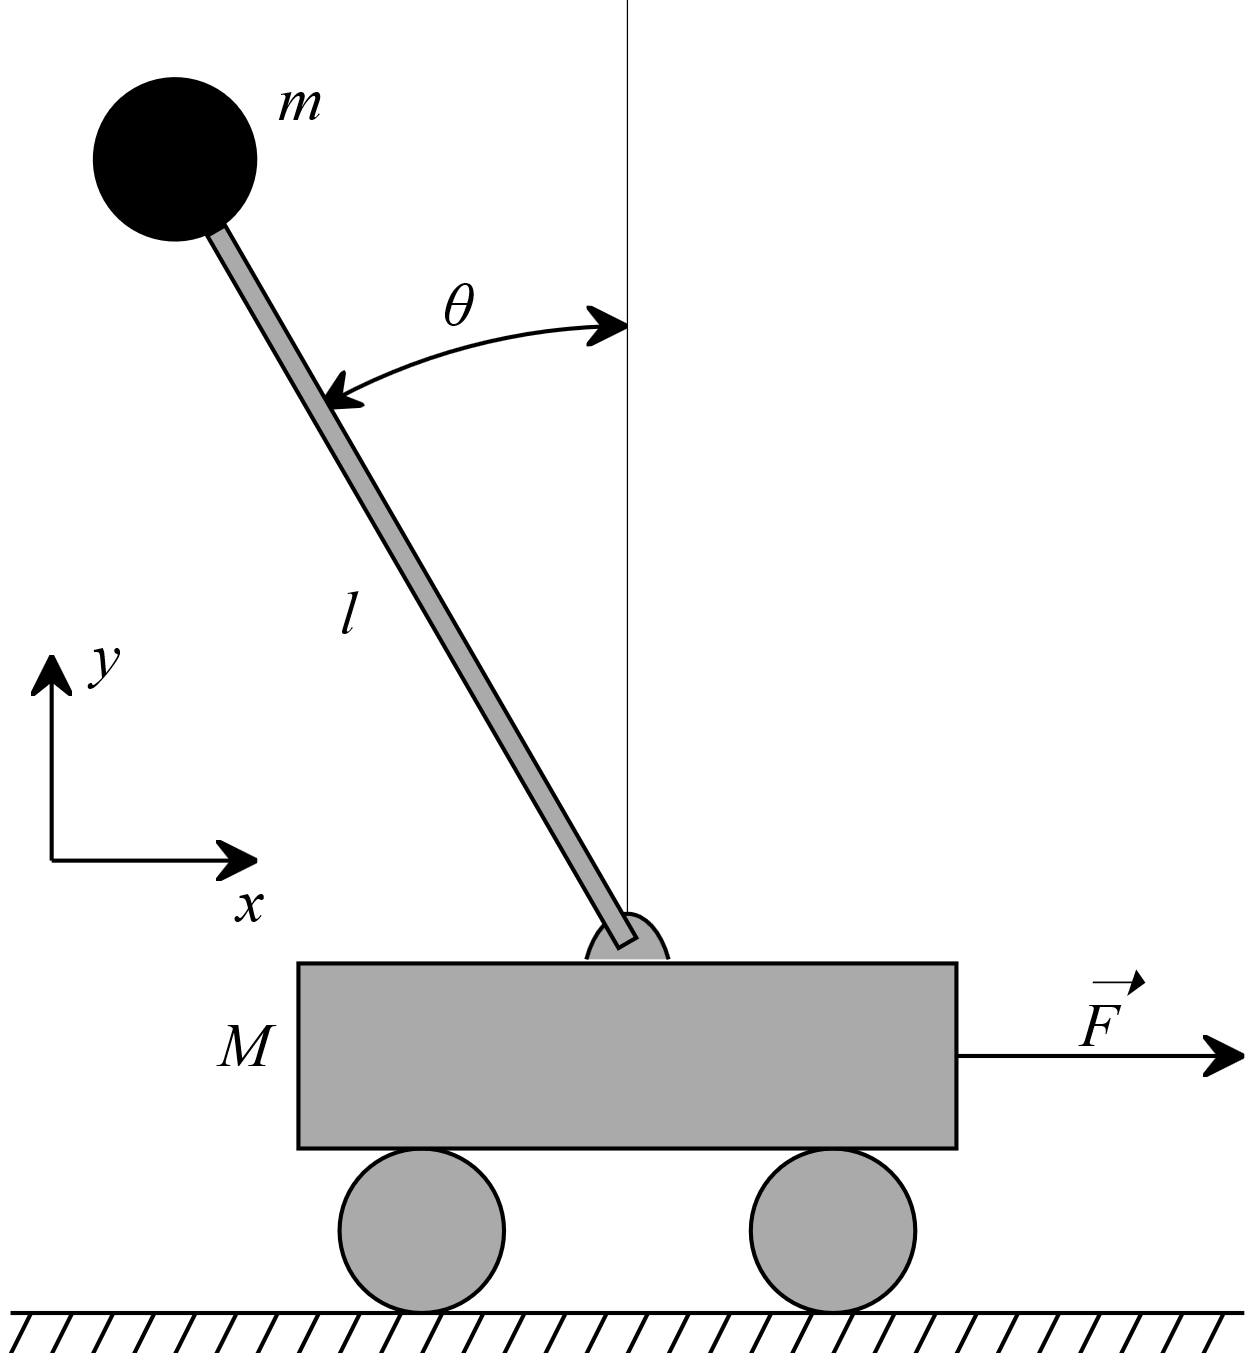
\includegraphics[trim = 0em 0em 0em 0em, clip, width=0.4\textwidth]{cart-pendulum.png}%
}%
\caption[{[Selection of Control Problem]: Inverted Pendulum on Cart}]%
        {{[Selection of Control Problem]: Inverted Pendulum on Cart~%
          \cite{REF:online:wikipedia:invertedPendulum:physicalModel}%
          \label{FIG:preliminaryDecisions:selectionControlProblem:invertedPendulum}%          
        }}%
\end{figure}
\vspace*{\fill}




\clearpage




The motoring device is used in such a setup to provide counterforces to the mounted end of the pendulum.
These counterforces are intended to ultimately return the top of the pendulum to its inverted {\fns(standing)} position.

For the actuator to successfully perform these actions, a controller {\fns(calculation device)} is required.
The controller, with the assistance of sensory data, is able to dynamically calculate {\fns(in real time)} 
the exact forces needed to reestablish the positioning of the pendulum to a standing equilibrium.
The controller then communicates the magnitude and direction of these forces to the motoring device 
which actuates the forces in the physical space.
This in turn changes the state of the system, 
requiring that the controller continually recalculate the forces needed to return to equilibrium.

This problem may be further complicated by implementing trajectory control,
in which the operator may command the device to move to one or more different locations.
In such a scenario, the device must maintain its control of the balance of the inverted pendulum
during and after moving.




\subsection{Two-Wheeled Robot}
\label{SEC:preliminaryDecisions:selectionControlProblem:twoWheeledRobot}

The two-wheeled robot is a special case of the inverted pendulum model.
In this case, the inverted pendulum model is reduced to only the pendulum and the wheels.
The entirety of the robot hardware forms the pendulum, and
the pendulum is coupled directly to the wheels.

One such device is depicted in Figure~%
\ref{FIG:preliminaryDecisions:selectionControlProblem:twoWheeledRobot}.
In this case, the robot is being used in a medical application.
The significance of the two-wheeled robot is not related to any one application; rather
its ability to balance allows the added inclusion of top-heavy architectures in design options.

The robot has two wheels, 
each of which is coupled to an individual motoring device {\fns(included in the robot hardware)}.
The motoring devices are able to act independently; therefore,
the device is capable of turning and moving across a two-dimensional plane.
This transition from one shaft to two shafts creates additional complexity in the system
which must be considered in the design of the controller.




\clearpage




\vspace*{\fill}
\begin{figure}[H]
\centering%
\fbox{%
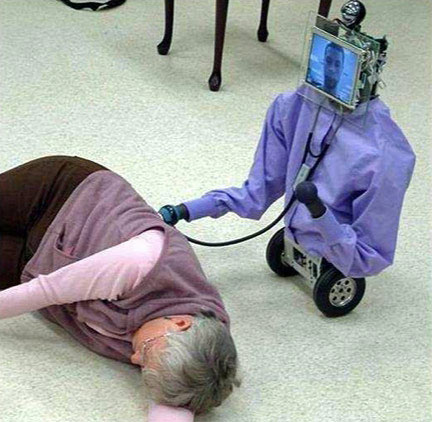
\includegraphics[trim = 0em 0em 0em 0em, clip, width=0.7\textwidth]{two-wheeled-robot-ubot-5.jpg}%
}%
\caption[{[Selection of Control Problem]: Two Wheeled Robot}]%
        {{[Selection of Control Problem]: Two Wheeled Robot~%
          \cite{REF:online:twoWheeledRobot:examplePhoto}%
          \label{FIG:preliminaryDecisions:selectionControlProblem:twoWheeledRobot}%
        }}
\end{figure}
\vspace*{\fill}




\clearpage




\end{document}











% !TEX spellcheck = English (United States) (Aspell)
% !TEX TS-program = arara
%  arara: lmkclean
%  arara: pdflatex: {   draft: yes, options: '-file-line-error -halt-on-error' }
%  arara: biber
%  arara: pdflatex: {   draft: yes, options: '-file-line-error -halt-on-error' }
%  arara: pdflatex: { synctex: yes, options: '-file-line-error -halt-on-error' }
%  arara: lmkclean
\documentclass[crop=false,float=true,class=scrreprt]{standalone}

\providecommand{\main}{../../..}
% Preamble
 \input{\main/Subfiles/0-Preamble/1-packages.tex}

 \input{\main/Subfiles/0-Preamble/2-userInput-graphicsPath.tex}

 \input{\main/Subfiles/0-Preamble/3-pageLayout.tex}


% Watermark
 \input{\main/Subfiles/0-Preamble/watermark.tex}

% Floats:
 \input{\main/Subfiles/0-Preamble/floatConfig.tex}
%\input{\main/Subfiles/0-Preamble/sectionNumberIncludedInFloatCounter.tex}

% Commands:
 \input{\main/Subfiles/0-Preamble/commonCommands.tex}
 \input{\main/Subfiles/0-Preamble/allsubsSections.tex}
 \input{\main/Subfiles/0-Preamble/changePageSize.tex}

% Bug Fixes:
 \input{\main/Subfiles/0-Preamble/nociteFix.tex}
  % Preamble [document configuration]

\begin{document}




\section{Selection of Hardware}
\label{SEC:preliminaryDecisions:selectHardware}

% !TEX TS-program = arara
%  arara: lmkclean
%  arara: pdflatex: {   draft: yes, options: '-file-line-error -halt-on-error' }
%  arara: biber
%  arara: pdflatex: {   draft: yes, options: '-file-line-error -halt-on-error' }
%  arara: pdflatex: { synctex: yes, options: '-file-line-error -halt-on-error' }
%  arara: lmkclean
\documentclass[crop=false,float=true,class=scrreprt]{standalone}

\providecommand{\main}{../../..}
\input{\main/Subfiles/0-Preamble/0-Preamble.tex}  % Preamble [document configuration]

\begin{document}




The test platform consists of the designated hardware,
{\fns[\tif{MinSeg M2V3 two-wheeled robot, see Section~\ref{SEC:preliminaryDecisions:selectHardware:minseg}}]},
and the designated development PC,
{\fns[\tif{see Section~\ref{SEC:preliminaryDecisions:selectHardware:developmentPC}}]}.
To interface with the hardware,
a Simulink model and a hierarchy of Matlab subscripts were created.

The Simulink model is capable of: 

\begin{itemize}[leftmargin=*, label=$\vcenter{\hbox{\tiny$\bullet$}}$, itemsep=-1em]

\item Acting as an algorithm with which to program the hardware, such that it may:
      \vspace*{-1em}
      \begin{itemize}[leftmargin=*, label=$\cdot$, itemsep=-1em]
      
      \item Process
      
      \item Actuate
      
      \item Communicate
      
      \end{itemize}

\item Simulate an equivalent model of "the hardware when loaded with the same algorithm".

\end{itemize}


The Matlab script hierarchy is capable of:

\begin{itemize}[leftmargin=*, label=$\vcenter{\hbox{\tiny$\bullet$}}$, itemsep=-1em]

\item Initialize model parameters.

\item Reconfigure model subsystems.

\item Initialize a build or simulate event.

\item Initialize a read or write event.

\item Post-process raw read data.

\item Save processed read data as well as other configuration data.

\item Plot processed read data.

\end{itemize}




\clearpage 




\end{document}











% !TEX spellcheck = English (United States) (Aspell)
% !TEX TS-program = arara
%  arara: lmkclean
%  arara: pdflatex: {   draft: yes, options: '-file-line-error -halt-on-error' }
%  arara: biber
%  arara: pdflatex: {   draft: yes, options: '-file-line-error -halt-on-error' }
%  arara: pdflatex: { synctex: yes, options: '-file-line-error -halt-on-error' }
%  arara: lmkclean
\documentclass[crop=false,float=true,class=scrreprt]{standalone}

\providecommand{\main}{../../../..}
\input{\main/Subfiles/0-Preamble/0-Preamble.tex}  % Preamble [document configuration]

\begin{document}


%\addtocontents{toc}{\string\setcounter{tocdepth}{2}}
%\startcontents[preliminaryDecisions:selectionHardware]

%\renewcommand{\sectionedEquation}{\thesubsection--\arabic{equation}}
%\counterwithin*{equation}{subsection}




\subsection{MinSeg M2V3 Two-Wheeled Robot}
\label{SEC:preliminaryDecisions:selectHardware:minseg}


\iffalse


\singlespacing%
\printcontents[preliminaryDecisions:selectionHardware]{}{1}{%
  \addtocontents{ptc}{\string\setcounter{tocdepth}{5}}%
% 
  \subsection*{List of Contents}%
% \addcontentsline{toc}{subsection}{List of Contents}%
  }%
\doublespacing%
\clearpage


\fi


\input{\main/Subfiles/2-Main/02-preliminaryDecisions/02-selectHardware/01-minseg/00-root.tex}
\input{\main/Subfiles/2-Main/02-preliminaryDecisions/02-selectHardware/01-minseg/components.tex}
\input{\main/Subfiles/2-Main/02-preliminaryDecisions/02-selectHardware/01-minseg/arduino.tex}
\input{\main/Subfiles/2-Main/02-preliminaryDecisions/02-selectHardware/01-minseg/bluetoothModule.tex}
\input{\main/Subfiles/2-Main/02-preliminaryDecisions/02-selectHardware/01-minseg/powerSource.tex}
\input{\main/Subfiles/2-Main/02-preliminaryDecisions/02-selectHardware/01-minseg/motorDriver.tex}
\input{\main/Subfiles/2-Main/02-preliminaryDecisions/02-selectHardware/01-minseg/motorGearboxEncoder.tex}
\input{\main/Subfiles/2-Main/02-preliminaryDecisions/02-selectHardware/01-minseg/gyroAccel.tex}
\input{\main/Subfiles/2-Main/02-preliminaryDecisions/02-selectHardware/01-minseg/arduinoInterfaces.tex}




%\renewcommand{\sectionedEquation}{\thesection--\arabic{equation}}
%\counterwithout*{equation}{subsection}

%\stopcontents[preliminaryDecisions:selectionHardware]
%\addtocontents{toc}{\string\setcounter{tocdepth}{1}}



\end{document}











% !TEX spellcheck = English (United States) (Aspell)
% !TEX TS-program = arara
%  arara: lmkclean
%  arara: pdflatex: {   draft: yes, options: '-file-line-error -halt-on-error' }
%  arara: biber
%  arara: pdflatex: {   draft: yes, options: '-file-line-error -halt-on-error' }
%  arara: pdflatex: { synctex: yes, options: '-file-line-error -halt-on-error' }
%  arara: lmkclean
\documentclass[crop=false,float=true,class=scrreprt]{standalone}

\providecommand{\main}{../../../..}
\input{\main/Subfiles/0-Preamble/0-Preamble.tex}  % Preamble [document configuration]

\begin{document}




\subsection{Development PC}
\label{SEC:preliminaryDecisions:selectHardware:developmentPC}

Designations pertaining to the development PC
with respect to the test platform
are exhibited in Table~%
\ref{TAB:testPlatform:developmentPC}.


\vspace*{\fill}
\begin{table}[H]
\centering%
\small%
\caption[{[Selection of Compatible HW \& SW]: Development PC Specifications}]%
        {{[Selection of Compatible HW \& SW]: Development PC Specifications~%
           \cite{REF:online:powerstream:batteryDrainage}%
           \label{TAB:testPlatform:developmentPC}%
        }}%
\begin{tabular}{ | l | c | }                                                                                 \hline & \\[-2.0em]
\tbf{Hardware}                                       & \tbf{Version}                              \\[+0.0em] \hline & \\[-2.0em]
PC                                                   & 2015 Macbook Pro 
                                                       \cite{REF:online:everymac:macbookpro:2015} \\[+0.0em] \hline
\mc{2}{c}{}                                                                                       \\[-1.0em] \hline   \\[-2.0em]
\tbf{Software}                                       & \tbf{Version}                              \\[+0.0em] \hline & \\[-2.0em]
Operating System (OS)                                & macOS 10.12.5                              \\[+0.0em] \hline & \\[-2.0em]
%%
\begin{tabular}{@{}l@{}}
Mathworks Software Suite                             \\
$\cdot$ \tif{MATLAB}                                 \\
$\cdot$ \tif{Simulink}                               \\
$\cdot$ \tif{Control System Toolbox}                 \\
$\cdot$ \tif{DSP System Toolbox}                     \\
$\cdot$ \tif{Instrument Control Toolbox}             \\
$\cdot$ \tif{MATLAB Coder}                           \\
$\cdot$ \tif{Simulink Coder}                         \\
$\cdot$ \tif{Simulink Desktop Real-Time}             \\[+1em]
$\cdot$
\tif{Matlab   Support Package for Arduino Hardware}  \\
$\cdot$
\tif{Simulink Support Package for Arduino Hardware}  \\
\end{tabular}                                        &
\begin{tabular}{@{}c@{}}
r2017a                                               \\
-                                                    \\
-                                                    \\
-                                                    \\
-                                                    \\
-                                                    \\
-                                                    \\
-                                                    \\
-                                                    \\[+1em]
17.1.0                                               \\
17.1.0                                               \\
\end{tabular}                                                                                     \\[+0.0em] \hline & \\[-2.0em]
%%
Xcode
\hspace*{\fill}{\fns
[\tif{A Mathworks (macOS)-Supported Compiler
\cite{REF:online:mathworks:supportedCompilers}.}]}    & 7.3.1                                      \\[+0.0em] \hline & \\[-2.0em]
%%
\begin{tabular}{@{}l@{}}
Rensselaer Arduino Support Package Library (RASPLib)
\hspace*{+4em}                                       \\
\hspace*{\fill}{\fns
[\tif{A third-party Simulink Support Package for MinSeg Hardware
\cite{REF:online:hurst:minsegDrivers}.}]}    
\end{tabular}                                        &
\begin{tabular}{@{}c@{}}
1.1                                                  \\
\end{tabular}                                                                                     \\[+0.0em] \hline
\end{tabular}
\end{table}
\vspace*{\fill}




\clearpage




\subsubsection{Designated PC}
\label{SEC:preliminaryDecisions:selectionHardware:developmentPC:pc}

A 2015 Macbook Pro PC was selected as the designated development PC,
as this was available to the researcher
without the need to request additional funding.




\vspace{+2em}




\subsubsection{Designated Operating System}
\label{SEC:preliminaryDecisions:selectionHardware:developmentPC:os}

macOS was selected as the designated operating system,
as this was the only operating system installed on the designated PC.
{\fns(\tif{Version 10.12.5 was the most up to date version at the time of research.})}

\tbf{Alternative Operating System Compatibility}

Although the macOS operating system was used,
alternative operating systems {\fns(\tif{Windows and/or Linux})} would be equally acceptable.

Such a transition would primarily require an alternative Mathworks-supported compiler 
 \cite{REF:online:mathworks:supportedCompilers}
which would be compatible with the new operating system.
Slight alterations to the method of determining the test platform serial communication channel\iffalse, 
as described in Section~%
\ref{SEC:testPlatform:determiningSerialCommunicationChannel?}\fi
would also be required.

It is not expected that such a transition would be prohibitively difficult.




\clearpage




\subsubsection{Designated Hardware-Interfacing Software}
\label{SEC:preliminaryDecisions:selectionHardware:developmentPC:mathworks}

The Mathworks Software Suite was selected as the designated hardware-interfacing software due to:

\vspace{-0em}
\begin{itemize}[leftmargin=*]

\item Its first-party support for programming real-time hardware.

\item Its first-party support for simulating real-time hardware.

\item Its first-party driver support for Arduino-brand microcontrollers.

\item Its third-party driver support for the MinSeg.

\item Its first-party support for serial communication with hardware in real-time.

\item Its relatively user-friendly language and interfaces.

\item Its relative commonality among students and academic institutions.\\[+0.25em]
      \hspace*{\fill}{\fns$
      \begin{bmatrix*}[r]
      \text{\tif{The software environment was already relatively familiar to}}\\
      \text{\tif{the author and to the advising professor prior to performing this study.}}
      \end{bmatrix*}
      $}

\item Its relatively affordable cost. 
      \hspace*{\fill}{\fns[\tif{With respect to students and academic institutions.} \raisebox{-0.75ex}{\textasciitilde}\tif{\$150}]}.

\end{itemize}
\vspace{-1em}




\iffalse

\subsubsubsection{Supported Compiler}
\label{SEC:preliminaryDecisions:selectionHardware:developmentPC:mathworks:compiler}




\subsubsubsection{First-Party Support Packages}
\label{SEC:preliminaryDecisions:selectionHardware:developmentPC:mathworks:arduinoSupport}




\subsubsubsection{Third-Party Support Packages}
\label{SEC:preliminaryDecisions:selectionHardware:developmentPC:mathworks:minsegSupport}

who

where

how





\clearpage




\subsubsection{Arduino Interfacing}
\label{SEC:preliminaryDecisions:selectionHardware:developmentPC:arduinoInterfacing}




\subsubsubsection{Programming}




\subsubsubsection{Serial Communication}




\fi




\clearpage



\end{document}
















\end{document}











% !TEX spellcheck = English (United States) (Aspell)
% !TEX TS-program = arara
%  arara: lmkclean
%  arara: pdflatex: {   draft: yes, options: '-file-line-error -halt-on-error' }
% !arara: bibtex
%  arara: biber
%  arara: pdflatex: {   draft: yes, options: '-file-line-error -halt-on-error' }
%  arara: pdflatex: { synctex: yes, options: '-file-line-error -halt-on-error' }
%  arara: lmkclean
\documentclass[crop=false,float=true,class=scrreprt]{standalone}

\providecommand{\main}{../../..}
% Preamble
 \input{\main/Subfiles/0-Preamble/1-packages.tex}

 \input{\main/Subfiles/0-Preamble/2-userInput-graphicsPath.tex}

 \input{\main/Subfiles/0-Preamble/3-pageLayout.tex}


% Watermark
 \input{\main/Subfiles/0-Preamble/watermark.tex}

% Floats:
 \input{\main/Subfiles/0-Preamble/floatConfig.tex}
%\input{\main/Subfiles/0-Preamble/sectionNumberIncludedInFloatCounter.tex}

% Commands:
 \input{\main/Subfiles/0-Preamble/commonCommands.tex}
 \input{\main/Subfiles/0-Preamble/allsubsSections.tex}
 \input{\main/Subfiles/0-Preamble/changePageSize.tex}

% Bug Fixes:
 \input{\main/Subfiles/0-Preamble/nociteFix.tex}
  % Preamble [document configuration]

\begin{document}




\section{Selection of a Hardware Model}
\label{SEC:preliminaryDecisions:selectionHardwareModel}

The physical plant model developed in
\textcite{REF:online:2009-yamamoto}
was used, due to:

\begin{itemize}[leftmargin=*]

\item Use of state variables involving:
\begin{itemize}[leftmargin=*]

  \item Body pitch angle $\alpha$
  
  \item Body yaw angle $\Psi$
  
  \item Wheel angle $\theta$

\end{itemize} 

\item Existing familiarity of the work by the advising professor.

\item Existing knowledge of methods to measure nonintuitive model parameters by the advising professor.

\end{itemize}


The physical plant model is discussed in greater detail in Chapter~%
\ref{SEC:hwePlantDynamicsModel}.




\clearpage





\end{document}











% !TEX spellcheck = English (United States) (Aspell)
% !TEX TS-program = arara
%  arara: lmkclean
% !arara: pdflatex: {   draft: yes, options: '-file-line-error -halt-on-error' }
% !arara: bibtex
% !arara: biber
%  arara: pdflatex: {   draft: yes, options: '-file-line-error -halt-on-error' }
%  arara: pdflatex: { synctex: yes, options: '-file-line-error -halt-on-error' }
%  arara: lmkclean
\documentclass[crop=false,float=true,class=scrreprt]{standalone}

\providecommand{\main}{../../..}
% Preamble
 \input{\main/Subfiles/0-Preamble/1-packages.tex}

 \input{\main/Subfiles/0-Preamble/2-userInput-graphicsPath.tex}

 \input{\main/Subfiles/0-Preamble/3-pageLayout.tex}


% Watermark
 \input{\main/Subfiles/0-Preamble/watermark.tex}

% Floats:
 \input{\main/Subfiles/0-Preamble/floatConfig.tex}
%\input{\main/Subfiles/0-Preamble/sectionNumberIncludedInFloatCounter.tex}

% Commands:
 \input{\main/Subfiles/0-Preamble/commonCommands.tex}
 \input{\main/Subfiles/0-Preamble/allsubsSections.tex}
 \input{\main/Subfiles/0-Preamble/changePageSize.tex}

% Bug Fixes:
 \input{\main/Subfiles/0-Preamble/nociteFix.tex}
  % Preamble [document configuration]

\begin{document}




\section{Selection of Controller Design}
\label{SEC:preliminaryDecisions:selectionControllerDesign}


Since pole-placement methods had been researched relatively recently 
under the advising professor,
optimal control techniques were researched.

This is discussed in greater detail in Section~%
\ref{SEC:controllerDesign}.




\clearpage




\end{document}











% !TEX TS-program = arara
%  arara: lmkclean
%  arara: pdflatex: {   draft: yes, options: '-file-line-error -halt-on-error' }
%  arara: biber
%  arara: pdflatex: {   draft: yes, options: '-file-line-error -halt-on-error' }
%  arara: pdflatex: { synctex: yes, options: '-file-line-error -halt-on-error' }
%  arara: lmkclean
\documentclass[crop=false,float=true,class=scrreprt]{standalone}

\providecommand{\main}{../..}
% Preamble
 \input{\main/Subfiles/0-Preamble/1-packages.tex}

 \input{\main/Subfiles/0-Preamble/2-userInput-graphicsPath.tex}

 \input{\main/Subfiles/0-Preamble/3-pageLayout.tex}


% Watermark
 \input{\main/Subfiles/0-Preamble/watermark.tex}

% Floats:
 \input{\main/Subfiles/0-Preamble/floatConfig.tex}
%\input{\main/Subfiles/0-Preamble/sectionNumberIncludedInFloatCounter.tex}

% Commands:
 \input{\main/Subfiles/0-Preamble/commonCommands.tex}
 \input{\main/Subfiles/0-Preamble/allsubsSections.tex}
 \input{\main/Subfiles/0-Preamble/changePageSize.tex}

% Bug Fixes:
 \input{\main/Subfiles/0-Preamble/nociteFix.tex}
  % Preamble [document configuration]

\begin{document}




\printbibliography[segment=\therefsegment, heading=subbibnumbered, title={References}]




\clearpage 




\end{document}















%\renewcommand{\sectionedEquation}{\thesection--\arabic{equation}}
%\counterwithout*{equation}{subsection}

\stopcontents[preliminaryDecisions]
%\addtocontents{toc}{\string\setcounter{tocdepth}{1}}




\end{document}










  %\addtocontents{toc}{\string\clearpage}
 % !TEX spellcheck = English (United States) (Aspell)
% !TEX TS-program = arara
%  arara: lmkclean
%  arara: pdflatex: {   draft: yes, options: '-file-line-error -halt-on-error' }
%  arara: biber
%  arara: pdflatex: {   draft: yes, options: '-file-line-error -halt-on-error' }
%  arara: pdflatex: { synctex: yes, options: '-file-line-error -halt-on-error' }
%  arara: lmkclean
\documentclass[crop=false,float=true,class=scrreprt]{standalone}

\providecommand{\main}{../..}
% Preamble
 % meta tools
\usepackage{standalone}                 % allows for independent runs of subfiles. [includes currfile].
                                        % IMPORTANT: [realmainfile] option of currfile requires compiler option -recorder to be active.
                                        % IMPORTANT: standalone loads currfile package without options.  To configure currfile options:
                                        %            place them in \documentclass[options](standalone) options. 
                                        %      NOTE: Loading the currfile package with options will clash with the standalone package.
\usepackage{etoolbox}                   % allows if/else statements in code. [required for: standalone+nocite fix, equation numbering.]

% math
\usepackage{mathtools}                  % includes amsmath, supplements it.
\usepackage{subdepth}                   % allows manual vertical alignment for misaligned subscripts.

% font
\newcommand{\xLanguage}{american}       % do not remove: used in multiple locations.
\usepackage[\xLanguage]{babel}          % hyphenates words correctly, based on document language. [\xlanguage is defined immediately above.]
\usepackage{amssymb}                    % symbols. [permits use of \bigstar].
%\usepackage{mathptmx}                  % times new roman font. totally lame, but required by EB. [supercedes 'times' package].
\usepackage[T1]{fontenc}                % improves pdf reader's ability to copy    atypical text characters from output pdf file.
\usepackage[latin1]{inputenc}           % improves tex editor's ability to compile atypical text characters into output pdf file from tex file.

%\usepackage{verbatim}                  % [superceded by listings] improves verbatim environment. [includes comment package].
\usepackage{listings}                   % improved version of verbatim. imports script languages (with syntax coloring).

\usepackage{color}                      % color commands.
\usepackage[dvipsnames]{xcolor}         % additional color commands.

\usepackage{soul}                       % strikethrough commands.
\usepackage{transparent}                % transparent objects/font.

% layout: page/spacing/headings
\usepackage{geometry}                   % margin/page layout settings.
\usepackage{changepage}                 % allows adjustwidth, for figures larger than the margins.
\usepackage{pdflscape}                  % landscape page layout.
\usepackage{scrlayer-scrpage}           % improved header commands. [supercedes `fancyhdr' package].

\usepackage{eso-pic}                    % watermarks. [xwatermark is not compatible with scrpage. draftwatermark is not included with Tex Live.]

 \usepackage{setspace}                  % line spacing (allows \doublespacing). <-- not for urithesis
%\usepackage{parskip}                   % [superceded by KOMA]. tidies spacing. 

%\usepackage{titlesec}                  % [superceded by KOMA]. change style of all page      headers, etc.
%\usepackage{sectsty}                   % [superceded by KOMA]. change style of all sectional headers, etc.
\usepackage[toc,page]{appendix}         % appendices. [toc adds Appendices to TOC, page adds a page listed Appendices in the document.]

% references
\usepackage{chngcntr}                   % allows changes mid-document to section depth of equation counter reset.
\usepackage[titles]{tocloft}            % allows new lists such as \listofequations and \listoflistings.
                                        % Note: titles option permits header on table of contents and list of figures/tables/etc pages.
\usepackage{titletoc}                   % allows sub-[tables of contents]. allows increased margin between numbers and labels in toc.
                                        % IMPORTANT: [breaks \section* commands. use \setcounter{secnumdepth}{0} instead.]

% floats: figures/tables/lists
\usepackage{float}                      % improves floating objects (graphics/tables).

\usepackage{graphics}
\usepackage{graphicx}                   % graphics incorporation.
\usepackage{wrapfig}                    % allows text wrapping of figures.
\usepackage{subcaption}                 % allow captions with the subcaption command. [automatically loads caption package.]

\usepackage{tabu}                       % improved table commands.
\usepackage{longtable}                  % allows multipage tables.
\usepackage{multirow}                   % multirow command.
\usepackage{bigstrut}                   % bigstrut command. adds slight space up [t], down [b], or both. try next to \hline.
\usepackage{booktabs}                   % improved hline spacing commands in tables.

\usepackage{enumitem}                   % improved alterations to indent in enumerate/itemize. allows enumerate counter nesting.

% references
\usepackage{csquotes}                   % required for biblatex when using babel.
\usepackage{xpatch}                     % required for ieee-style @online no-date fix.

\usepackage[ backend      = biber       % supercedes bibtex
           , sorting      = none        % none: entries appear in order of \cite use
           , refsegment   = chapter     % restart numbering at beginning of each chapter
           , defernumbers = true,       % required for added global bibliography
           , style        = ieee        % ieee style
%          , doi          = false       % false for ieee style?
%          , isbn         = false       % false for ieee style?
           , citestyle    = numeric,    % \cite{REF:A, REF:B} => [1,2] instead of the default => [1], [2]
           , url          = true   ]
            {biblatex}                  % bibliographies (supercedes bibtex, biber, ...)

% hyperref                              % IMPORTANT: Always load hyperref last. It tends to break other packages when loaded first.
\usepackage[ hidelinks
           , linktoc   = all     ]
           {hyperref}                   % hyperlinks.












 %Setup Up Paths for Figures
\graphicspath{ %
             {\main/Figures/}                                % Directories for master file
             {\main/Figures/01-Intro/TitlePage/} 
             %
             {\main/Figures/02-Main/}
             {\main/Figures/02-Main/Verification/}
             %
             %
             }



 % Page size, margin, and header/footer settings:

% Enable "showframe" when editing margins
%\usepackage{showframe}                                            % Uncomment this to display header/footer/margins outlines.

% General margin settings:
 \newlength{\xhmargin   } \setlength  {\xhmargin   }{+1.000in    }
 \newlength{\xlmargin   } \setlength  {\xlmargin   }{\xhmargin   }
%                         \addtolength{\xlmargin   }{+0.500in    } % Include this row for additional margin for paper binding.
 \newlength{\xrmargin   } \setlength  {\xrmargin   }{\xhmargin   }
  
 \newlength{\xtmargin   } \setlength  {\xtmargin   }{+1.000in    } % Actual  tmargin = [\xtmargin - \xheadheight] = [0.500in] 
 \newlength{\xbmargin   } \setlength  {\xbmargin   }{+1.000in    } % Actual  bmargin = [\xbmargin - \xfootskip  ] = [0.500in] 

% Header  margin settings:
 \newlength{\xheadheight} \setlength  {\xheadheight}{+0.500in    } % May need to adjust tmargin in addition to this.
 \newlength{\xheadsep   } \setlength  {\xheadsep   }{+1.000em    }

% Footer  margin settings:
 \newlength{\xfootheight} \setlength  {\xfootheight}{+0.500in    } % May need to adjust bmargin in addition to this.
 \newlength{\xfootskip  } \setlength  {\xfootskip  }{\xfootheight} % Actual footskip = [\xfootheight - 1em + desired footsep] = [0.500in]
                          \addtolength{\xfootskip  }{-1.000em    } % <-- do not edit
                          \addtolength{\xfootskip  }{+1.000em    } % <-- do     edit: desired footsep



\KOMAoptions{headheight    = \xheadheight,
             footheight    = \xfootheight,
             DIV           = current,
             fontsize      = 10pt,
             parskip       = half-,
             toc           = chapterentrydotfill,
           % headings      = small,
           % headings      = openany,
             headings      = twolinechapter}

\geometry{letterpaper,
          tmargin       = \xtmargin,
          bmargin       = \xbmargin,
          lmargin       = \xlmargin,
          rmargin       = \xrmargin,
          headsep       = \xheadsep,
          footskip      = \xfootskip}

\savegeometry{default}




% Initialize double-spacing
\doublespacing




% Section headings

%\setkomafont{sectioning}   {\bfseries}
%\setkomafont{chapter}      {\nms}
%\setkomafont{section}      {\nms}
%\setkomafont{subsection}   {\nms}
%\setkomafont{subsubsection}{\nms}
%\setkomafont{paragraph}    {\nms}
%\setkomafont{subparagraph} {\nms}

\RedeclareSectionCommands[font       =  \nms,
                          beforeskip =  0pt,            % vspace before  chapter heading
                          innerskip  = -\parskip,       % vspace between chapter heading lines
                          afterskip  =  1\baselineskip] % vspace after   chapter heading
                         {chapter}
                         
\RedeclareSectionCommands[font       =  \nms,
                          afterskip  =  0.001em] % 0em puts the text inline with the heading. >.<
                          {section,subsection,subsubsection,paragraph,subparagraph}

% Make the word Chapter uppercase (but not the section heading label)
% Add a visible horizontal line
\renewcommand*{\chapterformat}{%
  \MakeUppercase{\chapappifchapterprefix{\nobreakspace}}\thechapter\autodot%
    \IfUsePrefixLine{%
        \par\nobreak\vspace*{-\parskip}\vspace*{-.6\baselineskip}%
        \rule{0.75\textwidth}{.5pt}%
}{\enskip}}%


\renewcommand\raggedchapter{\centering}


% Initialize headers and footers

\setkomafont{pageheadfoot}{\normalfont\normalcolor}

% Header: Center:
\chead{\fns}

% Footer: Center:
\cfoot{\thepage}

% Footer: Right-Side:
\ofoot{\fns}

% Header/footer enable/disable switch
\newpairofpagestyles{trueempty}{}
%  Enable: \pagestyle{scrheadings} [this is the default.]
% Disable: \pagestyle{trueempty}




% Watermark
 % Initialize watermark

\iffalse % <-- [ \iffalse: disabled | \iftrue: enabled ]
\AddToShipoutPictureFG{ 

\raisebox{.5\paperheight}{
\begin{minipage}[c][\paperheight][c]{\paperwidth}
\centering
\rotatebox[origin=c]{45}{ 
\scalebox{15}{ 
\transparent{0.35} \color{gray} D\sc{raft}
} } 
\end{minipage}
}

}
\fi


































% Floats:
 % Names of [float] and List of [float]

% Allow multiline captions to be centered.
\captionsetup{format=plain, justification=centering}




%-List of Contents
\expandafter\addto\csname captions\xLanguage\endcsname{% This line is needed when using the babel package.
  \renewcommand{\contentsname}{Table of Contents}%      % \xLanguage is defined in [1-packages.tex] near babel package.
                                                      }%  Renames Contents to List of Contents      

%-List of Code Listings
\renewcommand{\lstlistingname}    {Code Listing}              % Rename ``Listing'' floats to ``Code Listing'' floats.
\renewcommand{\lstlistlistingname}{List of \lstlistingname s \vspace{+0.40em}}








% Settings for importing scripts [listings package]


\lstset{ %
   backgroundcolor  = \color{white},     % choose the background color; you must add \usepackage{color} or \usepackage{xcolor}
   basicstyle       = \footnotesize,     % the size of the fonts that are used for the code
   breakatwhitespace= false,             % sets if automatic breaks should only happen at whitespace
   breaklines       = true,              % sets automatic line breaking
   captionpos       = tb,                % sets the caption-position
   commentstyle     = \color{Green},     % comment style
   deletekeywords   = {...},             % if you want to delete keywords from the given language
   escapeinside     = {\%*}{*)},         % if you want to add LaTeX within your code
   extendedchars    = true,              % lets you use non-ASCII characters; for 8-bits encodings only, does not work with UTF-8
   frame            = single,            % adds a frame around the code
   keepspaces       = true,              % keeps spaces in text, 
                                         %   useful for keeping indentation of code (possibly needs columns=flexible)
   keywordstyle     = \color{blue},      % keyword style
   language         = Matlab,            % the language of the code
   morekeywords     = {*,...},           % if you want to add more keywords to the set
   numbers          = left,              % where to put the line-numbers; possible values are (none, left, right)
   numbersep        = 5pt,               % how far the line-numbers are from the code
   numberstyle      = \tiny\color{gray}, % the style that is used for the line-numbers
   rulecolor        = \color{black},     % if not set, the frame-color may be changed on line-breaks within 
                                         %   not-black text (e.g. comments (green here))
   showspaces       = false,             % show spaces everywhere adding particular underscores; it overrides 'showstringspaces'
   showstringspaces = false,             % underline spaces within strings only
   showtabs         = false,             % show tabs within strings adding particular underscores
   stepnumber       = 1,                 % the step between two line-numbers. If it's 1, each line will be numbered
   stringstyle      = \color{purple},    % string literal style
   tabsize          = 2,                 % sets default tabsize to 2 spaces
   title            = \lstname           % show the filename of files included with \lstinputlisting; also try caption 
                                         %   instead of title
}















%% Sectioned Float Counters:

% Required Packages:
% - chngcntr
% - etoolbox
% - listings
% - titletoc


% Save a copy of the original float counters.
\let\xtheequationOriginal\theequation
\let\xthefigureOriginal\thefigure
\let\xthetableOriginal\thetable
\let\xthelstlistingOriginal\thelstlisting




% Command: Sectioned Counter

\newcommand{\sectionedCounter}     [1]
  % Input #1: section, subsection, subsubsection, paragraph, subparagraph, or \determineSection
  %
  %-This command configures all float counters to reset when switching to 
  %   a new section at (or above) a user-specified depth.
  % Reuse of the command overwrites the previous reset flags.
  %
  %-This command prepends all float counters with the current section number 
  %  (at the user-specified depth).
{
  \counterwithout*{equation}  {section} 
  \counterwithout*{figure}    {section}
  \counterwithout*{table}     {section}
  \counterwithout*{lstlisting}{section}
    
  \counterwithout*{equation}  {subsection} 
  \counterwithout*{figure}    {subsection}
  \counterwithout*{table}     {subsection}
  \counterwithout*{lstlisting}{subsection}
    
  \counterwithout*{equation}  {subsubsection} 
  \counterwithout*{figure}    {subsubsection}
  \counterwithout*{table}     {subsubsection}
  \counterwithout*{lstlisting}{subsubsection}
    
  \counterwithout*{equation}  {paragraph} 
  \counterwithout*{figure}    {paragraph}
  \counterwithout*{table}     {paragraph}
  \counterwithout*{lstlisting}{paragraph}
    
  \counterwithout*{equation}  {subparagraph} 
  \counterwithout*{figure}    {subparagraph}
  \counterwithout*{table}     {subparagraph}
  \counterwithout*{lstlisting}{subparagraph}

  \counterwithin*{equation}  {#1}   % Reset counter whenever there is a new \section
  \counterwithin*{figure}    {#1}
  \counterwithin*{table}     {#1}
  \counterwithin*{lstlisting}{#1}   % The listings counter is not actually defined until \AtBeginDocument. 
                                    % Thus, if using this command (including listings) within the preamble, 
                                    %   use ``\AtBeginDocument{\sectionedCounter{<input>}}'' instead.

  \renewcommand{\theequation  }{\sectionedCounterStyle{#1}{equation}}
  \renewcommand{\thefigure    }{\sectionedCounterStyle{#1}{figure}}
  \renewcommand{\thetable     }{\sectionedCounterStyle{#1}{table}}
  \renewcommand{\thelstlisting}{\sectionedCounterStyle{#1}{lstlisting}}  
}


\newcommand{\sectionedCounterStyle}[2]
% Input #1: section, subsection, subsubsection, paragraph, subparagraph
% Input #1: equation, lstlisting, table, figure
%
%-This command sets the syntax of float counters.
%
%-This command prepends the float counter number with a section number (at a user defined depth).
%-This command separates the float number and the section number with an en–dash.
%
%-This command takes <float> rather than \the<float> such that the input of \sectionedCounter may be used.
%
% Example:  Using \sectionedCounterStyle{subsection}{figure},
%           Figure~\ref{FIG:exampleFig} with the seventh figure in Section 1.3.4.5 outputs: Figure 1.3–7 .
{\csname the#1\endcsname--\arabic{#2}}

%{\csname the#1\endcsname--\ifnum\value{#2}<10 0\fi\arabic{#2}} <-- Method to zero pad the float number.



% Provide extra \hspace in Lists of <Float>s for the increased number of characters in the counters.
\newlength{\xtocmargin    } \setlength{\xtocmargin    }{3.5em}
\newlength{\xtoclabelwidth} \setlength{\xtoclabelwidth}{3.5em}
\newlength{\xlsttocmargin } \setlength{\xlsttocmargin }{0.0em} % Needs to be \xtoclabelwidth - \xtocmargin.


%\dottedcontents{section}[margin from leftmargin]{above-code}{label width}{leader width}
 \dottedcontents{figure}[\xtocmargin]{}{\xtoclabelwidth}{1pc}     % No spaces allowed.
 \dottedcontents {table}[\xtocmargin]{}{\xtoclabelwidth}{1pc}     % No spaces allowed.

\makeatletter
\renewcommand*{\l@lstlisting}[2]{\@dottedtocline{1}{\xlsttocmargin}{\xtoclabelwidth}{#1}{#2}}
\makeatother




% Set float counters to include their full section number.
\AtBeginDocument{\sectionedCounter{subsection}}

% Recall:
% The listings counter is not actually defined until \AtBeginDocument. 
% Thus, if using this command (including listings) within the preamble, 
%   use ``\AtBeginDocument{\sectionedCounter{<input>}}'' instead.

% Command: Determine Section
\newcommand{\determineSection}{%  [Provides full section counter of current section, independent of the section depth.]
  \ifnum\value{subsubsection} > 0%
  \ifnum\value{paragraph}     > 0% 
  \ifnum\value{subparagraph}  > 0 paragraph%
  \else subsubsection\fi%
  \else subsection\fi%
  \else section\fi%
}

































% Commands:
 % Command: Multicol / Multirow
\newcommand{\mc}	[3]	{\multicolumn{#1}{#2}{#3}}                 % Abbreviates multicolumn. [n.col][ alignments ][content]
\newcommand{\mr}	[3]	{\multirow{#1}{#2}{#3}}                    % Abbreviates multirow   . [n.row][width(use *)][content]

% Command: Font Changes
\newcommand{\Hgs}          {\Huge}                                   % Abbreviates Huge     size     font command.
\newcommand{\hgs}          {\huge}                                   % Abbreviates huge     size     font command.
\newcommand{\LGs}          {\LARGE}                                  % Abbreviates LARGE    size     font command.
\newcommand{\Lgs}          {\Large}                                  % Abbreviates Large    size     font command.
\newcommand{\lgs}          {\large}                                  % Abbreviates large    size     font command.

\newcommand{\nms}          {\normalsize}                             % Abbreviates normal   size     font command.
\newcommand{\sms}          {\small}                                  % Abbreviates small    size     font command.
\newcommand{\fns}          {\footnotesize}                           % Abbreviates footnote size     font command.
\newcommand{\scs}          {\scriptsize}                             % Abbreviates script   size     font command.

\newcommand{\tnf}	[1]	{\textnormal{#1}}                         % Abbreviates text   normal     font command.
\newcommand{\tbf}	[1]	{\textbf{#1}}                             % Abbreviates text   bold       font command.
\newcommand{\tif}	[1]	{\textit{#1}}                             % Abbreviates text   italics    font command.
\newcommand{\tuf}	[1]	{\ul{#1}}                                 % Abbreviates text   underline  font command.
\newcommand{\ttt}	[1]	{\texttt{#1}}                             % Abbreviates text   teletype   font command. [monospace font.]

\newcommand{\sbf}	[1]	{\boldsymbol{#1}}                         % Abbreviates symbol bold       font command.
\newcommand{\mbf}	[1]	{\mathbf{#1}}                             % Abbreviates math   bold       font command.
\newcommand{\mrm}	[1]	{\mathrm{#1}}                             % Abbreviates math   roman      font command.


































 % Section numbering: Table of contents and section depth
\newcounter{xTocdepth}    \setcounter{xTocdepth}   {2} % These are used in multiple locations.
\newcounter{xSecnumdepth} \setcounter{xSecnumdepth}{5} % These are used in multiple location.

\setcounter{tocdepth}    {\thexTocdepth}
\setcounter{secnumdepth} {\thexSecnumdepth}




% Command: Subsection 
% -[Interchange paragraph and subparagraph with their subsubsubparagraph and subsubsubsub paragraph equivalents].
\newcommand{\subsubsubsection}     [1] {                                \paragraph{#1}                                            }
\newcommand{\subsubsubsectionA}    [1] { \setcounter{secnumdepth}{0}    \paragraph{#1} \setcounter{secnumdepth}{\thexSecnumdepth} }
\newcommand{\paragraphA}           [1] { \setcounter{secnumdepth}{0}    \paragraph{#1} \setcounter{secnumdepth}{\thexSecnumdepth} }
\newcommand{\subsubsubsubsection}  [1] {                             \subparagraph{#1}                                            }
\newcommand{\subsubsubsubsectionA} [1] { \setcounter{secnumdepth}{0} \subparagraph{#1} \setcounter{secnumdepth}{\thexSecnumdepth} }
\newcommand{\subparagraphA}        [1] { \setcounter{secnumdepth}{0} \subparagraph{#1} \setcounter{secnumdepth}{\thexSecnumdepth} }


% Format paragraph and subparagraph exactly like subsection.
% -subsubsection is formatted like subsection by default.
\makeatletter

\renewcommand{\paragraph}               %
  {\@startsection{paragraph}{4}{\z@}    %
  {-2.5ex\@plus -1ex \@minus -.25ex}    %
  {1.25ex \@plus .25ex}                 %
  {\normalfont\sffamily\normalsize\bfseries}     }

\renewcommand{\subparagraph}            %
  {\@startsection{subparagraph}{5}{\z@} %
  {-2.5ex\@plus -1ex \@minus -.25ex}    %
  {1.25ex \@plus .25ex}                 %
  {\normalfont\sffamily\normalsize\bfseries}     }

\makeatother













 % Command: Change page size
\newcommand{\beginLargePage}[2]{
  %\pdfpagewidth  = 11in       % [\pdfpagewidth and \pdfpageheight are superceded by KOMAoptions].
  %\pdfpageheight = 17in
  \KOMAoptions{paper        = #1:#2        , % Inputs are measurements:
               pagesize                    , % Example A: \beginLargePage{11in}{17in}
               headheight   = \xheadheight , % Example B: \beginLargePage{08in}{14in}
               footheight   = \xfootheight ,
               DIV          = current      }
               
  \newgeometry{layoutwidth  = #1         ,
               layoutheight = #2         , 
               tmargin      = \xtmargin  ,
               bmargin      = \xbmargin  ,
               hmargin      = \xhmargin  ,
               headsep      = \xheadsep  ,
               footskip     = \xfootskip }
                            }




% Command: Revert page size
\newcommand{\stopLargePage}{
  %\pdfpagewidth  = 08.5in      % [\pdfpagewidth and \pdfpageheight are superceded by KOMAoptions].
  %\pdfpageheight = 11.0in
  \KOMAoptions{paper=8.5in:11in,pagesize,DIV=current}
  \restoregeometry
                           }

% Bug Fixes:
 \iffalse

% Allow \nocite with standalone package
\makeatletter
\def\@documentnocite#1{\@bsphack
  \@for\@citeb:=#1\do{%
    \edef\@citeb{\expandafter\@firstofone\@citeb}%
    \if@filesw\immediate\write\@auxout{\string\citation{\@citeb}}\fi
    \@ifundefined{b@\@citeb}{\G@refundefinedtrue
      \@latex@warning{Citation `\@citeb' undefined}}{}}%
  \@esphack}
\AtBeginDocument{\let\nocite\@documentnocite}
\makeatother
% [Ideally \nocite will be patched in a later distribution.]

\fi






































  % Preamble [document configuration]

\begin{document}




%\addtocontents{toc}{\string\setcounter{tocdepth}{2}}
\startcontents[hwePlantDynamicsModel]

%\renewcommand{\sectionedEquation}{\thesubsection--\arabic{equation}}
%\counterwithin*{equation}{subsection}




\chapter{Hardware-Equivalent Dynamics Model}
\label{SEC:hwePlantDynamicsModel}

% !TEX TS-program = arara
%  arara: lmkclean
%  arara: pdflatex: {   draft: yes, options: '-file-line-error -halt-on-error' }
%  arara: biber
%  arara: pdflatex: {   draft: yes, options: '-file-line-error -halt-on-error' }
%  arara: pdflatex: { synctex: yes, options: '-file-line-error -halt-on-error' }
%  arara: lmkclean
\documentclass[crop=false,float=true,class=scrreprt]{standalone}

\providecommand{\main}{../../..}
% Preamble
 \input{\main/Subfiles/0-Preamble/1-packages.tex}

 \input{\main/Subfiles/0-Preamble/2-userInput-graphicsPath.tex}

 \input{\main/Subfiles/0-Preamble/3-pageLayout.tex}


% Watermark
 \input{\main/Subfiles/0-Preamble/watermark.tex}

% Floats:
 \input{\main/Subfiles/0-Preamble/floatConfig.tex}
%\input{\main/Subfiles/0-Preamble/sectionNumberIncludedInFloatCounter.tex}

% Commands:
 \input{\main/Subfiles/0-Preamble/commonCommands.tex}
 \input{\main/Subfiles/0-Preamble/allsubsSections.tex}
 \input{\main/Subfiles/0-Preamble/changePageSize.tex}

% Bug Fixes:
 \input{\main/Subfiles/0-Preamble/nociteFix.tex}
  % Preamble [document configuration]

\begin{document}




The test platform consists of the designated hardware,
{\fns[\tif{MinSeg M2V3 two-wheeled robot, see Section~\ref{SEC:preliminaryDecisions:selectHardware:minseg}}]},
and the designated development PC,
{\fns[\tif{see Section~\ref{SEC:preliminaryDecisions:selectHardware:developmentPC}}]}.
To interface with the hardware,
a Simulink model and a hierarchy of Matlab subscripts were created.

The Simulink model is capable of: 

\begin{itemize}[leftmargin=*, label=$\vcenter{\hbox{\tiny$\bullet$}}$, itemsep=-1em]

\item Acting as an algorithm with which to program the hardware, such that it may:
      \vspace*{-1em}
      \begin{itemize}[leftmargin=*, label=$\cdot$, itemsep=-1em]
      
      \item Process
      
      \item Actuate
      
      \item Communicate
      
      \end{itemize}

\item Simulate an equivalent model of "the hardware when loaded with the same algorithm".

\end{itemize}


The Matlab script hierarchy is capable of:

\begin{itemize}[leftmargin=*, label=$\vcenter{\hbox{\tiny$\bullet$}}$, itemsep=-1em]

\item Initialize model parameters.

\item Reconfigure model subsystems.

\item Initialize a build or simulate event.

\item Initialize a read or write event.

\item Post-process raw read data.

\item Save processed read data as well as other configuration data.

\item Plot processed read data.

\end{itemize}




\clearpage 




\end{document}











% !TEX spellcheck = English (United States) (Aspell)
% !TEX TS-program = arara
%  arara: lmkclean
%  arara: pdflatex: {   draft: yes, options: '-file-line-error -halt-on-error' }
%  arara: biber
%  arara: pdflatex: {   draft: yes, options: '-file-line-error -halt-on-error' }
%  arara: pdflatex: { synctex: yes, options: '-file-line-error -halt-on-error' }
%  arara: lmkclean
\documentclass[crop=false,float=true,class=scrreprt]{standalone}

\providecommand{\main}{../../..}
% Preamble
 \input{\main/Subfiles/0-Preamble/1-packages.tex}

 \input{\main/Subfiles/0-Preamble/2-userInput-graphicsPath.tex}

 \input{\main/Subfiles/0-Preamble/3-pageLayout.tex}


% Watermark
 \input{\main/Subfiles/0-Preamble/watermark.tex}

% Floats:
 \input{\main/Subfiles/0-Preamble/floatConfig.tex}
%\input{\main/Subfiles/0-Preamble/sectionNumberIncludedInFloatCounter.tex}

% Commands:
 \input{\main/Subfiles/0-Preamble/commonCommands.tex}
 \input{\main/Subfiles/0-Preamble/allsubsSections.tex}
 \input{\main/Subfiles/0-Preamble/changePageSize.tex}

% Bug Fixes:
 \input{\main/Subfiles/0-Preamble/nociteFix.tex}
  % Preamble [document configuration]

\begin{document}

\section{Nonlinear model}
\label{SEC:hwePlantDynamicsModel:nonlinear}

The dynamic motion equations of the two-wheeled robot are derived using the Lagrangian method.
The equations are based on the coordinate system provided in Figure~%
\ref{FIG:hwePlantDynamicsModel:multiview}.

\subsection{Coordinate System}
\label{SEC:hwePlantDynamicsModel:nonlinear:coordinateSystem}

The coordinate system is explicitly defined in Equations
\eqref{SEC:hwePlantDynamicsModel:nonlinear:coordinateSystem:begin}~%
-~%
\eqref{SEC:hwePlantDynamicsModel:nonlinear:coordinateSystem:initialConditions}.


\vspace*{-2em}


\begin{align}
\label{SEC:hwePlantDynamicsModel:nonlinear:coordinateSystem:begin}
\begin{bmatrix}
\hphantom{\theta_{g.av}}\\[-2em]
\theta_{g.l}  \\
\theta_{g.r}  \\
\theta_{g.av} \\
\phi_{y}      \\
\end{bmatrix}
& =
\begin{bmatrix}
\begin{array}{ccccc}
                      &       &   \theta_{b.l} & + & \phi_{x}       \\
                      &       &   \theta_{b.r} & + & \phi_{x}       \\
\frac{1}{2}           & \cdot & ( \theta_{g.l} & + & \theta_{g.r} ) \\
\frac{r_{w}}{l_{b.w}} & \cdot & ( \theta_{g.r} & - & \theta_{g.l} ) \\
\end{array}
\end{bmatrix}
%%
\\[+1em]
%%
\begin{bmatrix}
\hphantom{\theta_{g.av}}\\[-2em]
\dot{p}_{w.x} \\
\dot{p}_{w.y} \\
\dot{p}_{w.z} \\
\end{bmatrix}
& =
\begin{bmatrix}
r_{w} \cdot \dot{\theta}_{g.av} \cdot \mathrm{cos}(\phi_{y}) \\
r_{w} \cdot \dot{\theta}_{g.av} \cdot \mathrm{sin}(\phi_{y}) \\
0                                                            \\
\end{bmatrix}
%%
\\[+1em]
%%
\begin{bmatrix}
\hphantom{\theta_{g.av}}\\[-2em]
p_{w.x} \\
p_{w.y} \\
p_{w.z} \\
\end{bmatrix}
& =
\begin{bmatrix}
\displaystyle\int \dot{p}_{w.x} \cdot \mathrm{d}t & + & p_{w.x}( 0 ) \\
\displaystyle\int \dot{p}_{w.y} \cdot \mathrm{d}t & + & p_{w.y}( 0 ) \\
\displaystyle\int \dot{p}_{w.z} \cdot \mathrm{d}t & + & p_{w.z}( 0 ) \\
\end{bmatrix}
%%
\\[+1em]
%%
\begin{bmatrix}
\hphantom{\theta_{g.av}}\\[-2em]
p_{wl.x} \\
p_{wl.y} \\
p_{wl.z} \\
\end{bmatrix}
& =
\begin{bmatrix}
\begin{array}{ccc}
          p_{w.x} & - & \frac{l_{b.w}}{2} \cdot \mathrm{sin}( \phi_{y})  \\
          p_{w.x} & + & \frac{l_{b.w}}{2} \cdot \mathrm{cos}( \phi_{y})  \\
\mc{3}{c}{p_{w.z}                                                       }\\
\end{array}
\end{bmatrix}
%%
&
%%
\begin{bmatrix}
\hphantom{\theta_{g.av}}\\[-2em]
p_{wr.x} \\
p_{wr.y} \\
p_{wr.z} \\
\end{bmatrix}
& =
\begin{bmatrix}
\begin{array}{ccc}
          p_{w.x} & + & \frac{l_{b.w}}{2} \cdot \mathrm{sin}( \phi_{y})  \\
          p_{w.x} & - & \frac{l_{b.w}}{2} \cdot \mathrm{cos}( \phi_{y})  \\
\mc{3}{c}{p_{w.z}                                                       }\\
\end{array}
\end{bmatrix}
%%
\\[+1em]
%%
\label{SEC:hwePlantDynamicsModel:nonlinear:coordinateSystem:end}
\begin{bmatrix}
\hphantom{\theta_{g.av}}\\[-2em]
p_{b.x} \\
p_{b.y} \\
p_{b.z} \\
\end{bmatrix}
& =
\begin{bmatrix}
p_{w.x} & + & l_{b.c2a} \cdot \mathrm{sin}( \phi_{x}) \cdot \mathrm{cos}( \phi_{y}) \\
p_{w.y} & + & l_{b.c2a} \cdot \mathrm{sin}( \phi_{x}) \cdot \mathrm{sin}( \phi_{y}) \\
p_{w.z} & + & l_{b.c2a} \cdot \mathrm{cos}( \phi_{x})                               \\
\end{bmatrix}
%%
\end{align}




\clearpage




Typically, initial conditions are assumed to be as follows:


\vspace{-2em}


\begin{align}
\label{SEC:hwePlantDynamicsModel:nonlinear:coordinateSystem:initialConditions}
\begin{bmatrix}
p_{w.x}(0) \\
p_{w.y}(0) \\
p_{w.z}(0) \\
\end{bmatrix}
& =
\begin{bmatrix}
0     \\
0     \\
r_{w} \\
\end{bmatrix}
\end{align}




\iffalse
\begin{align}
\label{EQN::hwePlantDynamicsModel:nonlinear}
%
\begin{array}{ccc}
F_{\theta}   & = & (2 \cdot m_{wheel} + m_{body}) \cdot r_{wheel}^{2}
               +    2 \cdot J_{wheel}
               +    2 \cdot k_{revMotor2revWheel}                                 \\
             & + &  \\
             & + &  \\
F_{\phi_{x}} & = & a \\
             & + & b \\
             & + & c \\
F_{\phi_{y}} & = & a \\
             & + & b \\
             & + & c \\
\end{array}
%
\\[-0em]
%
F_{\theta}
=&
\begin{matrix}
a
\end{matrix}
%
\end{align}

The motion equations of the two-wheeled inverted pendulum can be derived by using the Lagrangian method.
This based on the coordinate system in Figure 3-2. If the direction of two-wheeled inverted pendulum is x-axis positive direction at t=0,eachcoordinatesaregivenasthefollowing.

\subsection{Wheel}
\subsection{Body}
\subsection{Robot}

\fi


\clearpage




\end{document}











%% !TEX spellcheck = English (United States) (Aspell)
% !TEX TS-program = arara
%  arara: lmkclean
%  arara: pdflatex: {   draft: yes, options: '-file-line-error -halt-on-error' }
%  arara: biber
%  arara: pdflatex: {   draft: yes, options: '-file-line-error -halt-on-error' }
%  arara: pdflatex: { synctex: yes, options: '-file-line-error -halt-on-error' }
%  arara: lmkclean
\documentclass[crop=false,float=true,class=scrreprt]{standalone}

\providecommand{\main}{../../..}
% Preamble
 \input{\main/Subfiles/0-Preamble/1-packages.tex}

 \input{\main/Subfiles/0-Preamble/2-userInput-graphicsPath.tex}

 \input{\main/Subfiles/0-Preamble/3-pageLayout.tex}


% Watermark
 \input{\main/Subfiles/0-Preamble/watermark.tex}

% Floats:
 \input{\main/Subfiles/0-Preamble/floatConfig.tex}
%\input{\main/Subfiles/0-Preamble/sectionNumberIncludedInFloatCounter.tex}

% Commands:
 \input{\main/Subfiles/0-Preamble/commonCommands.tex}
 \input{\main/Subfiles/0-Preamble/allsubsSections.tex}
 \input{\main/Subfiles/0-Preamble/changePageSize.tex}

% Bug Fixes:
 \input{\main/Subfiles/0-Preamble/nociteFix.tex}
  % Preamble [document configuration]

\begin{document}

\section{Linear model}
\subsection{State-space Representation}

The plant model was derived in 
\cite{REF:thesis:masters:2012-peltier}.



\clearpage




\end{document}











% !TEX spellcheck = English (United States) (Aspell)
% !TEX TS-program = arara
%  arara: lmkclean
%  arara: pdflatex: {   draft: yes, options: '-file-line-error -halt-on-error' }
%  arara: biber
%  arara: pdflatex: {   draft: yes, options: '-file-line-error -halt-on-error' }
%  arara: pdflatex: { synctex: yes, options: '-file-line-error -halt-on-error' }
%  arara: lmkclean
\documentclass[crop=false,float=true,class=scrreprt]{standalone}

\providecommand{\main}{../../..}
% Preamble
 \input{\main/Subfiles/0-Preamble/1-packages.tex}

 \input{\main/Subfiles/0-Preamble/2-userInput-graphicsPath.tex}

 \input{\main/Subfiles/0-Preamble/3-pageLayout.tex}


% Watermark
 \input{\main/Subfiles/0-Preamble/watermark.tex}

% Floats:
 \input{\main/Subfiles/0-Preamble/floatConfig.tex}
%\input{\main/Subfiles/0-Preamble/sectionNumberIncludedInFloatCounter.tex}

% Commands:
 \input{\main/Subfiles/0-Preamble/commonCommands.tex}
 \input{\main/Subfiles/0-Preamble/allsubsSections.tex}
 \input{\main/Subfiles/0-Preamble/changePageSize.tex}

% Bug Fixes:
 \input{\main/Subfiles/0-Preamble/nociteFix.tex}
  % Preamble [document configuration]

\begin{document}

\section{Differential Equations}
\label{SEC:hwePlantDynamicsModel:differentialEquations}

After creating a nonlinear model using the Lagrangian method, 
and then linearizing that model,
\textcite{REF:online:2009-yamamoto}
provides the differential equations
\eqref{EQN:hwePlantDynamicsModel:differentialEquation1}
and 
\eqref{EQN:hwePlantDynamicsModel:differentialEquation2},
{\fns[\tif{and their abbreviated term definitions}]}.




\subsection{Wheel Angular Position $\theta$ and Body Pitch $\phi_{x}$}
\label{SEC:hwePlantDynamicsModel:differentialEquations:thetaPhiX}

Equation~%
\eqref{EQN:hwePlantDynamicsModel:differentialEquation1}
corresponds to wheel angular position $\theta$ and body pitch $\phi_{x}$.




\vspace{-1em}


\begin{equation}
\label{EQN:hwePlantDynamicsModel:differentialEquation1}
\begin{array}{ccccccccccc}
\mbf{K}_{1.\ddot{x}}
& \cdot 
\begin{bmatrix}
\ddot{\theta}  \\
\ddot{\phi}_{x}\\
\end{bmatrix}
& + &
\mbf{K}_{1.\dot{x}}
& \cdot 
\begin{bmatrix}
\dot{\theta}  \\
\dot{\phi}_{x}\\
\end{bmatrix}
& + &
\mbf{K}_{1.x}
& \cdot 
\begin{bmatrix}
\theta  \\
\phi_{x}\\
\end{bmatrix}
& = &
\mbf{K}_{1.v}
& \cdot
\begin{bmatrix}
v_{mtr.l}\\
v_{mtr.r}\\
\end{bmatrix}
\end{array}
%%
\end{equation}




\vspace{-0em}




\begin{gather}
\begin{array}{ccc}
\mbf{K}_{1.\ddot{x}}
& = &
\begin{bmatrix}
+k_{1.1} & +k_{1.2} \\
+k_{1.2} & +k_{1.3} \\
\end{bmatrix}
\end{array}
%%
\\[+0.5em]
%%
\begin{array}{ccc}
\mbf{K}_{1.\dot{x}}
& = &
\begin{bmatrix}
+k_{1.4} & -k_{1.4} \\
-k_{1.4} & +k_{1.4} \\
\end{bmatrix}
\end{array}
%%
\\[+0.5em]
%%
\begin{array}{ccc}
\mbf{K}_{1.x}
& = &
\begin{bmatrix}
\hphantom{+k_{1.5}} & \\[-2em]
0 & 0        \\
0 & +k_{1.5} \\
\end{bmatrix}
\end{array}
%%
\\[+0.5em]
%%
\begin{array}{ccc}
\mbf{K}_{1.v}
& = &
\begin{bmatrix}
+k_{1.6} & +k_{1.6} \\
-k_{1.6} & -k_{1.6} \\
\end{bmatrix}
\end{array}
\end{gather}




\vspace{-1em}




\begin{align}
\displaystyle k_{1.1} & = \begin{pmatrix}\displaystyle
                          2 \cdot m_{w} + m_{b}
                          \end{pmatrix} 
                          \cdot r_{w} + J_{w}                                                       \\[+0.5em]
\displaystyle k_{1.2} & = m_{b} \cdot r_{w} \cdot l_{b.c2a}                                         \\[+0.5em]
\displaystyle k_{1.3} & = m_{b} \cdot l_{b.c2a}^{2}                            + J_{b.\phi_{x}}     \\[+0.5em]
\displaystyle k_{1.4} & = 2 \cdot \begin{pmatrix}\displaystyle 
                                  \frac{k_{mtr.T} \cdot k_{mtr.bEMF}}{R_{mtr}} + k_{fr.m2w}
                                  \end{pmatrix}                                                     \\[+0.5em]
\displaystyle k_{1.5} & = -m_{b} \cdot a_{g} \cdot l_{b.c2a}                                        \\[+0.5em]
\displaystyle k_{1.6} & = \frac{k_{mtr.T}}{R_{mtr}}
\end{align}




\clearpage




\subsection{Body Yaw $\phi_{y}$}
\label{SEC:hwePlantDynamicsModel:differentialEquations:phiY}

Equation~%
\eqref{EQN:hwePlantDynamicsModel:differentialEquation2}
corresponds to body yaw $\phi_{y}$.




\vspace{-1em}





\begin{equation}
\label{EQN:hwePlantDynamicsModel:differentialEquation2}
\begin{array}{ccccccccccc}
k_{2.\ddot{x}}
& \cdot 
\begin{bmatrix}
\ddot{\phi}_{y}\\
\end{bmatrix}
& + &
k_{2.\dot{x}} 
& \cdot 
\begin{bmatrix}
\dot{\phi}_{y}\\
\end{bmatrix}
& = &
k_{2.v}
& \cdot
\begin{bmatrix}
v_{mtr.r} - v_{mtr.l}\\
\end{bmatrix}
\end{array}
\end{equation}




\vspace{-2em}




\begin{align}
k_{2.0}        &= \displaystyle \frac{l_{b.w}}{r_{w}}                                                                          \\[+1em]
k_{2.\ddot{x}} &= \displaystyle \frac{1}{2} \cdot m_{w} \cdot l_{b.w}^{2} + \frac{1}{2} \cdot k_{2.0}^{2} \cdot J_{b.\phi_{y}} \\[+1em]
k_{2.\dot{x}}  &= \displaystyle \frac{1}{2} \cdot k_{2.0}^{2} \cdot k_{1.4}                                                    \\[+1em]
k_{2.v}        &= \displaystyle \frac{1}{2} \cdot k_{2.0}     \cdot k_{1.6}
\end{align}




\clearpage




\end{document}











% !TEX spellcheck = English (United States) (Aspell)
% !TEX TS-program = arara
%  arara: lmkclean
%  arara: pdflatex: {   draft: yes, options: '-file-line-error -halt-on-error' }
%  arara: biber
%  arara: pdflatex: {   draft: yes, options: '-file-line-error -halt-on-error' }
%  arara: pdflatex: { synctex: yes, options: '-file-line-error -halt-on-error' }
%  arara: lmkclean
\documentclass[crop=false,float=true,class=scrreprt]{standalone}

\providecommand{\main}{../../..}
% Preamble
 \input{\main/Subfiles/0-Preamble/1-packages.tex}

 \input{\main/Subfiles/0-Preamble/2-userInput-graphicsPath.tex}

 \input{\main/Subfiles/0-Preamble/3-pageLayout.tex}


% Watermark
 \input{\main/Subfiles/0-Preamble/watermark.tex}

% Floats:
 \input{\main/Subfiles/0-Preamble/floatConfig.tex}
%\input{\main/Subfiles/0-Preamble/sectionNumberIncludedInFloatCounter.tex}

% Commands:
 \input{\main/Subfiles/0-Preamble/commonCommands.tex}
 \input{\main/Subfiles/0-Preamble/allsubsSections.tex}
 \input{\main/Subfiles/0-Preamble/changePageSize.tex}

% Bug Fixes:
 \input{\main/Subfiles/0-Preamble/nociteFix.tex}
  % Preamble [document configuration]

\begin{document}

\section{State-Space Representation}
\label{SEC:hwePlantDynamicsModel:stateSpaceRepresentation}

The general form of state-space representation is exhibited in Equation~%
\eqref{EQN:hwePlantDynamicsModel:stateSpaceRepresentation:general}.

\vspace{-1em}

\begin{equation}
\label{EQN:hwePlantDynamicsModel:stateSpaceRepresentation:general}
\begin{array}{ccccccccc}
\uns{\mbf{\dot{x}}}{n x 1}
& = &
\uns{\mbf{A}}{n x n} 
& \cdot &
\uns{\mbf{x}}{n x 1} 
& + & 
\uns{\mbf{B}}{n x p} 
& \cdot &
\uns{\mbf{u}}{p x 1} 
\\
\uns{\mbf{y}}{m x 1} 
& = &
\uns{\mbf{C}}{m x n} 
& \cdot &
\uns{\mbf{x}}{n x 1} 
& + &
\uns{\mbf{D}}{m x p} 
& \cdot &
\uns{\mbf{u}}{p x 1}
\end{array}
\end{equation}




The designated $x$ states and $p$ inputs are exhibited in Equations
\eqref{EQN:hwePlantDynamicsModel:stateSpaceRepresentation:states}~%
-~%
\eqref{EQN:hwePlantDynamicsModel:stateSpaceRepresentation:inputs}.


\vspace{+1em}

%\begin{minipage}{0.5\textwidth}%
%%
\begin{equation}
\label{EQN:hwePlantDynamicsModel:stateSpaceRepresentation:states}
\begin{array}{ccccccc}
\uns{\mbf{x}}{n x 1}
& = &
\begin{bmatrix}
\hphantom{v_{mtr.l}}\\[-2em]
\theta         \\
\phi_{x}       \\
\dot{\theta}   \\
\dot{\phi_{x}} \\
\phi_{y}       \\
\dot{\phi_{y}} \\
\end{bmatrix}
\end{array}
\end{equation}
%%
%\end{minipage}%
%%
%%
\vspace{+2em}
%%
%%
%\begin{minipage}{0.5\textwidth}%
%%
\begin{equation}
\label{EQN:hwePlantDynamicsModel:stateSpaceRepresentation:inputs}
\begin{array}{ccccccc}
\uns{\mbf{u}}{p x 1}
& = &
\begin{bmatrix}
v_{mtr.l} \\
v_{mtr.r} \\
\end{bmatrix}
\end{array}
\end{equation}
%%
%\end{minipage}




\clearpage




The derivation of indices for the system matrices $\mbf{A}$ and $\mbf{B}$ which are nonintuitive are derived
from Equations
\eqref{EQN:hwePlantDynamicsModel:differentialEquation1}~%
-~%
\eqref{EQN:hwePlantDynamicsModel:differentialEquation2}.
in Equations
\eqref{EQN:hwePlantDynamicsModel:stateSpaceRepresentation1}~%
-~%
\eqref{EQN:hwePlantDynamicsModel:stateSpaceRepresentation2}.


\vspace*{+0em}


\begin{equation}
\label{EQN:hwePlantDynamicsModel:stateSpaceRepresentation1}
\begin{array}{ccccccccccc}
\mbf{K}_{1.\ddot{x}}
& \cdot 
\begin{bmatrix}
\ddot{\theta}  \\
\ddot{\phi}_{x}\\
\end{bmatrix}
& + &
\mbf{K}_{1.\dot{x}}
& \cdot 
\begin{bmatrix}
\dot{\theta}  \\
\dot{\phi}_{x}\\
\end{bmatrix}
& + &
\mbf{K}_{1.x}
& \cdot 
\begin{bmatrix}
\theta  \\
\phi_{x}\\
\end{bmatrix}
& = &
\mbf{K}_{1.v}
& \cdot
\begin{bmatrix}
v_{mtr.l}\\
v_{mtr.r}\\
\end{bmatrix}
%%
\\[+2em]
%%

& \hphantom{\cdot}
\begin{bmatrix}
\ddot{\theta}  \\
\ddot{\phi}_{x}\\
\end{bmatrix}
& = &
\underbrace{
\vphantom{\begin{bmatrix} a \\ a \\ \end{bmatrix}}
\begin{matrix}
-\mbf{K}_{1.\ddot{x}}^{-1}
\cdot 
\mbf{K}_{1.\dot{x}}
\end{matrix}
}_{\mbf{A}_{1}}
& \cdot 
\begin{bmatrix}
\dot{\theta}  \\
\dot{\phi}_{x}\\
\end{bmatrix}
& + &
\underbrace{
\vphantom{\begin{bmatrix} a \\ a \\ \end{bmatrix}}
\begin{matrix}
-\mbf{K}_{1.\ddot{x}}^{-1}
\cdot 
\mbf{K}_{1.x}
\end{matrix}
}_{\mbf{A}_{0}}
& \cdot 
\begin{bmatrix}
\theta  \\
\phi_{x}\\
\end{bmatrix}
& + &
\underbrace{
\vphantom{\begin{bmatrix} a \\ a \\ \end{bmatrix}}
\begin{matrix}
\mbf{K}_{1.\ddot{x}}^{-1}
\cdot 
\mbf{K}_{1.v}
\end{matrix}
}_{\mbf{B}_{1}}
& \cdot
\begin{bmatrix}
v_{mtr.l}\\
v_{mtr.r}\\
\end{bmatrix}
\end{array}
%%
\end{equation}




\vspace{+1em}




\begin{equation}
\label{EQN:hwePlantDynamicsModel:stateSpaceRepresentation2}
\begin{array}{ccccccccccc}
k_{2.\ddot{x}}
& \cdot 
\begin{bmatrix}
\ddot{\phi}_{y}\\
\end{bmatrix}
& + &
k_{2.\dot{x}} 
& \cdot 
\begin{bmatrix}
\dot{\phi}_{y}\\
\end{bmatrix}
& = &
k_{2.v}
& \cdot
\begin{bmatrix}
v_{mtr.r} - v_{mtr.l}\\
\end{bmatrix}
%%
\\[+1em]
%%

& \hphantom{\cdot}
\begin{bmatrix}
\ddot{\phi}_{y}\\
\end{bmatrix}
& = &
\underbrace{
\vphantom{\begin{bmatrix} a \\ \end{bmatrix}}
\begin{matrix}
-k_{2.\ddot{x}}^{-1}
\cdot 
k_{2.\dot{x}} 
\end{matrix}
}_{A_{2}}
& \cdot 
\begin{bmatrix}
\dot{\phi}_{y}\\
\end{bmatrix}
& + &
\underbrace{
\vphantom{\begin{bmatrix} a \\ \end{bmatrix}}
\begin{matrix}
k_{2.\ddot{x}}^{-1}
\cdot 
k_{2.v}
\end{matrix}
}_{B_{2}}
& \cdot
\begin{bmatrix}
v_{mtr.r} - v_{mtr.l}\\
\end{bmatrix}
\end{array}
%%
\end{equation}




\vspace*{\fill}



Note that $K_{1.\ddot{x}}$ 
must be invertible
to perform the second step in
in Equation~%
\eqref{EQN:hwePlantDynamicsModel:stateSpaceRepresentation1}.
The derivation for matrix invertibility
and the proof that $K_{1.\ddot{x}}$ is nonsingular {\fns[\tif{and is therefore invertible}]},
are exhibited in Equations
\eqref{EQN:hwePlantDynamicsModel:stateSpaceRepresentation:nonsingular:start}~%
-~%
\eqref{EQN:hwePlantDynamicsModel:stateSpaceRepresentation:nonsingular:end}.




\vspace*{+0em}


\begin{gather}
\label{EQN:hwePlantDynamicsModel:stateSpaceRepresentation:nonsingular:start}
\begin{array}{ccc}
\uns{
\begin{matrix}
\mbf{X}
\end{matrix}
}{2 x 2}
& = &
\begin{bmatrix}
+X_{(1,1)} & +X_{(1,2)} \\
+X_{(2,1)} & +X_{(2,2)} \\
\end{bmatrix}
\end{array}
%%
\\[+2em]
%%
\begin{array}{ccccccccccc}
\mbf{X}^{-1}
& = &
\displaystyle\frac{1}{\mrm{det}(\mbf{X})} \cdot \mrm{adj}(\mbf{X})
& = &
\displaystyle\frac{1}{X_{(1,1)} \cdot X_{(2,2)} - X_{(1,2)} \cdot X_{(2,1)}} 
\cdot
\begin{bmatrix}
+X_{(2,2)} & -X_{(2,1)} \\
-X_{(1,2)} & +X_{(1,1)} \\
\end{bmatrix}
\end{array}
%%
\\[+2em]
%%
\begin{array}{ccc}
\mrm{det}(\mbf{X})
& \neq &
0
\end{array}
%%
\\[+2em]
%%
\label{EQN:hwePlantDynamicsModel:stateSpaceRepresentation:nonsingular:end}
\begin{array}{ccccccc}
\mrm{det}(\mbf{K}_{1.\ddot{x}})
& =    &
k_{1.1} \cdot k_{1.3} - k_{1.2} \cdot k_{1.2}
& \neq &
0
\end{array}
%%
\end{gather}




%\vspace*{\fill}





\clearpage




The $\mbf{A}$ matrix and the state vector $\mbf{x}$ are exhibited in Equation~%
\eqref{EQN:hwePlantDynamicsModel:stateSpaceRepresentation:A}.


\vspace{-2em}


\begin{equation}
\label{EQN:hwePlantDynamicsModel:stateSpaceRepresentation:A}
\begin{array}{ccccccc}
\uns{\mbf{A}}{n x n}
& \cdot &
\uns{\mbf{x}}{n x 1}
& = &
\begin{bmatrix}
\hphantom{v_{mtr.l}}\\[-2em]
\begin{array}{cccccc}
0 & 0 & 1 & 0 & 0 & 0 \\
0 & 0 & 0 & 1 & 0 & 0 \\
\mbf{A}_{0\ (1,1)} & \mbf{A}_{0\ (1,2)} & \mbf{A}_{1\ (1,1)} & \mbf{A}_{1\ (1,2)} & 0 & 0 \\
\mbf{A}_{0\ (2,1)} & \mbf{A}_{0\ (2,2)} & \mbf{A}_{1\ (2,1)} & \mbf{A}_{1\ (2,2)} & 0 & 0 \\
0 & 0 & 0 & 0 & 0 & 1     \\
0 & 0 & 0 & 0 & 0 & A_{2} \\
\end{array}
\end{bmatrix}
& \cdot &
\begin{bmatrix}
\hphantom{v_{mtr.l}}\\[-2em]
\theta         \\
\phi_{x}       \\
\dot{\theta}   \\
\dot{\phi_{x}} \\
\phi_{y}       \\
\dot{\phi_{y}} \\
\end{bmatrix}
\end{array}
\end{equation}


\vspace{-1em}




The $\mbf{B}$ matrix and the input vector $\mbf{u}$ are exhibited in Equation~%
\eqref{EQN:hwePlantDynamicsModel:stateSpaceRepresentation:B}.


\vspace{-1em}


\begin{equation}
\label{EQN:hwePlantDynamicsModel:stateSpaceRepresentation:B}
\begin{array}{ccccccc}
\uns{\mbf{B}}{n x p}
& \cdot &
\uns{\mbf{u}}{p x 1}
& = &
\begin{bmatrix}
%\hphantom{v_{mtr.l}}\\[-2em]
\begin{array}{cccccc}
0 & 0 \\
0 & 0 \\
\mbf{B_{1\ (1,1)}} & \mbf{B_{1\ (1,2)}} \\
\mbf{B_{1\ (2,1)}} & \mbf{B_{1\ (2,2)}} \\
0 & 0 \\
-B_{2} & +B_{2} \\
\end{array}
\end{bmatrix}
& \cdot &
\begin{bmatrix}
v_{mtr.l} \\
v_{mtr.r} \\
\end{bmatrix}
\end{array}
\end{equation}

\vspace{-1em}




The $\mbf{C}$ matrix and the state vector $\mbf{x}$ are exhibited in Equation~%
\eqref{EQN:hwePlantDynamicsModel:stateSpaceRepresentation:C}.


\vspace{-1em}


\begin{equation}
\label{EQN:hwePlantDynamicsModel:stateSpaceRepresentation:C}
\begin{array}{ccccccccccccccc}
\uns{\mbf{C}}{m x n}
& \cdot &
\uns{\mbf{x}}{n x 1}
& = &
\begin{bmatrix}
\hphantom{v_{mtr.l}}\\[-2em]
\begin{array}{cccccc}
1 & 0 & 0 & 0 & 0 & 0 \\
0 & 1 & 0 & 0 & 0 & 0 \\
0 & 0 & 1 & 0 & 0 & 0 \\
0 & 0 & 0 & 1 & 0 & 0 \\
0 & 0 & 0 & 0 & 1 & 0 \\
0 & 0 & 0 & 0 & 0 & 1 \\
\end{array}
\end{bmatrix}
& \cdot &
\begin{bmatrix}
\hphantom{v_{mtr.l}}\\[-2em]
\theta         \\
\phi_{x}       \\
\dot{\theta}   \\
\dot{\phi_{x}} \\
\phi_{y}       \\
\dot{\phi_{y}} \\
\end{bmatrix}
\end{array}
\end{equation}


\vspace{-1em}




The $\mbf{D}$ matrix and the input vector $\mbf{u}$ are exhibited in Equation~%
\eqref{EQN:hwePlantDynamicsModel:stateSpaceRepresentation:D}.


\vspace{-1em}


\begin{equation}
\label{EQN:hwePlantDynamicsModel:stateSpaceRepresentation:D}
\begin{array}{ccccccccccccccc}
\uns{\mbf{D}}{m x p}
& \cdot &
\uns{\mbf{u}}{p x 1}
& = &
\begin{bmatrix}
%\hphantom{v_{mtr.l}}\\[-2em]
\begin{array}{cccccc}
0 & 0 \\
0 & 0 \\
0 & 0 \\
0 & 0 \\
0 & 0 \\
0 & 0 \\
\end{array}
\end{bmatrix}
& \cdot &
\begin{bmatrix}
v_{mtr.l} \\
v_{mtr.r} \\
\end{bmatrix}
\end{array}
\end{equation}





\clearpage




\end{document}











% !TEX spellcheck = English (United States) (Aspell)
% !TEX TS-program = arara
%  arara: lmkclean
%  arara: pdflatex: {   draft: yes, options: '-file-line-error -halt-on-error' }
%  arara: biber
%  arara: pdflatex: {   draft: yes, options: '-file-line-error -halt-on-error' }
%  arara: pdflatex: { synctex: yes, options: '-file-line-error -halt-on-error' }
%  arara: lmkclean
\documentclass[crop=false,float=true,class=scrreprt]{standalone}

\providecommand{\main}{../../..}
% Preamble
 \input{\main/Subfiles/0-Preamble/1-packages.tex}

 \input{\main/Subfiles/0-Preamble/2-userInput-graphicsPath.tex}

 \input{\main/Subfiles/0-Preamble/3-pageLayout.tex}


% Watermark
 \input{\main/Subfiles/0-Preamble/watermark.tex}

% Floats:
 \input{\main/Subfiles/0-Preamble/floatConfig.tex}
%\input{\main/Subfiles/0-Preamble/sectionNumberIncludedInFloatCounter.tex}

% Commands:
 \input{\main/Subfiles/0-Preamble/commonCommands.tex}
 \input{\main/Subfiles/0-Preamble/allsubsSections.tex}
 \input{\main/Subfiles/0-Preamble/changePageSize.tex}

% Bug Fixes:
 \input{\main/Subfiles/0-Preamble/nociteFix.tex}
  % Preamble [document configuration]

\begin{document}




%\addtocontents{toc}{\string\setcounter{tocdepth}{2}}
\startcontents[hwePlantDynamicsModel:nonintuitiveParameters]

%\renewcommand{\sectionedEquation}{\thesubsection--\arabic{equation}}
%\counterwithin*{equation}{subsection}




\section{Calculation of Nonintuitive Parameters}
\label{SEC:hwePlantDynamicsModel:nonintuitiveParameters}

% !TEX TS-program = arara
%  arara: lmkclean
%  arara: pdflatex: {   draft: yes, options: '-file-line-error -halt-on-error' }
%  arara: biber
%  arara: pdflatex: {   draft: yes, options: '-file-line-error -halt-on-error' }
%  arara: pdflatex: { synctex: yes, options: '-file-line-error -halt-on-error' }
%  arara: lmkclean
\documentclass[crop=false,float=true,class=scrreprt]{standalone}

\providecommand{\main}{../../..}
\input{\main/Subfiles/0-Preamble/0-Preamble.tex}  % Preamble [document configuration]

\begin{document}




The test platform consists of the designated hardware,
{\fns[\tif{MinSeg M2V3 two-wheeled robot, see Section~\ref{SEC:preliminaryDecisions:selectHardware:minseg}}]},
and the designated development PC,
{\fns[\tif{see Section~\ref{SEC:preliminaryDecisions:selectHardware:developmentPC}}]}.
To interface with the hardware,
a Simulink model and a hierarchy of Matlab subscripts were created.

The Simulink model is capable of: 

\begin{itemize}[leftmargin=*, label=$\vcenter{\hbox{\tiny$\bullet$}}$, itemsep=-1em]

\item Acting as an algorithm with which to program the hardware, such that it may:
      \vspace*{-1em}
      \begin{itemize}[leftmargin=*, label=$\cdot$, itemsep=-1em]
      
      \item Process
      
      \item Actuate
      
      \item Communicate
      
      \end{itemize}

\item Simulate an equivalent model of "the hardware when loaded with the same algorithm".

\end{itemize}


The Matlab script hierarchy is capable of:

\begin{itemize}[leftmargin=*, label=$\vcenter{\hbox{\tiny$\bullet$}}$, itemsep=-1em]

\item Initialize model parameters.

\item Reconfigure model subsystems.

\item Initialize a build or simulate event.

\item Initialize a read or write event.

\item Post-process raw read data.

\item Save processed read data as well as other configuration data.

\item Plot processed read data.

\end{itemize}




\clearpage 




\end{document}











% !TEX spellcheck = English (United States) (Aspell)
% !TEX TS-program = arara
%  arara: lmkclean
%  arara: pdflatex: {   draft: yes, options: '-file-line-error -halt-on-error' }
%  arara: biber
%  arara: pdflatex: {   draft: yes, options: '-file-line-error -halt-on-error' }
%  arara: pdflatex: { synctex: yes, options: '-file-line-error -halt-on-error' }
%  arara: lmkclean
\documentclass[crop=false,float=true,class=scrreprt]{standalone}

\providecommand{\main}{../../../..}
\input{\main/Subfiles/0-Preamble/0-Preamble.tex}  % Preamble [document configuration]

\begin{document}

\subsection{Moment of Inertia: Body: X-axis (Pitch)  $J_{\phi_{x}}$}
\label{SEC:hwePlantDynamicsModel:nonintuitiveParameters:momentOfInertia:bPhiX}

The moment of inertia of the body with respect to pitch,
is assumed to be sufficiently equivalent to 
the moment of inertia of 
"an ideal thin rectangular plate 
with length $l_{h}$, width $l_{w} = 0$,
an axis of rotation at one end of the plate".

This relation is exhibited in Equation~%
\eqref{EQN:hwePlantDynamicsModel:nonintuitiveParameters:JPhiX}.




\begin{equation}
\label{EQN:hwePlantDynamicsModel:nonintuitiveParameters:JPhiX}
\begin{array}{ccc}
J_{\phi_{x}}
& = &
\displaystyle\frac{m_{b} \cdot l_{b.c2a}^{2}}{3}
\end{array}
\end{equation}




\vspace{+2em}





\subsection{Moment of Inertia: Body: Y-axis (Yaw)  $J_{\phi_{y}}$}
\label{SEC:hwePlantDynamicsModel:nonintuitiveParameters:momentOfInertia:bPhiY}

The moment of inertia of the body with respect to pitch,
is assumed to be sufficiently equivalent to 
the moment of inertia of 
"an ideal thin rectangular plate 
with length $l_{h}$, width $l_{w} = 0$,
an axis of rotation at one end of the plate".

This relation is exhibited in Equation~%
\eqref{EQN:hwePlantDynamicsModel:nonintuitiveParameters:JPhiY}.




\begin{equation}
\label{EQN:hwePlantDynamicsModel:nonintuitiveParameters:JPhiY}
\begin{array}{ccc}
J_{\phi_{y}}
& = &
\displaystyle\frac{m_{b} \cdot ( l_{b.w}^{2} + l_{b.d}^{2} )}{12}
\end{array}
\end{equation}




\clearpage




\end{document}











% !TEX spellcheck = English (United States) (Aspell)
% !TEX TS-program = arara
%  arara: lmkclean
%  arara: pdflatex: {   draft: yes, options: '-file-line-error -halt-on-error' }
%  arara: biber
%  arara: pdflatex: {   draft: yes, options: '-file-line-error -halt-on-error' }
%  arara: pdflatex: { synctex: yes, options: '-file-line-error -halt-on-error' }
%  arara: lmkclean
\documentclass[crop=false,float=true,class=scrreprt]{standalone}

\providecommand{\main}{../../../..}
\input{\main/Subfiles/0-Preamble/0-Preamble.tex}  % Preamble [document configuration]
axle
\begin{document}

\subsection{Length From Body Center of Mass to Body Axis of Rotation $l_{b.c2a}$}
\label{SEC:hwePlantDynamicsModel:nonintuitiveParameters:lengthBodyc2a}

The length from the body center of mass to the body axis of rotation $l_{b.c2a}$
may be determined using more than one method.

\subsubsection{Yamamoto Method}
\label{SEC:hwePlantDynamicsModel:nonintuitiveParameters:lengthWheels2Body:yamamoto}

As seen in Figure~%
\ref{FIG:hwePlantDynamicsModel:isometric}
{\fns[\tif{on page}~\pageref{FIG:hwePlantDynamicsModel:isometric}]},
\textcite{REF:online:2009-yamamoto} 
assumes that the geometries of the wheels and the body are uniform.
He also assumes that the masses of these geometries are uniform.
He therefore defines 
length from the body center of mass to the body axis of rotation $l_{b.c2a}$,
as exhibited in Equation~%
\eqref{EQN:hwePlantDynamicsModel:nonintuitiveParameters:lengthWheels2Body:yamamoto}




\begin{equation}
\label{EQN:hwePlantDynamicsModel:nonintuitiveParameters:lengthWheels2Body:yamamoto}
\begin{array}{ccc}
l_{b.c2a}
& = &
\displaystyle\frac{l_{b.h}}{2}
\end{array}
\end{equation}




\clearpage




\subsubsection{Vaccaro Method}
\label{SEC:hwePlantDynamicsModel:nonintuitiveParameters:lengthWheels2Body:vaccaro}

Since the geometries of the actual hardware are assumed 
to significantly deviate from the assumption of uniform mass distribution,
an alternative method is instead used to calculate
length from the body center of mass to the body axis of rotation $l_{b.c2a}$,
as exhibited in Equation~%
\eqref{EQN:hwePlantDynamicsModel:nonintuitiveParameters:lengthWheels2Body:yamamoto}

If the hardware is mounted at both wheel axles 
\tif{along the axis which is shared by both wheel axles},
and if the hardware is given a degree of freedom to rotate about the wheel axle axis,
\tif{without rotating the actual wheel axles},
then the hardware may be lifted slightly and then released 
to swing freely {\fns like a pendulum} along that axis.

Allowing the hardware to freely swing like a pendulum along the wheel axle axis
significantly simplifies the dynamic equations of motion of the hardware.
Furthermore, if friction at the newly added mount coupling points is negligible,
then there will not be a need to model and implement the friction into the dynamics equations.

If the hardware is freely swung like a pendulum along the wheel axle axis as described above,
then the relations exhibited in Equations
\eqref{EQN:hwePlantDynamicsModel:nonintuitiveParameters:lengthWheels2Body:vaccaro:pendulumDynamics1}~%
-~%
\eqref{EQN:hwePlantDynamicsModel:nonintuitiveParameters:lengthWheels2Body:vaccaro:pendulumDynamics2}
become true.


\vspace{-3em}

\begin{align}
\label{EQN:hwePlantDynamicsModel:nonintuitiveParameters:lengthWheels2Body:vaccaro:pendulumDynamics1}
\theta  &= \phi_{x} \\[+0em]
\label{EQN:hwePlantDynamicsModel:nonintuitiveParameters:lengthWheels2Body:vaccaro:pendulumDynamics2}
\mbf{u} &= \mbf{0}
\end{align}

\vspace{-1em}

The effects of these changes are exhibited in Equation~%
\eqref{EQN:hwePlantDynamicsModel:nonintuitiveParameters:lengthWheels2Body:vaccaro:reducedDynamics1}
{\fns[\tif{on page}~%
\pageref{EQN:hwePlantDynamicsModel:nonintuitiveParameters:lengthWheels2Body:vaccaro:reducedDynamics1}%
]}.
This results in two relations, which are exhibited in Equation~%
\eqref{EQN:hwePlantDynamicsModel:nonintuitiveParameters:lengthWheels2Body:vaccaro:reducedDynamics2}.

\vspace{-0em}

\begin{equation}
\label{EQN:hwePlantDynamicsModel:nonintuitiveParameters:lengthWheels2Body:vaccaro:reducedDynamics2}
\begin{array}{ccccccccc}
\ddot{\phi}_{x}
& + &
&&
0
& = &
0
%%
\\[+1em]
%%
\ddot{\phi}_{x}
& + &
\displaystyle\frac{k_{1.5}}{k_{1.2} + k_{1.3}}
& \cdot &
\phi_{x}
& = &
0
&&
\Leftarrow
%%
\\[-1em]
%%
&&
\underbrace{
\hphantom{
\displaystyle\frac{k_{1.5}}{k_{1.2} + k_{1.3}}
}
}_{k_{\omega}}
\end{array}
\end{equation}

\vspace{-0em}

Of the two resulting relations in Equation~%
\eqref{EQN:hwePlantDynamicsModel:nonintuitiveParameters:lengthWheels2Body:vaccaro:reducedDynamics2},
the former cannot be true while the hardware is in motion;
thus, the latter is selected, as depicted on the right with a left-facing arrow.




\clearpage



\begin{landscape}

\vspace*{\fill}

\begin{equation}
\label{EQN:hwePlantDynamicsModel:nonintuitiveParameters:lengthWheels2Body:vaccaro:reducedDynamics1}
\begin{array}{ccccccccccc}
\mbf{K}_{1.\ddot{x}}
& \cdot 
\begin{bmatrix}
\ddot{\theta}  \\
\ddot{\phi}_{x}\\
\end{bmatrix}
& + &
\mbf{K}_{1.\dot{x}}
& \cdot 
\begin{bmatrix}
\dot{\theta}  \\
\dot{\phi}_{x}\\
\end{bmatrix}
& + &
\mbf{K}_{1.x}
& \cdot 
\begin{bmatrix}
\theta  \\
\phi_{x}\\
\end{bmatrix}
& = &
\mbf{K}_{1.v}
& \cdot
\begin{bmatrix}
v_{mtr.l}\\
v_{mtr.r}\\
\end{bmatrix}
%%
\\[-0em]
%%
&
\hphantom{\cdot}
\underbrace{
\hphantom{
\begin{bmatrix}
\ddot{\phi}_{x}\\
\end{bmatrix}
}
}_{}
&&&
\hphantom{\cdot}
\underbrace{
\hphantom{
\begin{bmatrix}
\ddot{\phi}_{x}\\
\end{bmatrix}
}
}_{}
&&&
\hphantom{\cdot}
\underbrace{
\hphantom{
\begin{bmatrix}
\ddot{\phi}_{x}\\
\end{bmatrix}
}
}_{}
&&&
\hphantom{\cdot}
\underbrace{
\hphantom{
\begin{bmatrix}
\ddot{\phi}_{x}\\
\end{bmatrix}
}
}_{}
%%
\\[+2em]
%%
\mbf{K}_{1.\ddot{x}}
& \cdot 
\begin{bmatrix}
\ddot{\phi}_{x}\\
\ddot{\phi}_{x}\\
\end{bmatrix}
& + &
\mbf{K}_{1.\dot{x}}
& \cdot 
\begin{bmatrix}
\dot{\phi}_{x}\\
\dot{\phi}_{x}\\
\end{bmatrix}
& + &
\mbf{K}_{1.x}
& \cdot 
\begin{bmatrix}
\phi_{x}\\
\phi_{x}\\
\end{bmatrix}
& = &
\mbf{K}_{1.v}
& \cdot
\begin{bmatrix}
\hphantom{v_{mtr.r}}\\[-2em]
0\\
0\\
\end{bmatrix}
%%
\\[+0.5em]
%%

\hphantom{\cdot}
\underbrace{
\hphantom{
\begin{bmatrix}
\ddot{\phi}_{x}\\
\end{bmatrix}
}
}_{}
&&&
\hphantom{\cdot}
\underbrace{
\hphantom{
\begin{bmatrix}
\ddot{\phi}_{x}\\
\end{bmatrix}
}
}_{}
&&&
\hphantom{\cdot}
\underbrace{
\hphantom{
\begin{bmatrix}
\ddot{\phi}_{x}\\
\end{bmatrix}
}
}_{}
&&&
\mc{2}{c}{
\underbrace{
\hphantom{
\begin{array}{cc}
\mbf{K}_{1.v}
& \cdot
\begin{bmatrix}
\hphantom{v_{mtr.r}}\\[-2em]
0\\
\end{bmatrix}
\end{array}
}
}_{\oslash}
}
%%
\\[+2.5em]
%%
\begin{bmatrix}
k_{1.1} & k_{1.2} \\
k_{1.2} & k_{1.3} \\
\end{bmatrix}
& \cdot 
\begin{bmatrix}
\ddot{\phi}_{x}\\
\ddot{\phi}_{x}\\
\end{bmatrix}
& + &
2 \cdot k_{1.4} \cdot
\begin{bmatrix}
+1 & -1 \\
-1 & +1 \\
\end{bmatrix}
& \cdot 
\begin{bmatrix}
\dot{\phi}_{x}\\
\dot{\phi}_{x}\\
\end{bmatrix}
& + &
\begin{bmatrix}
0 & 0 \\
0 & k_{1.5} \\
\end{bmatrix}
& \cdot 
\begin{bmatrix}
\phi_{x}\\
\phi_{x}\\
\end{bmatrix}
& = &
&
\hphantom{\cdot}
\begin{bmatrix}
\hphantom{v_{mtr.r}}\\[-2em]
0\\
0\\
\end{bmatrix}
%%
\\[+2em]
%%
\mc{2}{c}{
\underbrace{
\hphantom{
\begin{array}{cc}
\begin{bmatrix}
k_{1.1} & k_{1.2} \\
k_{1.2} & k_{1.3} \\
\end{bmatrix}
& \cdot 
\begin{bmatrix}
\ddot{\phi}_{x}\\
\ddot{\phi}_{x}\\
\end{bmatrix}
\end{array}
}
}_{}
}
&&
\mc{2}{c}{
\underbrace{
\hphantom{
\begin{array}{cc}
2 \cdot k_{1.4} \cdot
\begin{bmatrix}
+1 & -1 \\
-1 & +1 \\
\end{bmatrix}
& \cdot 
\begin{bmatrix}
\dot{\phi}_{x}\\
\dot{\phi}_{x}\\
\end{bmatrix}
\end{array}
}
}_{\oslash}
}
&&
\mc{2}{c}{
\underbrace{
\hphantom{
\begin{array}{cc}
\begin{bmatrix}
0 & 0 \\
0 & k_{1.5} \\
\end{bmatrix}
& \cdot 
\begin{bmatrix}
\phi_{x}\\
\phi_{x}\\
\end{bmatrix}
\end{array}
}
}_{}
}
%%
\\[+2em]
%%
\mc{2}{c}{
\begin{bmatrix}
\begin{pmatrix} k_{1.1} + k_{1.2} \end{pmatrix} \cdot \ddot{\phi}_{x}\\
\begin{pmatrix} k_{1.2} + k_{1.3} \end{pmatrix} \cdot \ddot{\phi}_{x}\\
\end{bmatrix}
}
& + &
&
\hphantom{\cdot}
\begin{bmatrix}
\hphantom{\dot{\phi_{x}}}\\[-2em]
0\\
0\\
\end{bmatrix}
& + &
\mc{2}{c}{
\begin{bmatrix}
0                      \\
k_{1.5} \cdot \phi_{x} \\
\end{bmatrix}
}
& = &
&
\hphantom{\cdot}
\begin{bmatrix}
\hphantom{v_{mtr.r}}\\[-2em]
0\\
0\\
\end{bmatrix}
%%
\end{array}
\end{equation}

\vspace*{\fill}

\end{landscape}




\clearpage




The coefficient term, abbreviated as $k_{w}$, is expanded in Equation~%
\eqref{EQN:hwePlantDynamicsModel:nonintuitiveParameters:lengthWheels2Body:vaccaro:reducedDynamics2:kw1}.
It may be expanded further with the use of Equation~%
\eqref{EQN:hwePlantDynamicsModel:nonintuitiveParameters:JPhiX},
as exhibited in Equation~%
\eqref{EQN:hwePlantDynamicsModel:nonintuitiveParameters:lengthWheels2Body:vaccaro:reducedDynamics2:kw2}.


\vspace{-1em}


\begin{gather}
\label{EQN:hwePlantDynamicsModel:nonintuitiveParameters:lengthWheels2Body:vaccaro:reducedDynamics2:kw1}
\begin{array}{ccccccccc}
k_{\omega}
& = &
\displaystyle\frac{k_{1.5}}{k_{1.2} + k_{1.3}}
& = &
\displaystyle\frac
{-m_{b} \cdot a_{g} \cdot l_{b.c2a}}
{
\begin{pmatrix} m_{b} \cdot r_{w} \cdot l_{b.c2a} \end{pmatrix}
+
\begin{pmatrix} m_{b} \cdot l_{b.c2a}^{2} + J_{b.\phi_{x}} \end{pmatrix}
}
\end{array}
%%
\\[+3em]
%%
\label{EQN:hwePlantDynamicsModel:nonintuitiveParameters:lengthWheels2Body:vaccaro:reducedDynamics2:kw2}
\begin{array}{ccccccccc}
k_{\omega}
& = &
\displaystyle\frac
{-m_{b} \cdot l_{b.c2a} \cdot a_{g}}
{
\begin{array}{cccccc}
m_{b} \cdot l_{b.c2a} \cdot r_{w}
& + &
m_{b} \cdot l_{b.c2a}^{2}
& + &
\begin{pmatrix} \displaystyle m_{b} \cdot l_{b.c2a}^{2} \cdot \frac{1}{3} \end{pmatrix}
\end{array}
}
& = &
\displaystyle\frac
{-a_{g} }
{
r_{w} + l_{b.c2a} \cdot 
\begin{pmatrix} \displaystyle 1 + \frac{1}{3} \end{pmatrix}
}
\end{array}
\end{gather}




\subsubsection*{Harmonic Oscillator}

Notably, the selected relation in Equation~%
\eqref{EQN:hwePlantDynamicsModel:nonintuitiveParameters:lengthWheels2Body:vaccaro:reducedDynamics2}
form-matches the equation for a harmonic oscillator
\cite[{\fns p. 119~-~120, 122~-~123}]{REF:textbook:1995-vaccaro},
as is exhibited in Equation~%
\eqref{EQN:hwePlantDynamicsModel:nonintuitiveParameters:lengthWheels2Body:vaccaro:harmonicOscillator}.


\vspace{-1em}

\begin{equation}
\label{EQN:hwePlantDynamicsModel:nonintuitiveParameters:lengthWheels2Body:vaccaro:harmonicOscillator}
\begin{array}{ccccccccc}
\ddot{y}
& + &
\omega^{2} 
& \cdot &
y
& = &
\omega^{2} 
& \cdot &
u
%%
\\[+1em]
%%
\ddot{\phi}_{x}
& + &
k_{\omega}
& \cdot &
\phi_{x}
& = &
k_{\omega}
& \cdot &
0
\end{array}
\end{equation}




This allows for the relation of the abbreviated term representing the system dynamics, $k_{w}$, 
to the natural angular frequency of the hardware {\fns[\tif{a pendulum}]} $\omega_{p}$, 
as is exhibited in Equation~%
\eqref{EQN:hwePlantDynamicsModel:nonintuitiveParameters:lengthWheels2Body:vaccaro:pendulumFrequency1}.


\begin{equation}
\label{EQN:hwePlantDynamicsModel:nonintuitiveParameters:lengthWheels2Body:vaccaro:pendulumFrequency1}
\begin{array}{ccccccccc}
\omega_{p}^{2}
& = &
k_{\omega}
& = &
\displaystyle\frac
{-a_{g} }
{
r_{w} + l_{b.c2a} \cdot \displaystyle\frac{4}{3}
}
\end{array}
\end{equation}




This proves significant since $\omega_{p}$ represents 
the angular frequency of the pendulum,
which is a measurable value,
and since $k_{\omega}$ includes the desired unknown term $l_{b.c2a}$.
{\fns[\tif{All other terms are known}]}.
The relation may rewritten to solve for
length from the body center of mass to the body axis of rotation $l_{b.c2a}$,
as is exhibited as Equation~%
\eqref{EQN:hwePlantDynamicsModel:nonintuitiveParameters:lengthWheels2Body:vaccaro:pendulumFrequency2}.





\begin{equation}
\label{EQN:hwePlantDynamicsModel:nonintuitiveParameters:lengthWheels2Body:vaccaro:pendulumFrequency2}
\begin{array}{ccccccccc}
l_{b.c2a}
& = &
\displaystyle -\frac{3}{4} 
\cdot
\begin{pmatrix}
\begin{array}{ccc}
\displaystyle \frac{a_{g}}{\omega_{p}^{2}} & + & r_{w}
\end{array}
\end{pmatrix}
& = &
\displaystyle -\frac{3}{4} 
\cdot
\begin{pmatrix}
\begin{array}{ccc}
\displaystyle \frac{a_{g}}
{\begin{pmatrix}2 \cdot \pi \cdot f_{p} \end{pmatrix}^{2}} & + & r_{w}
\end{array}
\end{pmatrix}
\end{array}
\end{equation}




\clearpage




\end{document}











% !TEX spellcheck = English (United States) (Aspell)
% !TEX TS-program = arara
%  arara: lmkclean
%  arara: pdflatex: {   draft: yes, options: '-file-line-error -halt-on-error' }
%  arara: biber
%  arara: pdflatex: {   draft: yes, options: '-file-line-error -halt-on-error' }
%  arara: pdflatex: { synctex: yes, options: '-file-line-error -halt-on-error' }
%  arara: lmkclean
\documentclass[crop=false,float=true,class=scrreprt]{standalone}

\providecommand{\main}{../../../..}
\input{\main/Subfiles/0-Preamble/0-Preamble.tex}  % Preamble [document configuration]

\begin{document}

\iffalse

\subsection{Motor: Coefficient of Friction: Wheel to DC Motor $k_{mtr\ }$}
\label{SEC:hwePlantDynamicsModel:nonintuitiveParameters:motorCoefficientOfFriction}




\clearpage

\fi




\end{document}












%\renewcommand{\sectionedEquation}{\thesection--\arabic{equation}}
%\counterwithout*{equation}{subsection}

\stopcontents[hwePlantDynamicsModel:nonintuitiveParameters]
%\addtocontents{toc}{\string\setcounter{tocdepth}{1}}




\end{document}











% !TEX TS-program = arara
%  arara: lmkclean
%  arara: pdflatex: {   draft: yes, options: '-file-line-error -halt-on-error' }
%  arara: biber
%  arara: pdflatex: {   draft: yes, options: '-file-line-error -halt-on-error' }
%  arara: pdflatex: { synctex: yes, options: '-file-line-error -halt-on-error' }
%  arara: lmkclean
\documentclass[crop=false,float=true,class=scrreprt]{standalone}

\providecommand{\main}{../..}
% Preamble
 \input{\main/Subfiles/0-Preamble/1-packages.tex}

 \input{\main/Subfiles/0-Preamble/2-userInput-graphicsPath.tex}

 \input{\main/Subfiles/0-Preamble/3-pageLayout.tex}


% Watermark
 \input{\main/Subfiles/0-Preamble/watermark.tex}

% Floats:
 \input{\main/Subfiles/0-Preamble/floatConfig.tex}
%\input{\main/Subfiles/0-Preamble/sectionNumberIncludedInFloatCounter.tex}

% Commands:
 \input{\main/Subfiles/0-Preamble/commonCommands.tex}
 \input{\main/Subfiles/0-Preamble/allsubsSections.tex}
 \input{\main/Subfiles/0-Preamble/changePageSize.tex}

% Bug Fixes:
 \input{\main/Subfiles/0-Preamble/nociteFix.tex}
  % Preamble [document configuration]

\begin{document}




\printbibliography[segment=\therefsegment, heading=subbibnumbered, title={References}]




\clearpage 




\end{document}













%\renewcommand{\sectionedEquation}{\thesection--\arabic{equation}}
%\counterwithout*{equation}{subsection}

\stopcontents[hwePlantDynamicsModel]
%\addtocontents{toc}{\string\setcounter{tocdepth}{1}}




\end{document}










 %\addtocontents{toc}{\string\clearpage}
 % !TEX spellcheck = English (United States) (Aspell)
% !TEX TS-program = arara
%  arara: lmkclean
%  arara: pdflatex: {   draft: yes, options: '-file-line-error -halt-on-error' }
%  arara: biber
%  arara: pdflatex: {   draft: yes, options: '-file-line-error -halt-on-error' }
%  arara: pdflatex: { synctex: yes, options: '-file-line-error -halt-on-error' }
%  arara: lmkclean
\documentclass[crop=false,float=true,class=scrreprt]{standalone}

\providecommand{\main}{../..}
% Preamble
 % meta tools
\usepackage{standalone}                 % allows for independent runs of subfiles. [includes currfile].
                                        % IMPORTANT: [realmainfile] option of currfile requires compiler option -recorder to be active.
                                        % IMPORTANT: standalone loads currfile package without options.  To configure currfile options:
                                        %            place them in \documentclass[options](standalone) options. 
                                        %      NOTE: Loading the currfile package with options will clash with the standalone package.
\usepackage{etoolbox}                   % allows if/else statements in code. [required for: standalone+nocite fix, equation numbering.]

% math
\usepackage{mathtools}                  % includes amsmath, supplements it.
\usepackage{subdepth}                   % allows manual vertical alignment for misaligned subscripts.

% font
\newcommand{\xLanguage}{american}       % do not remove: used in multiple locations.
\usepackage[\xLanguage]{babel}          % hyphenates words correctly, based on document language. [\xlanguage is defined immediately above.]
\usepackage{amssymb}                    % symbols. [permits use of \bigstar].
%\usepackage{mathptmx}                  % times new roman font. totally lame, but required by EB. [supercedes 'times' package].
\usepackage[T1]{fontenc}                % improves pdf reader's ability to copy    atypical text characters from output pdf file.
\usepackage[latin1]{inputenc}           % improves tex editor's ability to compile atypical text characters into output pdf file from tex file.

%\usepackage{verbatim}                  % [superceded by listings] improves verbatim environment. [includes comment package].
\usepackage{listings}                   % improved version of verbatim. imports script languages (with syntax coloring).

\usepackage{color}                      % color commands.
\usepackage[dvipsnames]{xcolor}         % additional color commands.

\usepackage{soul}                       % strikethrough commands.
\usepackage{transparent}                % transparent objects/font.

% layout: page/spacing/headings
\usepackage{geometry}                   % margin/page layout settings.
\usepackage{changepage}                 % allows adjustwidth, for figures larger than the margins.
\usepackage{pdflscape}                  % landscape page layout.
\usepackage{scrlayer-scrpage}           % improved header commands. [supercedes `fancyhdr' package].

\usepackage{eso-pic}                    % watermarks. [xwatermark is not compatible with scrpage. draftwatermark is not included with Tex Live.]

 \usepackage{setspace}                  % line spacing (allows \doublespacing). <-- not for urithesis
%\usepackage{parskip}                   % [superceded by KOMA]. tidies spacing. 

%\usepackage{titlesec}                  % [superceded by KOMA]. change style of all page      headers, etc.
%\usepackage{sectsty}                   % [superceded by KOMA]. change style of all sectional headers, etc.
\usepackage[toc,page]{appendix}         % appendices. [toc adds Appendices to TOC, page adds a page listed Appendices in the document.]

% references
\usepackage{chngcntr}                   % allows changes mid-document to section depth of equation counter reset.
\usepackage[titles]{tocloft}            % allows new lists such as \listofequations and \listoflistings.
                                        % Note: titles option permits header on table of contents and list of figures/tables/etc pages.
\usepackage{titletoc}                   % allows sub-[tables of contents]. allows increased margin between numbers and labels in toc.
                                        % IMPORTANT: [breaks \section* commands. use \setcounter{secnumdepth}{0} instead.]

% floats: figures/tables/lists
\usepackage{float}                      % improves floating objects (graphics/tables).

\usepackage{graphics}
\usepackage{graphicx}                   % graphics incorporation.
\usepackage{wrapfig}                    % allows text wrapping of figures.
\usepackage{subcaption}                 % allow captions with the subcaption command. [automatically loads caption package.]

\usepackage{tabu}                       % improved table commands.
\usepackage{longtable}                  % allows multipage tables.
\usepackage{multirow}                   % multirow command.
\usepackage{bigstrut}                   % bigstrut command. adds slight space up [t], down [b], or both. try next to \hline.
\usepackage{booktabs}                   % improved hline spacing commands in tables.

\usepackage{enumitem}                   % improved alterations to indent in enumerate/itemize. allows enumerate counter nesting.

% references
\usepackage{csquotes}                   % required for biblatex when using babel.
\usepackage{xpatch}                     % required for ieee-style @online no-date fix.

\usepackage[ backend      = biber       % supercedes bibtex
           , sorting      = none        % none: entries appear in order of \cite use
           , refsegment   = chapter     % restart numbering at beginning of each chapter
           , defernumbers = true,       % required for added global bibliography
           , style        = ieee        % ieee style
%          , doi          = false       % false for ieee style?
%          , isbn         = false       % false for ieee style?
           , citestyle    = numeric,    % \cite{REF:A, REF:B} => [1,2] instead of the default => [1], [2]
           , url          = true   ]
            {biblatex}                  % bibliographies (supercedes bibtex, biber, ...)

% hyperref                              % IMPORTANT: Always load hyperref last. It tends to break other packages when loaded first.
\usepackage[ hidelinks
           , linktoc   = all     ]
           {hyperref}                   % hyperlinks.












 %Setup Up Paths for Figures
\graphicspath{ %
             {\main/Figures/}                                % Directories for master file
             {\main/Figures/01-Intro/TitlePage/} 
             %
             {\main/Figures/02-Main/}
             {\main/Figures/02-Main/Verification/}
             %
             %
             }



 % Page size, margin, and header/footer settings:

% Enable "showframe" when editing margins
%\usepackage{showframe}                                            % Uncomment this to display header/footer/margins outlines.

% General margin settings:
 \newlength{\xhmargin   } \setlength  {\xhmargin   }{+1.000in    }
 \newlength{\xlmargin   } \setlength  {\xlmargin   }{\xhmargin   }
%                         \addtolength{\xlmargin   }{+0.500in    } % Include this row for additional margin for paper binding.
 \newlength{\xrmargin   } \setlength  {\xrmargin   }{\xhmargin   }
  
 \newlength{\xtmargin   } \setlength  {\xtmargin   }{+1.000in    } % Actual  tmargin = [\xtmargin - \xheadheight] = [0.500in] 
 \newlength{\xbmargin   } \setlength  {\xbmargin   }{+1.000in    } % Actual  bmargin = [\xbmargin - \xfootskip  ] = [0.500in] 

% Header  margin settings:
 \newlength{\xheadheight} \setlength  {\xheadheight}{+0.500in    } % May need to adjust tmargin in addition to this.
 \newlength{\xheadsep   } \setlength  {\xheadsep   }{+1.000em    }

% Footer  margin settings:
 \newlength{\xfootheight} \setlength  {\xfootheight}{+0.500in    } % May need to adjust bmargin in addition to this.
 \newlength{\xfootskip  } \setlength  {\xfootskip  }{\xfootheight} % Actual footskip = [\xfootheight - 1em + desired footsep] = [0.500in]
                          \addtolength{\xfootskip  }{-1.000em    } % <-- do not edit
                          \addtolength{\xfootskip  }{+1.000em    } % <-- do     edit: desired footsep



\KOMAoptions{headheight    = \xheadheight,
             footheight    = \xfootheight,
             DIV           = current,
             fontsize      = 10pt,
             parskip       = half-,
             toc           = chapterentrydotfill,
           % headings      = small,
           % headings      = openany,
             headings      = twolinechapter}

\geometry{letterpaper,
          tmargin       = \xtmargin,
          bmargin       = \xbmargin,
          lmargin       = \xlmargin,
          rmargin       = \xrmargin,
          headsep       = \xheadsep,
          footskip      = \xfootskip}

\savegeometry{default}




% Initialize double-spacing
\doublespacing




% Section headings

%\setkomafont{sectioning}   {\bfseries}
%\setkomafont{chapter}      {\nms}
%\setkomafont{section}      {\nms}
%\setkomafont{subsection}   {\nms}
%\setkomafont{subsubsection}{\nms}
%\setkomafont{paragraph}    {\nms}
%\setkomafont{subparagraph} {\nms}

\RedeclareSectionCommands[font       =  \nms,
                          beforeskip =  0pt,            % vspace before  chapter heading
                          innerskip  = -\parskip,       % vspace between chapter heading lines
                          afterskip  =  1\baselineskip] % vspace after   chapter heading
                         {chapter}
                         
\RedeclareSectionCommands[font       =  \nms,
                          afterskip  =  0.001em] % 0em puts the text inline with the heading. >.<
                          {section,subsection,subsubsection,paragraph,subparagraph}

% Make the word Chapter uppercase (but not the section heading label)
% Add a visible horizontal line
\renewcommand*{\chapterformat}{%
  \MakeUppercase{\chapappifchapterprefix{\nobreakspace}}\thechapter\autodot%
    \IfUsePrefixLine{%
        \par\nobreak\vspace*{-\parskip}\vspace*{-.6\baselineskip}%
        \rule{0.75\textwidth}{.5pt}%
}{\enskip}}%


\renewcommand\raggedchapter{\centering}


% Initialize headers and footers

\setkomafont{pageheadfoot}{\normalfont\normalcolor}

% Header: Center:
\chead{\fns}

% Footer: Center:
\cfoot{\thepage}

% Footer: Right-Side:
\ofoot{\fns}

% Header/footer enable/disable switch
\newpairofpagestyles{trueempty}{}
%  Enable: \pagestyle{scrheadings} [this is the default.]
% Disable: \pagestyle{trueempty}




% Watermark
 % Initialize watermark

\iffalse % <-- [ \iffalse: disabled | \iftrue: enabled ]
\AddToShipoutPictureFG{ 

\raisebox{.5\paperheight}{
\begin{minipage}[c][\paperheight][c]{\paperwidth}
\centering
\rotatebox[origin=c]{45}{ 
\scalebox{15}{ 
\transparent{0.35} \color{gray} D\sc{raft}
} } 
\end{minipage}
}

}
\fi


































% Floats:
 % Names of [float] and List of [float]

% Allow multiline captions to be centered.
\captionsetup{format=plain, justification=centering}




%-List of Contents
\expandafter\addto\csname captions\xLanguage\endcsname{% This line is needed when using the babel package.
  \renewcommand{\contentsname}{Table of Contents}%      % \xLanguage is defined in [1-packages.tex] near babel package.
                                                      }%  Renames Contents to List of Contents      

%-List of Code Listings
\renewcommand{\lstlistingname}    {Code Listing}              % Rename ``Listing'' floats to ``Code Listing'' floats.
\renewcommand{\lstlistlistingname}{List of \lstlistingname s \vspace{+0.40em}}








% Settings for importing scripts [listings package]


\lstset{ %
   backgroundcolor  = \color{white},     % choose the background color; you must add \usepackage{color} or \usepackage{xcolor}
   basicstyle       = \footnotesize,     % the size of the fonts that are used for the code
   breakatwhitespace= false,             % sets if automatic breaks should only happen at whitespace
   breaklines       = true,              % sets automatic line breaking
   captionpos       = tb,                % sets the caption-position
   commentstyle     = \color{Green},     % comment style
   deletekeywords   = {...},             % if you want to delete keywords from the given language
   escapeinside     = {\%*}{*)},         % if you want to add LaTeX within your code
   extendedchars    = true,              % lets you use non-ASCII characters; for 8-bits encodings only, does not work with UTF-8
   frame            = single,            % adds a frame around the code
   keepspaces       = true,              % keeps spaces in text, 
                                         %   useful for keeping indentation of code (possibly needs columns=flexible)
   keywordstyle     = \color{blue},      % keyword style
   language         = Matlab,            % the language of the code
   morekeywords     = {*,...},           % if you want to add more keywords to the set
   numbers          = left,              % where to put the line-numbers; possible values are (none, left, right)
   numbersep        = 5pt,               % how far the line-numbers are from the code
   numberstyle      = \tiny\color{gray}, % the style that is used for the line-numbers
   rulecolor        = \color{black},     % if not set, the frame-color may be changed on line-breaks within 
                                         %   not-black text (e.g. comments (green here))
   showspaces       = false,             % show spaces everywhere adding particular underscores; it overrides 'showstringspaces'
   showstringspaces = false,             % underline spaces within strings only
   showtabs         = false,             % show tabs within strings adding particular underscores
   stepnumber       = 1,                 % the step between two line-numbers. If it's 1, each line will be numbered
   stringstyle      = \color{purple},    % string literal style
   tabsize          = 2,                 % sets default tabsize to 2 spaces
   title            = \lstname           % show the filename of files included with \lstinputlisting; also try caption 
                                         %   instead of title
}















%% Sectioned Float Counters:

% Required Packages:
% - chngcntr
% - etoolbox
% - listings
% - titletoc


% Save a copy of the original float counters.
\let\xtheequationOriginal\theequation
\let\xthefigureOriginal\thefigure
\let\xthetableOriginal\thetable
\let\xthelstlistingOriginal\thelstlisting




% Command: Sectioned Counter

\newcommand{\sectionedCounter}     [1]
  % Input #1: section, subsection, subsubsection, paragraph, subparagraph, or \determineSection
  %
  %-This command configures all float counters to reset when switching to 
  %   a new section at (or above) a user-specified depth.
  % Reuse of the command overwrites the previous reset flags.
  %
  %-This command prepends all float counters with the current section number 
  %  (at the user-specified depth).
{
  \counterwithout*{equation}  {section} 
  \counterwithout*{figure}    {section}
  \counterwithout*{table}     {section}
  \counterwithout*{lstlisting}{section}
    
  \counterwithout*{equation}  {subsection} 
  \counterwithout*{figure}    {subsection}
  \counterwithout*{table}     {subsection}
  \counterwithout*{lstlisting}{subsection}
    
  \counterwithout*{equation}  {subsubsection} 
  \counterwithout*{figure}    {subsubsection}
  \counterwithout*{table}     {subsubsection}
  \counterwithout*{lstlisting}{subsubsection}
    
  \counterwithout*{equation}  {paragraph} 
  \counterwithout*{figure}    {paragraph}
  \counterwithout*{table}     {paragraph}
  \counterwithout*{lstlisting}{paragraph}
    
  \counterwithout*{equation}  {subparagraph} 
  \counterwithout*{figure}    {subparagraph}
  \counterwithout*{table}     {subparagraph}
  \counterwithout*{lstlisting}{subparagraph}

  \counterwithin*{equation}  {#1}   % Reset counter whenever there is a new \section
  \counterwithin*{figure}    {#1}
  \counterwithin*{table}     {#1}
  \counterwithin*{lstlisting}{#1}   % The listings counter is not actually defined until \AtBeginDocument. 
                                    % Thus, if using this command (including listings) within the preamble, 
                                    %   use ``\AtBeginDocument{\sectionedCounter{<input>}}'' instead.

  \renewcommand{\theequation  }{\sectionedCounterStyle{#1}{equation}}
  \renewcommand{\thefigure    }{\sectionedCounterStyle{#1}{figure}}
  \renewcommand{\thetable     }{\sectionedCounterStyle{#1}{table}}
  \renewcommand{\thelstlisting}{\sectionedCounterStyle{#1}{lstlisting}}  
}


\newcommand{\sectionedCounterStyle}[2]
% Input #1: section, subsection, subsubsection, paragraph, subparagraph
% Input #1: equation, lstlisting, table, figure
%
%-This command sets the syntax of float counters.
%
%-This command prepends the float counter number with a section number (at a user defined depth).
%-This command separates the float number and the section number with an en–dash.
%
%-This command takes <float> rather than \the<float> such that the input of \sectionedCounter may be used.
%
% Example:  Using \sectionedCounterStyle{subsection}{figure},
%           Figure~\ref{FIG:exampleFig} with the seventh figure in Section 1.3.4.5 outputs: Figure 1.3–7 .
{\csname the#1\endcsname--\arabic{#2}}

%{\csname the#1\endcsname--\ifnum\value{#2}<10 0\fi\arabic{#2}} <-- Method to zero pad the float number.



% Provide extra \hspace in Lists of <Float>s for the increased number of characters in the counters.
\newlength{\xtocmargin    } \setlength{\xtocmargin    }{3.5em}
\newlength{\xtoclabelwidth} \setlength{\xtoclabelwidth}{3.5em}
\newlength{\xlsttocmargin } \setlength{\xlsttocmargin }{0.0em} % Needs to be \xtoclabelwidth - \xtocmargin.


%\dottedcontents{section}[margin from leftmargin]{above-code}{label width}{leader width}
 \dottedcontents{figure}[\xtocmargin]{}{\xtoclabelwidth}{1pc}     % No spaces allowed.
 \dottedcontents {table}[\xtocmargin]{}{\xtoclabelwidth}{1pc}     % No spaces allowed.

\makeatletter
\renewcommand*{\l@lstlisting}[2]{\@dottedtocline{1}{\xlsttocmargin}{\xtoclabelwidth}{#1}{#2}}
\makeatother




% Set float counters to include their full section number.
\AtBeginDocument{\sectionedCounter{subsection}}

% Recall:
% The listings counter is not actually defined until \AtBeginDocument. 
% Thus, if using this command (including listings) within the preamble, 
%   use ``\AtBeginDocument{\sectionedCounter{<input>}}'' instead.

% Command: Determine Section
\newcommand{\determineSection}{%  [Provides full section counter of current section, independent of the section depth.]
  \ifnum\value{subsubsection} > 0%
  \ifnum\value{paragraph}     > 0% 
  \ifnum\value{subparagraph}  > 0 paragraph%
  \else subsubsection\fi%
  \else subsection\fi%
  \else section\fi%
}

































% Commands:
 % Command: Multicol / Multirow
\newcommand{\mc}	[3]	{\multicolumn{#1}{#2}{#3}}                 % Abbreviates multicolumn. [n.col][ alignments ][content]
\newcommand{\mr}	[3]	{\multirow{#1}{#2}{#3}}                    % Abbreviates multirow   . [n.row][width(use *)][content]

% Command: Font Changes
\newcommand{\Hgs}          {\Huge}                                   % Abbreviates Huge     size     font command.
\newcommand{\hgs}          {\huge}                                   % Abbreviates huge     size     font command.
\newcommand{\LGs}          {\LARGE}                                  % Abbreviates LARGE    size     font command.
\newcommand{\Lgs}          {\Large}                                  % Abbreviates Large    size     font command.
\newcommand{\lgs}          {\large}                                  % Abbreviates large    size     font command.

\newcommand{\nms}          {\normalsize}                             % Abbreviates normal   size     font command.
\newcommand{\sms}          {\small}                                  % Abbreviates small    size     font command.
\newcommand{\fns}          {\footnotesize}                           % Abbreviates footnote size     font command.
\newcommand{\scs}          {\scriptsize}                             % Abbreviates script   size     font command.

\newcommand{\tnf}	[1]	{\textnormal{#1}}                         % Abbreviates text   normal     font command.
\newcommand{\tbf}	[1]	{\textbf{#1}}                             % Abbreviates text   bold       font command.
\newcommand{\tif}	[1]	{\textit{#1}}                             % Abbreviates text   italics    font command.
\newcommand{\tuf}	[1]	{\ul{#1}}                                 % Abbreviates text   underline  font command.
\newcommand{\ttt}	[1]	{\texttt{#1}}                             % Abbreviates text   teletype   font command. [monospace font.]

\newcommand{\sbf}	[1]	{\boldsymbol{#1}}                         % Abbreviates symbol bold       font command.
\newcommand{\mbf}	[1]	{\mathbf{#1}}                             % Abbreviates math   bold       font command.
\newcommand{\mrm}	[1]	{\mathrm{#1}}                             % Abbreviates math   roman      font command.


































 % Section numbering: Table of contents and section depth
\newcounter{xTocdepth}    \setcounter{xTocdepth}   {2} % These are used in multiple locations.
\newcounter{xSecnumdepth} \setcounter{xSecnumdepth}{5} % These are used in multiple location.

\setcounter{tocdepth}    {\thexTocdepth}
\setcounter{secnumdepth} {\thexSecnumdepth}




% Command: Subsection 
% -[Interchange paragraph and subparagraph with their subsubsubparagraph and subsubsubsub paragraph equivalents].
\newcommand{\subsubsubsection}     [1] {                                \paragraph{#1}                                            }
\newcommand{\subsubsubsectionA}    [1] { \setcounter{secnumdepth}{0}    \paragraph{#1} \setcounter{secnumdepth}{\thexSecnumdepth} }
\newcommand{\paragraphA}           [1] { \setcounter{secnumdepth}{0}    \paragraph{#1} \setcounter{secnumdepth}{\thexSecnumdepth} }
\newcommand{\subsubsubsubsection}  [1] {                             \subparagraph{#1}                                            }
\newcommand{\subsubsubsubsectionA} [1] { \setcounter{secnumdepth}{0} \subparagraph{#1} \setcounter{secnumdepth}{\thexSecnumdepth} }
\newcommand{\subparagraphA}        [1] { \setcounter{secnumdepth}{0} \subparagraph{#1} \setcounter{secnumdepth}{\thexSecnumdepth} }


% Format paragraph and subparagraph exactly like subsection.
% -subsubsection is formatted like subsection by default.
\makeatletter

\renewcommand{\paragraph}               %
  {\@startsection{paragraph}{4}{\z@}    %
  {-2.5ex\@plus -1ex \@minus -.25ex}    %
  {1.25ex \@plus .25ex}                 %
  {\normalfont\sffamily\normalsize\bfseries}     }

\renewcommand{\subparagraph}            %
  {\@startsection{subparagraph}{5}{\z@} %
  {-2.5ex\@plus -1ex \@minus -.25ex}    %
  {1.25ex \@plus .25ex}                 %
  {\normalfont\sffamily\normalsize\bfseries}     }

\makeatother













 % Command: Change page size
\newcommand{\beginLargePage}[2]{
  %\pdfpagewidth  = 11in       % [\pdfpagewidth and \pdfpageheight are superceded by KOMAoptions].
  %\pdfpageheight = 17in
  \KOMAoptions{paper        = #1:#2        , % Inputs are measurements:
               pagesize                    , % Example A: \beginLargePage{11in}{17in}
               headheight   = \xheadheight , % Example B: \beginLargePage{08in}{14in}
               footheight   = \xfootheight ,
               DIV          = current      }
               
  \newgeometry{layoutwidth  = #1         ,
               layoutheight = #2         , 
               tmargin      = \xtmargin  ,
               bmargin      = \xbmargin  ,
               hmargin      = \xhmargin  ,
               headsep      = \xheadsep  ,
               footskip     = \xfootskip }
                            }




% Command: Revert page size
\newcommand{\stopLargePage}{
  %\pdfpagewidth  = 08.5in      % [\pdfpagewidth and \pdfpageheight are superceded by KOMAoptions].
  %\pdfpageheight = 11.0in
  \KOMAoptions{paper=8.5in:11in,pagesize,DIV=current}
  \restoregeometry
                           }

% Bug Fixes:
 \iffalse

% Allow \nocite with standalone package
\makeatletter
\def\@documentnocite#1{\@bsphack
  \@for\@citeb:=#1\do{%
    \edef\@citeb{\expandafter\@firstofone\@citeb}%
    \if@filesw\immediate\write\@auxout{\string\citation{\@citeb}}\fi
    \@ifundefined{b@\@citeb}{\G@refundefinedtrue
      \@latex@warning{Citation `\@citeb' undefined}}{}}%
  \@esphack}
\AtBeginDocument{\let\nocite\@documentnocite}
\makeatother
% [Ideally \nocite will be patched in a later distribution.]

\fi






































  % Preamble [document configuration]

\begin{document}




%\addtocontents{toc}{\string\setcounter{tocdepth}{2}}
\startcontents[controlDesign]

%\renewcommand{\sectionedEquation}{\thesubsection--\arabic{equation}}
%\counterwithin*{equation}{subsection}




\chapter{Control Design}
\label{SEC:controllerDesign}

% !TEX TS-program = arara
%  arara: lmkclean
%  arara: pdflatex: {   draft: yes, options: '-file-line-error -halt-on-error' }
%  arara: biber
%  arara: pdflatex: {   draft: yes, options: '-file-line-error -halt-on-error' }
%  arara: pdflatex: { synctex: yes, options: '-file-line-error -halt-on-error' }
%  arara: lmkclean
\documentclass[crop=false,float=true,class=scrreprt]{standalone}

\providecommand{\main}{../../..}
% Preamble
 \input{\main/Subfiles/0-Preamble/1-packages.tex}

 \input{\main/Subfiles/0-Preamble/2-userInput-graphicsPath.tex}

 \input{\main/Subfiles/0-Preamble/3-pageLayout.tex}


% Watermark
 \input{\main/Subfiles/0-Preamble/watermark.tex}

% Floats:
 \input{\main/Subfiles/0-Preamble/floatConfig.tex}
%\input{\main/Subfiles/0-Preamble/sectionNumberIncludedInFloatCounter.tex}

% Commands:
 \input{\main/Subfiles/0-Preamble/commonCommands.tex}
 \input{\main/Subfiles/0-Preamble/allsubsSections.tex}
 \input{\main/Subfiles/0-Preamble/changePageSize.tex}

% Bug Fixes:
 \input{\main/Subfiles/0-Preamble/nociteFix.tex}
  % Preamble [document configuration]

\begin{document}




The test platform consists of the designated hardware,
{\fns[\tif{MinSeg M2V3 two-wheeled robot, see Section~\ref{SEC:preliminaryDecisions:selectHardware:minseg}}]},
and the designated development PC,
{\fns[\tif{see Section~\ref{SEC:preliminaryDecisions:selectHardware:developmentPC}}]}.
To interface with the hardware,
a Simulink model and a hierarchy of Matlab subscripts were created.

The Simulink model is capable of: 

\begin{itemize}[leftmargin=*, label=$\vcenter{\hbox{\tiny$\bullet$}}$, itemsep=-1em]

\item Acting as an algorithm with which to program the hardware, such that it may:
      \vspace*{-1em}
      \begin{itemize}[leftmargin=*, label=$\cdot$, itemsep=-1em]
      
      \item Process
      
      \item Actuate
      
      \item Communicate
      
      \end{itemize}

\item Simulate an equivalent model of "the hardware when loaded with the same algorithm".

\end{itemize}


The Matlab script hierarchy is capable of:

\begin{itemize}[leftmargin=*, label=$\vcenter{\hbox{\tiny$\bullet$}}$, itemsep=-1em]

\item Initialize model parameters.

\item Reconfigure model subsystems.

\item Initialize a build or simulate event.

\item Initialize a read or write event.

\item Post-process raw read data.

\item Save processed read data as well as other configuration data.

\item Plot processed read data.

\end{itemize}




\clearpage 




\end{document}











%% !TEX TS-program = arara
%  arara: lmkclean
% !arara: pdflatex: {   draft: yes, options: '-file-line-error -halt-on-error' }
% !arara: bibtex
%  arara: pdflatex: {   draft: yes, options: '-file-line-error -halt-on-error' }
%  arara: pdflatex: { synctex: yes, options: '-file-line-error -halt-on-error' }
%  arara: lmkclean
\documentclass[crop=false,float=true,class=scrreprt]{standalone}

\providecommand{\main}{../..}
% Preamble
 \input{\main/Subfiles/0-Preamble/1-packages.tex}

 \input{\main/Subfiles/0-Preamble/2-userInput-graphicsPath.tex}

 \input{\main/Subfiles/0-Preamble/3-pageLayout.tex}


% Watermark
 \input{\main/Subfiles/0-Preamble/watermark.tex}

% Floats:
 \input{\main/Subfiles/0-Preamble/floatConfig.tex}
%\input{\main/Subfiles/0-Preamble/sectionNumberIncludedInFloatCounter.tex}

% Commands:
 \input{\main/Subfiles/0-Preamble/commonCommands.tex}
 \input{\main/Subfiles/0-Preamble/allsubsSections.tex}
 \input{\main/Subfiles/0-Preamble/changePageSize.tex}

% Bug Fixes:
 \input{\main/Subfiles/0-Preamble/nociteFix.tex}
  % Preamble [document configuration]

\begin{document}

\section{State Feedback Regulation}

\subsection{Background}
\subsection{Simulation Implementation}
%\subsection{Hardware Implementation}




\clearpage




\end{document}











% !TEX spellcheck = English (United States) (Aspell)
% !TEX TS-program = arara
%  arara: lmkclean
%  arara: pdflatex: {   draft: yes, options: '-file-line-error -halt-on-error' }
%  arara: biber
%  arara: pdflatex: {   draft: yes, options: '-file-line-error -halt-on-error' }
%  arara: pdflatex: { synctex: yes, options: '-file-line-error -halt-on-error' }
%  arara: lmkclean
\documentclass[crop=false,float=true,class=scrreprt]{standalone}

\providecommand{\main}{../../..}
% Preamble
 \input{\main/Subfiles/0-Preamble/1-packages.tex}

 \input{\main/Subfiles/0-Preamble/2-userInput-graphicsPath.tex}

 \input{\main/Subfiles/0-Preamble/3-pageLayout.tex}


% Watermark
 \input{\main/Subfiles/0-Preamble/watermark.tex}

% Floats:
 \input{\main/Subfiles/0-Preamble/floatConfig.tex}
%\input{\main/Subfiles/0-Preamble/sectionNumberIncludedInFloatCounter.tex}

% Commands:
 \input{\main/Subfiles/0-Preamble/commonCommands.tex}
 \input{\main/Subfiles/0-Preamble/allsubsSections.tex}
 \input{\main/Subfiles/0-Preamble/changePageSize.tex}

% Bug Fixes:
 \input{\main/Subfiles/0-Preamble/nociteFix.tex}
  % Preamble [document configuration]

\begin{document}




%\addtocontents{toc}{\string\setcounter{tocdepth}{2}}
\startcontents[additionalDynamics]

%\renewcommand{\sectionedEquation}{\thesubsection--\arabic{equation}}
%\counterwithin*{equation}{subsection}




\section{Additional Dynamics}
\label{SEC:controllerDesign:additionalDynamics}

% !TEX TS-program = arara
%  arara: lmkclean
%  arara: pdflatex: {   draft: yes, options: '-file-line-error -halt-on-error' }
%  arara: biber
%  arara: pdflatex: {   draft: yes, options: '-file-line-error -halt-on-error' }
%  arara: pdflatex: { synctex: yes, options: '-file-line-error -halt-on-error' }
%  arara: lmkclean
\documentclass[crop=false,float=true,class=scrreprt]{standalone}

\providecommand{\main}{../../..}
\input{\main/Subfiles/0-Preamble/0-Preamble.tex}  % Preamble [document configuration]

\begin{document}




The test platform consists of the designated hardware,
{\fns[\tif{MinSeg M2V3 two-wheeled robot, see Section~\ref{SEC:preliminaryDecisions:selectHardware:minseg}}]},
and the designated development PC,
{\fns[\tif{see Section~\ref{SEC:preliminaryDecisions:selectHardware:developmentPC}}]}.
To interface with the hardware,
a Simulink model and a hierarchy of Matlab subscripts were created.

The Simulink model is capable of: 

\begin{itemize}[leftmargin=*, label=$\vcenter{\hbox{\tiny$\bullet$}}$, itemsep=-1em]

\item Acting as an algorithm with which to program the hardware, such that it may:
      \vspace*{-1em}
      \begin{itemize}[leftmargin=*, label=$\cdot$, itemsep=-1em]
      
      \item Process
      
      \item Actuate
      
      \item Communicate
      
      \end{itemize}

\item Simulate an equivalent model of "the hardware when loaded with the same algorithm".

\end{itemize}


The Matlab script hierarchy is capable of:

\begin{itemize}[leftmargin=*, label=$\vcenter{\hbox{\tiny$\bullet$}}$, itemsep=-1em]

\item Initialize model parameters.

\item Reconfigure model subsystems.

\item Initialize a build or simulate event.

\item Initialize a read or write event.

\item Post-process raw read data.

\item Save processed read data as well as other configuration data.

\item Plot processed read data.

\end{itemize}




\clearpage 




\end{document}











% !TEX TS-program = arara
%  arara: lmkclean
%  arara: pdflatex: {   draft: yes, options: '-file-line-error -halt-on-error' }
%  arara: biber
%  arara: pdflatex: {   draft: yes, options: '-file-line-error -halt-on-error' }
%  arara: pdflatex: { synctex: yes, options: '-file-line-error -halt-on-error' }
%  arara: lmkclean
\documentclass[crop=false,float=true,class=scrreprt]{standalone}

\providecommand{\main}{../../../..}
\input{\main/Subfiles/0-Preamble/0-Preamble.tex}  % Preamble [document configuration]

\begin{document}

\subsection{Background}
\label{SEC:controllerDesign:additionalDynamics:background}

A state feedback regulating system is depicted in Figure~%
\ref{FIG:controllerDesign:additionalDynamics:background:1p0:stateFeedbackRegulator}.
It contains the hardware plant as well as the inverted system feedback gains.

The \tif{additional dynamics} are added in Figure~%
\ref{FIG:controllerDesign:additionalDynamics:background:2p0:additionalDynamics:designView}.
In the figure, 
the output vector of the plant is demuxed into its individual output components 
such that certain outputs may additionally be used as 
inputs to the additional dynamics state-space representation.
This is represented using flags;
connections exist between flags with equivalent labels.
The outputs of the plant as well as 
the outputs of the additional dynamics 
are then muxed to form an output vector
representing the output of a larger system.

Thus, the larger system 
{\fns[\tif{which includes the plant and the additional dynamics}]}
may temporarily be considered as new plant,
as depicted in Figure~%
\ref{FIG:controllerDesign:additionalDynamics:background:2p1:additionalDynamics:designView}.
It may therefore be expressed as a single state-space representation containing both systems.
Thus, state-feedback regulation techniques may be used to control the system;
however, the system response will now include any benefits which the additional dynamics provide.
A representation of the larger system is depicted in Figure~%
\ref{FIG:controllerDesign:additionalDynamics:background:2p2:additionalDynamics:stateFeedbackRegulatorView}.
Note the increase in the output vector.

From this point,
the system depiction may be rearranged such that
the input to the controller is on the left, 
while the plant outputs remain on the right.
A sequential description of the process,
and the figure number which corresponds to each step 
is provided below:

\vspace*{+0em}

\begin{enumerate}[leftmargin=*]

\item The feedback gains are separated into 
      those with respect to the original plant outputs $x$ and
      those with respect to the additional dynamics $x.a$.
      \hspace*{\fill}{[Figure~\ref{FIG:controllerDesign:additionalDynamics:background:3p0:additionalDynamics:splitGains}]}

\item The gains are shifted such that they are forward facing.
      \hspace*{\fill}{[Figure~\ref{FIG:controllerDesign:additionalDynamics:background:4p0:additionalDynamics:linearView:plant}]}
      \begin{itemize}
      
      \item In this configuration, 
            the original plant may be separated from the components used to control it, 
            including the additional dynamics.
            \hspace*{\fill}{[Figure~\ref{FIG:controllerDesign:additionalDynamics:background:4p1:additionalDynamics:linearView:plant}]}
      
      \end{itemize}

\item The plant is shifted to the right side of the system depiction.
      \hspace*{\fill}{[Figure~\ref{FIG:controllerDesign:additionalDynamics:background:5p0:additionalDynamics:linearView:controller}]}


\end{enumerate}




\clearpage




\begin{landscape}
%\vspace*{\fill}
\begin{figure}[H]%
\centering%
\begin{minipage}[c][0.995\textheight][c]{0.995\linewidth}%
\centering%
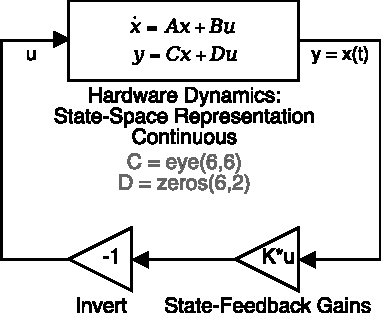
\includegraphics[trim = 0em 0em 0em 0em, clip, width=0.4\textwidth]{snap-1-0-State-Feedback-Regulator.pdf}%
\caption[{[Additional Dynamics]: State Feedback Regulator}]%
        {{[Additional Dynamics]: State Feedback Regulator%
          \label{FIG:controllerDesign:additionalDynamics:background:1p0:stateFeedbackRegulator}%
        }}%
\end{minipage}%
\end{figure}
%\vspace*{\fill}
\end{landscape}




\clearpage




\begin{landscape}
%\vspace*{\fill}
\begin{figure}[H]%
\centering%
\begin{minipage}[c][0.995\textheight][c]{0.995\linewidth}%
\centering%
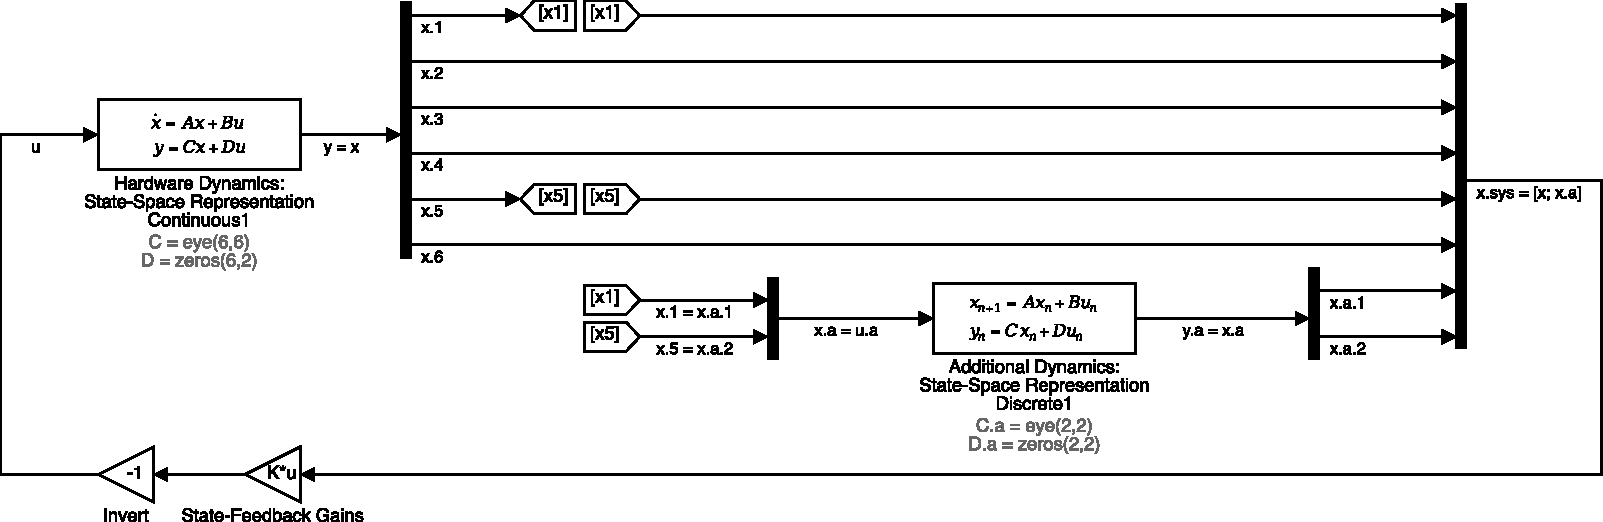
\includegraphics[trim = 0em 0em 0em 0em, clip, width=0.975\textwidth]{snap-2-0-Additional-Dynamics-(Design-View).pdf}%
\caption[{[Additional Dynamics]: 1.0 Additional Dynamics (Design View)}]%
        {{[Additional Dynamics]: 1.0 Additional Dynamics (Design View)%
          \label{FIG:controllerDesign:additionalDynamics:background:2p0:additionalDynamics:designView}%
        }}%
\end{minipage}%
\end{figure}
%\vspace*{\fill}
\end{landscape}




\clearpage




\begin{landscape}
%\vspace*{\fill}
\begin{figure}[H]%
\centering%
\begin{minipage}[c][0.995\textheight][c]{0.995\linewidth}%
\centering%
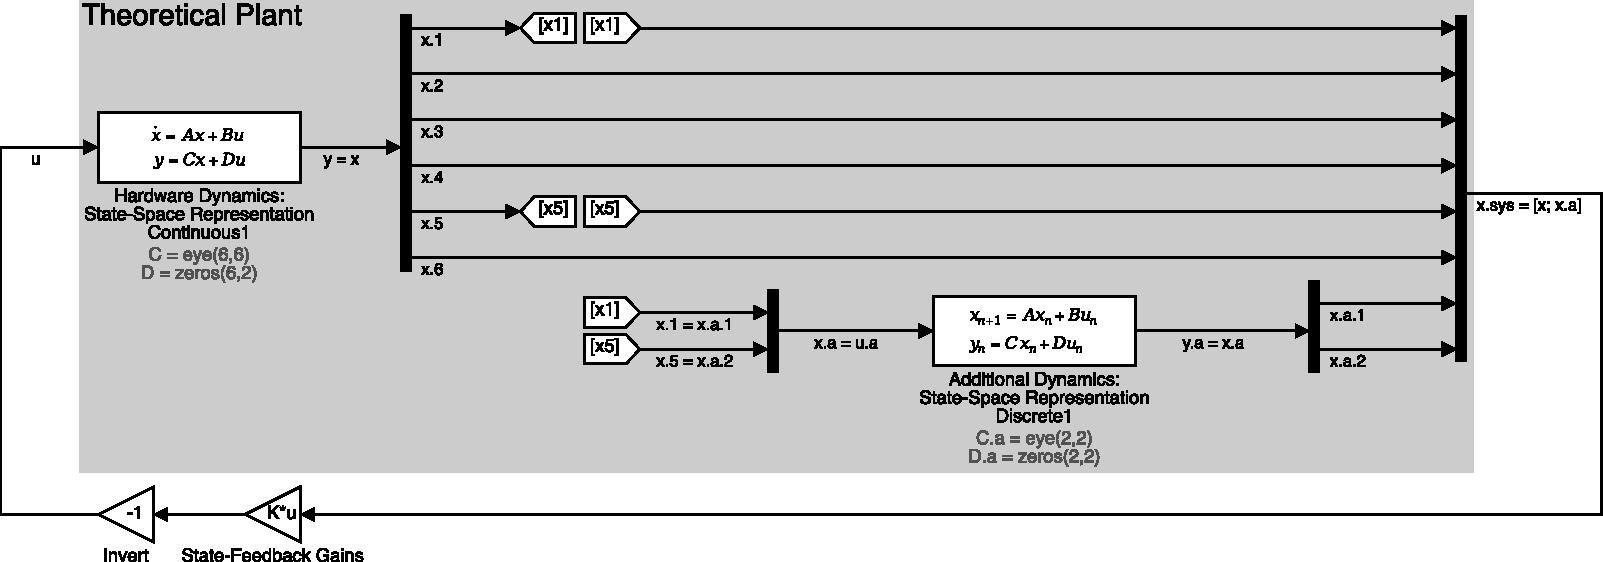
\includegraphics[trim = 0em 0em 0em 0em, clip, width=0.975\textwidth]{snap-2-1-Additional-Dynamics-(Design-View).pdf}%
\caption[{[Additional Dynamics]: 1.1 Additional Dynamics (Design View)}]%
        {{[Additional Dynamics]: 1.1 Additional Dynamics (Design View)%
          \label{FIG:controllerDesign:additionalDynamics:background:2p1:additionalDynamics:designView}%
        }}%
\end{minipage}%
\end{figure}
%\vspace*{\fill}
\end{landscape}




\clearpage




\begin{landscape}
%\vspace*{\fill}
\begin{figure}[H]%
\centering%
\begin{minipage}[c][0.995\textheight][c]{0.995\linewidth}%
\centering%
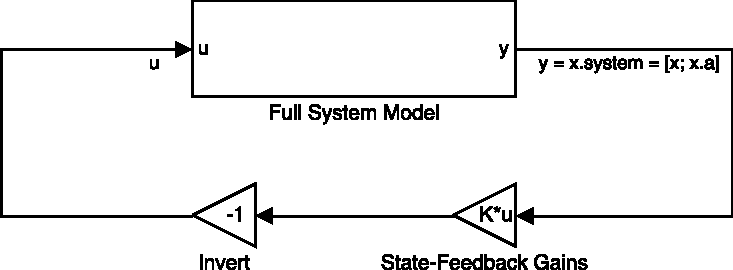
\includegraphics[trim = 0em 0em 0em 0em, clip, width=0.4\textwidth]{snap-2-2-Additional-Dynamics-(State-Feedback-Regulator-View).pdf}%
\caption[{[Additional Dynamics]: 1.2 Additional Dynamics (State Feedback Regulator View)}]%
        {{[Additional Dynamics]: 1.2 Additional Dynamics (State Feedback Regulator View)%
          \label{FIG:controllerDesign:additionalDynamics:background:2p2:additionalDynamics:stateFeedbackRegulatorView}%
        }}%
\end{minipage}%
\end{figure}
%\vspace*{\fill}
\end{landscape}




\clearpage




\begin{landscape}
%\vspace*{\fill}
\begin{figure}[H]%
\centering%
\begin{minipage}[c][0.995\textheight][c]{0.995\linewidth}%
\centering%
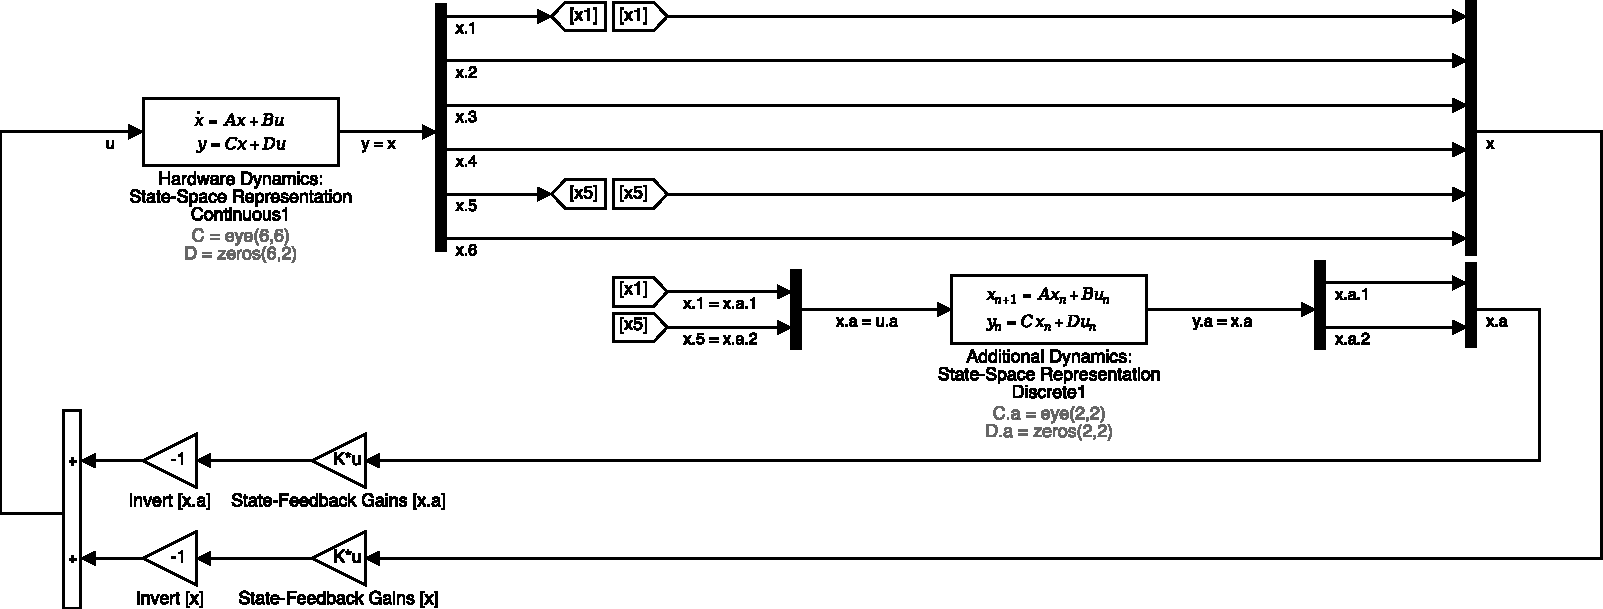
\includegraphics[trim = 0em 0em 0em 0em, clip, width=0.975\textwidth]{snap-3-0-Additional-Dynamics-(Split-Gains).pdf}%
\caption[{[Additional Dynamics]: 2.0 Additional Dynamics (Split Gains)}]%
        {{[Additional Dynamics]: 2.0 Additional Dynamics (Split Gains)%
          \label{FIG:controllerDesign:additionalDynamics:background:3p0:additionalDynamics:splitGains}%
        }}%
\end{minipage}%
\end{figure}
%\vspace*{\fill}
\end{landscape}




\clearpage




\begin{landscape}
%\vspace*{\fill}
\begin{figure}[H]%
\centering%
\begin{minipage}[c][0.995\textheight][c]{0.995\linewidth}%
\centering%
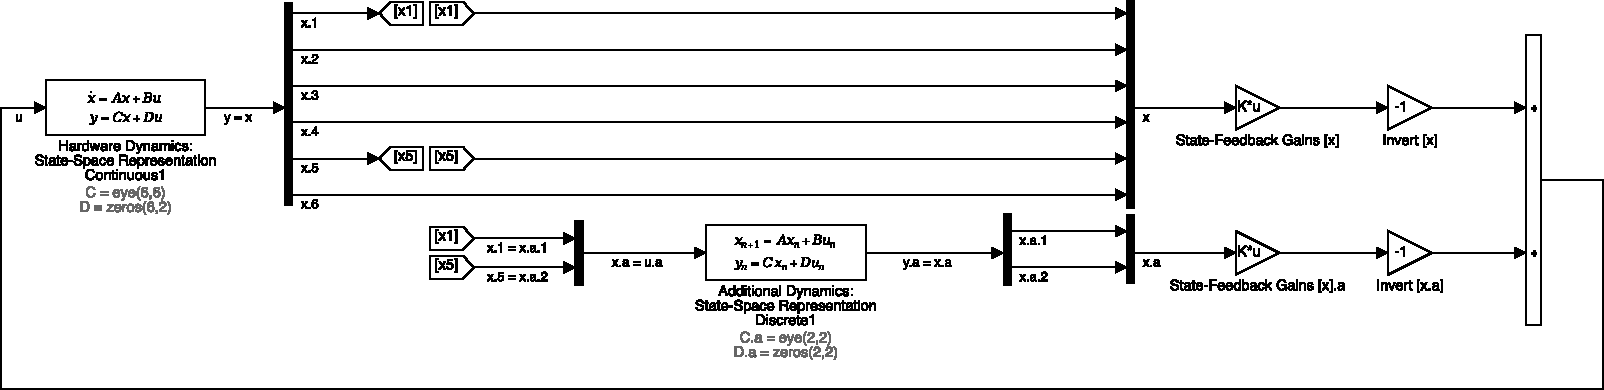
\includegraphics[trim = 0em 0em 0em 0em, clip, width=0.975\textwidth]{snap-4-0-Additional-Dynamics-(Linear-View---Plant).pdf}%
\caption[{[Additional Dynamics]: 3.0 Additional Dynamics (Linear View: Plant)}]%
        {{[Additional Dynamics]: 3.0 Additional Dynamics (Linear View: Plant)%
          \label{FIG:controllerDesign:additionalDynamics:background:4p0:additionalDynamics:linearView:plant}%
        }}%
\end{minipage}%
\end{figure}
%\vspace*{\fill}
\end{landscape}




\clearpage




\begin{landscape}
%\vspace*{\fill}
\begin{figure}[H]%
\centering%
\begin{minipage}[c][0.995\textheight][c]{0.995\linewidth}%
\centering%
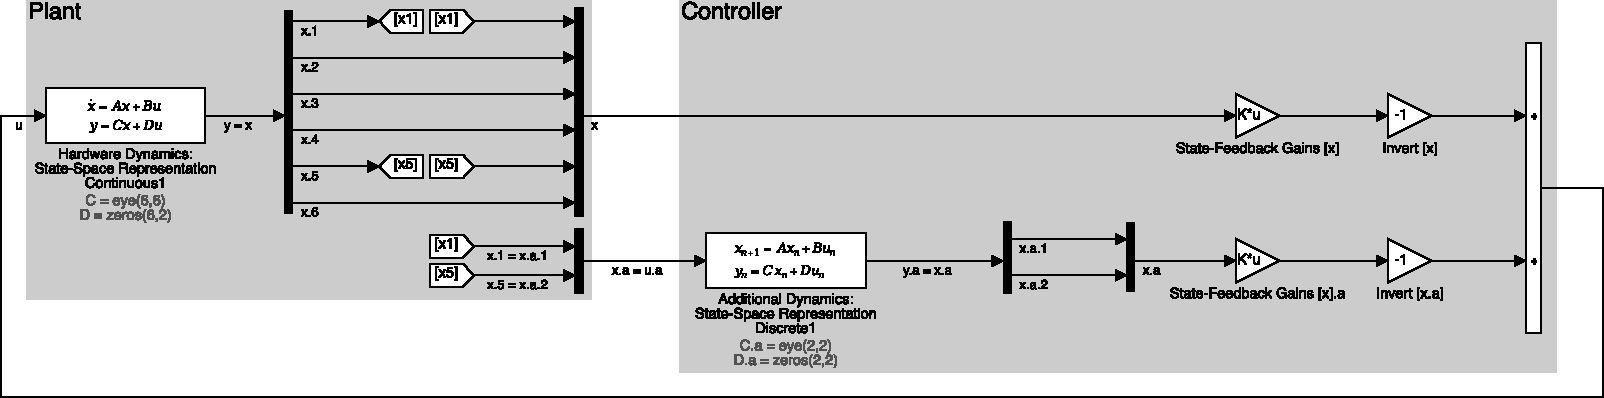
\includegraphics[trim = 0em 0em 0em 0em, clip, width=0.975\textwidth]{snap-4-1-Additional-Dynamics-(Linear-View---Plant).pdf}%
\caption[{[Additional Dynamics]: 3.1 Additional Dynamics (Linear View: Plant)}]%
        {{[Additional Dynamics]: 3.1 Additional Dynamics (Linear View: Plant)%
          \label{FIG:controllerDesign:additionalDynamics:background:4p1:additionalDynamics:linearView:plant}%
        }}%
\end{minipage}%
\end{figure}
%\vspace*{\fill}
\end{landscape}




\clearpage




\begin{landscape}
%\vspace*{\fill}
\begin{figure}[H]%
\centering%
\begin{minipage}[c][0.995\textheight][c]{0.995\linewidth}%
\centering%
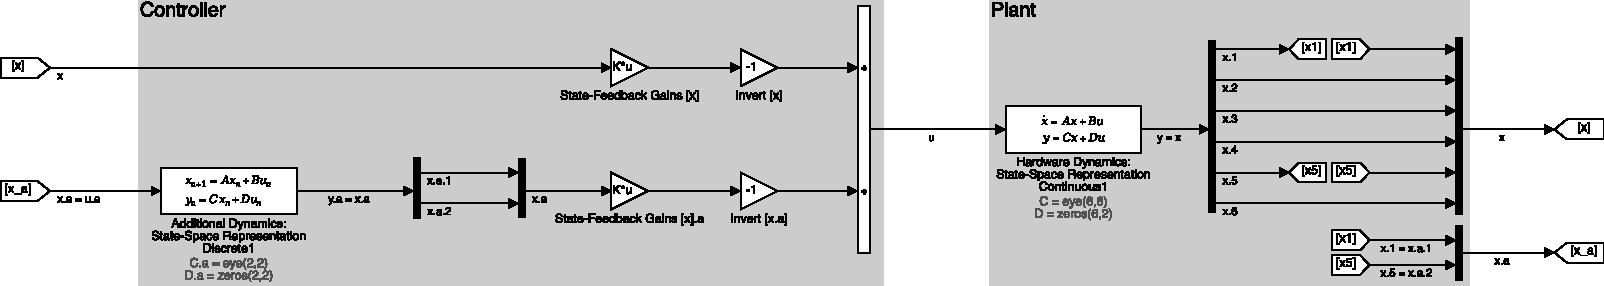
\includegraphics[trim = 0em 0em 0em 0em, clip, width=0.975\textwidth]{snap-5-0-Additional-Dynamics-(Linear-View---Controller)}%
\caption[{[Additional Dynamics]: 4.0 Additional Dynamics (Linear View: Controller)}]%
        {{[Additional Dynamics]: 4.0 Additional Dynamics (Linear View: Controller)%
          \label{FIG:controllerDesign:additionalDynamics:background:5p0:additionalDynamics:linearView:controller}%
        }}%
\end{minipage}%
\end{figure}
%\vspace*{\fill}
\end{landscape}




\clearpage




\begin{landscape}
%\vspace*{\fill}
\begin{figure}[H]%
\centering%
\begin{minipage}[c][0.995\textheight][c]{0.995\linewidth}%
\centering%
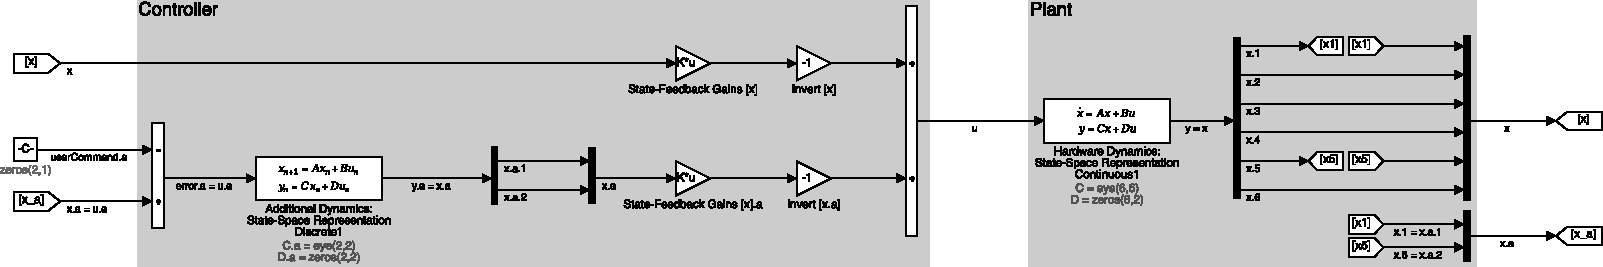
\includegraphics[trim = 0em 0em 0em 0em, clip, width=0.975\textwidth]{snap-6-0-Additional-Dynamics-(Linear-View---User).pdf}%
\caption[{[Additional Dynamics]: 4.0 Additional Dynamics with Reference Signal (Linear View: User)}]%
        {{[Additional Dynamics]: 4.0 Additional Dynamics with Reference Signal (Linear View: User)%
          \label{FIG:controllerDesign:additionalDynamics:background:6p0:additionalDynamics:linearView:user}%
        }}%
\end{minipage}%
\end{figure}
%\vspace*{\fill}
\end{landscape}




\clearpage




\begin{landscape}
%\vspace*{\fill}
\begin{figure}[H]%
\centering%
\begin{minipage}[c][0.995\textheight][c]{0.995\linewidth}%
\centering%
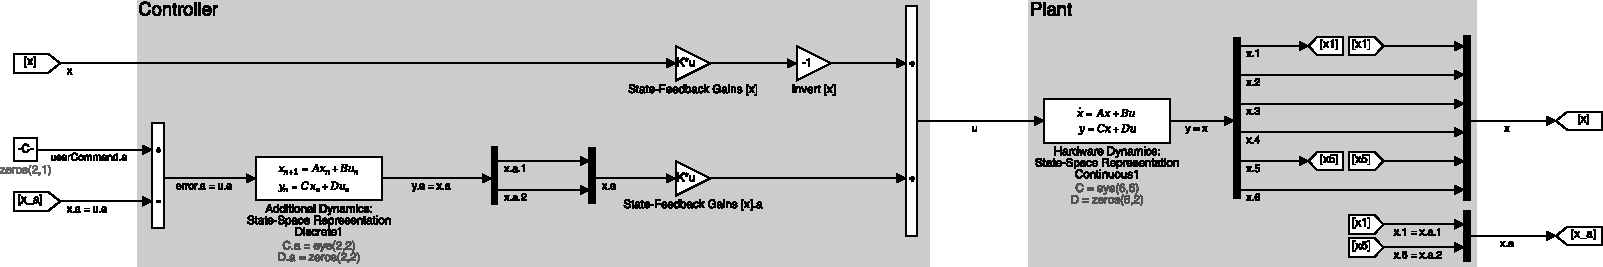
\includegraphics[trim = 0em 0em 0em 0em, clip, width=0.975\textwidth]{snap-6-1-Additional-Dynamics-(Linear-View---User).pdf}%
\caption[{[Additional Dynamics]: 4.0 Additional Dynamics with Reference Signal (Linear View: User)}]%
        {{[Additional Dynamics]: 4.0 Additional Dynamics with Reference Signal (Linear View: User)%
          \label{FIG:controllerDesign:additionalDynamics:background:6p1:additionalDynamics:linearView:user}%
        }}%
\end{minipage}%
\end{figure}
%\vspace*{\fill}
\end{landscape}




\clearpage




\subsubsection{Reference Signal}
\label{SEC:controllerDesign:additionalDynamics:background:referenceSignal}


Recall that a standard state-feedback regulator 
simply brings its inputs, 
{\fns[\tif{in this case, system states $x$ and $x_{a}$}]},
to zero.
If it is desired that a controller input be brought to a value other than zero,
a reference signal may be implemented.

In these cases, 
rather than input the controller with a state which the controller will bring to zero,
the controller is input with 
the difference between the state value and the reference {\fns[\tif{desired}]} value.
This difference is commonly known as the error signal.
Once the error signal is brought to zero for a given state,
the state will be equivalent to the desired reference value.

Returning to system depiction,
a reference command is implemented,
as depicted in Figure~%
\ref{FIG:controllerDesign:additionalDynamics:background:6p0:additionalDynamics:linearView:user}.

Note that the reference signal receives the negative.
Inverting the system state alters the system equation,
and could cause the system to become unstable.

Despite this fact, it is sometimes more common to see 
the system state subtracted from the reference signal.
To correctly achieve this,
once the reference signal is implemented,
either side of the difference equation is multiplied by -1.
The negative on the input side is distributed to both inputs.
The output of the difference equation is the input of the additional dynamics;
thus, when the negative appears on the output side of the difference equation,
a negative exists on either side of the additional dynamics equation.

Recall that all state-space representations are linear;
therefore, the input and the output may be multiplied by the same value.
In this case, the negative may be divided out on both sides.

These changes are depicted in Figure~%
\ref{FIG:controllerDesign:additionalDynamics:background:6p1:additionalDynamics:linearView:user}.




\clearpage




\end{document}











% !TEX TS-program = arara
%  arara: lmkclean
%  arara: pdflatex: {   draft: yes, options: '-file-line-error -halt-on-error' }
%  arara: biber
%  arara: pdflatex: {   draft: yes, options: '-file-line-error -halt-on-error' }
%  arara: pdflatex: { synctex: yes, options: '-file-line-error -halt-on-error' }
%  arara: lmkclean
\documentclass[crop=false,float=true,class=scrreprt]{standalone}

\providecommand{\main}{../../../..}
\input{\main/Subfiles/0-Preamble/0-Preamble.tex}  % Preamble [document configuration]

\begin{document}

\subsection{Tracking System}
\label{SEC:controllerDesign:additionalDynamics:trackingSystem}

Additional dynamics may be incorporated to improve reference tracking.
When implemented for this purpose, the additional dynamics are known as a tracking system.

In the case of a tracking system, 
an \tif{integrator} may be implemented as the additional dynamics
to track a constant reference exactly, or 
to track a slowly varying reference approximately.

Integrators are also able to mitigate constant disturbances.
Incidentally, the MinSeg M2V3 system uses gyroscopes as body angular velocity $\psi$ sensors.
Bias is inherent in the output of a gyroscope;
therefore, the use of such an integrator as a tracking system has an additional benefit:
it will mitigate the effects of bias from a gyroscope output, 
whether directly or within terms which are derivative of the gyroscope output.

Thus, in the case of the two-wheeled robot, 
integrators are implemented as additional dynamics for the states representing 
wheel angular position $\theta$ and body angular position (yaw) $\phi_{y}$.
This establishes a tracking system, {\fns[\tif{an augmented method of state feedback regulation}]}, for the system.
The state-space representation of the integrator is exhibited in Equation~%
\eqref{EQN:controllerDesign:additionalDynamics:trackingSystem:integrator:analog}.

\vspace{-0em}

\begin{equation}
\label{EQN:controllerDesign:additionalDynamics:trackingSystem:integrator:analog}
\begin{array}{ccccccccc}
\uns{\mbf{\dot{x}}(t)}{n x 1}
& = &
\begin{bmatrix}
0 & 0 \\
0 & 0 \\
\end{bmatrix}
& \cdot &
\uns{\mbf{x}(t)}{n x 1} 
& + & 
\begin{bmatrix}
1 & 0 \\
0 & 1 \\
\end{bmatrix}
& \cdot &
\begin{bmatrix}
e_{\theta_{\hphantom{y}}} (t) \\
e_{\phi_{y}}              (t) \\
\end{bmatrix}
\\[+2em]
\uns{\mbf{y}(t)}{m x 1}
& = &
\begin{bmatrix}
1 & 0 \\
0 & 1 \\
\end{bmatrix}
& \cdot &
\uns{\mbf{x}(t)}{n x 1}
& + &
\begin{bmatrix}
0 & 0 \\
0 & 0 \\
\end{bmatrix}
& \cdot &
\begin{bmatrix}
e_{\theta_{\hphantom{y}}} (t) \\
e_{\phi_{y}}              (t) \\
\end{bmatrix}
\end{array}
\end{equation}




\clearpage




\subsubsection{Discrete Additional Dynamics}


Since the additional dynamics will be processed on a microcontroller,
the additional dynamics will be digital;
thus, a continuous-to-discrete conversion will be necessary.
A digital integrator is an established case which is exhibited in Equation~%
\eqref{EQN:controllerDesign:additionalDynamics:trackingSystem:integrator:discrete}.

\vspace{-0em}

\begin{equation}
\label{EQN:controllerDesign:additionalDynamics:trackingSystem:integrator:discrete}
\begin{array}{ccccccccc}
\uns{\mbf{\dot{x}}[k+1]}{n x 1}
& = &
\begin{bmatrix}
1 & 0 \\
0 & 1 \\
\end{bmatrix}
& \cdot &
\uns{\mbf{x}[k]}{n x 1}
& + & 
\begin{bmatrix}
1 & 0 \\
0 & 1 \\
\end{bmatrix}
& \cdot &
\begin{bmatrix}
e_{\theta_{\hphantom{y}}} [k] \\
e_{\phi_{y}}              [k] \\
\end{bmatrix}
\\[+2em]
\uns{\mbf{y}[k]}{m x 1}
& = &
\begin{bmatrix}
1 & 0 \\
0 & 1 \\
\end{bmatrix}
& \cdot &
\uns{\mbf{x}[k]}{n x 1}
& + &
\begin{bmatrix}
0 & 0 \\
0 & 0 \\
\end{bmatrix}
& \cdot &
\begin{bmatrix}
e_{\theta_{\hphantom{y}}} [k] \\
e_{\phi_{y}}              [k] \\
\end{bmatrix}
\end{array}
\end{equation}




\clearpage




\end{document}











% !TEX TS-program = arara
%  arara: lmkclean
%  arara: pdflatex: {   draft: yes, options: '-file-line-error -halt-on-error' }
%  arara: biber
%  arara: pdflatex: {   draft: yes, options: '-file-line-error -halt-on-error' }
%  arara: pdflatex: { synctex: yes, options: '-file-line-error -halt-on-error' }
%  arara: lmkclean
\documentclass[crop=false,float=true,class=scrreprt]{standalone}

\providecommand{\main}{../../../..}
\input{\main/Subfiles/0-Preamble/0-Preamble.tex}  % Preamble [document configuration]

\begin{document}

\subsection{Control Gains}
\label{SEC:controllerDesign:additionalDynamics}

Once the additional dynamics are established,
state feedback gains must be calculated.
Multiple methods exist to calculate these gains.
The most established methods involve optimization or pole-placement.


\subsubsection{Optimal}
\label{SEC:controllerDesign:additionalDynamics:optimal}

Several optimal control techniques exist
\cite{REF:textbook:1995-lewis}.
This section will focus on linear quadratic regulation techniques.

%\subsubsubsection{Background}
\subsubsubsection{Implementation}

In order to determine the feedback gains of the system,
the state-space representation of the system,
{\fns[\tif{the plant and the additional dynamics}]},
is input into a 
discrete linear quadratic regulator gain-calculation Matlab function, \tif{dlqr},
which outputs state-feedback gains which best minimize the quadratic cost function.
The Matlab function also requires quadratic cost function matrices $Q$ and $R$ as inputs.

The quadratic cost matrices $Q$ and $R$ were determined through trial and error;
however, some constraints existed.
The $Q$ and $R$ matrices were both diagonal matrices;
{\fns[\tif{thus, all indices which are not on the diagonal are equal to zero}]}.
Also, the $R$ matrix was left as an identity matrix until the $Q$ matrix 
established desirable behavior.
Once desirable behavior was established, 
the option of multiplying the $R$ matrix by a scalar value {\fns[\tif{greater than one}]} became a consideration.

Multiplying the $R$ matrix by a scalar value decreases the response time of the controller;
however, this also decreases the peak magnitude of the control output,
{\fns[\tif{in this case, motor voltage}]}.
While a decreased response time is generally undesirable,
the reduction of the control output can be necessary in certain circumstances.
For example, the maximum permissible value for the control output, motor voltage, 
is limited by the nominal voltage provided by the hardware power source.




\clearpage




\subsubsubsection{Results: Simulation}
\label{SEC:controllerDesign:additionalDynamics:optimal:results:simulation}

To demonstrate the capabilities of the device,
a dynamic command is provided which attempts to move the device
in the shape of an eight $8$ on the ground
while maintaining balance.

The specific Q and R weighting matrices which were selected to calculate the control gains
are exhibited in Equation~%
\eqref{EQN:controllerDesign:additionalDynamics:optimal:results:simulation:QR}.

\vspace{-0em}
\begin{equation}
\label{EQN:controllerDesign:additionalDynamics:optimal:results:simulation:QR}
\begin{array}{ccccl}
Q
& = &
\displaystyle\uns{\mrm{I}}{6 x 6}
& \cdot &
\begin{bmatrix}
6 & 1 & 1 & 1 & 1 & 1 & 21 & 11
\end{bmatrix}^{\mrm{T}}
\\[+1em]
R
& = &
\displaystyle\uns{\mrm{I}}{2 x 2}
& \cdot &
\begin{bmatrix}
1 & 1
\end{bmatrix}^{\mrm{T}}
\end{array}
\end{equation}
\vspace{-0.5em}

Recall that Q is with respect to the states of the global system,
{\fns[\tif{plant and reference tracking dynamics}]}
and 
that R is with respect to inputs of the global system
{\fns[\tif{reference tracking input error}]}.

Note that the greatest weights have been applied to the reference tracking states,
and also that additional weight has been provided to the wheel angular position state $\theta$,
in the cases of the plant states as well as the reference tracking states, respectively.

This results in the feedback gain matrices $K$ exhibited in Equation~%
\eqref{EQN:controllerDesign:additionalDynamics:optimal:results:simulation:K}.


Additionally, the device starts at a body angular position (pitch) $\phi_x$ of $0.03\ [rad]$.
This represents the inability to start the device at a perfect angle.
This causes additional transients in the initial milliseconds of operation.

Figures
\ref{FIG:controllerDesign:additionalDynamics:optimal:results:simulation:theta}~%
-~%
\ref{FIG:controllerDesign:additionalDynamics:optimal:results:simulation:vMotorDriver}
depict the system state during its operation
while completing its response to a figure-eight linear position command.




\clearpage




\begin{landscape}

\vspace*{\fill}
\begin{equation}
\fns
\label{EQN:controllerDesign:additionalDynamics:optimal:results:simulation:K}
\begin{array}{ccl}
K_{plant}
& = &
\begin{bmatrix}
-50.3100392458413 & -67.5072785023266 & -6.36629920161377 & -1.55714590289198 & -31.3872481064794 & -0.0172137559799668 \\
-50.3100392458415 & -67.5072785023269 & -6.36629920161380 & -1.55714590289199 & +31.3872481064798 & +0.0172137559799669 \\
\end{bmatrix}^{\mrm{T}}
\\[+4em]
K_{referenceTracking}
& = &
\begin{bmatrix}
-2.29913264446660 & -2.07850353527147 \\
-2.29913264446662 & +2.07850353527155 \\
\end{bmatrix}^{\mrm{T}}
\end{array}
\end{equation}
\vspace*{+4.5em}
\vspace*{\fill}

\end{landscape}




\clearpage




\vspace*{\fill}
\begin{figure}[H]%
\centering%
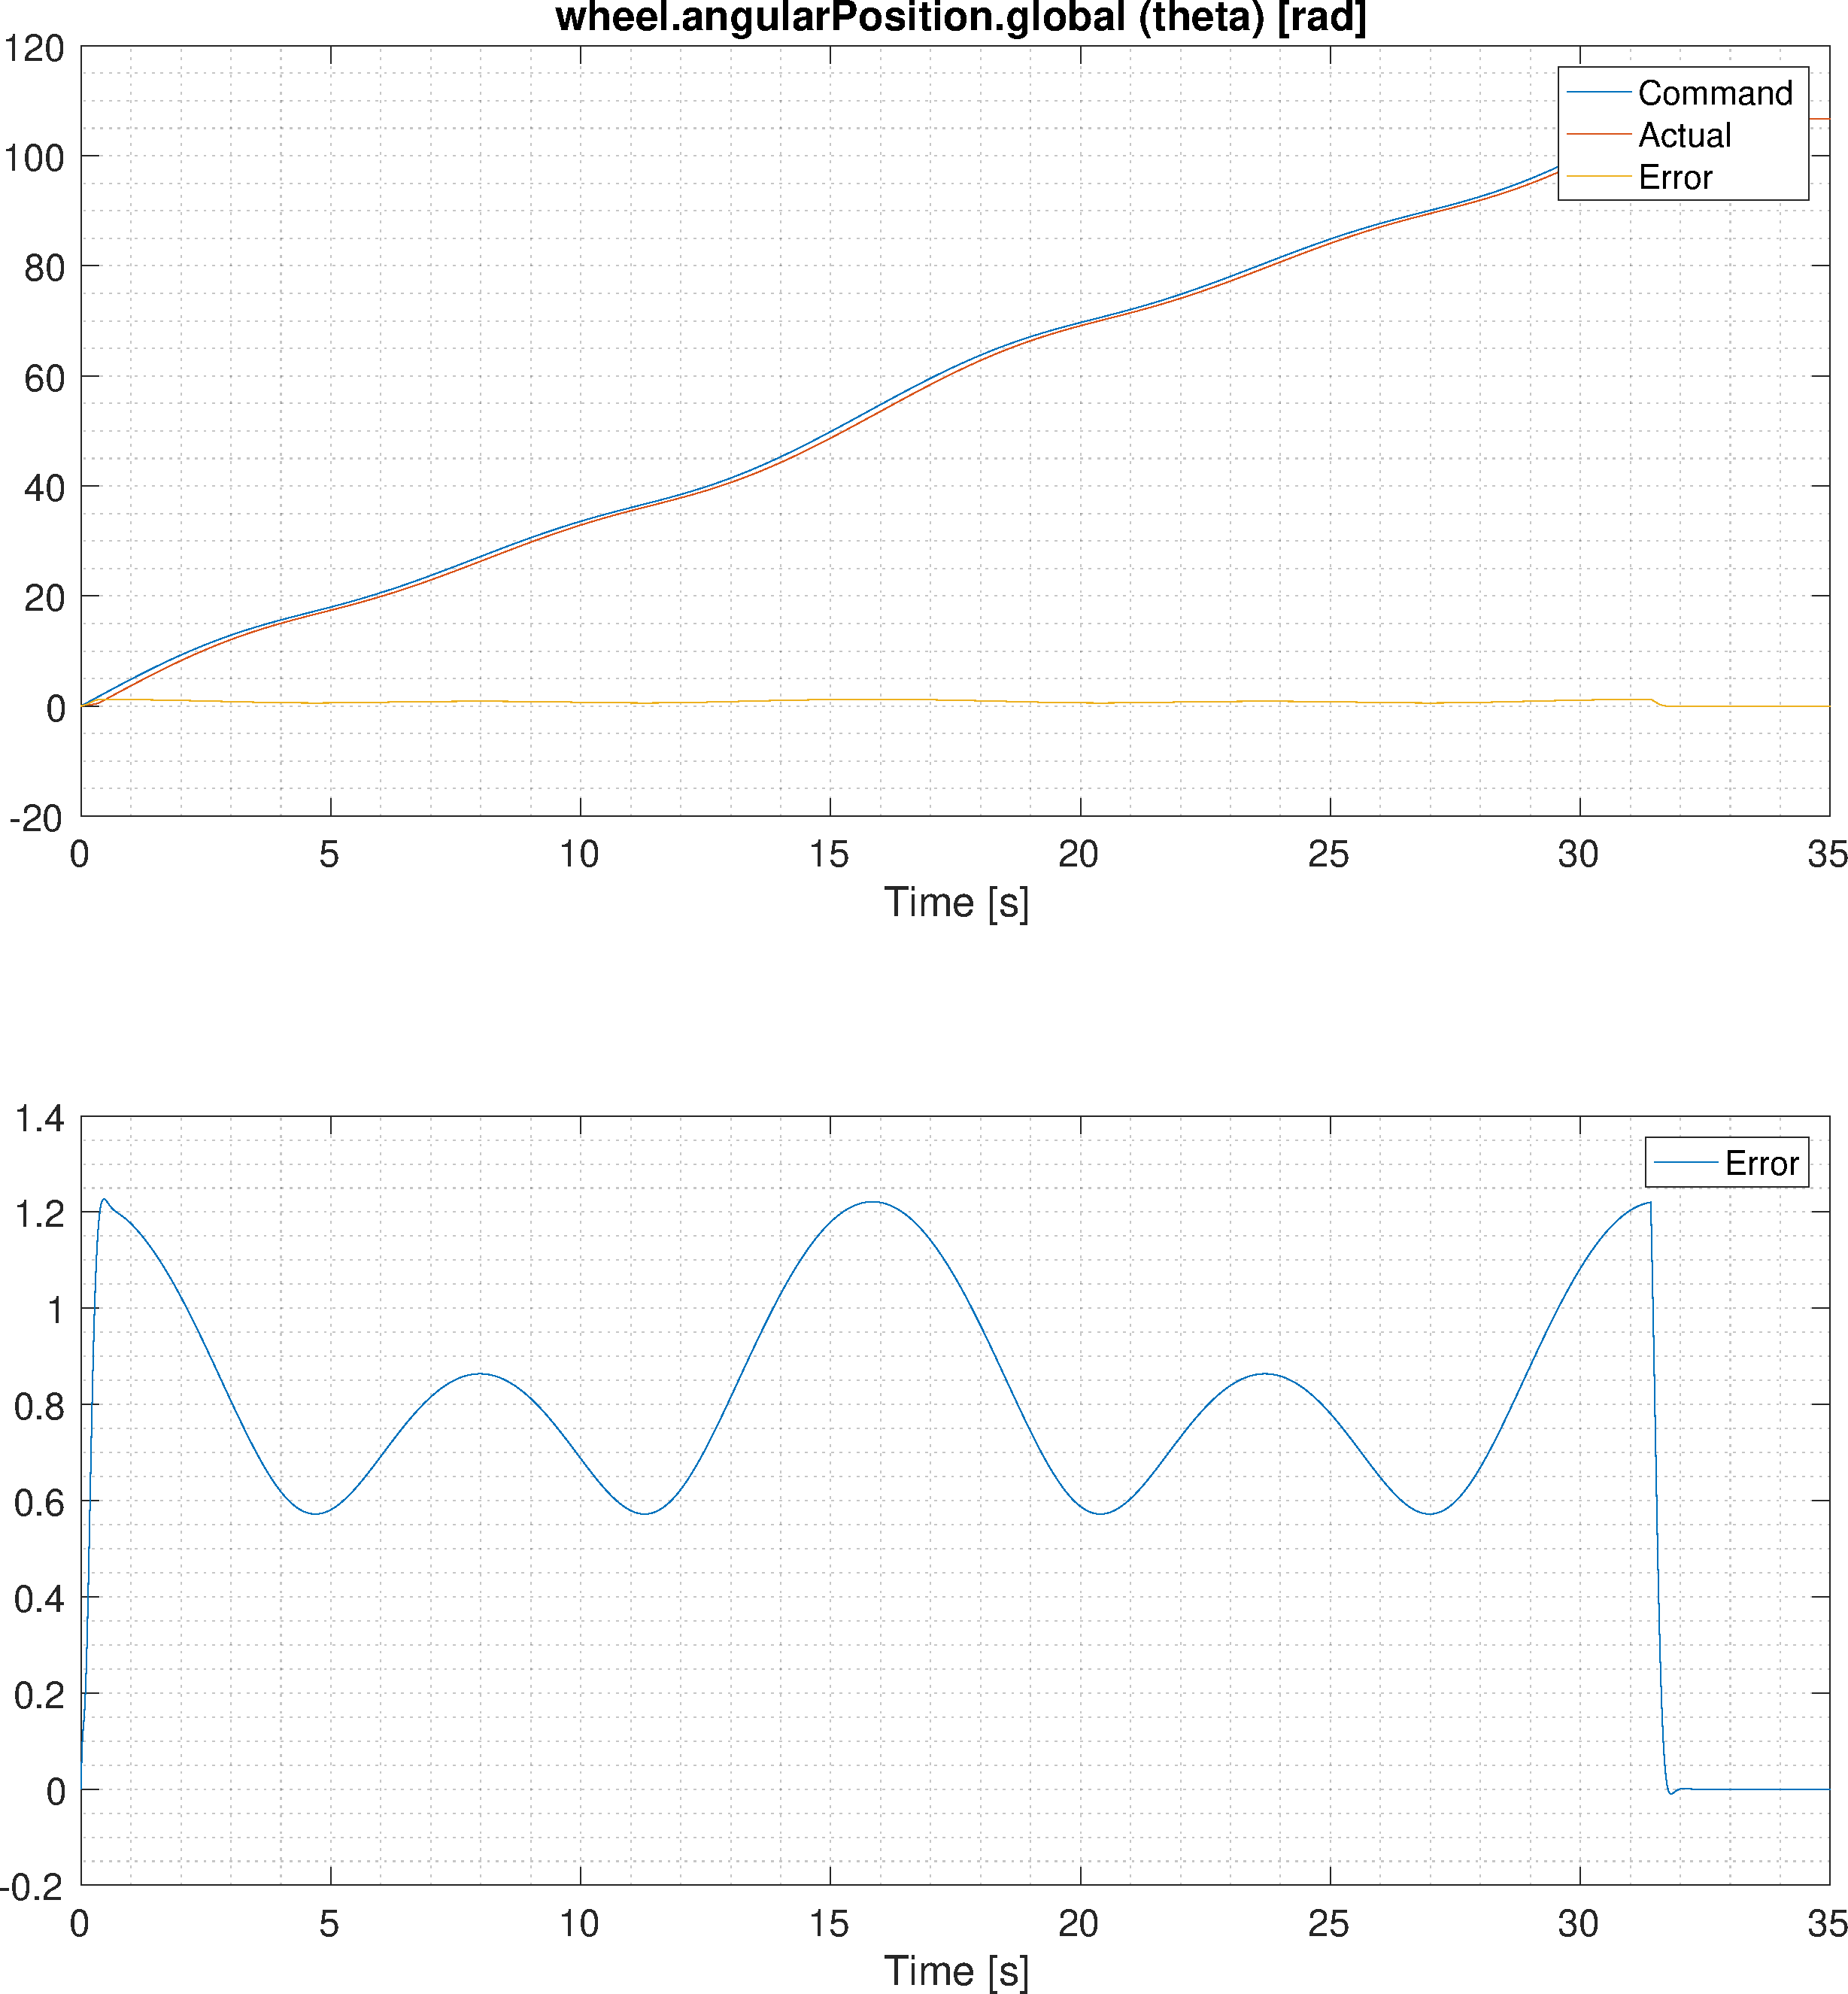
\includegraphics[trim = 0em 0em 0em 0em, clip, width=0.975\textwidth]{theta.pdf}%
\caption[{[Control Gains: LQR]: Simulation Results: Wheel Angular Position $\theta$}]%
        {{[Control Gains: LQR]: Simulation Results: Wheel Angular Position $\theta$%
          \label{FIG:controllerDesign:additionalDynamics:optimal:results:simulation:theta}%
        }}%
\end{figure}
\vspace*{\fill}




\clearpage





\vspace*{\fill}
\begin{figure}[H]%
\centering%
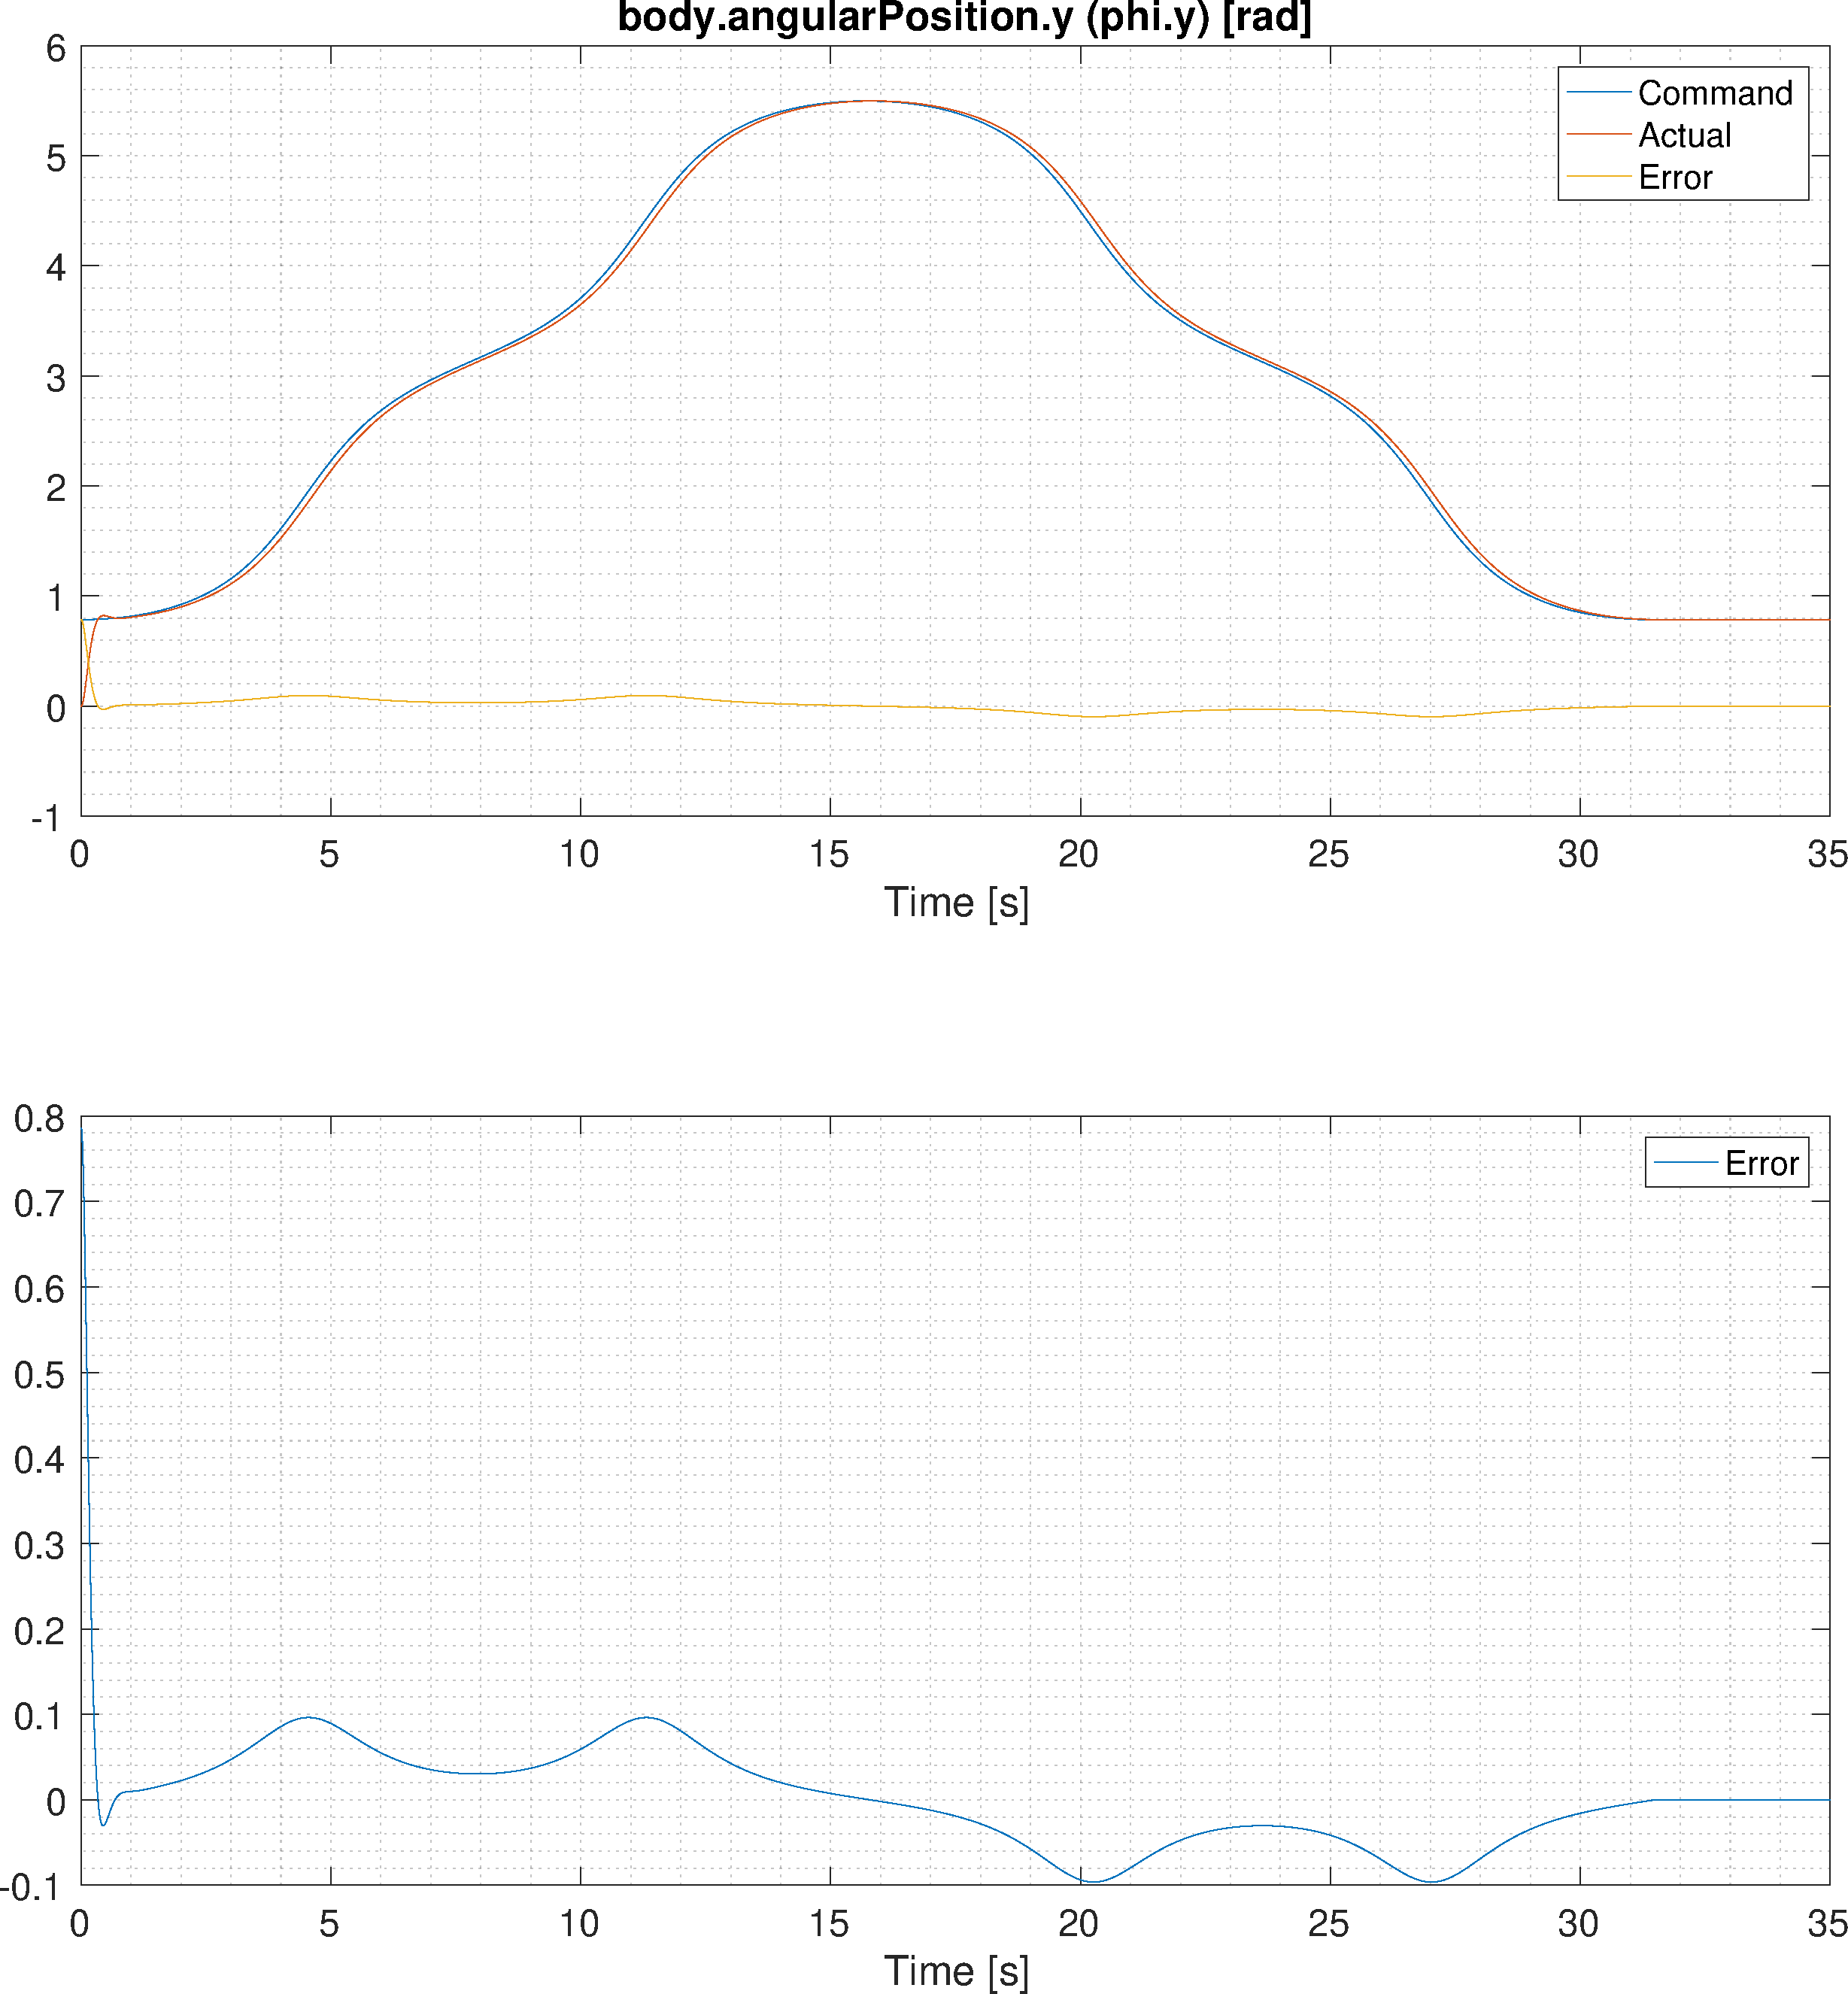
\includegraphics[trim = 0em 0em 0em 0em, clip, width=0.975\textwidth]{phi-y.pdf}%
\caption[{[Control Gains: LQR]: Simulation Results: Body Angular Position $\phi_{y}$}]%
        {{[Control Gains: LQR]: Simulation Results: Body Angular Position $\phi_{y}$%
          \label{FIG:controllerDesign:additionalDynamics:optimal:results:simulation:phiY}%
        }}%
\end{figure}
\vspace*{\fill}




\clearpage





\vspace*{\fill}
\begin{figure}[H]%
\centering%
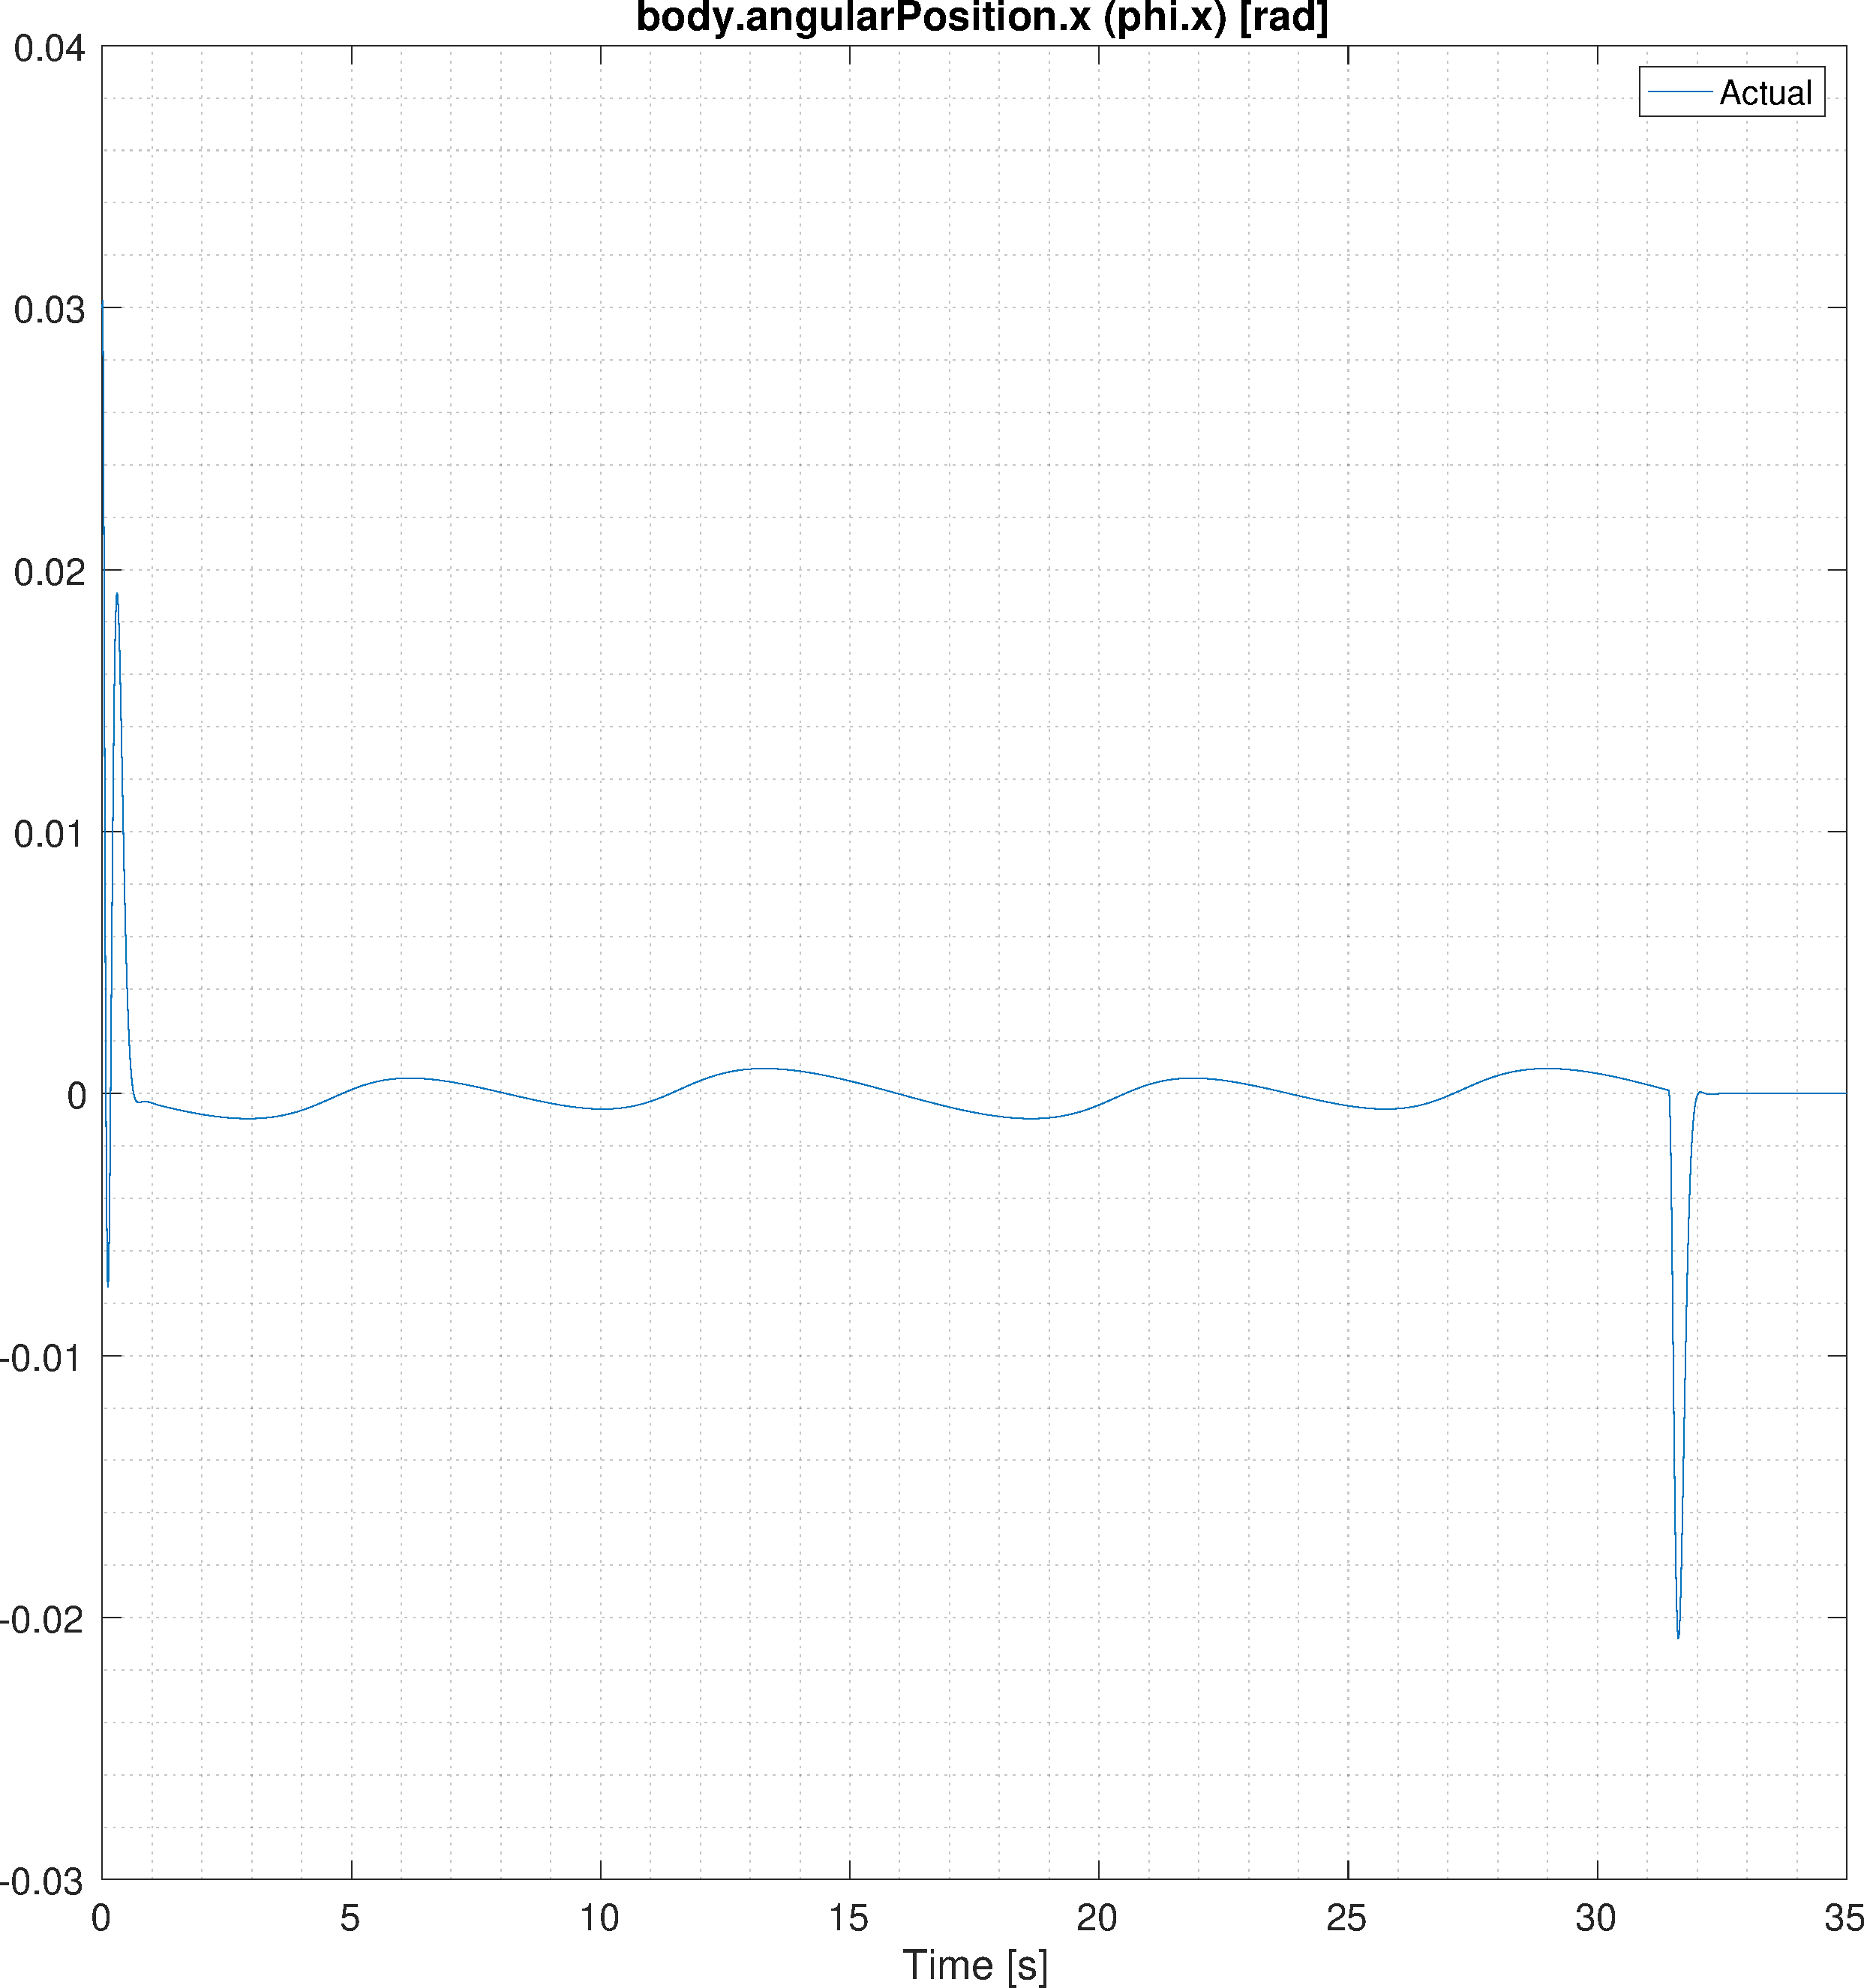
\includegraphics[trim = 0em 0em 0em 0em, clip, width=0.975\textwidth]{phi-x.pdf}%
\caption[{[Control Gains: LQR]: Simulation Results: Body Angular Position $\phi_{x}$}]%
        {{[Control Gains: LQR]: Simulation Results: Body Angular Position $\phi_{x}$%
          \label{FIG:controllerDesign:additionalDynamics:optimal:results:simulation:phiX}%
        }}%
\end{figure}
\vspace*{\fill}




\clearpage





\vspace*{\fill}
\begin{figure}[H]%
\centering%
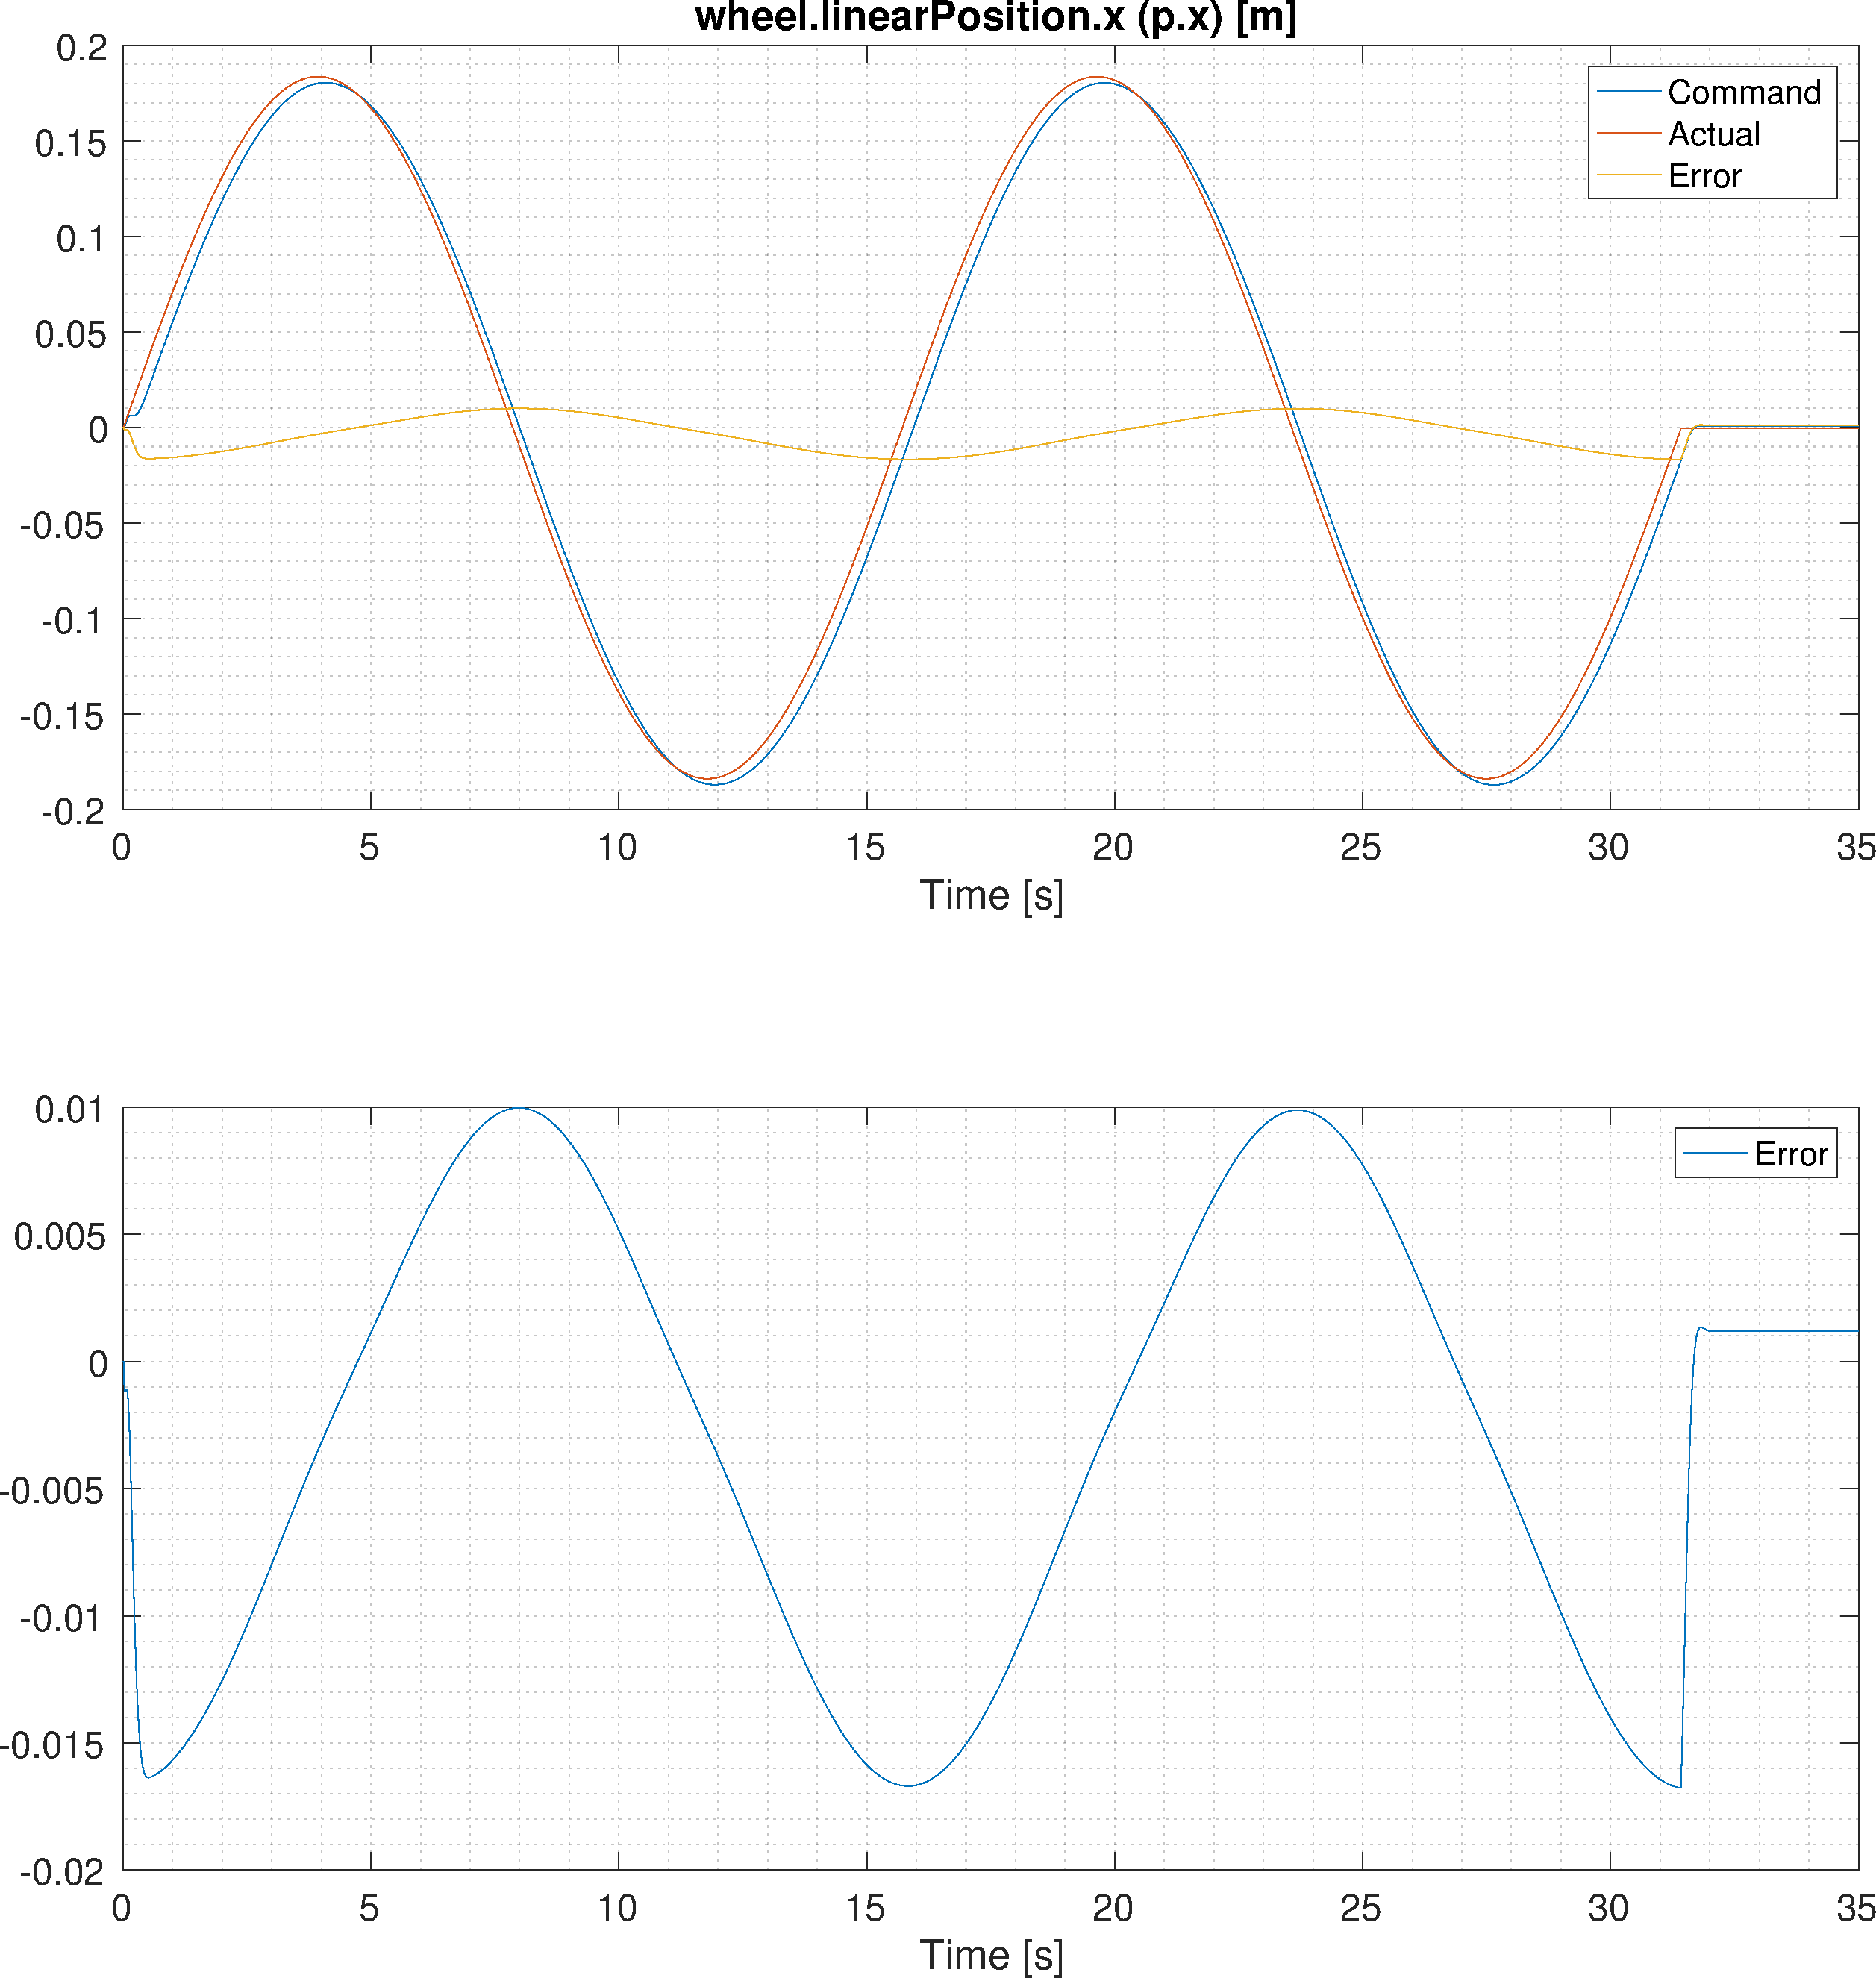
\includegraphics[trim = 0em 0em 0em 0em, clip, width=0.975\textwidth]{p-x.pdf}%
\caption[{[Control Gains: LQR]: Simulation Results: Wheel Linear Position $p_{x}$}]%
        {{[Control Gains: LQR]: Simulation Results: Wheel Linear Position $p_{x}$%
          \label{FIG:controllerDesign:additionalDynamics:optimal:results:simulation:pX}%
        }}%
\end{figure}
\vspace*{\fill}




\clearpage





\vspace*{\fill}
\begin{figure}[H]%
\centering%
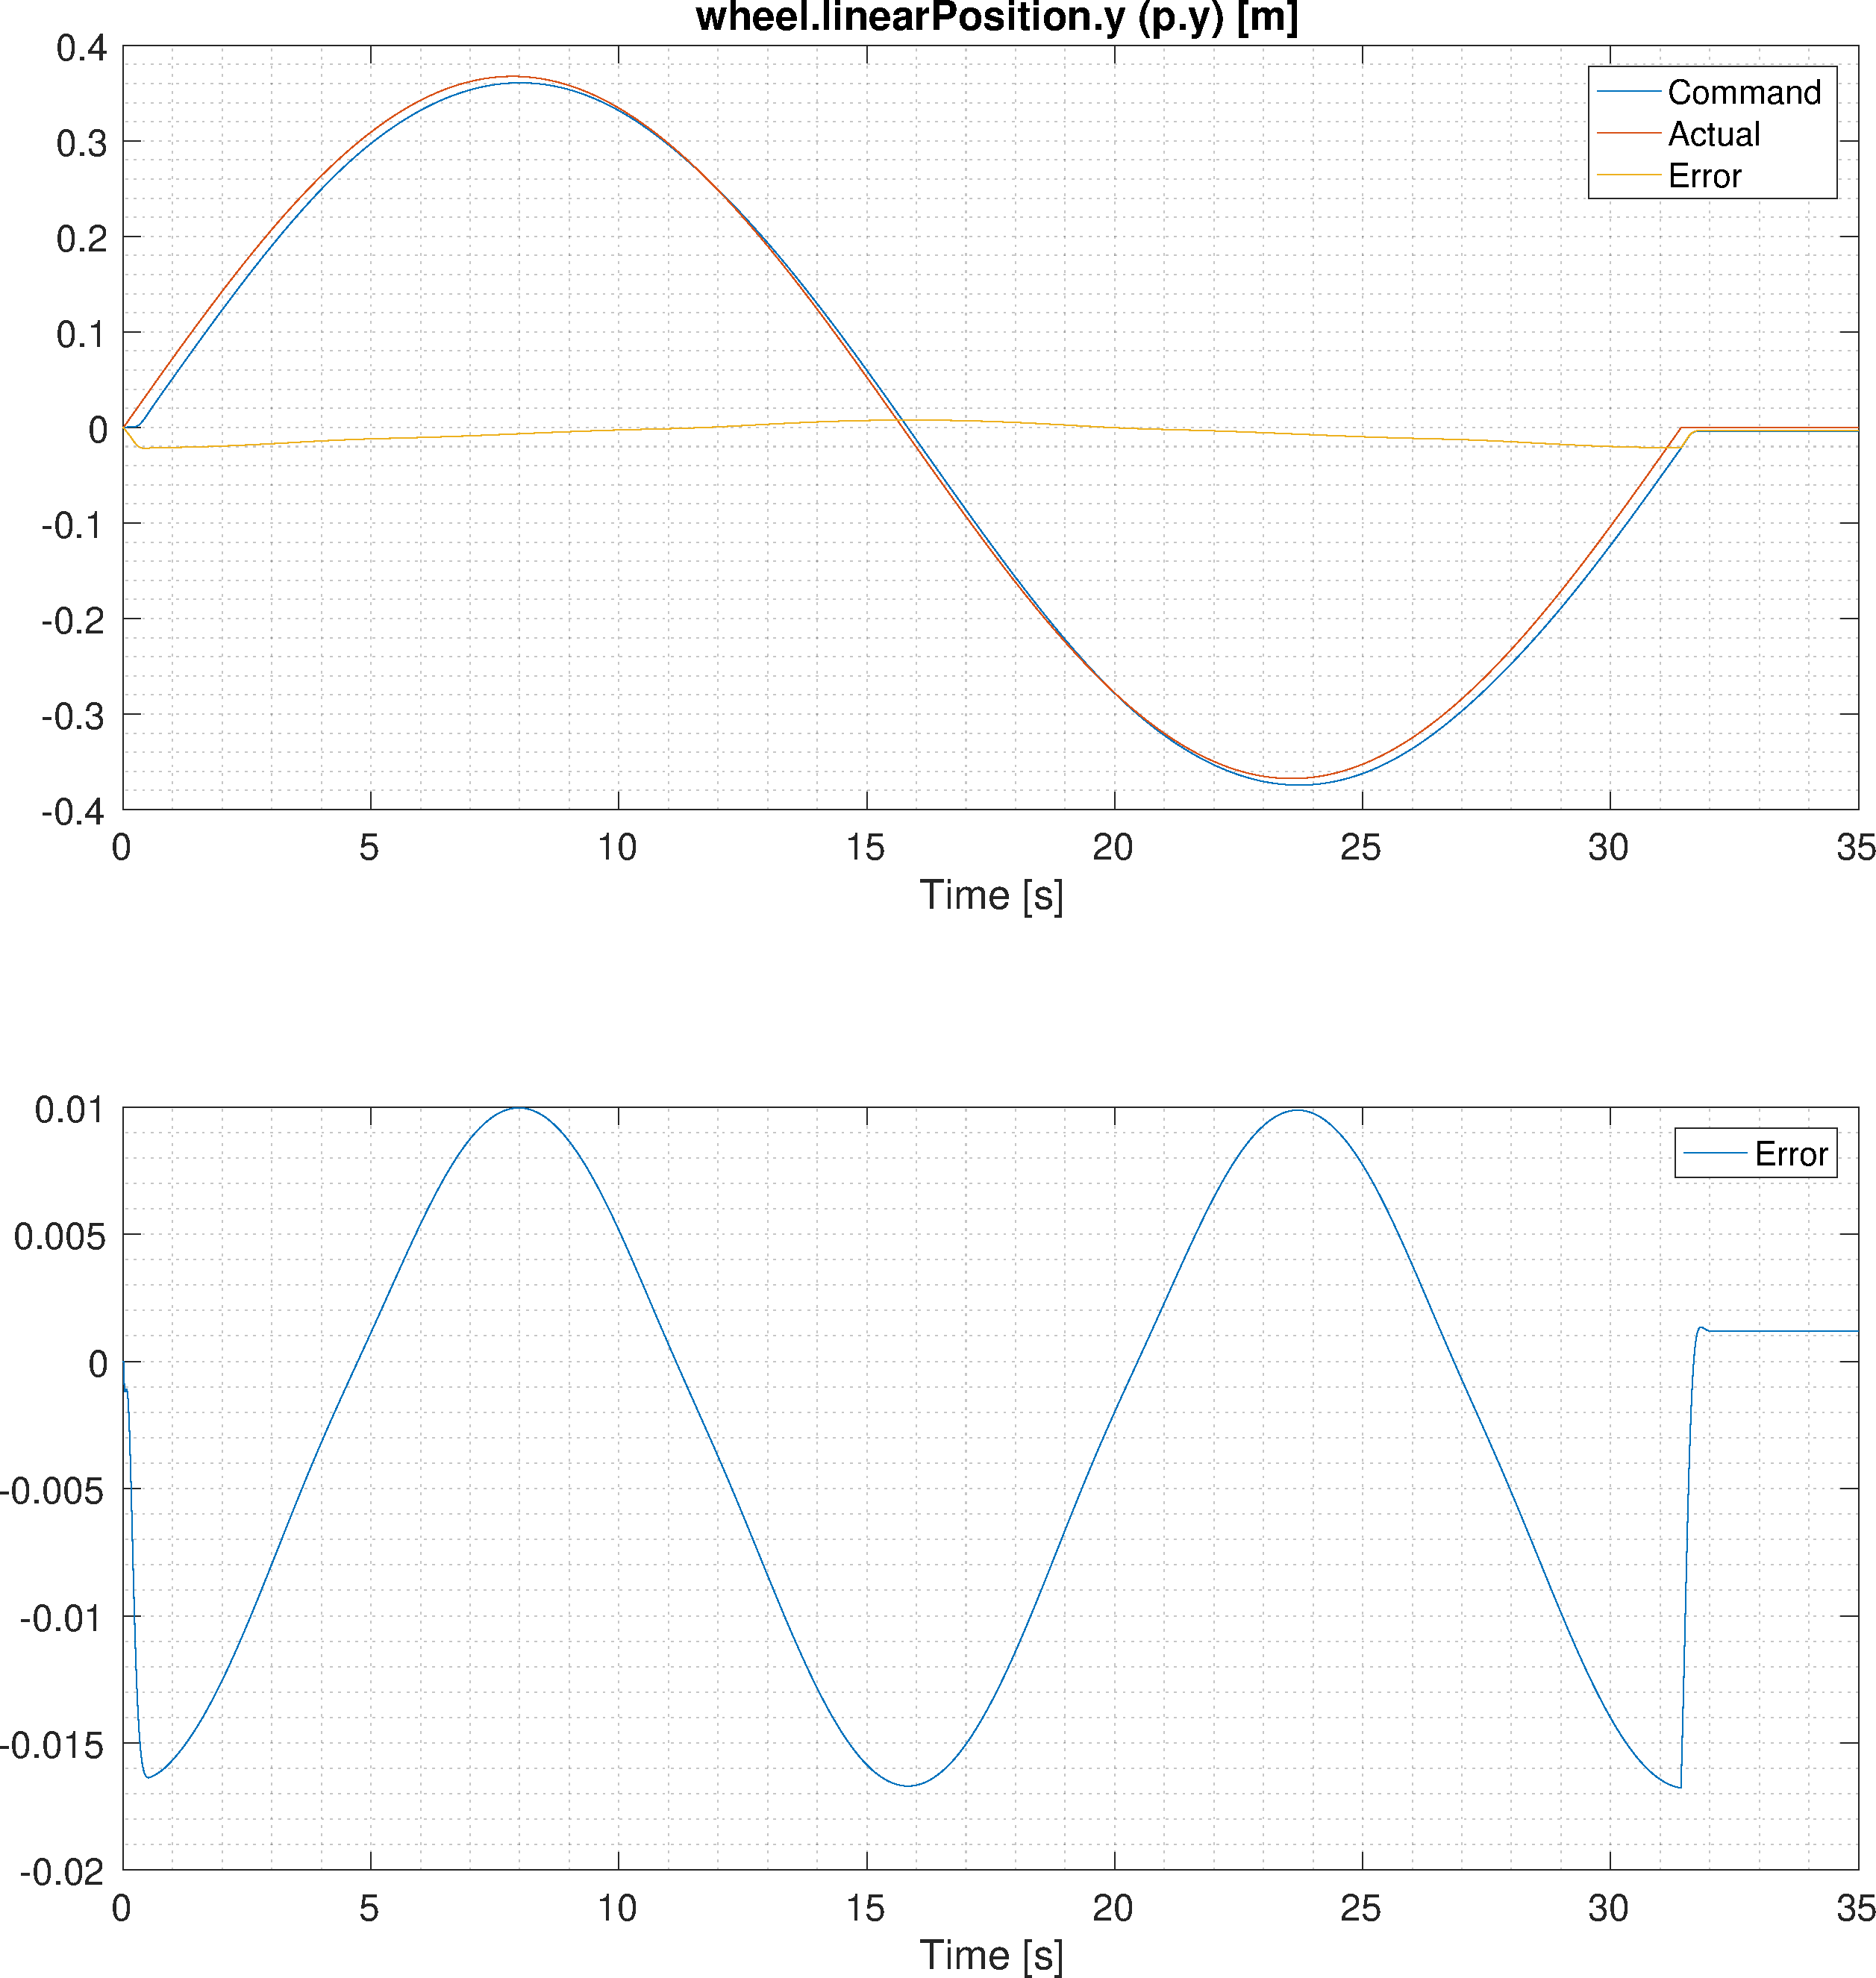
\includegraphics[trim = 0em 0em 0em 0em, clip, width=0.975\textwidth]{p-y.pdf}%
\caption[{[Control Gains: LQR]: Simulation Results: Wheel Linear Position $p_{y}$}]%
        {{[Control Gains: LQR]: Simulation Results: Wheel Linear Position $p_{y}$%
          \label{FIG:controllerDesign:additionalDynamics:optimal:results:simulation:pY}%
        }}%
\end{figure}
\vspace*{\fill}




\clearpage





\vspace*{\fill}
\begin{figure}[H]%
\centering%
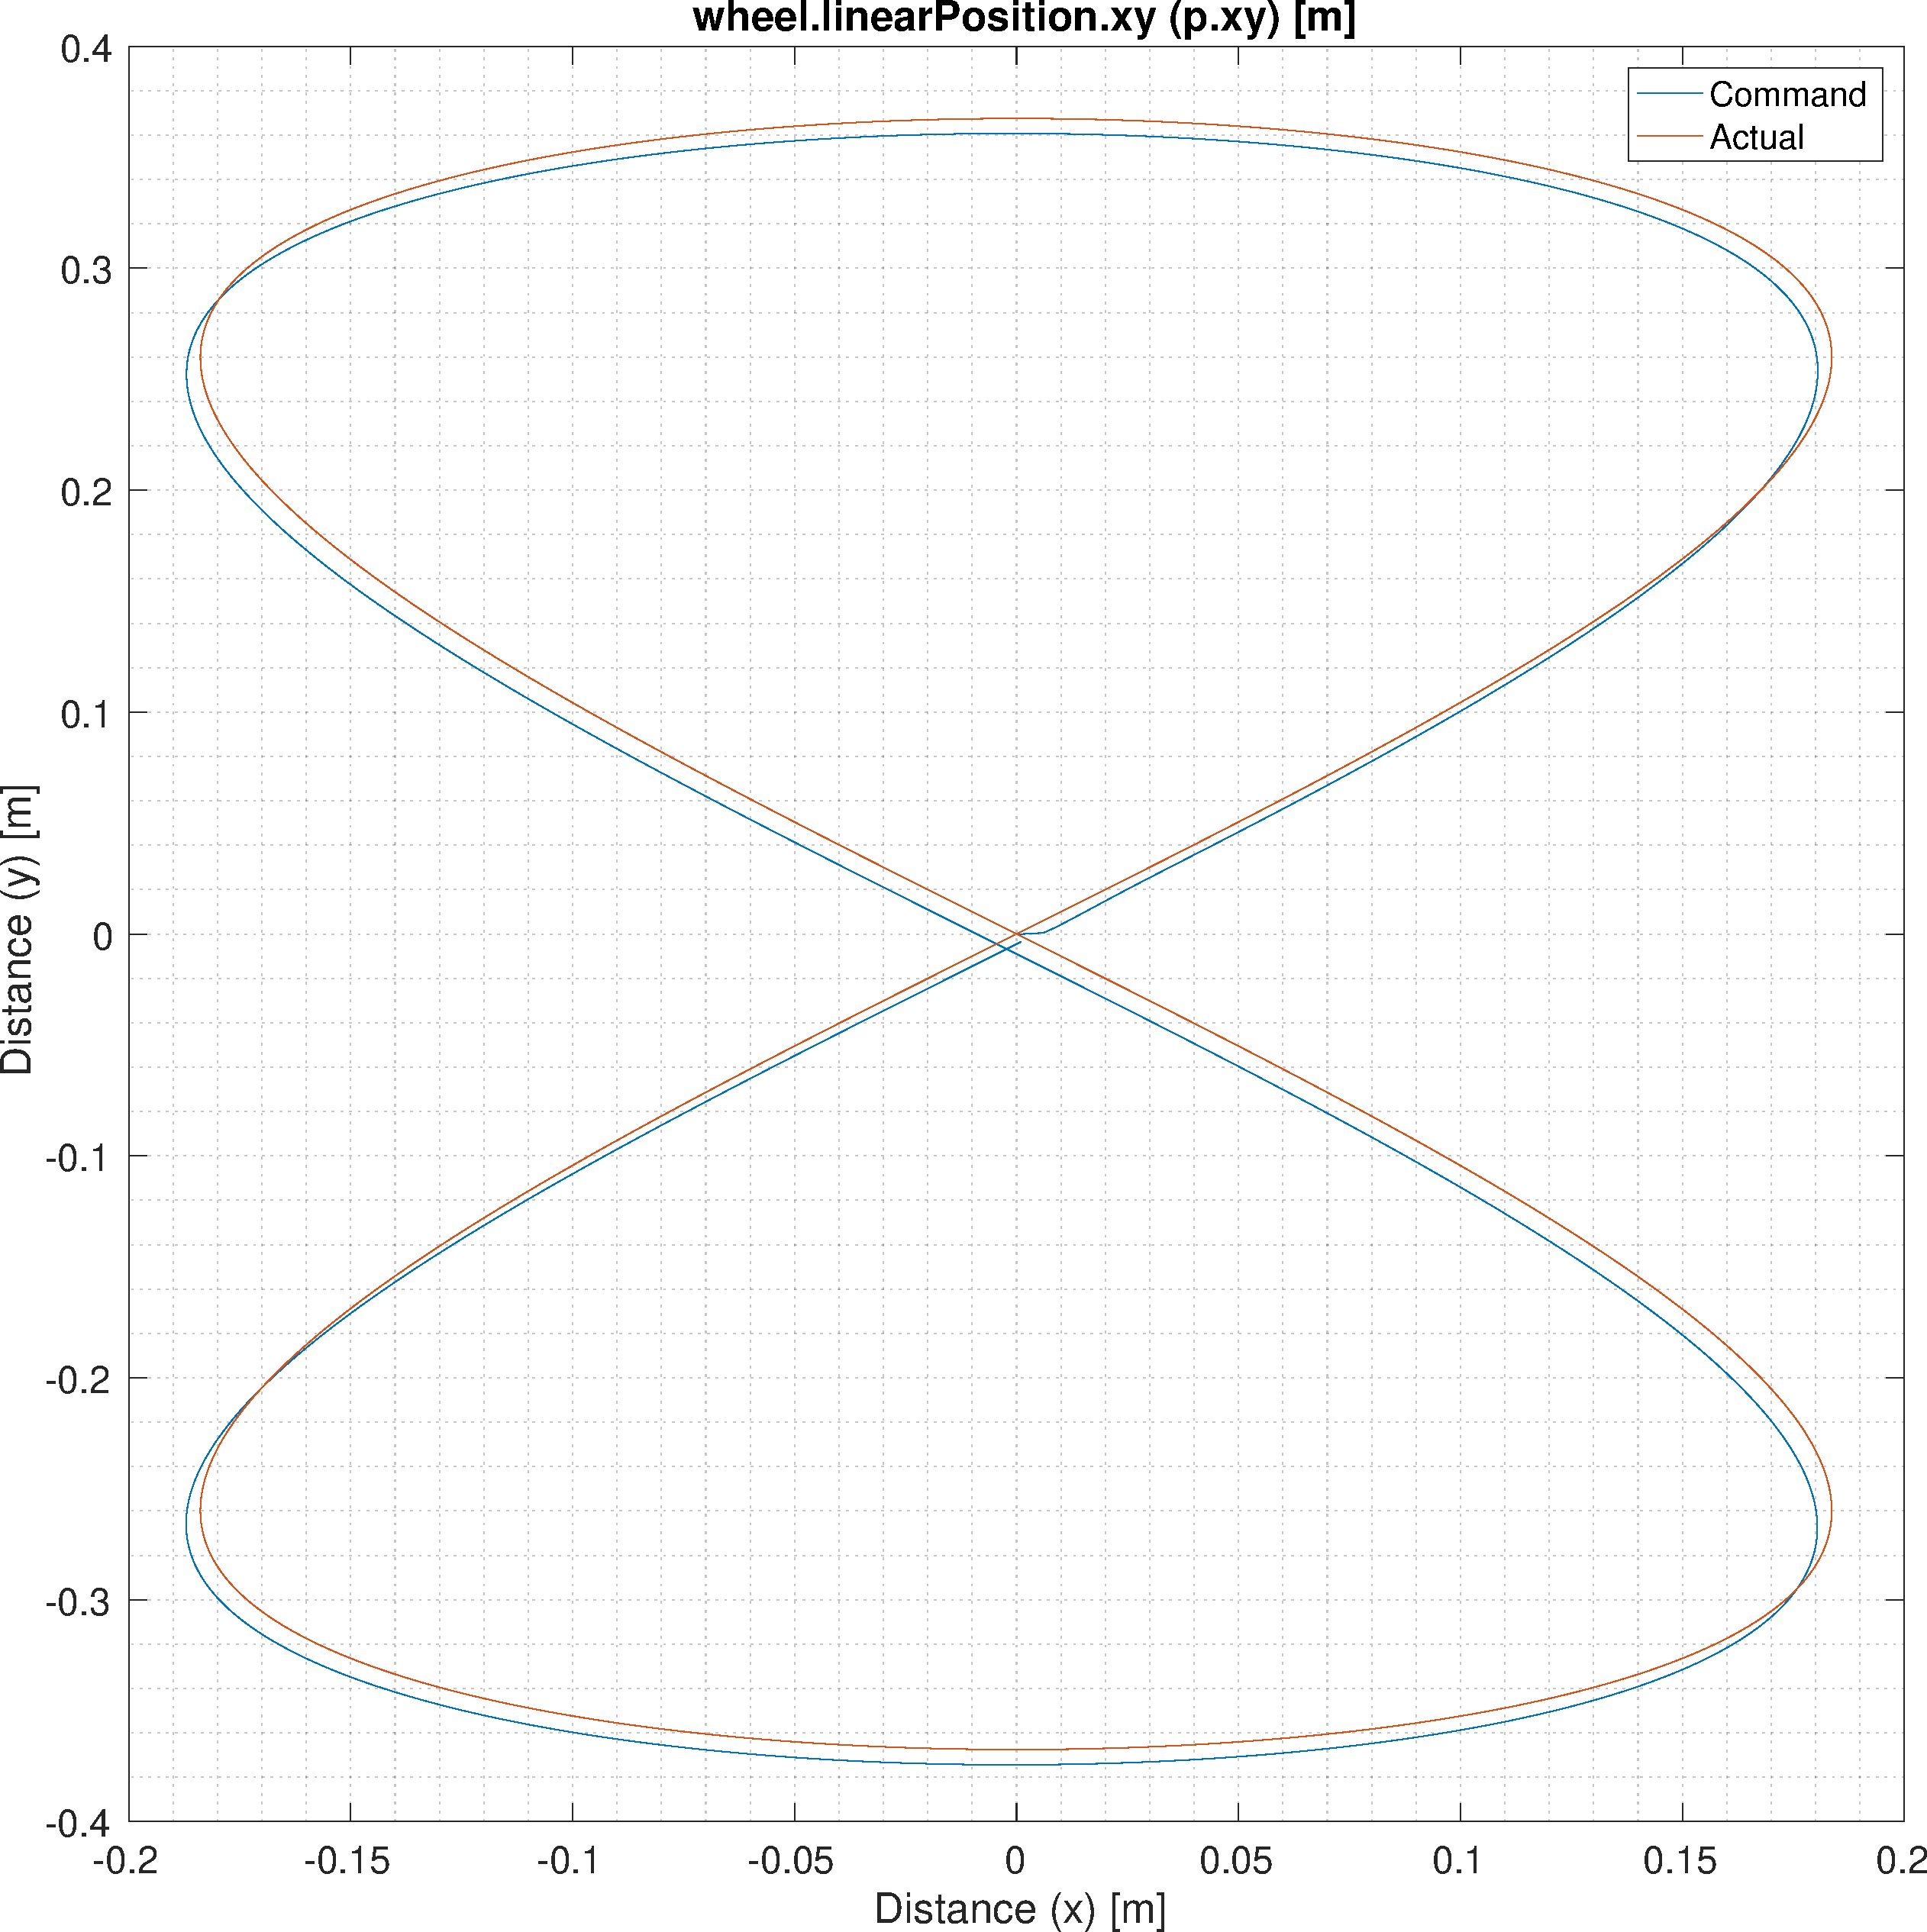
\includegraphics[trim = 0em 0em 0em 0em, clip, width=0.975\textwidth]{p-xy.pdf}%
\caption[{[Control Gains: LQR]: Simulation Results: Wheel Linear Position $p_{xy}$}]%
        {{[Control Gains: LQR]: Simulation Results: Wheel Linear Position $p_{xy}$%
          \label{FIG:controllerDesign:additionalDynamics:optimal:results:simulation:pXY}%
        }}%
\end{figure}
\vspace*{\fill}




\clearpage





\vspace*{\fill}
\begin{figure}[H]%
\centering%
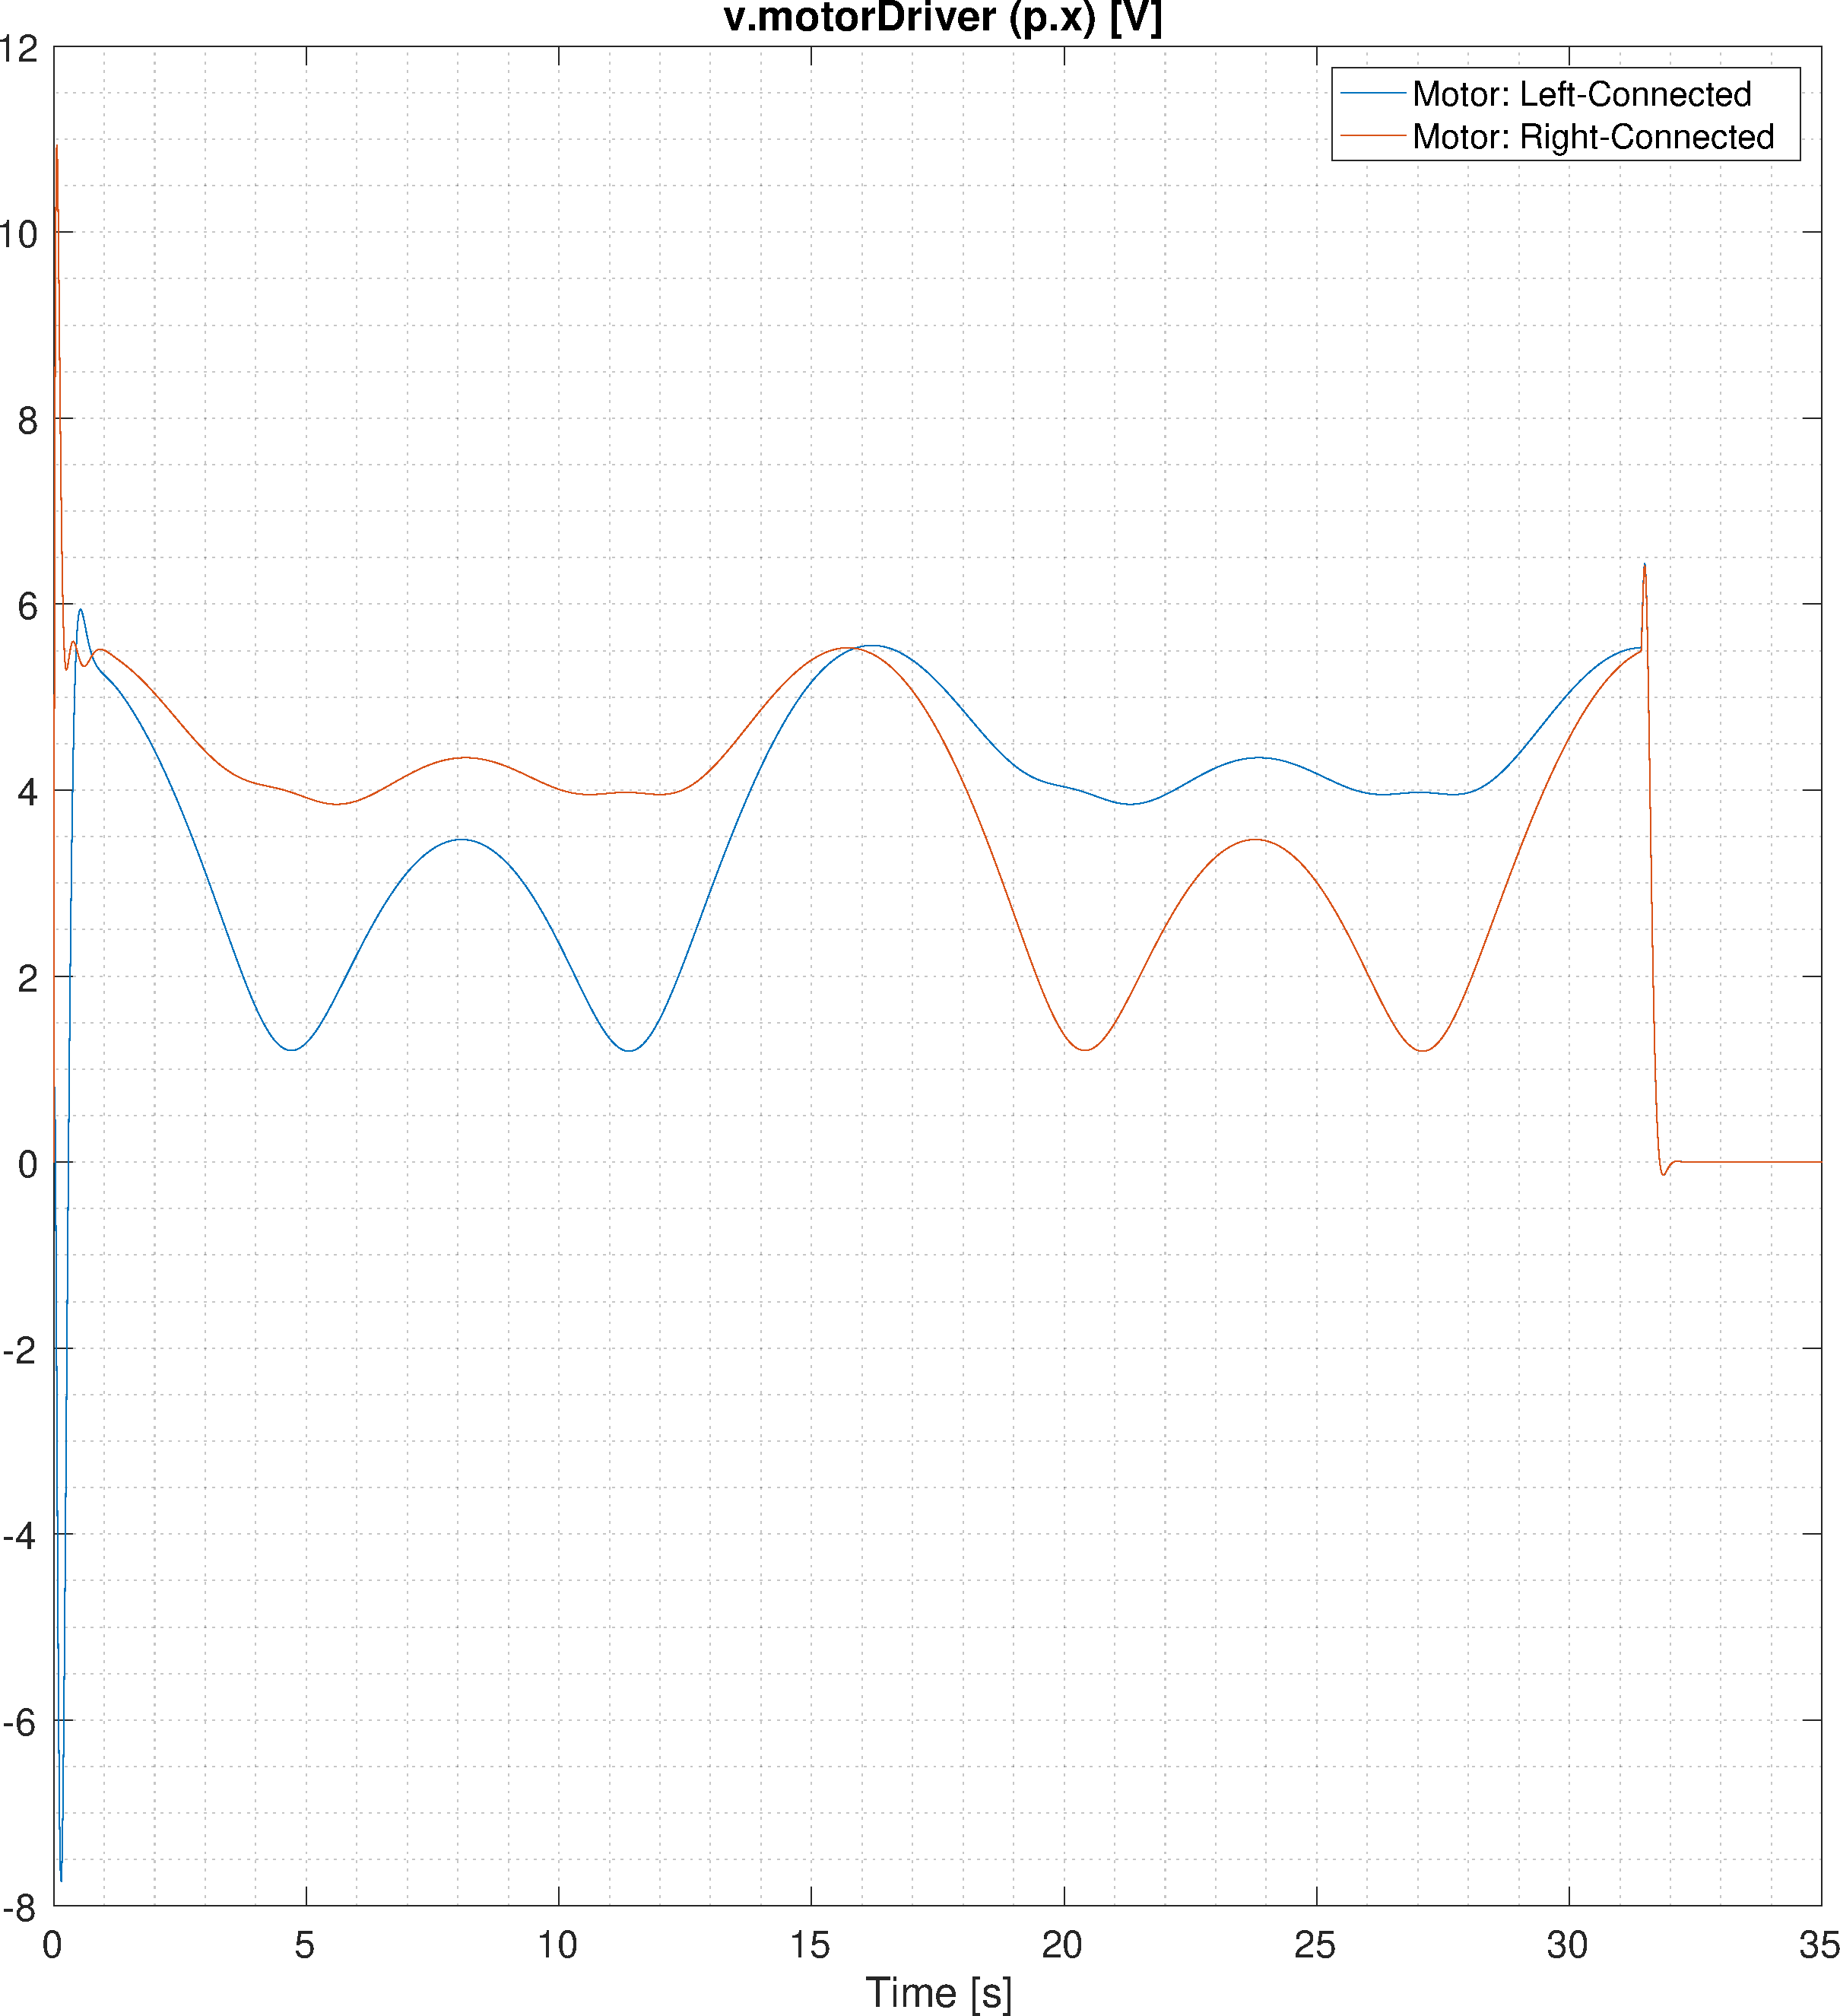
\includegraphics[trim = 0em 0em 0em 0em, clip, width=0.975\textwidth]{v-lm.pdf}%
\caption[{[Control Gains: LQR]: Simulation Results: Motor Driver Commanded Voltage $v_{motorDriver}$}]%
        {{[Control Gains: LQR]: Simulation Results: Motor Driver Commanded Voltage $v_{motorDriver}$%
          \label{FIG:controllerDesign:additionalDynamics:optimal:results:simulation:vMotorDriver}%
        }}%
\end{figure}
\vspace*{\fill}




\clearpage







%\subsubsubsection{Hardware Implementation}






\clearpage




\iffalse

\subsubsection{Pole-Placement}

Several pole-placement techniques also exist
\cite{REF:textbook:1995-vaccaro}.
This section is representative of future work with the system.

\subsubsubsection{Background}
\subsubsubsection{Simulation Implementation}
\subsubsubsection{Hardware Implementation}




\clearpage

\fi




\end{document}












%\renewcommand{\sectionedEquation}{\thesection--\arabic{equation}}
%\counterwithout*{equation}{subsection}

\stopcontents[additionalDynamics]
%\addtocontents{toc}{\string\setcounter{tocdepth}{1}}




\end{document}











% !TEX TS-program = arara
%  arara: lmkclean
%  arara: pdflatex: {   draft: yes, options: '-file-line-error -halt-on-error' }
%  arara: biber
%  arara: pdflatex: {   draft: yes, options: '-file-line-error -halt-on-error' }
%  arara: pdflatex: { synctex: yes, options: '-file-line-error -halt-on-error' }
%  arara: lmkclean
\documentclass[crop=false,float=true,class=scrreprt]{standalone}

\providecommand{\main}{../..}
% Preamble
 \input{\main/Subfiles/0-Preamble/1-packages.tex}

 \input{\main/Subfiles/0-Preamble/2-userInput-graphicsPath.tex}

 \input{\main/Subfiles/0-Preamble/3-pageLayout.tex}


% Watermark
 \input{\main/Subfiles/0-Preamble/watermark.tex}

% Floats:
 \input{\main/Subfiles/0-Preamble/floatConfig.tex}
%\input{\main/Subfiles/0-Preamble/sectionNumberIncludedInFloatCounter.tex}

% Commands:
 \input{\main/Subfiles/0-Preamble/commonCommands.tex}
 \input{\main/Subfiles/0-Preamble/allsubsSections.tex}
 \input{\main/Subfiles/0-Preamble/changePageSize.tex}

% Bug Fixes:
 \input{\main/Subfiles/0-Preamble/nociteFix.tex}
  % Preamble [document configuration]

\begin{document}




\printbibliography[segment=\therefsegment, heading=subbibnumbered, title={References}]




\clearpage 




\end{document}













%\renewcommand{\sectionedEquation}{\thesection--\arabic{equation}}
%\counterwithout*{equation}{subsection}

\stopcontents[controlDesign]
%\addtocontents{toc}{\string\setcounter{tocdepth}{1}}




\end{document}










         %\addtocontents{toc}{\string\clearpage}
 % !TEX spellcheck = English (United States) (Aspell)
% !TEX TS-program = arara
%  arara: lmkclean
%  arara: pdflatex: {   draft: yes, options: '-file-line-error -halt-on-error' }
%  arara: biber
%  arara: pdflatex: {   draft: yes, options: '-file-line-error -halt-on-error' }
%  arara: pdflatex: { synctex: yes, options: '-file-line-error -halt-on-error' }
%  arara: lmkclean
\documentclass[crop=false,float=true,class=scrreprt]{standalone}

\providecommand{\main}{../..}
% Preamble
 % meta tools
\usepackage{standalone}                 % allows for independent runs of subfiles. [includes currfile].
                                        % IMPORTANT: [realmainfile] option of currfile requires compiler option -recorder to be active.
                                        % IMPORTANT: standalone loads currfile package without options.  To configure currfile options:
                                        %            place them in \documentclass[options](standalone) options. 
                                        %      NOTE: Loading the currfile package with options will clash with the standalone package.
\usepackage{etoolbox}                   % allows if/else statements in code. [required for: standalone+nocite fix, equation numbering.]

% math
\usepackage{mathtools}                  % includes amsmath, supplements it.
\usepackage{subdepth}                   % allows manual vertical alignment for misaligned subscripts.

% font
\newcommand{\xLanguage}{american}       % do not remove: used in multiple locations.
\usepackage[\xLanguage]{babel}          % hyphenates words correctly, based on document language. [\xlanguage is defined immediately above.]
\usepackage{amssymb}                    % symbols. [permits use of \bigstar].
%\usepackage{mathptmx}                  % times new roman font. totally lame, but required by EB. [supercedes 'times' package].
\usepackage[T1]{fontenc}                % improves pdf reader's ability to copy    atypical text characters from output pdf file.
\usepackage[latin1]{inputenc}           % improves tex editor's ability to compile atypical text characters into output pdf file from tex file.

%\usepackage{verbatim}                  % [superceded by listings] improves verbatim environment. [includes comment package].
\usepackage{listings}                   % improved version of verbatim. imports script languages (with syntax coloring).

\usepackage{color}                      % color commands.
\usepackage[dvipsnames]{xcolor}         % additional color commands.

\usepackage{soul}                       % strikethrough commands.
\usepackage{transparent}                % transparent objects/font.

% layout: page/spacing/headings
\usepackage{geometry}                   % margin/page layout settings.
\usepackage{changepage}                 % allows adjustwidth, for figures larger than the margins.
\usepackage{pdflscape}                  % landscape page layout.
\usepackage{scrlayer-scrpage}           % improved header commands. [supercedes `fancyhdr' package].

\usepackage{eso-pic}                    % watermarks. [xwatermark is not compatible with scrpage. draftwatermark is not included with Tex Live.]

 \usepackage{setspace}                  % line spacing (allows \doublespacing). <-- not for urithesis
%\usepackage{parskip}                   % [superceded by KOMA]. tidies spacing. 

%\usepackage{titlesec}                  % [superceded by KOMA]. change style of all page      headers, etc.
%\usepackage{sectsty}                   % [superceded by KOMA]. change style of all sectional headers, etc.
\usepackage[toc,page]{appendix}         % appendices. [toc adds Appendices to TOC, page adds a page listed Appendices in the document.]

% references
\usepackage{chngcntr}                   % allows changes mid-document to section depth of equation counter reset.
\usepackage[titles]{tocloft}            % allows new lists such as \listofequations and \listoflistings.
                                        % Note: titles option permits header on table of contents and list of figures/tables/etc pages.
\usepackage{titletoc}                   % allows sub-[tables of contents]. allows increased margin between numbers and labels in toc.
                                        % IMPORTANT: [breaks \section* commands. use \setcounter{secnumdepth}{0} instead.]

% floats: figures/tables/lists
\usepackage{float}                      % improves floating objects (graphics/tables).

\usepackage{graphics}
\usepackage{graphicx}                   % graphics incorporation.
\usepackage{wrapfig}                    % allows text wrapping of figures.
\usepackage{subcaption}                 % allow captions with the subcaption command. [automatically loads caption package.]

\usepackage{tabu}                       % improved table commands.
\usepackage{longtable}                  % allows multipage tables.
\usepackage{multirow}                   % multirow command.
\usepackage{bigstrut}                   % bigstrut command. adds slight space up [t], down [b], or both. try next to \hline.
\usepackage{booktabs}                   % improved hline spacing commands in tables.

\usepackage{enumitem}                   % improved alterations to indent in enumerate/itemize. allows enumerate counter nesting.

% references
\usepackage{csquotes}                   % required for biblatex when using babel.
\usepackage{xpatch}                     % required for ieee-style @online no-date fix.

\usepackage[ backend      = biber       % supercedes bibtex
           , sorting      = none        % none: entries appear in order of \cite use
           , refsegment   = chapter     % restart numbering at beginning of each chapter
           , defernumbers = true,       % required for added global bibliography
           , style        = ieee        % ieee style
%          , doi          = false       % false for ieee style?
%          , isbn         = false       % false for ieee style?
           , citestyle    = numeric,    % \cite{REF:A, REF:B} => [1,2] instead of the default => [1], [2]
           , url          = true   ]
            {biblatex}                  % bibliographies (supercedes bibtex, biber, ...)

% hyperref                              % IMPORTANT: Always load hyperref last. It tends to break other packages when loaded first.
\usepackage[ hidelinks
           , linktoc   = all     ]
           {hyperref}                   % hyperlinks.












 %Setup Up Paths for Figures
\graphicspath{ %
             {\main/Figures/}                                % Directories for master file
             {\main/Figures/01-Intro/TitlePage/} 
             %
             {\main/Figures/02-Main/}
             {\main/Figures/02-Main/Verification/}
             %
             %
             }



 % Page size, margin, and header/footer settings:

% Enable "showframe" when editing margins
%\usepackage{showframe}                                            % Uncomment this to display header/footer/margins outlines.

% General margin settings:
 \newlength{\xhmargin   } \setlength  {\xhmargin   }{+1.000in    }
 \newlength{\xlmargin   } \setlength  {\xlmargin   }{\xhmargin   }
%                         \addtolength{\xlmargin   }{+0.500in    } % Include this row for additional margin for paper binding.
 \newlength{\xrmargin   } \setlength  {\xrmargin   }{\xhmargin   }
  
 \newlength{\xtmargin   } \setlength  {\xtmargin   }{+1.000in    } % Actual  tmargin = [\xtmargin - \xheadheight] = [0.500in] 
 \newlength{\xbmargin   } \setlength  {\xbmargin   }{+1.000in    } % Actual  bmargin = [\xbmargin - \xfootskip  ] = [0.500in] 

% Header  margin settings:
 \newlength{\xheadheight} \setlength  {\xheadheight}{+0.500in    } % May need to adjust tmargin in addition to this.
 \newlength{\xheadsep   } \setlength  {\xheadsep   }{+1.000em    }

% Footer  margin settings:
 \newlength{\xfootheight} \setlength  {\xfootheight}{+0.500in    } % May need to adjust bmargin in addition to this.
 \newlength{\xfootskip  } \setlength  {\xfootskip  }{\xfootheight} % Actual footskip = [\xfootheight - 1em + desired footsep] = [0.500in]
                          \addtolength{\xfootskip  }{-1.000em    } % <-- do not edit
                          \addtolength{\xfootskip  }{+1.000em    } % <-- do     edit: desired footsep



\KOMAoptions{headheight    = \xheadheight,
             footheight    = \xfootheight,
             DIV           = current,
             fontsize      = 10pt,
             parskip       = half-,
             toc           = chapterentrydotfill,
           % headings      = small,
           % headings      = openany,
             headings      = twolinechapter}

\geometry{letterpaper,
          tmargin       = \xtmargin,
          bmargin       = \xbmargin,
          lmargin       = \xlmargin,
          rmargin       = \xrmargin,
          headsep       = \xheadsep,
          footskip      = \xfootskip}

\savegeometry{default}




% Initialize double-spacing
\doublespacing




% Section headings

%\setkomafont{sectioning}   {\bfseries}
%\setkomafont{chapter}      {\nms}
%\setkomafont{section}      {\nms}
%\setkomafont{subsection}   {\nms}
%\setkomafont{subsubsection}{\nms}
%\setkomafont{paragraph}    {\nms}
%\setkomafont{subparagraph} {\nms}

\RedeclareSectionCommands[font       =  \nms,
                          beforeskip =  0pt,            % vspace before  chapter heading
                          innerskip  = -\parskip,       % vspace between chapter heading lines
                          afterskip  =  1\baselineskip] % vspace after   chapter heading
                         {chapter}
                         
\RedeclareSectionCommands[font       =  \nms,
                          afterskip  =  0.001em] % 0em puts the text inline with the heading. >.<
                          {section,subsection,subsubsection,paragraph,subparagraph}

% Make the word Chapter uppercase (but not the section heading label)
% Add a visible horizontal line
\renewcommand*{\chapterformat}{%
  \MakeUppercase{\chapappifchapterprefix{\nobreakspace}}\thechapter\autodot%
    \IfUsePrefixLine{%
        \par\nobreak\vspace*{-\parskip}\vspace*{-.6\baselineskip}%
        \rule{0.75\textwidth}{.5pt}%
}{\enskip}}%


\renewcommand\raggedchapter{\centering}


% Initialize headers and footers

\setkomafont{pageheadfoot}{\normalfont\normalcolor}

% Header: Center:
\chead{\fns}

% Footer: Center:
\cfoot{\thepage}

% Footer: Right-Side:
\ofoot{\fns}

% Header/footer enable/disable switch
\newpairofpagestyles{trueempty}{}
%  Enable: \pagestyle{scrheadings} [this is the default.]
% Disable: \pagestyle{trueempty}




% Watermark
 % Initialize watermark

\iffalse % <-- [ \iffalse: disabled | \iftrue: enabled ]
\AddToShipoutPictureFG{ 

\raisebox{.5\paperheight}{
\begin{minipage}[c][\paperheight][c]{\paperwidth}
\centering
\rotatebox[origin=c]{45}{ 
\scalebox{15}{ 
\transparent{0.35} \color{gray} D\sc{raft}
} } 
\end{minipage}
}

}
\fi


































% Floats:
 % Names of [float] and List of [float]

% Allow multiline captions to be centered.
\captionsetup{format=plain, justification=centering}




%-List of Contents
\expandafter\addto\csname captions\xLanguage\endcsname{% This line is needed when using the babel package.
  \renewcommand{\contentsname}{Table of Contents}%      % \xLanguage is defined in [1-packages.tex] near babel package.
                                                      }%  Renames Contents to List of Contents      

%-List of Code Listings
\renewcommand{\lstlistingname}    {Code Listing}              % Rename ``Listing'' floats to ``Code Listing'' floats.
\renewcommand{\lstlistlistingname}{List of \lstlistingname s \vspace{+0.40em}}








% Settings for importing scripts [listings package]


\lstset{ %
   backgroundcolor  = \color{white},     % choose the background color; you must add \usepackage{color} or \usepackage{xcolor}
   basicstyle       = \footnotesize,     % the size of the fonts that are used for the code
   breakatwhitespace= false,             % sets if automatic breaks should only happen at whitespace
   breaklines       = true,              % sets automatic line breaking
   captionpos       = tb,                % sets the caption-position
   commentstyle     = \color{Green},     % comment style
   deletekeywords   = {...},             % if you want to delete keywords from the given language
   escapeinside     = {\%*}{*)},         % if you want to add LaTeX within your code
   extendedchars    = true,              % lets you use non-ASCII characters; for 8-bits encodings only, does not work with UTF-8
   frame            = single,            % adds a frame around the code
   keepspaces       = true,              % keeps spaces in text, 
                                         %   useful for keeping indentation of code (possibly needs columns=flexible)
   keywordstyle     = \color{blue},      % keyword style
   language         = Matlab,            % the language of the code
   morekeywords     = {*,...},           % if you want to add more keywords to the set
   numbers          = left,              % where to put the line-numbers; possible values are (none, left, right)
   numbersep        = 5pt,               % how far the line-numbers are from the code
   numberstyle      = \tiny\color{gray}, % the style that is used for the line-numbers
   rulecolor        = \color{black},     % if not set, the frame-color may be changed on line-breaks within 
                                         %   not-black text (e.g. comments (green here))
   showspaces       = false,             % show spaces everywhere adding particular underscores; it overrides 'showstringspaces'
   showstringspaces = false,             % underline spaces within strings only
   showtabs         = false,             % show tabs within strings adding particular underscores
   stepnumber       = 1,                 % the step between two line-numbers. If it's 1, each line will be numbered
   stringstyle      = \color{purple},    % string literal style
   tabsize          = 2,                 % sets default tabsize to 2 spaces
   title            = \lstname           % show the filename of files included with \lstinputlisting; also try caption 
                                         %   instead of title
}















%% Sectioned Float Counters:

% Required Packages:
% - chngcntr
% - etoolbox
% - listings
% - titletoc


% Save a copy of the original float counters.
\let\xtheequationOriginal\theequation
\let\xthefigureOriginal\thefigure
\let\xthetableOriginal\thetable
\let\xthelstlistingOriginal\thelstlisting




% Command: Sectioned Counter

\newcommand{\sectionedCounter}     [1]
  % Input #1: section, subsection, subsubsection, paragraph, subparagraph, or \determineSection
  %
  %-This command configures all float counters to reset when switching to 
  %   a new section at (or above) a user-specified depth.
  % Reuse of the command overwrites the previous reset flags.
  %
  %-This command prepends all float counters with the current section number 
  %  (at the user-specified depth).
{
  \counterwithout*{equation}  {section} 
  \counterwithout*{figure}    {section}
  \counterwithout*{table}     {section}
  \counterwithout*{lstlisting}{section}
    
  \counterwithout*{equation}  {subsection} 
  \counterwithout*{figure}    {subsection}
  \counterwithout*{table}     {subsection}
  \counterwithout*{lstlisting}{subsection}
    
  \counterwithout*{equation}  {subsubsection} 
  \counterwithout*{figure}    {subsubsection}
  \counterwithout*{table}     {subsubsection}
  \counterwithout*{lstlisting}{subsubsection}
    
  \counterwithout*{equation}  {paragraph} 
  \counterwithout*{figure}    {paragraph}
  \counterwithout*{table}     {paragraph}
  \counterwithout*{lstlisting}{paragraph}
    
  \counterwithout*{equation}  {subparagraph} 
  \counterwithout*{figure}    {subparagraph}
  \counterwithout*{table}     {subparagraph}
  \counterwithout*{lstlisting}{subparagraph}

  \counterwithin*{equation}  {#1}   % Reset counter whenever there is a new \section
  \counterwithin*{figure}    {#1}
  \counterwithin*{table}     {#1}
  \counterwithin*{lstlisting}{#1}   % The listings counter is not actually defined until \AtBeginDocument. 
                                    % Thus, if using this command (including listings) within the preamble, 
                                    %   use ``\AtBeginDocument{\sectionedCounter{<input>}}'' instead.

  \renewcommand{\theequation  }{\sectionedCounterStyle{#1}{equation}}
  \renewcommand{\thefigure    }{\sectionedCounterStyle{#1}{figure}}
  \renewcommand{\thetable     }{\sectionedCounterStyle{#1}{table}}
  \renewcommand{\thelstlisting}{\sectionedCounterStyle{#1}{lstlisting}}  
}


\newcommand{\sectionedCounterStyle}[2]
% Input #1: section, subsection, subsubsection, paragraph, subparagraph
% Input #1: equation, lstlisting, table, figure
%
%-This command sets the syntax of float counters.
%
%-This command prepends the float counter number with a section number (at a user defined depth).
%-This command separates the float number and the section number with an en–dash.
%
%-This command takes <float> rather than \the<float> such that the input of \sectionedCounter may be used.
%
% Example:  Using \sectionedCounterStyle{subsection}{figure},
%           Figure~\ref{FIG:exampleFig} with the seventh figure in Section 1.3.4.5 outputs: Figure 1.3–7 .
{\csname the#1\endcsname--\arabic{#2}}

%{\csname the#1\endcsname--\ifnum\value{#2}<10 0\fi\arabic{#2}} <-- Method to zero pad the float number.



% Provide extra \hspace in Lists of <Float>s for the increased number of characters in the counters.
\newlength{\xtocmargin    } \setlength{\xtocmargin    }{3.5em}
\newlength{\xtoclabelwidth} \setlength{\xtoclabelwidth}{3.5em}
\newlength{\xlsttocmargin } \setlength{\xlsttocmargin }{0.0em} % Needs to be \xtoclabelwidth - \xtocmargin.


%\dottedcontents{section}[margin from leftmargin]{above-code}{label width}{leader width}
 \dottedcontents{figure}[\xtocmargin]{}{\xtoclabelwidth}{1pc}     % No spaces allowed.
 \dottedcontents {table}[\xtocmargin]{}{\xtoclabelwidth}{1pc}     % No spaces allowed.

\makeatletter
\renewcommand*{\l@lstlisting}[2]{\@dottedtocline{1}{\xlsttocmargin}{\xtoclabelwidth}{#1}{#2}}
\makeatother




% Set float counters to include their full section number.
\AtBeginDocument{\sectionedCounter{subsection}}

% Recall:
% The listings counter is not actually defined until \AtBeginDocument. 
% Thus, if using this command (including listings) within the preamble, 
%   use ``\AtBeginDocument{\sectionedCounter{<input>}}'' instead.

% Command: Determine Section
\newcommand{\determineSection}{%  [Provides full section counter of current section, independent of the section depth.]
  \ifnum\value{subsubsection} > 0%
  \ifnum\value{paragraph}     > 0% 
  \ifnum\value{subparagraph}  > 0 paragraph%
  \else subsubsection\fi%
  \else subsection\fi%
  \else section\fi%
}

































% Commands:
 % Command: Multicol / Multirow
\newcommand{\mc}	[3]	{\multicolumn{#1}{#2}{#3}}                 % Abbreviates multicolumn. [n.col][ alignments ][content]
\newcommand{\mr}	[3]	{\multirow{#1}{#2}{#3}}                    % Abbreviates multirow   . [n.row][width(use *)][content]

% Command: Font Changes
\newcommand{\Hgs}          {\Huge}                                   % Abbreviates Huge     size     font command.
\newcommand{\hgs}          {\huge}                                   % Abbreviates huge     size     font command.
\newcommand{\LGs}          {\LARGE}                                  % Abbreviates LARGE    size     font command.
\newcommand{\Lgs}          {\Large}                                  % Abbreviates Large    size     font command.
\newcommand{\lgs}          {\large}                                  % Abbreviates large    size     font command.

\newcommand{\nms}          {\normalsize}                             % Abbreviates normal   size     font command.
\newcommand{\sms}          {\small}                                  % Abbreviates small    size     font command.
\newcommand{\fns}          {\footnotesize}                           % Abbreviates footnote size     font command.
\newcommand{\scs}          {\scriptsize}                             % Abbreviates script   size     font command.

\newcommand{\tnf}	[1]	{\textnormal{#1}}                         % Abbreviates text   normal     font command.
\newcommand{\tbf}	[1]	{\textbf{#1}}                             % Abbreviates text   bold       font command.
\newcommand{\tif}	[1]	{\textit{#1}}                             % Abbreviates text   italics    font command.
\newcommand{\tuf}	[1]	{\ul{#1}}                                 % Abbreviates text   underline  font command.
\newcommand{\ttt}	[1]	{\texttt{#1}}                             % Abbreviates text   teletype   font command. [monospace font.]

\newcommand{\sbf}	[1]	{\boldsymbol{#1}}                         % Abbreviates symbol bold       font command.
\newcommand{\mbf}	[1]	{\mathbf{#1}}                             % Abbreviates math   bold       font command.
\newcommand{\mrm}	[1]	{\mathrm{#1}}                             % Abbreviates math   roman      font command.


































 % Section numbering: Table of contents and section depth
\newcounter{xTocdepth}    \setcounter{xTocdepth}   {2} % These are used in multiple locations.
\newcounter{xSecnumdepth} \setcounter{xSecnumdepth}{5} % These are used in multiple location.

\setcounter{tocdepth}    {\thexTocdepth}
\setcounter{secnumdepth} {\thexSecnumdepth}




% Command: Subsection 
% -[Interchange paragraph and subparagraph with their subsubsubparagraph and subsubsubsub paragraph equivalents].
\newcommand{\subsubsubsection}     [1] {                                \paragraph{#1}                                            }
\newcommand{\subsubsubsectionA}    [1] { \setcounter{secnumdepth}{0}    \paragraph{#1} \setcounter{secnumdepth}{\thexSecnumdepth} }
\newcommand{\paragraphA}           [1] { \setcounter{secnumdepth}{0}    \paragraph{#1} \setcounter{secnumdepth}{\thexSecnumdepth} }
\newcommand{\subsubsubsubsection}  [1] {                             \subparagraph{#1}                                            }
\newcommand{\subsubsubsubsectionA} [1] { \setcounter{secnumdepth}{0} \subparagraph{#1} \setcounter{secnumdepth}{\thexSecnumdepth} }
\newcommand{\subparagraphA}        [1] { \setcounter{secnumdepth}{0} \subparagraph{#1} \setcounter{secnumdepth}{\thexSecnumdepth} }


% Format paragraph and subparagraph exactly like subsection.
% -subsubsection is formatted like subsection by default.
\makeatletter

\renewcommand{\paragraph}               %
  {\@startsection{paragraph}{4}{\z@}    %
  {-2.5ex\@plus -1ex \@minus -.25ex}    %
  {1.25ex \@plus .25ex}                 %
  {\normalfont\sffamily\normalsize\bfseries}     }

\renewcommand{\subparagraph}            %
  {\@startsection{subparagraph}{5}{\z@} %
  {-2.5ex\@plus -1ex \@minus -.25ex}    %
  {1.25ex \@plus .25ex}                 %
  {\normalfont\sffamily\normalsize\bfseries}     }

\makeatother













 % Command: Change page size
\newcommand{\beginLargePage}[2]{
  %\pdfpagewidth  = 11in       % [\pdfpagewidth and \pdfpageheight are superceded by KOMAoptions].
  %\pdfpageheight = 17in
  \KOMAoptions{paper        = #1:#2        , % Inputs are measurements:
               pagesize                    , % Example A: \beginLargePage{11in}{17in}
               headheight   = \xheadheight , % Example B: \beginLargePage{08in}{14in}
               footheight   = \xfootheight ,
               DIV          = current      }
               
  \newgeometry{layoutwidth  = #1         ,
               layoutheight = #2         , 
               tmargin      = \xtmargin  ,
               bmargin      = \xbmargin  ,
               hmargin      = \xhmargin  ,
               headsep      = \xheadsep  ,
               footskip     = \xfootskip }
                            }




% Command: Revert page size
\newcommand{\stopLargePage}{
  %\pdfpagewidth  = 08.5in      % [\pdfpagewidth and \pdfpageheight are superceded by KOMAoptions].
  %\pdfpageheight = 11.0in
  \KOMAoptions{paper=8.5in:11in,pagesize,DIV=current}
  \restoregeometry
                           }

% Bug Fixes:
 \iffalse

% Allow \nocite with standalone package
\makeatletter
\def\@documentnocite#1{\@bsphack
  \@for\@citeb:=#1\do{%
    \edef\@citeb{\expandafter\@firstofone\@citeb}%
    \if@filesw\immediate\write\@auxout{\string\citation{\@citeb}}\fi
    \@ifundefined{b@\@citeb}{\G@refundefinedtrue
      \@latex@warning{Citation `\@citeb' undefined}}{}}%
  \@esphack}
\AtBeginDocument{\let\nocite\@documentnocite}
\makeatother
% [Ideally \nocite will be patched in a later distribution.]

\fi






































  % Preamble [document configuration]

\begin{document}




%\addtocontents{toc}{\string\setcounter{tocdepth}{2}}
\startcontents[testPlatform]

%\renewcommand{\sectionedEquation}{\thesubsection--\arabic{equation}}
%\counterwithin*{equation}{subsection}




\chapter{Test Platform}
\label{SEC:testPlatform}

\iffalse
\singlespacing%
\printcontents[testPlatform]{}{1}{%
  \addtocontents{ptc}{\string\setcounter{tocdepth}{5}}%
% 
  \subsection*{List of Contents}%
  \vspace*{+2em}
% \addcontentsline{toc}{subsection}{List of Contents}%
  }%
\doublespacing%
\clearpage
\fi

% !TEX TS-program = arara
%  arara: lmkclean
%  arara: pdflatex: {   draft: yes, options: '-file-line-error -halt-on-error' }
%  arara: biber
%  arara: pdflatex: {   draft: yes, options: '-file-line-error -halt-on-error' }
%  arara: pdflatex: { synctex: yes, options: '-file-line-error -halt-on-error' }
%  arara: lmkclean
\documentclass[crop=false,float=true,class=scrreprt]{standalone}

\providecommand{\main}{../../..}
% Preamble
 \input{\main/Subfiles/0-Preamble/1-packages.tex}

 \input{\main/Subfiles/0-Preamble/2-userInput-graphicsPath.tex}

 \input{\main/Subfiles/0-Preamble/3-pageLayout.tex}


% Watermark
 \input{\main/Subfiles/0-Preamble/watermark.tex}

% Floats:
 \input{\main/Subfiles/0-Preamble/floatConfig.tex}
%\input{\main/Subfiles/0-Preamble/sectionNumberIncludedInFloatCounter.tex}

% Commands:
 \input{\main/Subfiles/0-Preamble/commonCommands.tex}
 \input{\main/Subfiles/0-Preamble/allsubsSections.tex}
 \input{\main/Subfiles/0-Preamble/changePageSize.tex}

% Bug Fixes:
 \input{\main/Subfiles/0-Preamble/nociteFix.tex}
  % Preamble [document configuration]

\begin{document}




The test platform consists of the designated hardware,
{\fns[\tif{MinSeg M2V3 two-wheeled robot, see Section~\ref{SEC:preliminaryDecisions:selectHardware:minseg}}]},
and the designated development PC,
{\fns[\tif{see Section~\ref{SEC:preliminaryDecisions:selectHardware:developmentPC}}]}.
To interface with the hardware,
a Simulink model and a hierarchy of Matlab subscripts were created.

The Simulink model is capable of: 

\begin{itemize}[leftmargin=*, label=$\vcenter{\hbox{\tiny$\bullet$}}$, itemsep=-1em]

\item Acting as an algorithm with which to program the hardware, such that it may:
      \vspace*{-1em}
      \begin{itemize}[leftmargin=*, label=$\cdot$, itemsep=-1em]
      
      \item Process
      
      \item Actuate
      
      \item Communicate
      
      \end{itemize}

\item Simulate an equivalent model of "the hardware when loaded with the same algorithm".

\end{itemize}


The Matlab script hierarchy is capable of:

\begin{itemize}[leftmargin=*, label=$\vcenter{\hbox{\tiny$\bullet$}}$, itemsep=-1em]

\item Initialize model parameters.

\item Reconfigure model subsystems.

\item Initialize a build or simulate event.

\item Initialize a read or write event.

\item Post-process raw read data.

\item Save processed read data as well as other configuration data.

\item Plot processed read data.

\end{itemize}




\clearpage 




\end{document}











% !TEX spellcheck = English (United States) (Aspell)
% !TEX TS-program = arara
%  arara: lmkclean
%  arara: pdflatex: {   draft: yes, options: '-file-line-error -halt-on-error' }
%  arara: biber
%  arara: pdflatex: {   draft: yes, options: '-file-line-error -halt-on-error' }
%  arara: pdflatex: { synctex: yes, options: '-file-line-error -halt-on-error' }
%  arara: lmkclean
\documentclass[crop=false,float=true,class=scrreprt]{standalone}

\providecommand{\main}{../../..}
% Preamble
 \input{\main/Subfiles/0-Preamble/1-packages.tex}

 \input{\main/Subfiles/0-Preamble/2-userInput-graphicsPath.tex}

 \input{\main/Subfiles/0-Preamble/3-pageLayout.tex}


% Watermark
 \input{\main/Subfiles/0-Preamble/watermark.tex}

% Floats:
 \input{\main/Subfiles/0-Preamble/floatConfig.tex}
%\input{\main/Subfiles/0-Preamble/sectionNumberIncludedInFloatCounter.tex}

% Commands:
 \input{\main/Subfiles/0-Preamble/commonCommands.tex}
 \input{\main/Subfiles/0-Preamble/allsubsSections.tex}
 \input{\main/Subfiles/0-Preamble/changePageSize.tex}

% Bug Fixes:
 \input{\main/Subfiles/0-Preamble/nociteFix.tex}
  % Preamble [document configuration]

\begin{document}




%\addtocontents{toc}{\string\setcounter{tocdepth}{2}}
\startcontents[testPlatform:simulink]

%\renewcommand{\sectionedEquation}{\thesubsection--\arabic{equation}}
%\counterwithin*{equation}{subsection}




\section{Simulink: minseg\_M2V3\_2017a.slx}
\label{SEC:testPlatform:simulink}

% !TEX TS-program = arara
%  arara: lmkclean
%  arara: pdflatex: {   draft: yes, options: '-file-line-error -halt-on-error' }
%  arara: biber
%  arara: pdflatex: {   draft: yes, options: '-file-line-error -halt-on-error' }
%  arara: pdflatex: { synctex: yes, options: '-file-line-error -halt-on-error' }
%  arara: lmkclean
\documentclass[crop=false,float=true,class=scrreprt]{standalone}

\providecommand{\main}{../../..}
\input{\main/Subfiles/0-Preamble/0-Preamble.tex}  % Preamble [document configuration]

\begin{document}




The test platform consists of the designated hardware,
{\fns[\tif{MinSeg M2V3 two-wheeled robot, see Section~\ref{SEC:preliminaryDecisions:selectHardware:minseg}}]},
and the designated development PC,
{\fns[\tif{see Section~\ref{SEC:preliminaryDecisions:selectHardware:developmentPC}}]}.
To interface with the hardware,
a Simulink model and a hierarchy of Matlab subscripts were created.

The Simulink model is capable of: 

\begin{itemize}[leftmargin=*, label=$\vcenter{\hbox{\tiny$\bullet$}}$, itemsep=-1em]

\item Acting as an algorithm with which to program the hardware, such that it may:
      \vspace*{-1em}
      \begin{itemize}[leftmargin=*, label=$\cdot$, itemsep=-1em]
      
      \item Process
      
      \item Actuate
      
      \item Communicate
      
      \end{itemize}

\item Simulate an equivalent model of "the hardware when loaded with the same algorithm".

\end{itemize}


The Matlab script hierarchy is capable of:

\begin{itemize}[leftmargin=*, label=$\vcenter{\hbox{\tiny$\bullet$}}$, itemsep=-1em]

\item Initialize model parameters.

\item Reconfigure model subsystems.

\item Initialize a build or simulate event.

\item Initialize a read or write event.

\item Post-process raw read data.

\item Save processed read data as well as other configuration data.

\item Plot processed read data.

\end{itemize}




\clearpage 




\end{document}












\iffalse

\singlespacing%
\printcontents[testPlatform:simulink]{}{1}{%
  \addtocontents{ptc}{\string\setcounter{tocdepth}{5}}%
% 
  \subsection*{List of Contents}%
  \vspace*{+2em}
% \addcontentsline{toc}{subsection}{List of Contents}%
  }%
\doublespacing%
\clearpage

\fi

% !TEX TS-program = arara
%  arara: lmkclean
%  arara: pdflatex: {   draft: yes, options: '-file-line-error -halt-on-error' }
%  arara: biber
%  arara: pdflatex: {   draft: yes, options: '-file-line-error -halt-on-error' }
%  arara: pdflatex: { synctex: yes, options: '-file-line-error -halt-on-error' }
%  arara: lmkclean
\documentclass[crop=false,float=true,class=scrreprt]{standalone}

\providecommand{\main}{../../../..}
\input{\main/Subfiles/0-Preamble/0-Preamble.tex}  % Preamble [document configuration]
\begin{document}




\subsection{Root}
\label{SEC:testPlatform:simulink:root}

The top level of the model, also known as the model root,
is depicted in Figure~%
\ref{FIG:testPlatform:simulink:root}.

The model root is contains the three primary components of the system:

\begin{itemize}[leftmargin=*,itemsep=-1em]

\item Plant

\item Controller

\item Board Inputs and Outputs

\end{itemize}




\clearpage



\begin{landscape}
%\vspace*{\fill}
\begin{figure}[H]%
\centering%
%\fbox{%
\begin{minipage}[c][0.995\textheight][c]{0.995\linewidth}%
\centering%
\fbox{%
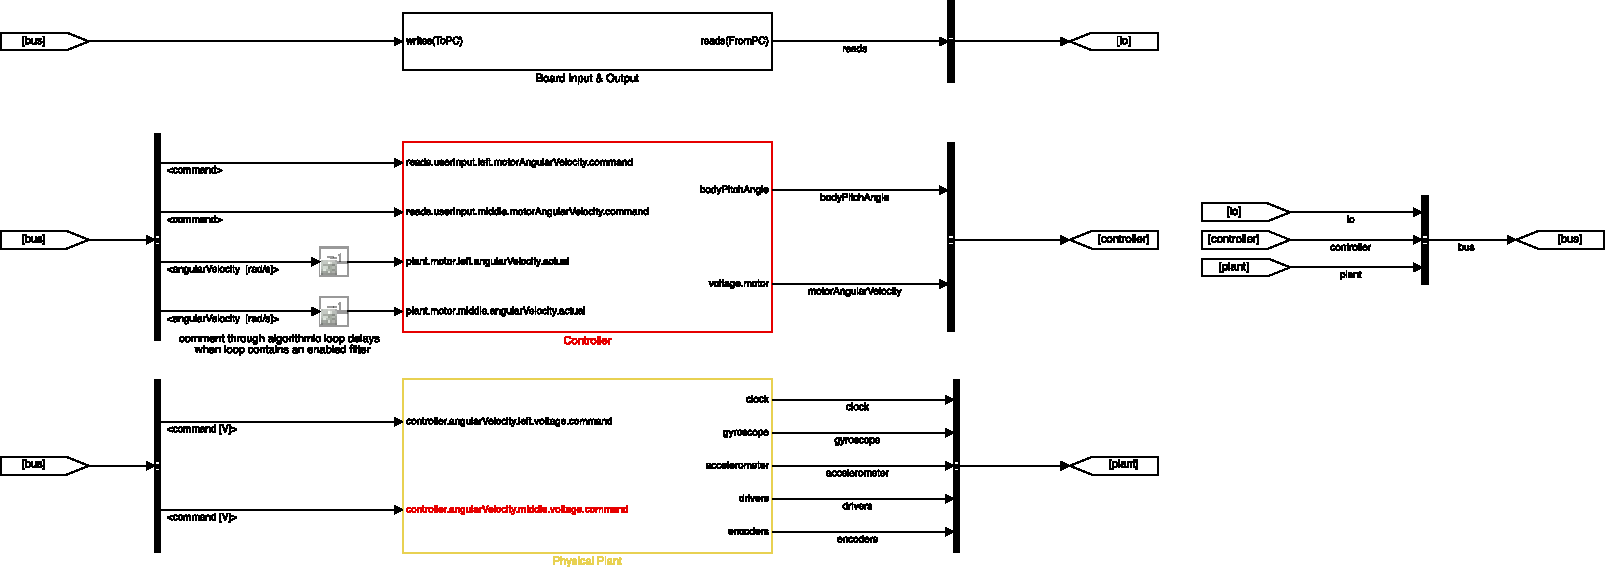
\includegraphics[trim = 0em 0em 0em 0em, clip, width=0.975\textwidth]{minseg_M2V3_2017a.pdf}%
}%
\caption[{[Simulink]: Root}]%
        {{[Simulink]: Root%
          \label{FIG:testPlatform:simulink:root}%
        }}%
\end{minipage}%
%}%
\end{figure}
%\vspace*{\fill}
\end{landscape}




\clearpage




\subsubsection{Bus Structures}
\label{SEC:testPlatform:simulink:root:bus}

Bus structures are a means of routing large quantities of signals.
They are similar to muxed signals; however, 
it is not necessary to separate all of the signals during the demux process.

It is evident in Figure~%
\ref{FIG:testPlatform:simulink:root}
that all of the components are passed into separate bus structures,
{\fns[\tif{black bars on the right-side of the figure}]},
and that those bus structures are in turn merged into one global bus structure.

This grants the user the ability to call any significant signal wherever it is needed
using bus selectors,
{\fns[\tif{black~bars on the left-side of the figure}]}.
The user should take care to implement a delay in the path of any signal which is implemented recursively
{\fns[\tif{as feedback}]}. 
{\fns[\tif{This prevents the formation of an algebraic loop}]}.




\subsubsection{Variant Subsystems}
\label{SEC:testPlatform:simulink:root:variant}

A variant subsystem is a subsystem containing multiple subsystems, defined as variants.
Only one variant can be active at one time.
The variant subsystem serves as the switch between them.
{\fns[\tif{Note that the variant subsystem cannot switch between variants during operation/runtime}]}.

Several subsystems contained in this model
%{\fns[\tif{but not appearing in Figure~\ref{FIG:testPlatform:simulink:root}}]},
are variant subsystems.
These variant subsystems are used to switch system configurations.
Examples of these variant configurations include:

\begin{itemize}[leftmargin=*,itemsep=0em, label=$\vcenter{\hbox{\tiny$\bullet$}}$]

\item The plant:
      \vspace{-1em}
      \begin{itemize}[leftmargin=*,itemsep=-1em, label=$\cdot$]
      
      \item Actual hardware drivers.
            \hspace*{\fill}{\fns[\tif{Hardware implementation only}.]}
      
      \item Hardware-equivalent simulation model of nonlinear dynamics.
            \hspace*{\fill}{\fns[\tif{Simulation only}.]}
            
      \item Hardware-equivalent simulation model of linear dynamics.
            \hspace*{\fill}{\fns[\tif{Simulation only}.]}
      
      \end{itemize}

\item The controller design:
      \vspace{-1em}
      \begin{itemize}[leftmargin=*,itemsep=-1em, label=$\cdot$]
      
      \item PID.
            \hspace*{\fill}{\fns[\tif{Primarily for initial hardware characterization}.]}
      
      \item Optimal.
      
      \item Pole-placement.
      
      \end{itemize}

\end{itemize}




\clearpage




\end{document}












\iffalse

% !TEX TS-program = arara
%  arara: lmkclean
%  arara: pdflatex: {   draft: yes, options: '-file-line-error -halt-on-error' }
%  arara: biber
%  arara: pdflatex: {   draft: yes, options: '-file-line-error -halt-on-error' }
%  arara: pdflatex: { synctex: yes, options: '-file-line-error -halt-on-error' }
%  arara: lmkclean
\documentclass[crop=false,float=true,class=scrreprt]{standalone}

\providecommand{\main}{../../../..}
\input{\main/Subfiles/0-Preamble/0-Preamble.tex}  % Preamble [document configuration]

\begin{document}




\subsection{Plant}
\label{SEC:testPlatform:simulink:plant}

\input{\main/Subfiles/2-Main/03-testPlatform/simulink/plant/00-root.tex}
\input{\main/Subfiles/2-Main/03-testPlatform/simulink/plant/hardware.tex}
\input{\main/Subfiles/2-Main/03-testPlatform/simulink/plant/nonlinearDynamics.tex}
\input{\main/Subfiles/2-Main/03-testPlatform/simulink/plant/linearDynamics.tex}




\end{document}











% !TEX TS-program = arara
%  arara: lmkclean
%  arara: pdflatex: {   draft: yes, options: '-file-line-error -halt-on-error' }
%  arara: biber
%  arara: pdflatex: {   draft: yes, options: '-file-line-error -halt-on-error' }
%  arara: pdflatex: { synctex: yes, options: '-file-line-error -halt-on-error' }
%  arara: lmkclean
\documentclass[crop=false,float=true,class=scrreprt]{standalone}

\providecommand{\main}{../../../..}
\input{\main/Subfiles/0-Preamble/0-Preamble.tex}  % Preamble [document configuration]

\begin{document}




\subsection{Controller}
\label{SEC:testPlatform:simulink:controller}

\input{\main/Subfiles/2-Main/03-testPlatform/simulink/controller/00-root.tex}
\input{\main/Subfiles/2-Main/03-testPlatform/simulink/controller/pid.tex}
\input{\main/Subfiles/2-Main/03-testPlatform/simulink/controller/optimal.tex}
\input{\main/Subfiles/2-Main/03-testPlatform/simulink/controller/polePlacement.tex}




\end{document}











% !TEX TS-program = arara
%  arara: lmkclean
%  arara: pdflatex: {   draft: yes, options: '-file-line-error -halt-on-error' }
%  arara: biber
%  arara: pdflatex: {   draft: yes, options: '-file-line-error -halt-on-error' }
%  arara: pdflatex: { synctex: yes, options: '-file-line-error -halt-on-error' }
%  arara: lmkclean
\documentclass[crop=false,float=true,class=scrreprt]{standalone}

\providecommand{\main}{../../../..}
\input{\main/Subfiles/0-Preamble/0-Preamble.tex}  % Preamble [document configuration]

\begin{document}




\subsection{Board Inputs and Outputs}




\clearpage 




\end{document}












\fi


%\renewcommand{\sectionedEquation}{\thesection--\arabic{equation}}
%\counterwithout*{equation}{subsection}

\stopcontents[testPlatform:simulink]
%\addtocontents{toc}{\string\setcounter{tocdepth}{1}}




\end{document}












%\addtocontents{ptc}{\string\clearpage}

% !TEX spellcheck = English (United States) (Aspell)
% !TEX TS-program = arara
%  arara: lmkclean
%  arara: pdflatex: {   draft: yes, options: '-file-line-error -halt-on-error' }
%  arara: biber
%  arara: pdflatex: {   draft: yes, options: '-file-line-error -halt-on-error' }
%  arara: pdflatex: { synctex: yes, options: '-file-line-error -halt-on-error' }
%  arara: lmkclean
\documentclass[crop=false,float=true,class=scrreprt]{standalone}

\providecommand{\main}{../../..}
% Preamble
 \input{\main/Subfiles/0-Preamble/1-packages.tex}

 \input{\main/Subfiles/0-Preamble/2-userInput-graphicsPath.tex}

 \input{\main/Subfiles/0-Preamble/3-pageLayout.tex}


% Watermark
 \input{\main/Subfiles/0-Preamble/watermark.tex}

% Floats:
 \input{\main/Subfiles/0-Preamble/floatConfig.tex}
%\input{\main/Subfiles/0-Preamble/sectionNumberIncludedInFloatCounter.tex}

% Commands:
 \input{\main/Subfiles/0-Preamble/commonCommands.tex}
 \input{\main/Subfiles/0-Preamble/allsubsSections.tex}
 \input{\main/Subfiles/0-Preamble/changePageSize.tex}

% Bug Fixes:
 \input{\main/Subfiles/0-Preamble/nociteFix.tex}
  % Preamble [document configuration]

\begin{document}




%\addtocontents{toc}{\string\setcounter{tocdepth}{2}}
\startcontents[testPlatform:matlab]

%\renewcommand{\sectionedEquation}{\thesubsection--\arabic{equation}}
%\counterwithin*{equation}{subsection}




\section{Matlab: minseg.m}
\label{SEC:testPlatform:matlab}

\iffalse

\singlespacing%
\printcontents[testPlatform:matlab]{}{1}{%
  \addtocontents{ptc}{\string\setcounter{tocdepth}{5}}%
% 
  \subsection*{List of Contents}%
  \vspace*{+2em}
% \addcontentsline{toc}{subsection}{List of Contents}%
  }%
\doublespacing%
\clearpage

\fi

% !TEX TS-program = arara
%  arara: lmkclean
%  arara: pdflatex: {   draft: yes, options: '-file-line-error -halt-on-error' }
%  arara: biber
%  arara: pdflatex: {   draft: yes, options: '-file-line-error -halt-on-error' }
%  arara: pdflatex: { synctex: yes, options: '-file-line-error -halt-on-error' }
%  arara: lmkclean
\documentclass[crop=false,float=true,class=scrreprt]{standalone}

\providecommand{\main}{../../..}
\input{\main/Subfiles/0-Preamble/0-Preamble.tex}  % Preamble [document configuration]

\begin{document}




The test platform consists of the designated hardware,
{\fns[\tif{MinSeg M2V3 two-wheeled robot, see Section~\ref{SEC:preliminaryDecisions:selectHardware:minseg}}]},
and the designated development PC,
{\fns[\tif{see Section~\ref{SEC:preliminaryDecisions:selectHardware:developmentPC}}]}.
To interface with the hardware,
a Simulink model and a hierarchy of Matlab subscripts were created.

The Simulink model is capable of: 

\begin{itemize}[leftmargin=*, label=$\vcenter{\hbox{\tiny$\bullet$}}$, itemsep=-1em]

\item Acting as an algorithm with which to program the hardware, such that it may:
      \vspace*{-1em}
      \begin{itemize}[leftmargin=*, label=$\cdot$, itemsep=-1em]
      
      \item Process
      
      \item Actuate
      
      \item Communicate
      
      \end{itemize}

\item Simulate an equivalent model of "the hardware when loaded with the same algorithm".

\end{itemize}


The Matlab script hierarchy is capable of:

\begin{itemize}[leftmargin=*, label=$\vcenter{\hbox{\tiny$\bullet$}}$, itemsep=-1em]

\item Initialize model parameters.

\item Reconfigure model subsystems.

\item Initialize a build or simulate event.

\item Initialize a read or write event.

\item Post-process raw read data.

\item Save processed read data as well as other configuration data.

\item Plot processed read data.

\end{itemize}




\clearpage 




\end{document}












\iffalse

% !TEX spellcheck = English (United States) (Aspell)
% !TEX TS-program = arara
%  arara: lmkclean
%  arara: pdflatex: {   draft: yes, options: '-file-line-error -halt-on-error' }
%  arara: biber
%  arara: pdflatex: {   draft: yes, options: '-file-line-error -halt-on-error' }
%  arara: pdflatex: { synctex: yes, options: '-file-line-error -halt-on-error' }
%  arara: lmkclean
\documentclass[crop=false,float=true,class=scrreprt]{standalone}

\providecommand{\main}{../../../..}
\input{\main/Subfiles/0-Preamble/0-Preamble.tex}  % Preamble [document configuration]

\begin{document}




\subsection{Global}




\clearpage




\end{document}











% !TEX spellcheck = English (United States) (Aspell)
% !TEX TS-program = arara
%  arara: lmkclean
%  arara: pdflatex: {   draft: yes, options: '-file-line-error -halt-on-error' }
%  arara: biber
%  arara: pdflatex: {   draft: yes, options: '-file-line-error -halt-on-error' }
%  arara: pdflatex: { synctex: yes, options: '-file-line-error -halt-on-error' }
%  arara: lmkclean
\documentclass[crop=false,float=true,class=scrreprt]{standalone}

\providecommand{\main}{../../../..}
\input{\main/Subfiles/0-Preamble/0-Preamble.tex}  % Preamble [document configuration]

\begin{document}




\subsection{User Inputs}




\clearpage




\end{document}











% !TEX spellcheck = English (United States) (Aspell)
% !TEX TS-program = arara
%  arara: lmkclean
%  arara: pdflatex: {   draft: yes, options: '-file-line-error -halt-on-error' }
%  arara: biber
%  arara: pdflatex: {   draft: yes, options: '-file-line-error -halt-on-error' }
%  arara: pdflatex: { synctex: yes, options: '-file-line-error -halt-on-error' }
%  arara: lmkclean
\documentclass[crop=false,float=true,class=scrreprt]{standalone}

\providecommand{\main}{../../../..}
\input{\main/Subfiles/0-Preamble/0-Preamble.tex}  % Preamble [document configuration]

\begin{document}




\subsection{Initialization}
\subsubsection{General}

\subsubsection{Model}
\subsubsubsection{General}




\clearpage




\subsubsubsection{Plant}
\subsubsubsubsection{Hardware}
\subsubsubsubsection{Nonlinear model}
\subsubsubsubsection{Linear model}




\clearpage




\subsubsubsection{Controller}
\subsubsubsection{Board Inputs and Outputs}
\subsubsubsection{Build Parameters}




\clearpage




\subsubsection{Serial}
\subsubsubsection{Write}
\subsubsubsection{Read}
\subsubsubsection{General}
\subsubsubsection{Reads}
\subsubsubsection{Build Parameters}




\clearpage





\end{document}











% !TEX spellcheck = English (United States) (Aspell)
% !TEX TS-program = arara
%  arara: lmkclean
%  arara: pdflatex: {   draft: yes, options: '-file-line-error -halt-on-error' }
%  arara: biber
%  arara: pdflatex: {   draft: yes, options: '-file-line-error -halt-on-error' }
%  arara: pdflatex: { synctex: yes, options: '-file-line-error -halt-on-error' }
%  arara: lmkclean
\documentclass[crop=false,float=true,class=scrreprt]{standalone}

\providecommand{\main}{../../../..}
\input{\main/Subfiles/0-Preamble/0-Preamble.tex}  % Preamble [document configuration]

\begin{document}




\subsection{Processing}

\subsubsection{Build}


\subsubsection{Serial Transmission}


\subsubsection{Serial Reads Post-Processing}




\clearpage



\end{document}











% !TEX spellcheck = English (United States) (Aspell)
% !TEX TS-program = arara
%  arara: lmkclean
%  arara: pdflatex: {   draft: yes, options: '-file-line-error -halt-on-error' }
%  arara: biber
%  arara: pdflatex: {   draft: yes, options: '-file-line-error -halt-on-error' }
%  arara: pdflatex: { synctex: yes, options: '-file-line-error -halt-on-error' }
%  arara: lmkclean
\documentclass[crop=false,float=true,class=scrreprt]{standalone}

\providecommand{\main}{../../../..}
\input{\main/Subfiles/0-Preamble/0-Preamble.tex}  % Preamble [document configuration]

\begin{document}




\subsection{Output}

\subsubsection{Save}

\subsubsection{Plot}




\clearpage 




\end{document}











% !TEX spellcheck = English (United States) (Aspell)
% !TEX TS-program = arara
%  arara: lmkclean
%  arara: pdflatex: {   draft: yes, options: '-file-line-error -halt-on-error' }
%  arara: biber
%  arara: pdflatex: {   draft: yes, options: '-file-line-error -halt-on-error' }
%  arara: pdflatex: { synctex: yes, options: '-file-line-error -halt-on-error' }
%  arara: lmkclean
\documentclass[crop=false,float=true,class=scrreprt]{standalone}

\providecommand{\main}{../../../..}
\input{\main/Subfiles/0-Preamble/0-Preamble.tex}  % Preamble [document configuration]

\begin{document}




\subsection{Global Cleanup}




\clearpage 




\end{document}












\fi



%\renewcommand{\sectionedEquation}{\thesection--\arabic{equation}}
%\counterwithout*{equation}{subsection}

\stopcontents[testPlatform:matlab]
%\addtocontents{toc}{\string\setcounter{tocdepth}{1}}




\end{document}











% !TEX TS-program = arara
%  arara: lmkclean
%  arara: pdflatex: {   draft: yes, options: '-file-line-error -halt-on-error' }
%  arara: biber
%  arara: pdflatex: {   draft: yes, options: '-file-line-error -halt-on-error' }
%  arara: pdflatex: { synctex: yes, options: '-file-line-error -halt-on-error' }
%  arara: lmkclean
\documentclass[crop=false,float=true,class=scrreprt]{standalone}

\providecommand{\main}{../..}
% Preamble
 \input{\main/Subfiles/0-Preamble/1-packages.tex}

 \input{\main/Subfiles/0-Preamble/2-userInput-graphicsPath.tex}

 \input{\main/Subfiles/0-Preamble/3-pageLayout.tex}


% Watermark
 \input{\main/Subfiles/0-Preamble/watermark.tex}

% Floats:
 \input{\main/Subfiles/0-Preamble/floatConfig.tex}
%\input{\main/Subfiles/0-Preamble/sectionNumberIncludedInFloatCounter.tex}

% Commands:
 \input{\main/Subfiles/0-Preamble/commonCommands.tex}
 \input{\main/Subfiles/0-Preamble/allsubsSections.tex}
 \input{\main/Subfiles/0-Preamble/changePageSize.tex}

% Bug Fixes:
 \input{\main/Subfiles/0-Preamble/nociteFix.tex}
  % Preamble [document configuration]

\begin{document}




\printbibliography[segment=\therefsegment, heading=subbibnumbered, title={References}]




\clearpage 




\end{document}















%\renewcommand{\sectionedEquation}{\thesection--\arabic{equation}}
%\counterwithout*{equation}{subsection}

\stopcontents[testPlatform]
%\addtocontents{toc}{\string\setcounter{tocdepth}{1}}




\end{document}










          %\addtocontents{toc}{\string\clearpage}
 % !TEX spellcheck = English (United States) (Aspell)
% !TEX TS-program = arara
%  arara: lmkclean
%  arara: pdflatex: {   draft: yes, options: '-file-line-error -halt-on-error' }
%  arara: biber
%  arara: pdflatex: {   draft: yes, options: '-file-line-error -halt-on-error' }
%  arara: pdflatex: { synctex: yes, options: '-file-line-error -halt-on-error' }
%  arara: lmkclean
\documentclass[crop=false,float=true,class=scrreprt]{standalone}

\providecommand{\main}{../..}
% Preamble
 % meta tools
\usepackage{standalone}                 % allows for independent runs of subfiles. [includes currfile].
                                        % IMPORTANT: [realmainfile] option of currfile requires compiler option -recorder to be active.
                                        % IMPORTANT: standalone loads currfile package without options.  To configure currfile options:
                                        %            place them in \documentclass[options](standalone) options. 
                                        %      NOTE: Loading the currfile package with options will clash with the standalone package.
\usepackage{etoolbox}                   % allows if/else statements in code. [required for: standalone+nocite fix, equation numbering.]

% math
\usepackage{mathtools}                  % includes amsmath, supplements it.
\usepackage{subdepth}                   % allows manual vertical alignment for misaligned subscripts.

% font
\newcommand{\xLanguage}{american}       % do not remove: used in multiple locations.
\usepackage[\xLanguage]{babel}          % hyphenates words correctly, based on document language. [\xlanguage is defined immediately above.]
\usepackage{amssymb}                    % symbols. [permits use of \bigstar].
%\usepackage{mathptmx}                  % times new roman font. totally lame, but required by EB. [supercedes 'times' package].
\usepackage[T1]{fontenc}                % improves pdf reader's ability to copy    atypical text characters from output pdf file.
\usepackage[latin1]{inputenc}           % improves tex editor's ability to compile atypical text characters into output pdf file from tex file.

%\usepackage{verbatim}                  % [superceded by listings] improves verbatim environment. [includes comment package].
\usepackage{listings}                   % improved version of verbatim. imports script languages (with syntax coloring).

\usepackage{color}                      % color commands.
\usepackage[dvipsnames]{xcolor}         % additional color commands.

\usepackage{soul}                       % strikethrough commands.
\usepackage{transparent}                % transparent objects/font.

% layout: page/spacing/headings
\usepackage{geometry}                   % margin/page layout settings.
\usepackage{changepage}                 % allows adjustwidth, for figures larger than the margins.
\usepackage{pdflscape}                  % landscape page layout.
\usepackage{scrlayer-scrpage}           % improved header commands. [supercedes `fancyhdr' package].

\usepackage{eso-pic}                    % watermarks. [xwatermark is not compatible with scrpage. draftwatermark is not included with Tex Live.]

 \usepackage{setspace}                  % line spacing (allows \doublespacing). <-- not for urithesis
%\usepackage{parskip}                   % [superceded by KOMA]. tidies spacing. 

%\usepackage{titlesec}                  % [superceded by KOMA]. change style of all page      headers, etc.
%\usepackage{sectsty}                   % [superceded by KOMA]. change style of all sectional headers, etc.
\usepackage[toc,page]{appendix}         % appendices. [toc adds Appendices to TOC, page adds a page listed Appendices in the document.]

% references
\usepackage{chngcntr}                   % allows changes mid-document to section depth of equation counter reset.
\usepackage[titles]{tocloft}            % allows new lists such as \listofequations and \listoflistings.
                                        % Note: titles option permits header on table of contents and list of figures/tables/etc pages.
\usepackage{titletoc}                   % allows sub-[tables of contents]. allows increased margin between numbers and labels in toc.
                                        % IMPORTANT: [breaks \section* commands. use \setcounter{secnumdepth}{0} instead.]

% floats: figures/tables/lists
\usepackage{float}                      % improves floating objects (graphics/tables).

\usepackage{graphics}
\usepackage{graphicx}                   % graphics incorporation.
\usepackage{wrapfig}                    % allows text wrapping of figures.
\usepackage{subcaption}                 % allow captions with the subcaption command. [automatically loads caption package.]

\usepackage{tabu}                       % improved table commands.
\usepackage{longtable}                  % allows multipage tables.
\usepackage{multirow}                   % multirow command.
\usepackage{bigstrut}                   % bigstrut command. adds slight space up [t], down [b], or both. try next to \hline.
\usepackage{booktabs}                   % improved hline spacing commands in tables.

\usepackage{enumitem}                   % improved alterations to indent in enumerate/itemize. allows enumerate counter nesting.

% references
\usepackage{csquotes}                   % required for biblatex when using babel.
\usepackage{xpatch}                     % required for ieee-style @online no-date fix.

\usepackage[ backend      = biber       % supercedes bibtex
           , sorting      = none        % none: entries appear in order of \cite use
           , refsegment   = chapter     % restart numbering at beginning of each chapter
           , defernumbers = true,       % required for added global bibliography
           , style        = ieee        % ieee style
%          , doi          = false       % false for ieee style?
%          , isbn         = false       % false for ieee style?
           , citestyle    = numeric,    % \cite{REF:A, REF:B} => [1,2] instead of the default => [1], [2]
           , url          = true   ]
            {biblatex}                  % bibliographies (supercedes bibtex, biber, ...)

% hyperref                              % IMPORTANT: Always load hyperref last. It tends to break other packages when loaded first.
\usepackage[ hidelinks
           , linktoc   = all     ]
           {hyperref}                   % hyperlinks.












 %Setup Up Paths for Figures
\graphicspath{ %
             {\main/Figures/}                                % Directories for master file
             {\main/Figures/01-Intro/TitlePage/} 
             %
             {\main/Figures/02-Main/}
             {\main/Figures/02-Main/Verification/}
             %
             %
             }



 % Page size, margin, and header/footer settings:

% Enable "showframe" when editing margins
%\usepackage{showframe}                                            % Uncomment this to display header/footer/margins outlines.

% General margin settings:
 \newlength{\xhmargin   } \setlength  {\xhmargin   }{+1.000in    }
 \newlength{\xlmargin   } \setlength  {\xlmargin   }{\xhmargin   }
%                         \addtolength{\xlmargin   }{+0.500in    } % Include this row for additional margin for paper binding.
 \newlength{\xrmargin   } \setlength  {\xrmargin   }{\xhmargin   }
  
 \newlength{\xtmargin   } \setlength  {\xtmargin   }{+1.000in    } % Actual  tmargin = [\xtmargin - \xheadheight] = [0.500in] 
 \newlength{\xbmargin   } \setlength  {\xbmargin   }{+1.000in    } % Actual  bmargin = [\xbmargin - \xfootskip  ] = [0.500in] 

% Header  margin settings:
 \newlength{\xheadheight} \setlength  {\xheadheight}{+0.500in    } % May need to adjust tmargin in addition to this.
 \newlength{\xheadsep   } \setlength  {\xheadsep   }{+1.000em    }

% Footer  margin settings:
 \newlength{\xfootheight} \setlength  {\xfootheight}{+0.500in    } % May need to adjust bmargin in addition to this.
 \newlength{\xfootskip  } \setlength  {\xfootskip  }{\xfootheight} % Actual footskip = [\xfootheight - 1em + desired footsep] = [0.500in]
                          \addtolength{\xfootskip  }{-1.000em    } % <-- do not edit
                          \addtolength{\xfootskip  }{+1.000em    } % <-- do     edit: desired footsep



\KOMAoptions{headheight    = \xheadheight,
             footheight    = \xfootheight,
             DIV           = current,
             fontsize      = 10pt,
             parskip       = half-,
             toc           = chapterentrydotfill,
           % headings      = small,
           % headings      = openany,
             headings      = twolinechapter}

\geometry{letterpaper,
          tmargin       = \xtmargin,
          bmargin       = \xbmargin,
          lmargin       = \xlmargin,
          rmargin       = \xrmargin,
          headsep       = \xheadsep,
          footskip      = \xfootskip}

\savegeometry{default}




% Initialize double-spacing
\doublespacing




% Section headings

%\setkomafont{sectioning}   {\bfseries}
%\setkomafont{chapter}      {\nms}
%\setkomafont{section}      {\nms}
%\setkomafont{subsection}   {\nms}
%\setkomafont{subsubsection}{\nms}
%\setkomafont{paragraph}    {\nms}
%\setkomafont{subparagraph} {\nms}

\RedeclareSectionCommands[font       =  \nms,
                          beforeskip =  0pt,            % vspace before  chapter heading
                          innerskip  = -\parskip,       % vspace between chapter heading lines
                          afterskip  =  1\baselineskip] % vspace after   chapter heading
                         {chapter}
                         
\RedeclareSectionCommands[font       =  \nms,
                          afterskip  =  0.001em] % 0em puts the text inline with the heading. >.<
                          {section,subsection,subsubsection,paragraph,subparagraph}

% Make the word Chapter uppercase (but not the section heading label)
% Add a visible horizontal line
\renewcommand*{\chapterformat}{%
  \MakeUppercase{\chapappifchapterprefix{\nobreakspace}}\thechapter\autodot%
    \IfUsePrefixLine{%
        \par\nobreak\vspace*{-\parskip}\vspace*{-.6\baselineskip}%
        \rule{0.75\textwidth}{.5pt}%
}{\enskip}}%


\renewcommand\raggedchapter{\centering}


% Initialize headers and footers

\setkomafont{pageheadfoot}{\normalfont\normalcolor}

% Header: Center:
\chead{\fns}

% Footer: Center:
\cfoot{\thepage}

% Footer: Right-Side:
\ofoot{\fns}

% Header/footer enable/disable switch
\newpairofpagestyles{trueempty}{}
%  Enable: \pagestyle{scrheadings} [this is the default.]
% Disable: \pagestyle{trueempty}




% Watermark
 % Initialize watermark

\iffalse % <-- [ \iffalse: disabled | \iftrue: enabled ]
\AddToShipoutPictureFG{ 

\raisebox{.5\paperheight}{
\begin{minipage}[c][\paperheight][c]{\paperwidth}
\centering
\rotatebox[origin=c]{45}{ 
\scalebox{15}{ 
\transparent{0.35} \color{gray} D\sc{raft}
} } 
\end{minipage}
}

}
\fi


































% Floats:
 % Names of [float] and List of [float]

% Allow multiline captions to be centered.
\captionsetup{format=plain, justification=centering}




%-List of Contents
\expandafter\addto\csname captions\xLanguage\endcsname{% This line is needed when using the babel package.
  \renewcommand{\contentsname}{Table of Contents}%      % \xLanguage is defined in [1-packages.tex] near babel package.
                                                      }%  Renames Contents to List of Contents      

%-List of Code Listings
\renewcommand{\lstlistingname}    {Code Listing}              % Rename ``Listing'' floats to ``Code Listing'' floats.
\renewcommand{\lstlistlistingname}{List of \lstlistingname s \vspace{+0.40em}}








% Settings for importing scripts [listings package]


\lstset{ %
   backgroundcolor  = \color{white},     % choose the background color; you must add \usepackage{color} or \usepackage{xcolor}
   basicstyle       = \footnotesize,     % the size of the fonts that are used for the code
   breakatwhitespace= false,             % sets if automatic breaks should only happen at whitespace
   breaklines       = true,              % sets automatic line breaking
   captionpos       = tb,                % sets the caption-position
   commentstyle     = \color{Green},     % comment style
   deletekeywords   = {...},             % if you want to delete keywords from the given language
   escapeinside     = {\%*}{*)},         % if you want to add LaTeX within your code
   extendedchars    = true,              % lets you use non-ASCII characters; for 8-bits encodings only, does not work with UTF-8
   frame            = single,            % adds a frame around the code
   keepspaces       = true,              % keeps spaces in text, 
                                         %   useful for keeping indentation of code (possibly needs columns=flexible)
   keywordstyle     = \color{blue},      % keyword style
   language         = Matlab,            % the language of the code
   morekeywords     = {*,...},           % if you want to add more keywords to the set
   numbers          = left,              % where to put the line-numbers; possible values are (none, left, right)
   numbersep        = 5pt,               % how far the line-numbers are from the code
   numberstyle      = \tiny\color{gray}, % the style that is used for the line-numbers
   rulecolor        = \color{black},     % if not set, the frame-color may be changed on line-breaks within 
                                         %   not-black text (e.g. comments (green here))
   showspaces       = false,             % show spaces everywhere adding particular underscores; it overrides 'showstringspaces'
   showstringspaces = false,             % underline spaces within strings only
   showtabs         = false,             % show tabs within strings adding particular underscores
   stepnumber       = 1,                 % the step between two line-numbers. If it's 1, each line will be numbered
   stringstyle      = \color{purple},    % string literal style
   tabsize          = 2,                 % sets default tabsize to 2 spaces
   title            = \lstname           % show the filename of files included with \lstinputlisting; also try caption 
                                         %   instead of title
}















%% Sectioned Float Counters:

% Required Packages:
% - chngcntr
% - etoolbox
% - listings
% - titletoc


% Save a copy of the original float counters.
\let\xtheequationOriginal\theequation
\let\xthefigureOriginal\thefigure
\let\xthetableOriginal\thetable
\let\xthelstlistingOriginal\thelstlisting




% Command: Sectioned Counter

\newcommand{\sectionedCounter}     [1]
  % Input #1: section, subsection, subsubsection, paragraph, subparagraph, or \determineSection
  %
  %-This command configures all float counters to reset when switching to 
  %   a new section at (or above) a user-specified depth.
  % Reuse of the command overwrites the previous reset flags.
  %
  %-This command prepends all float counters with the current section number 
  %  (at the user-specified depth).
{
  \counterwithout*{equation}  {section} 
  \counterwithout*{figure}    {section}
  \counterwithout*{table}     {section}
  \counterwithout*{lstlisting}{section}
    
  \counterwithout*{equation}  {subsection} 
  \counterwithout*{figure}    {subsection}
  \counterwithout*{table}     {subsection}
  \counterwithout*{lstlisting}{subsection}
    
  \counterwithout*{equation}  {subsubsection} 
  \counterwithout*{figure}    {subsubsection}
  \counterwithout*{table}     {subsubsection}
  \counterwithout*{lstlisting}{subsubsection}
    
  \counterwithout*{equation}  {paragraph} 
  \counterwithout*{figure}    {paragraph}
  \counterwithout*{table}     {paragraph}
  \counterwithout*{lstlisting}{paragraph}
    
  \counterwithout*{equation}  {subparagraph} 
  \counterwithout*{figure}    {subparagraph}
  \counterwithout*{table}     {subparagraph}
  \counterwithout*{lstlisting}{subparagraph}

  \counterwithin*{equation}  {#1}   % Reset counter whenever there is a new \section
  \counterwithin*{figure}    {#1}
  \counterwithin*{table}     {#1}
  \counterwithin*{lstlisting}{#1}   % The listings counter is not actually defined until \AtBeginDocument. 
                                    % Thus, if using this command (including listings) within the preamble, 
                                    %   use ``\AtBeginDocument{\sectionedCounter{<input>}}'' instead.

  \renewcommand{\theequation  }{\sectionedCounterStyle{#1}{equation}}
  \renewcommand{\thefigure    }{\sectionedCounterStyle{#1}{figure}}
  \renewcommand{\thetable     }{\sectionedCounterStyle{#1}{table}}
  \renewcommand{\thelstlisting}{\sectionedCounterStyle{#1}{lstlisting}}  
}


\newcommand{\sectionedCounterStyle}[2]
% Input #1: section, subsection, subsubsection, paragraph, subparagraph
% Input #1: equation, lstlisting, table, figure
%
%-This command sets the syntax of float counters.
%
%-This command prepends the float counter number with a section number (at a user defined depth).
%-This command separates the float number and the section number with an en–dash.
%
%-This command takes <float> rather than \the<float> such that the input of \sectionedCounter may be used.
%
% Example:  Using \sectionedCounterStyle{subsection}{figure},
%           Figure~\ref{FIG:exampleFig} with the seventh figure in Section 1.3.4.5 outputs: Figure 1.3–7 .
{\csname the#1\endcsname--\arabic{#2}}

%{\csname the#1\endcsname--\ifnum\value{#2}<10 0\fi\arabic{#2}} <-- Method to zero pad the float number.



% Provide extra \hspace in Lists of <Float>s for the increased number of characters in the counters.
\newlength{\xtocmargin    } \setlength{\xtocmargin    }{3.5em}
\newlength{\xtoclabelwidth} \setlength{\xtoclabelwidth}{3.5em}
\newlength{\xlsttocmargin } \setlength{\xlsttocmargin }{0.0em} % Needs to be \xtoclabelwidth - \xtocmargin.


%\dottedcontents{section}[margin from leftmargin]{above-code}{label width}{leader width}
 \dottedcontents{figure}[\xtocmargin]{}{\xtoclabelwidth}{1pc}     % No spaces allowed.
 \dottedcontents {table}[\xtocmargin]{}{\xtoclabelwidth}{1pc}     % No spaces allowed.

\makeatletter
\renewcommand*{\l@lstlisting}[2]{\@dottedtocline{1}{\xlsttocmargin}{\xtoclabelwidth}{#1}{#2}}
\makeatother




% Set float counters to include their full section number.
\AtBeginDocument{\sectionedCounter{subsection}}

% Recall:
% The listings counter is not actually defined until \AtBeginDocument. 
% Thus, if using this command (including listings) within the preamble, 
%   use ``\AtBeginDocument{\sectionedCounter{<input>}}'' instead.

% Command: Determine Section
\newcommand{\determineSection}{%  [Provides full section counter of current section, independent of the section depth.]
  \ifnum\value{subsubsection} > 0%
  \ifnum\value{paragraph}     > 0% 
  \ifnum\value{subparagraph}  > 0 paragraph%
  \else subsubsection\fi%
  \else subsection\fi%
  \else section\fi%
}

































% Commands:
 % Command: Multicol / Multirow
\newcommand{\mc}	[3]	{\multicolumn{#1}{#2}{#3}}                 % Abbreviates multicolumn. [n.col][ alignments ][content]
\newcommand{\mr}	[3]	{\multirow{#1}{#2}{#3}}                    % Abbreviates multirow   . [n.row][width(use *)][content]

% Command: Font Changes
\newcommand{\Hgs}          {\Huge}                                   % Abbreviates Huge     size     font command.
\newcommand{\hgs}          {\huge}                                   % Abbreviates huge     size     font command.
\newcommand{\LGs}          {\LARGE}                                  % Abbreviates LARGE    size     font command.
\newcommand{\Lgs}          {\Large}                                  % Abbreviates Large    size     font command.
\newcommand{\lgs}          {\large}                                  % Abbreviates large    size     font command.

\newcommand{\nms}          {\normalsize}                             % Abbreviates normal   size     font command.
\newcommand{\sms}          {\small}                                  % Abbreviates small    size     font command.
\newcommand{\fns}          {\footnotesize}                           % Abbreviates footnote size     font command.
\newcommand{\scs}          {\scriptsize}                             % Abbreviates script   size     font command.

\newcommand{\tnf}	[1]	{\textnormal{#1}}                         % Abbreviates text   normal     font command.
\newcommand{\tbf}	[1]	{\textbf{#1}}                             % Abbreviates text   bold       font command.
\newcommand{\tif}	[1]	{\textit{#1}}                             % Abbreviates text   italics    font command.
\newcommand{\tuf}	[1]	{\ul{#1}}                                 % Abbreviates text   underline  font command.
\newcommand{\ttt}	[1]	{\texttt{#1}}                             % Abbreviates text   teletype   font command. [monospace font.]

\newcommand{\sbf}	[1]	{\boldsymbol{#1}}                         % Abbreviates symbol bold       font command.
\newcommand{\mbf}	[1]	{\mathbf{#1}}                             % Abbreviates math   bold       font command.
\newcommand{\mrm}	[1]	{\mathrm{#1}}                             % Abbreviates math   roman      font command.


































 % Section numbering: Table of contents and section depth
\newcounter{xTocdepth}    \setcounter{xTocdepth}   {2} % These are used in multiple locations.
\newcounter{xSecnumdepth} \setcounter{xSecnumdepth}{5} % These are used in multiple location.

\setcounter{tocdepth}    {\thexTocdepth}
\setcounter{secnumdepth} {\thexSecnumdepth}




% Command: Subsection 
% -[Interchange paragraph and subparagraph with their subsubsubparagraph and subsubsubsub paragraph equivalents].
\newcommand{\subsubsubsection}     [1] {                                \paragraph{#1}                                            }
\newcommand{\subsubsubsectionA}    [1] { \setcounter{secnumdepth}{0}    \paragraph{#1} \setcounter{secnumdepth}{\thexSecnumdepth} }
\newcommand{\paragraphA}           [1] { \setcounter{secnumdepth}{0}    \paragraph{#1} \setcounter{secnumdepth}{\thexSecnumdepth} }
\newcommand{\subsubsubsubsection}  [1] {                             \subparagraph{#1}                                            }
\newcommand{\subsubsubsubsectionA} [1] { \setcounter{secnumdepth}{0} \subparagraph{#1} \setcounter{secnumdepth}{\thexSecnumdepth} }
\newcommand{\subparagraphA}        [1] { \setcounter{secnumdepth}{0} \subparagraph{#1} \setcounter{secnumdepth}{\thexSecnumdepth} }


% Format paragraph and subparagraph exactly like subsection.
% -subsubsection is formatted like subsection by default.
\makeatletter

\renewcommand{\paragraph}               %
  {\@startsection{paragraph}{4}{\z@}    %
  {-2.5ex\@plus -1ex \@minus -.25ex}    %
  {1.25ex \@plus .25ex}                 %
  {\normalfont\sffamily\normalsize\bfseries}     }

\renewcommand{\subparagraph}            %
  {\@startsection{subparagraph}{5}{\z@} %
  {-2.5ex\@plus -1ex \@minus -.25ex}    %
  {1.25ex \@plus .25ex}                 %
  {\normalfont\sffamily\normalsize\bfseries}     }

\makeatother













 % Command: Change page size
\newcommand{\beginLargePage}[2]{
  %\pdfpagewidth  = 11in       % [\pdfpagewidth and \pdfpageheight are superceded by KOMAoptions].
  %\pdfpageheight = 17in
  \KOMAoptions{paper        = #1:#2        , % Inputs are measurements:
               pagesize                    , % Example A: \beginLargePage{11in}{17in}
               headheight   = \xheadheight , % Example B: \beginLargePage{08in}{14in}
               footheight   = \xfootheight ,
               DIV          = current      }
               
  \newgeometry{layoutwidth  = #1         ,
               layoutheight = #2         , 
               tmargin      = \xtmargin  ,
               bmargin      = \xbmargin  ,
               hmargin      = \xhmargin  ,
               headsep      = \xheadsep  ,
               footskip     = \xfootskip }
                            }




% Command: Revert page size
\newcommand{\stopLargePage}{
  %\pdfpagewidth  = 08.5in      % [\pdfpagewidth and \pdfpageheight are superceded by KOMAoptions].
  %\pdfpageheight = 11.0in
  \KOMAoptions{paper=8.5in:11in,pagesize,DIV=current}
  \restoregeometry
                           }

% Bug Fixes:
 \iffalse

% Allow \nocite with standalone package
\makeatletter
\def\@documentnocite#1{\@bsphack
  \@for\@citeb:=#1\do{%
    \edef\@citeb{\expandafter\@firstofone\@citeb}%
    \if@filesw\immediate\write\@auxout{\string\citation{\@citeb}}\fi
    \@ifundefined{b@\@citeb}{\G@refundefinedtrue
      \@latex@warning{Citation `\@citeb' undefined}}{}}%
  \@esphack}
\AtBeginDocument{\let\nocite\@documentnocite}
\makeatother
% [Ideally \nocite will be patched in a later distribution.]

\fi






































  % Preamble [document configuration]

\begin{document}




%\addtocontents{toc}{\string\setcounter{tocdepth}{2}}
\startcontents[conclusions]

%\renewcommand{\sectionedEquation}{\thesubsection--\arabic{equation}}
%\counterwithin*{equation}{subsection}




\chapter{Conclusions}
\label{SEC:conclusions}

% !TEX TS-program = arara
%  arara: lmkclean
%  arara: pdflatex: {   draft: yes, options: '-file-line-error -halt-on-error' }
%  arara: biber
%  arara: pdflatex: {   draft: yes, options: '-file-line-error -halt-on-error' }
%  arara: pdflatex: { synctex: yes, options: '-file-line-error -halt-on-error' }
%  arara: lmkclean
\documentclass[crop=false,float=true,class=scrreprt]{standalone}

\providecommand{\main}{../../..}
% Preamble
 \input{\main/Subfiles/0-Preamble/1-packages.tex}

 \input{\main/Subfiles/0-Preamble/2-userInput-graphicsPath.tex}

 \input{\main/Subfiles/0-Preamble/3-pageLayout.tex}


% Watermark
 \input{\main/Subfiles/0-Preamble/watermark.tex}

% Floats:
 \input{\main/Subfiles/0-Preamble/floatConfig.tex}
%\input{\main/Subfiles/0-Preamble/sectionNumberIncludedInFloatCounter.tex}

% Commands:
 \input{\main/Subfiles/0-Preamble/commonCommands.tex}
 \input{\main/Subfiles/0-Preamble/allsubsSections.tex}
 \input{\main/Subfiles/0-Preamble/changePageSize.tex}

% Bug Fixes:
 \input{\main/Subfiles/0-Preamble/nociteFix.tex}
  % Preamble [document configuration]

\begin{document}




The test platform consists of the designated hardware,
{\fns[\tif{MinSeg M2V3 two-wheeled robot, see Section~\ref{SEC:preliminaryDecisions:selectHardware:minseg}}]},
and the designated development PC,
{\fns[\tif{see Section~\ref{SEC:preliminaryDecisions:selectHardware:developmentPC}}]}.
To interface with the hardware,
a Simulink model and a hierarchy of Matlab subscripts were created.

The Simulink model is capable of: 

\begin{itemize}[leftmargin=*, label=$\vcenter{\hbox{\tiny$\bullet$}}$, itemsep=-1em]

\item Acting as an algorithm with which to program the hardware, such that it may:
      \vspace*{-1em}
      \begin{itemize}[leftmargin=*, label=$\cdot$, itemsep=-1em]
      
      \item Process
      
      \item Actuate
      
      \item Communicate
      
      \end{itemize}

\item Simulate an equivalent model of "the hardware when loaded with the same algorithm".

\end{itemize}


The Matlab script hierarchy is capable of:

\begin{itemize}[leftmargin=*, label=$\vcenter{\hbox{\tiny$\bullet$}}$, itemsep=-1em]

\item Initialize model parameters.

\item Reconfigure model subsystems.

\item Initialize a build or simulate event.

\item Initialize a read or write event.

\item Post-process raw read data.

\item Save processed read data as well as other configuration data.

\item Plot processed read data.

\end{itemize}




\clearpage 




\end{document}











% !TEX spellcheck = English (United States) (Aspell)
% !TEX TS-program = arara
%  arara: lmkclean
%  arara: pdflatex: {   draft: yes, options: '-file-line-error -halt-on-error' }
%  arara: biber
%  arara: pdflatex: {   draft: yes, options: '-file-line-error -halt-on-error' }
%  arara: pdflatex: { synctex: yes, options: '-file-line-error -halt-on-error' }
%  arara: lmkclean
\documentclass[crop=false,float=true,class=scrreprt]{standalone}

\providecommand{\main}{../..}
% Preamble
 \input{\main/Subfiles/0-Preamble/1-packages.tex}

 \input{\main/Subfiles/0-Preamble/2-userInput-graphicsPath.tex}

 \input{\main/Subfiles/0-Preamble/3-pageLayout.tex}


% Watermark
 \input{\main/Subfiles/0-Preamble/watermark.tex}

% Floats:
 \input{\main/Subfiles/0-Preamble/floatConfig.tex}
%\input{\main/Subfiles/0-Preamble/sectionNumberIncludedInFloatCounter.tex}

% Commands:
 \input{\main/Subfiles/0-Preamble/commonCommands.tex}
 \input{\main/Subfiles/0-Preamble/allsubsSections.tex}
 \input{\main/Subfiles/0-Preamble/changePageSize.tex}

% Bug Fixes:
 \input{\main/Subfiles/0-Preamble/nociteFix.tex}
  % Preamble [document configuration]

\begin{document}

\section{Future work}
\label{SEC:conclusions:futureWork}

The following is a non-comprehensive list of potential future work 
which could be performed to improve the capabilities of the test platform
or supplement the control studies already performed on the test platform.


% NOTE: Consider providing section links to relevant information.


\begin{itemize}[leftmargin=*]

\item Optimize sample interval of hardware.
\begin{itemize}[leftmargin=*, label=$\vcenter{\hbox{\tiny$\bullet$}}$]
    
  \item Determine limiting factors in the reduction of the board sampling interval.
  
  \item Improve upon these factors, if possible.
  
  \item Determine alternative model algorithms such that processing {\fns(\tif{per sample interval)}} is significantly minimized.\\
        {\fns[\tif{Example: Use binary classes wherever possible.}]}
  
\end{itemize}


\item Optimize serial communication.
\begin{itemize}[leftmargin=*, label=$\vcenter{\hbox{\tiny$\bullet$}}$]

  \item Implement bluetooth wireless transmission.

  \item Determine limiting factors in the reduction of the serial transmission interval.
  \begin{itemize}[leftmargin=*, label=$\cdot$]
  
    \item Determine if increasing the serial communication sample interval improves limits on hardware sample interval.\\
          {\fns\tif{This is already performed when sending a high number of signals, \\
                    but improved performance has not been verified.}}
    
    \item Determine if increasing the BAUD frequency on the board will remove limits on the serial transmission interval.
    
  \end{itemize}
    
  \item Determine how to begin a read without resetting the hardware.
  
  \item Determine if dynamic/real-time plotting is worthwhile. If so, implement.
  
\end{itemize}




\clearpage




\item Implement alternate linear controllers.
\begin{itemize}[leftmargin=*, label=$\vcenter{\hbox{\tiny$\bullet$}}$]

  \item Implement pole-placement controller(s).
  
  \item Implement LQG controller(s).
  
  \item Implement $H_{N}$ controller(s).
        \hspace*{\fill}{\fns[\tif{Where $N$ is an integer or infinity.}]}

\end{itemize}


\item Implement a nonlinear plant model.
\begin{itemize}[leftmargin=*, label=$\vcenter{\hbox{\tiny$\bullet$}}$]

  \item Develop nonlinear controller(s).
  
  \item Demonstrate operation in nonlinear states.\\
        {\fns\tif{Example: Operating in a state with a significantly increased component of horizontal pitch.}}

\end{itemize}


\item Improve model parameters measurements.
\begin{itemize}[leftmargin=*, label=$\vcenter{\hbox{\tiny$\bullet$}}$]

  \item Improve mass measurements.
  \begin{itemize}[leftmargin=*, label=$\cdot$]
  
    \item Use scale with improved precision.
          \hspace*{\fill}{\fns[\tif{Current precision is 0.01 [lb].}]}
  
  \end{itemize}
  
  \item Improve motor transfer function measurement. 
        \hspace*{\fill}{\fns[\tif{Angular velocity vs. Input Voltage}]}\\
        {\fns\tif{Hardware must remain perfectly upright while in motion to perform this measurement.\\
        The original measurement was taken while balancing the in-motion device by hand.\\
        Since a pitch controller has been developed, the measurement may be taken more accurately.}}

  \item Verify conflicting motor parameters derived from References \cite{REF:conference:2015-howard}, \cite{REF:online:philohome}:
  \begin{itemize}[leftmargin=*, label=$\cdot$]
  
    \item \tif{Resistance, $R_{mtr}$}
  
    \item \tif{Torque   constant, $k_{mtr.T}$}
    
    \item \tif{Back EMF constant, $k_{mtr.bEMF}$}
  
  \end{itemize}
  
\end{itemize}

\item Increase MinSeg power-source voltage-maximum.
      \hspace*{\fill}{\fns[\tif{See Section~%
                                \ref{SEC:preliminaryDecisions:selectionHardwareSoftware:hardware:components:motorDriver}.%
                                }]}\\[+0.5em]
      {\small
      \begin{tabular}{l @{\ } c @{\ } c}
      Current voltage source maximum: & $09$ & [V].\\
      Motor driver operating maximum: & $36$ & [V].
      \end{tabular}
      }




\clearpage




\item Construct alternate physical models via simple variants.
\begin{itemize}[leftmargin=*, label=$\vcenter{\hbox{\tiny$\bullet$}}$]

  \item Alternate mass distribution.
  \begin{itemize}[leftmargin=*, label=$\cdot$]
  
    \item Reduce number of batteries to less than 6.
          \hspace*{\fill}{\fns[\tif{Requires use of USB cable for power.}]}
  
  \end{itemize}
  
  \item Alternate geometry.
  \begin{itemize}[leftmargin=*, label=$\cdot$]
  
    \item Alternate wheel component.\\
          \hspace*{\fill}{\fns[\tif{Search for Lego tires with differing radius, mass, and/or coefficient of friction. 
                                    See \cite{REF:online:legoWheels}}]}
    
    \item Incorporation of a second mass on the pendulum.
  
  \end{itemize}
  
\end{itemize}


\item Perform movement on an uneven surface.


\item Optimize filter design.
\begin{itemize}[leftmargin=*, label=$\vcenter{\hbox{\tiny$\bullet$}}$]

  \item Determine tradeoffs between no filter vs 1$^{\text{st}}$ to 6$^{\text{th}}$ order bessel filters.
  
  \item Determine tradeoffs between state-space and transfer function blocks, if any.
  
  \item Determine tradeoffs between Matlab besself and bessel poles, if any?

\end{itemize}


\item Optimization of observable data
\begin{itemize}[leftmargin=*, label=$\vcenter{\hbox{\tiny$\bullet$}}$]

  \item Implement voltage sensor across battery holster.\\
        Use this voltage reading to determine the true voltage of the power source in operation.

  \item Incorporate use of accelerometer?\\
        Incorporate use of Kalman filter?\\
        Compare effects.
  
\end{itemize}




\clearpage




\item Test Windows and Linux compatibility.
      \hspace*{\fill}{\fns[\tif{Document necessary changes, if any.}]}


\item Improve overrun detection.\\
      {\fns\tif{If the board cannot complete all of its processes before the sampling interval completes,\\
                then it performs incorrectly. Detection of this is possible and desirable for the user.\\
                Currently, overrun detection requires that the the user manually view an LED on the board.\\
                The LED is very small and almost entirely masked by the bluetooth module.\\
                (Simulink also currently prevents status reads of the overrun LED pin.)\\
                An alternative method should exist which alert the user more conveniently.}}

\end{itemize}




\clearpage




\end{document}











% !TEX TS-program = arara
%  arara: lmkclean
%  arara: pdflatex: {   draft: yes, options: '-file-line-error -halt-on-error' }
%  arara: biber
%  arara: pdflatex: {   draft: yes, options: '-file-line-error -halt-on-error' }
%  arara: pdflatex: { synctex: yes, options: '-file-line-error -halt-on-error' }
%  arara: lmkclean
\documentclass[crop=false,float=true,class=scrreprt]{standalone}

\providecommand{\main}{../..}
% Preamble
 \input{\main/Subfiles/0-Preamble/1-packages.tex}

 \input{\main/Subfiles/0-Preamble/2-userInput-graphicsPath.tex}

 \input{\main/Subfiles/0-Preamble/3-pageLayout.tex}


% Watermark
 \input{\main/Subfiles/0-Preamble/watermark.tex}

% Floats:
 \input{\main/Subfiles/0-Preamble/floatConfig.tex}
%\input{\main/Subfiles/0-Preamble/sectionNumberIncludedInFloatCounter.tex}

% Commands:
 \input{\main/Subfiles/0-Preamble/commonCommands.tex}
 \input{\main/Subfiles/0-Preamble/allsubsSections.tex}
 \input{\main/Subfiles/0-Preamble/changePageSize.tex}

% Bug Fixes:
 \input{\main/Subfiles/0-Preamble/nociteFix.tex}
  % Preamble [document configuration]

\begin{document}




\printbibliography[segment=\therefsegment, heading=subbibnumbered, title={References}]




\clearpage 




\end{document}













%\renewcommand{\sectionedEquation}{\thesection--\arabic{equation}}
%\counterwithout*{equation}{subsection}

\stopcontents[conclusions]
%\addtocontents{toc}{\string\setcounter{tocdepth}{1}}




\end{document}










           %\addtocontents{toc}{\string\clearpage}


% 03-Append
%\textbf{\LARGE{Appendices}}
%\addappheadtotoc
\begin{appendices}

%\addtocontents{toc}{\string\setcounter{tocdepth}{3}}

 % !TEX TS-program = arara
%  arara: lmkclean
% !arara: pdflatex: {   draft: yes, options: '-file-line-error -halt-on-error' }
% !arara: bibtex
%  arara: pdflatex: {   draft: yes, options: '-file-line-error -halt-on-error' }
%  arara: pdflatex: { synctex: yes, options: '-file-line-error -halt-on-error' }
%  arara: lmkclean
\documentclass[crop=false,float=true,class=scrreprt]{standalone}

\providecommand{\main}{../..}
% Preamble
 % meta tools
\usepackage{standalone}                 % allows for independent runs of subfiles. [includes currfile].
                                        % IMPORTANT: [realmainfile] option of currfile requires compiler option -recorder to be active.
                                        % IMPORTANT: standalone loads currfile package without options.  To configure currfile options:
                                        %            place them in \documentclass[options](standalone) options. 
                                        %      NOTE: Loading the currfile package with options will clash with the standalone package.
\usepackage{etoolbox}                   % allows if/else statements in code. [required for: standalone+nocite fix, equation numbering.]

% math
\usepackage{mathtools}                  % includes amsmath, supplements it.
\usepackage{subdepth}                   % allows manual vertical alignment for misaligned subscripts.

% font
\newcommand{\xLanguage}{american}       % do not remove: used in multiple locations.
\usepackage[\xLanguage]{babel}          % hyphenates words correctly, based on document language. [\xlanguage is defined immediately above.]
\usepackage{amssymb}                    % symbols. [permits use of \bigstar].
%\usepackage{mathptmx}                  % times new roman font. totally lame, but required by EB. [supercedes 'times' package].
\usepackage[T1]{fontenc}                % improves pdf reader's ability to copy    atypical text characters from output pdf file.
\usepackage[latin1]{inputenc}           % improves tex editor's ability to compile atypical text characters into output pdf file from tex file.

%\usepackage{verbatim}                  % [superceded by listings] improves verbatim environment. [includes comment package].
\usepackage{listings}                   % improved version of verbatim. imports script languages (with syntax coloring).

\usepackage{color}                      % color commands.
\usepackage[dvipsnames]{xcolor}         % additional color commands.

\usepackage{soul}                       % strikethrough commands.
\usepackage{transparent}                % transparent objects/font.

% layout: page/spacing/headings
\usepackage{geometry}                   % margin/page layout settings.
\usepackage{changepage}                 % allows adjustwidth, for figures larger than the margins.
\usepackage{pdflscape}                  % landscape page layout.
\usepackage{scrlayer-scrpage}           % improved header commands. [supercedes `fancyhdr' package].

\usepackage{eso-pic}                    % watermarks. [xwatermark is not compatible with scrpage. draftwatermark is not included with Tex Live.]

 \usepackage{setspace}                  % line spacing (allows \doublespacing). <-- not for urithesis
%\usepackage{parskip}                   % [superceded by KOMA]. tidies spacing. 

%\usepackage{titlesec}                  % [superceded by KOMA]. change style of all page      headers, etc.
%\usepackage{sectsty}                   % [superceded by KOMA]. change style of all sectional headers, etc.
\usepackage[toc,page]{appendix}         % appendices. [toc adds Appendices to TOC, page adds a page listed Appendices in the document.]

% references
\usepackage{chngcntr}                   % allows changes mid-document to section depth of equation counter reset.
\usepackage[titles]{tocloft}            % allows new lists such as \listofequations and \listoflistings.
                                        % Note: titles option permits header on table of contents and list of figures/tables/etc pages.
\usepackage{titletoc}                   % allows sub-[tables of contents]. allows increased margin between numbers and labels in toc.
                                        % IMPORTANT: [breaks \section* commands. use \setcounter{secnumdepth}{0} instead.]

% floats: figures/tables/lists
\usepackage{float}                      % improves floating objects (graphics/tables).

\usepackage{graphics}
\usepackage{graphicx}                   % graphics incorporation.
\usepackage{wrapfig}                    % allows text wrapping of figures.
\usepackage{subcaption}                 % allow captions with the subcaption command. [automatically loads caption package.]

\usepackage{tabu}                       % improved table commands.
\usepackage{longtable}                  % allows multipage tables.
\usepackage{multirow}                   % multirow command.
\usepackage{bigstrut}                   % bigstrut command. adds slight space up [t], down [b], or both. try next to \hline.
\usepackage{booktabs}                   % improved hline spacing commands in tables.

\usepackage{enumitem}                   % improved alterations to indent in enumerate/itemize. allows enumerate counter nesting.

% references
\usepackage{csquotes}                   % required for biblatex when using babel.
\usepackage{xpatch}                     % required for ieee-style @online no-date fix.

\usepackage[ backend      = biber       % supercedes bibtex
           , sorting      = none        % none: entries appear in order of \cite use
           , refsegment   = chapter     % restart numbering at beginning of each chapter
           , defernumbers = true,       % required for added global bibliography
           , style        = ieee        % ieee style
%          , doi          = false       % false for ieee style?
%          , isbn         = false       % false for ieee style?
           , citestyle    = numeric,    % \cite{REF:A, REF:B} => [1,2] instead of the default => [1], [2]
           , url          = true   ]
            {biblatex}                  % bibliographies (supercedes bibtex, biber, ...)

% hyperref                              % IMPORTANT: Always load hyperref last. It tends to break other packages when loaded first.
\usepackage[ hidelinks
           , linktoc   = all     ]
           {hyperref}                   % hyperlinks.












 %Setup Up Paths for Figures
\graphicspath{ %
             {\main/Figures/}                                % Directories for master file
             {\main/Figures/01-Intro/TitlePage/} 
             %
             {\main/Figures/02-Main/}
             {\main/Figures/02-Main/Verification/}
             %
             %
             }



 % Page size, margin, and header/footer settings:

% Enable "showframe" when editing margins
%\usepackage{showframe}                                            % Uncomment this to display header/footer/margins outlines.

% General margin settings:
 \newlength{\xhmargin   } \setlength  {\xhmargin   }{+1.000in    }
 \newlength{\xlmargin   } \setlength  {\xlmargin   }{\xhmargin   }
%                         \addtolength{\xlmargin   }{+0.500in    } % Include this row for additional margin for paper binding.
 \newlength{\xrmargin   } \setlength  {\xrmargin   }{\xhmargin   }
  
 \newlength{\xtmargin   } \setlength  {\xtmargin   }{+1.000in    } % Actual  tmargin = [\xtmargin - \xheadheight] = [0.500in] 
 \newlength{\xbmargin   } \setlength  {\xbmargin   }{+1.000in    } % Actual  bmargin = [\xbmargin - \xfootskip  ] = [0.500in] 

% Header  margin settings:
 \newlength{\xheadheight} \setlength  {\xheadheight}{+0.500in    } % May need to adjust tmargin in addition to this.
 \newlength{\xheadsep   } \setlength  {\xheadsep   }{+1.000em    }

% Footer  margin settings:
 \newlength{\xfootheight} \setlength  {\xfootheight}{+0.500in    } % May need to adjust bmargin in addition to this.
 \newlength{\xfootskip  } \setlength  {\xfootskip  }{\xfootheight} % Actual footskip = [\xfootheight - 1em + desired footsep] = [0.500in]
                          \addtolength{\xfootskip  }{-1.000em    } % <-- do not edit
                          \addtolength{\xfootskip  }{+1.000em    } % <-- do     edit: desired footsep



\KOMAoptions{headheight    = \xheadheight,
             footheight    = \xfootheight,
             DIV           = current,
             fontsize      = 10pt,
             parskip       = half-,
             toc           = chapterentrydotfill,
           % headings      = small,
           % headings      = openany,
             headings      = twolinechapter}

\geometry{letterpaper,
          tmargin       = \xtmargin,
          bmargin       = \xbmargin,
          lmargin       = \xlmargin,
          rmargin       = \xrmargin,
          headsep       = \xheadsep,
          footskip      = \xfootskip}

\savegeometry{default}




% Initialize double-spacing
\doublespacing




% Section headings

%\setkomafont{sectioning}   {\bfseries}
%\setkomafont{chapter}      {\nms}
%\setkomafont{section}      {\nms}
%\setkomafont{subsection}   {\nms}
%\setkomafont{subsubsection}{\nms}
%\setkomafont{paragraph}    {\nms}
%\setkomafont{subparagraph} {\nms}

\RedeclareSectionCommands[font       =  \nms,
                          beforeskip =  0pt,            % vspace before  chapter heading
                          innerskip  = -\parskip,       % vspace between chapter heading lines
                          afterskip  =  1\baselineskip] % vspace after   chapter heading
                         {chapter}
                         
\RedeclareSectionCommands[font       =  \nms,
                          afterskip  =  0.001em] % 0em puts the text inline with the heading. >.<
                          {section,subsection,subsubsection,paragraph,subparagraph}

% Make the word Chapter uppercase (but not the section heading label)
% Add a visible horizontal line
\renewcommand*{\chapterformat}{%
  \MakeUppercase{\chapappifchapterprefix{\nobreakspace}}\thechapter\autodot%
    \IfUsePrefixLine{%
        \par\nobreak\vspace*{-\parskip}\vspace*{-.6\baselineskip}%
        \rule{0.75\textwidth}{.5pt}%
}{\enskip}}%


\renewcommand\raggedchapter{\centering}


% Initialize headers and footers

\setkomafont{pageheadfoot}{\normalfont\normalcolor}

% Header: Center:
\chead{\fns}

% Footer: Center:
\cfoot{\thepage}

% Footer: Right-Side:
\ofoot{\fns}

% Header/footer enable/disable switch
\newpairofpagestyles{trueempty}{}
%  Enable: \pagestyle{scrheadings} [this is the default.]
% Disable: \pagestyle{trueempty}




% Watermark
 % Initialize watermark

\iffalse % <-- [ \iffalse: disabled | \iftrue: enabled ]
\AddToShipoutPictureFG{ 

\raisebox{.5\paperheight}{
\begin{minipage}[c][\paperheight][c]{\paperwidth}
\centering
\rotatebox[origin=c]{45}{ 
\scalebox{15}{ 
\transparent{0.35} \color{gray} D\sc{raft}
} } 
\end{minipage}
}

}
\fi


































% Floats:
 % Names of [float] and List of [float]

% Allow multiline captions to be centered.
\captionsetup{format=plain, justification=centering}




%-List of Contents
\expandafter\addto\csname captions\xLanguage\endcsname{% This line is needed when using the babel package.
  \renewcommand{\contentsname}{Table of Contents}%      % \xLanguage is defined in [1-packages.tex] near babel package.
                                                      }%  Renames Contents to List of Contents      

%-List of Code Listings
\renewcommand{\lstlistingname}    {Code Listing}              % Rename ``Listing'' floats to ``Code Listing'' floats.
\renewcommand{\lstlistlistingname}{List of \lstlistingname s \vspace{+0.40em}}








% Settings for importing scripts [listings package]


\lstset{ %
   backgroundcolor  = \color{white},     % choose the background color; you must add \usepackage{color} or \usepackage{xcolor}
   basicstyle       = \footnotesize,     % the size of the fonts that are used for the code
   breakatwhitespace= false,             % sets if automatic breaks should only happen at whitespace
   breaklines       = true,              % sets automatic line breaking
   captionpos       = tb,                % sets the caption-position
   commentstyle     = \color{Green},     % comment style
   deletekeywords   = {...},             % if you want to delete keywords from the given language
   escapeinside     = {\%*}{*)},         % if you want to add LaTeX within your code
   extendedchars    = true,              % lets you use non-ASCII characters; for 8-bits encodings only, does not work with UTF-8
   frame            = single,            % adds a frame around the code
   keepspaces       = true,              % keeps spaces in text, 
                                         %   useful for keeping indentation of code (possibly needs columns=flexible)
   keywordstyle     = \color{blue},      % keyword style
   language         = Matlab,            % the language of the code
   morekeywords     = {*,...},           % if you want to add more keywords to the set
   numbers          = left,              % where to put the line-numbers; possible values are (none, left, right)
   numbersep        = 5pt,               % how far the line-numbers are from the code
   numberstyle      = \tiny\color{gray}, % the style that is used for the line-numbers
   rulecolor        = \color{black},     % if not set, the frame-color may be changed on line-breaks within 
                                         %   not-black text (e.g. comments (green here))
   showspaces       = false,             % show spaces everywhere adding particular underscores; it overrides 'showstringspaces'
   showstringspaces = false,             % underline spaces within strings only
   showtabs         = false,             % show tabs within strings adding particular underscores
   stepnumber       = 1,                 % the step between two line-numbers. If it's 1, each line will be numbered
   stringstyle      = \color{purple},    % string literal style
   tabsize          = 2,                 % sets default tabsize to 2 spaces
   title            = \lstname           % show the filename of files included with \lstinputlisting; also try caption 
                                         %   instead of title
}















%% Sectioned Float Counters:

% Required Packages:
% - chngcntr
% - etoolbox
% - listings
% - titletoc


% Save a copy of the original float counters.
\let\xtheequationOriginal\theequation
\let\xthefigureOriginal\thefigure
\let\xthetableOriginal\thetable
\let\xthelstlistingOriginal\thelstlisting




% Command: Sectioned Counter

\newcommand{\sectionedCounter}     [1]
  % Input #1: section, subsection, subsubsection, paragraph, subparagraph, or \determineSection
  %
  %-This command configures all float counters to reset when switching to 
  %   a new section at (or above) a user-specified depth.
  % Reuse of the command overwrites the previous reset flags.
  %
  %-This command prepends all float counters with the current section number 
  %  (at the user-specified depth).
{
  \counterwithout*{equation}  {section} 
  \counterwithout*{figure}    {section}
  \counterwithout*{table}     {section}
  \counterwithout*{lstlisting}{section}
    
  \counterwithout*{equation}  {subsection} 
  \counterwithout*{figure}    {subsection}
  \counterwithout*{table}     {subsection}
  \counterwithout*{lstlisting}{subsection}
    
  \counterwithout*{equation}  {subsubsection} 
  \counterwithout*{figure}    {subsubsection}
  \counterwithout*{table}     {subsubsection}
  \counterwithout*{lstlisting}{subsubsection}
    
  \counterwithout*{equation}  {paragraph} 
  \counterwithout*{figure}    {paragraph}
  \counterwithout*{table}     {paragraph}
  \counterwithout*{lstlisting}{paragraph}
    
  \counterwithout*{equation}  {subparagraph} 
  \counterwithout*{figure}    {subparagraph}
  \counterwithout*{table}     {subparagraph}
  \counterwithout*{lstlisting}{subparagraph}

  \counterwithin*{equation}  {#1}   % Reset counter whenever there is a new \section
  \counterwithin*{figure}    {#1}
  \counterwithin*{table}     {#1}
  \counterwithin*{lstlisting}{#1}   % The listings counter is not actually defined until \AtBeginDocument. 
                                    % Thus, if using this command (including listings) within the preamble, 
                                    %   use ``\AtBeginDocument{\sectionedCounter{<input>}}'' instead.

  \renewcommand{\theequation  }{\sectionedCounterStyle{#1}{equation}}
  \renewcommand{\thefigure    }{\sectionedCounterStyle{#1}{figure}}
  \renewcommand{\thetable     }{\sectionedCounterStyle{#1}{table}}
  \renewcommand{\thelstlisting}{\sectionedCounterStyle{#1}{lstlisting}}  
}


\newcommand{\sectionedCounterStyle}[2]
% Input #1: section, subsection, subsubsection, paragraph, subparagraph
% Input #1: equation, lstlisting, table, figure
%
%-This command sets the syntax of float counters.
%
%-This command prepends the float counter number with a section number (at a user defined depth).
%-This command separates the float number and the section number with an en–dash.
%
%-This command takes <float> rather than \the<float> such that the input of \sectionedCounter may be used.
%
% Example:  Using \sectionedCounterStyle{subsection}{figure},
%           Figure~\ref{FIG:exampleFig} with the seventh figure in Section 1.3.4.5 outputs: Figure 1.3–7 .
{\csname the#1\endcsname--\arabic{#2}}

%{\csname the#1\endcsname--\ifnum\value{#2}<10 0\fi\arabic{#2}} <-- Method to zero pad the float number.



% Provide extra \hspace in Lists of <Float>s for the increased number of characters in the counters.
\newlength{\xtocmargin    } \setlength{\xtocmargin    }{3.5em}
\newlength{\xtoclabelwidth} \setlength{\xtoclabelwidth}{3.5em}
\newlength{\xlsttocmargin } \setlength{\xlsttocmargin }{0.0em} % Needs to be \xtoclabelwidth - \xtocmargin.


%\dottedcontents{section}[margin from leftmargin]{above-code}{label width}{leader width}
 \dottedcontents{figure}[\xtocmargin]{}{\xtoclabelwidth}{1pc}     % No spaces allowed.
 \dottedcontents {table}[\xtocmargin]{}{\xtoclabelwidth}{1pc}     % No spaces allowed.

\makeatletter
\renewcommand*{\l@lstlisting}[2]{\@dottedtocline{1}{\xlsttocmargin}{\xtoclabelwidth}{#1}{#2}}
\makeatother




% Set float counters to include their full section number.
\AtBeginDocument{\sectionedCounter{subsection}}

% Recall:
% The listings counter is not actually defined until \AtBeginDocument. 
% Thus, if using this command (including listings) within the preamble, 
%   use ``\AtBeginDocument{\sectionedCounter{<input>}}'' instead.

% Command: Determine Section
\newcommand{\determineSection}{%  [Provides full section counter of current section, independent of the section depth.]
  \ifnum\value{subsubsection} > 0%
  \ifnum\value{paragraph}     > 0% 
  \ifnum\value{subparagraph}  > 0 paragraph%
  \else subsubsection\fi%
  \else subsection\fi%
  \else section\fi%
}

































% Commands:
 % Command: Multicol / Multirow
\newcommand{\mc}	[3]	{\multicolumn{#1}{#2}{#3}}                 % Abbreviates multicolumn. [n.col][ alignments ][content]
\newcommand{\mr}	[3]	{\multirow{#1}{#2}{#3}}                    % Abbreviates multirow   . [n.row][width(use *)][content]

% Command: Font Changes
\newcommand{\Hgs}          {\Huge}                                   % Abbreviates Huge     size     font command.
\newcommand{\hgs}          {\huge}                                   % Abbreviates huge     size     font command.
\newcommand{\LGs}          {\LARGE}                                  % Abbreviates LARGE    size     font command.
\newcommand{\Lgs}          {\Large}                                  % Abbreviates Large    size     font command.
\newcommand{\lgs}          {\large}                                  % Abbreviates large    size     font command.

\newcommand{\nms}          {\normalsize}                             % Abbreviates normal   size     font command.
\newcommand{\sms}          {\small}                                  % Abbreviates small    size     font command.
\newcommand{\fns}          {\footnotesize}                           % Abbreviates footnote size     font command.
\newcommand{\scs}          {\scriptsize}                             % Abbreviates script   size     font command.

\newcommand{\tnf}	[1]	{\textnormal{#1}}                         % Abbreviates text   normal     font command.
\newcommand{\tbf}	[1]	{\textbf{#1}}                             % Abbreviates text   bold       font command.
\newcommand{\tif}	[1]	{\textit{#1}}                             % Abbreviates text   italics    font command.
\newcommand{\tuf}	[1]	{\ul{#1}}                                 % Abbreviates text   underline  font command.
\newcommand{\ttt}	[1]	{\texttt{#1}}                             % Abbreviates text   teletype   font command. [monospace font.]

\newcommand{\sbf}	[1]	{\boldsymbol{#1}}                         % Abbreviates symbol bold       font command.
\newcommand{\mbf}	[1]	{\mathbf{#1}}                             % Abbreviates math   bold       font command.
\newcommand{\mrm}	[1]	{\mathrm{#1}}                             % Abbreviates math   roman      font command.


































 % Section numbering: Table of contents and section depth
\newcounter{xTocdepth}    \setcounter{xTocdepth}   {2} % These are used in multiple locations.
\newcounter{xSecnumdepth} \setcounter{xSecnumdepth}{5} % These are used in multiple location.

\setcounter{tocdepth}    {\thexTocdepth}
\setcounter{secnumdepth} {\thexSecnumdepth}




% Command: Subsection 
% -[Interchange paragraph and subparagraph with their subsubsubparagraph and subsubsubsub paragraph equivalents].
\newcommand{\subsubsubsection}     [1] {                                \paragraph{#1}                                            }
\newcommand{\subsubsubsectionA}    [1] { \setcounter{secnumdepth}{0}    \paragraph{#1} \setcounter{secnumdepth}{\thexSecnumdepth} }
\newcommand{\paragraphA}           [1] { \setcounter{secnumdepth}{0}    \paragraph{#1} \setcounter{secnumdepth}{\thexSecnumdepth} }
\newcommand{\subsubsubsubsection}  [1] {                             \subparagraph{#1}                                            }
\newcommand{\subsubsubsubsectionA} [1] { \setcounter{secnumdepth}{0} \subparagraph{#1} \setcounter{secnumdepth}{\thexSecnumdepth} }
\newcommand{\subparagraphA}        [1] { \setcounter{secnumdepth}{0} \subparagraph{#1} \setcounter{secnumdepth}{\thexSecnumdepth} }


% Format paragraph and subparagraph exactly like subsection.
% -subsubsection is formatted like subsection by default.
\makeatletter

\renewcommand{\paragraph}               %
  {\@startsection{paragraph}{4}{\z@}    %
  {-2.5ex\@plus -1ex \@minus -.25ex}    %
  {1.25ex \@plus .25ex}                 %
  {\normalfont\sffamily\normalsize\bfseries}     }

\renewcommand{\subparagraph}            %
  {\@startsection{subparagraph}{5}{\z@} %
  {-2.5ex\@plus -1ex \@minus -.25ex}    %
  {1.25ex \@plus .25ex}                 %
  {\normalfont\sffamily\normalsize\bfseries}     }

\makeatother













 % Command: Change page size
\newcommand{\beginLargePage}[2]{
  %\pdfpagewidth  = 11in       % [\pdfpagewidth and \pdfpageheight are superceded by KOMAoptions].
  %\pdfpageheight = 17in
  \KOMAoptions{paper        = #1:#2        , % Inputs are measurements:
               pagesize                    , % Example A: \beginLargePage{11in}{17in}
               headheight   = \xheadheight , % Example B: \beginLargePage{08in}{14in}
               footheight   = \xfootheight ,
               DIV          = current      }
               
  \newgeometry{layoutwidth  = #1         ,
               layoutheight = #2         , 
               tmargin      = \xtmargin  ,
               bmargin      = \xbmargin  ,
               hmargin      = \xhmargin  ,
               headsep      = \xheadsep  ,
               footskip     = \xfootskip }
                            }




% Command: Revert page size
\newcommand{\stopLargePage}{
  %\pdfpagewidth  = 08.5in      % [\pdfpagewidth and \pdfpageheight are superceded by KOMAoptions].
  %\pdfpageheight = 11.0in
  \KOMAoptions{paper=8.5in:11in,pagesize,DIV=current}
  \restoregeometry
                           }

% Bug Fixes:
 \iffalse

% Allow \nocite with standalone package
\makeatletter
\def\@documentnocite#1{\@bsphack
  \@for\@citeb:=#1\do{%
    \edef\@citeb{\expandafter\@firstofone\@citeb}%
    \if@filesw\immediate\write\@auxout{\string\citation{\@citeb}}\fi
    \@ifundefined{b@\@citeb}{\G@refundefinedtrue
      \@latex@warning{Citation `\@citeb' undefined}}{}}%
  \@esphack}
\AtBeginDocument{\let\nocite\@documentnocite}
\makeatother
% [Ideally \nocite will be patched in a later distribution.]

\fi






































  % Preamble [document configuration]

\begin{document}

\chapter{Code Listings}

%%%%%%%%%%%%%%%%%%%%%%%%%%%%%%%%%%%%%%%
\iffalse% Template:
% NOTE: Don't    [{  whole caption                    }] and {{  whole caption                    }}. 
%       Only do: [ {[captionWithBraces]}: restOfCaption] and { {[captionWithBraces]}: restOfCaption}.
\lstinputlisting[caption    = {%
                   [%
                    {[Verification:Multidim]}: Multidimensionalizing the Standard Input Data
                    (\tif{excerpt from: test\_fftPlus.m})
                   ]%
                   {%
                    {[Verification:Multidim]}: Multidimensionalizing the Standard Input Data\\
                    (\tif{excerpt from: b\_test\_fftPlus\_multidim.m})
                   }%
                   },
                 label      = COD:Verification:Multidim:InputData,
                 linerange  = {\%\%\ [Case:\ Multidim\ \ \ \ \ \ \ \ \ \ \ \ \ \ \ \ ]:\ Multidimesionalize\ input}%
                              -%
                              {\%\%\ [Case:\ Multidim:\ fft\ \ \ \ \ \ \ \ \ \ \ ]:\ \ fft\ \ \ \ \ \ \ \ \ :\ dim\ =\ (no\ input)}%
                ]%
                {\main/CodeListings/b_test_fftPlus_multidim.m}
\fi
%%%%%%%%%%%%%%%%%%%%%%%%%%%%%%%%%%%%%%%



\section{minseg.m}

\lstinputlisting[caption    = {%
                   [%
                    {[minseg.m]}: Root file
                   ]%
                   {%
                    {[minseg.m]}: Root file
                   }%
                 },
                 label      = COD:matlab:minseg,
                ]%
                {\main/CodeListings/minseg.m}

\clearpage




\subsection{Global Setup}

\lstinputlisting[caption    = {%
                   {%
                    {[minseg.m]}: Global Setup
                   }%
                 },
                 label      = COD:matlab:minseg:global,
                ]%
                {\main/CodeListings/minseg_0p0p0p0_global.m}

\clearpage




\subsection{User Inputs}

\lstinputlisting[caption    = {%
                   {%
                    {[minseg.m]}: User Inputs
                   }%
                 },
                 label      = COD:matlab:minseg:userInputs,
                ]%
                {\main/CodeListings/minseg_1p0p0p0_input.m}

\clearpage




\subsection{Initialization}




\clearpage




\subsubsection{General}

\lstinputlisting[caption    = {%
                   {%
                    {[minseg.m]}: Initialization - General
                   }%
                 },
                 label      = COD:matlab:minseg:initialization:general,
                ]%
                {\main/CodeListings/minseg_2p0p0p0_init_general.m}

\clearpage

                


\subsubsection{Model}




\clearpage




\subsubsubsection{General}

\lstinputlisting[caption    = {%
                   {%
                    {[minseg.m]}: Initialization - Model - General
                   }%
                 },
                 label      = COD:matlab:minseg:initialization:model:general,
                ]%
                {\main/CodeListings/minseg_2p1p0p0_init_model_general.m}

\clearpage




\subsubsubsection{Plant}

\lstinputlisting[caption    = {%
                   {%
                    {[minseg.m]}: Initialization - Model - Plant
                   }%
                 },
                 label      = COD:matlab:minseg:initialization:model:plant,
                ]%
                {\main/CodeListings/minseg_2p1p1p0_init_model_plant.m}

\clearpage




\subsubsubsubsection{Hardware}

\lstinputlisting[caption    = {%
                   {%
                    {[minseg.m]}: Initialization - Model - Plant - Hardware
                   }%
                 },
                 label      = COD:matlab:minseg:initialization:model:plant:hardware,
                ]%
                {\main/CodeListings/minseg_2p1p1p1_init_model_plant_hardware.m}

\clearpage




\subsubsubsubsection{Nonlinear Dynamics Model}

\lstinputlisting[caption    = {%
                   {%
                    {[minseg.m]}: Initialization - Model - Plant - Nonlinear Dynamics Model
                   }%
                 },
                 label      = COD:matlab:minseg:initialization:model:plant:nonlinear,
                ]%
                {\main/CodeListings/minseg_2p1p1p2_init_model_plant_nonlinearDynamics.m}

\clearpage




\subsubsubsubsection{Linear Dynamics Model}

\lstinputlisting[caption    = {%
                   {%
                    {[minseg.m]}: Initialization - Model - Plant - Linear Dynamics Model
                   }%
                 },
                 label      = COD:matlab:minseg:initialization:model:plant:linear,
                ]%
                {\main/CodeListings/minseg_2p1p1p3_init_model_plant_linearDynamics.m}

\clearpage




\subsubsubsection{Controller}

\lstinputlisting[caption    = {%
                   {%
                    {[minseg.m]}: Initialization - Model - Controller
                   }%
                 },
                 label      = COD:matlab:minseg:initialization:model:controller,
                ]%
                {\main/CodeListings/minseg_2p1p2p0_init_model_controller.m}

\clearpage



\subsubsubsection{Board Inputs and Outputs}

\lstinputlisting[caption    = {%
                   {%
                    {[minseg.m]}: Initialization - Model - User-Defined Board Inputs and Outputs
                   }%
                 },
                 label      = COD:matlab:minseg:initialization:model:io,
                ]%
                {\main/CodeListings/minseg_2p1p3p0_init_model_io.m}

\clearpage




\subsubsubsection{Build Parameters}

\lstinputlisting[caption    = {%
                   {%
                    {[minseg.m]}: Initialization - Model - Model Build Parameters
                   }%
                 },
                 label      = COD:matlab:minseg:initialization:model:build,
                ]%
                {\main/CodeListings/minseg_2p1p9p0_init_model_build.m}

\clearpage




\subsubsection{Serial}


\clearpage




\subsubsubsection{Write}


\lstinputlisting[caption    = {%
                   {%
                    {[minseg.m]}: Initialization - Serial - Write
                   }%
                 },
                 label      = COD:matlab:minseg:initialization:serial:write,
                ]%
                {\main/CodeListings/minseg_2p2p0p0_init_serial_write.m}

\clearpage




\subsubsubsection{Read}


\lstinputlisting[caption    = {%
                   {%
                    {[minseg.m]}: Initialization - Serial - Read
                   }%
                 },
                 label      = COD:matlab:minseg:initialization:serial:read,
                ]%
                {\main/CodeListings/minseg_2p2p1p0_init_serial_read.m}

\clearpage




\subsubsubsection{General}


\lstinputlisting[caption    = {%
                   {%
                    {[minseg.m]}: Initialization - Serial - General
                   }%
                 },
                 label      = COD:matlab:minseg:initialization:serial:general,
                ]%
                {\main/CodeListings/minseg_2p2p2p0_init_serial_general.m}

\clearpage




\subsubsubsection{Reads}


\lstinputlisting[caption    = {%
                   {%
                    {[minseg.m]}: Initialization - Serial - Reads
                   }%
                 },
                 label      = COD:matlab:minseg:initialization:serial:reads,
                ]%
                {\main/CodeListings/minseg_2p2p3p0_init_serial_reads.m}

\clearpage




\subsubsubsection{Build Parameters}

\lstinputlisting[caption    = {%
                   {%
                    {[minseg.m]}: Initialization - Serial - Model Build Parameters
                   }%
                 },
                 label      = COD:matlab:minseg:initialization:serial:build,
                ]%
                {\main/CodeListings/minseg_2p2p9p0_init_model_build.m}

\clearpage




\subsection{Processing}




\clearpage




\subsubsection{Build}


\lstinputlisting[caption    = {%
                   {%
                    {[minseg.m]}: Processing - Build
                   }%
                 },
                 label      = COD:matlab:minseg:processing:build,
                ]%
                {\main/CodeListings/minseg_3p0p0p0_process_build.m}

\clearpage




\subsubsection{Serial Transmission}


\lstinputlisting[caption    = {%
                   {%
                    {[minseg.m]}: Processing - Serial - Transmit
                   }%
                 },
                 label      = COD:matlab:minseg:processing:serial:transmit,
                ]%
                {\main/CodeListings/minseg_3p1p0p0_process_serial_transmit.m}

\clearpage




\subsubsection{Serial Reads Post-Processing}


\lstinputlisting[caption    = {%
                   {%
                    {[minseg.m]}: Processing - Serial - Reads
                   }%
                 },
                 label      = COD:matlab:minseg:processing:serial:reads,
                ]%
                {\main/CodeListings/minseg_3p2p0p0_process_serial_reads.m}

\clearpage




\subsection{Output}




\clearpage




\subsubsection{Save}

\lstinputlisting[caption    = {%
                   {%
                    {[minseg.m]}: Output - Save
                   }%
                 },
                 label      = COD:matlab:minseg:output:save,
                ]%
                {\main/CodeListings/minseg_4p0p0p0_output_save.m}

\clearpage




\subsubsection{Serial Reads Plot}


\lstinputlisting[caption    = {%
                   {%
                    {[minseg.m]}: Output - Serial - Reads - Plot
                   }%
                 },
                 label      = COD:matlab:minseg:output:serial:reads:plot,
                ]%
                {\main/CodeListings/minseg_4p1p0p0_output_serial_plot.m}

\clearpage




\subsection{Global Cleanup}

\lstinputlisting[caption    = {%
                   {%
                    {[minseg.m]}: Global Cleanup
                   }%
                 },
                 label      = COD:matlab:minseg:global:cleanup,
                ]%
                {\main/CodeListings/minseg_5p0p0p0_cleanup.m}

\clearpage





\end{document}












\end{appendices}

 \nocite{*} 
 \printbibliography[heading=bibintoc, title={Bibliography}]

\end{document}









